\documentclass[b5paper]{book}
% \usepackage[
%     textwidth=\textwidth,
%     textheight=\textheight,
%     paperwidth=\dimexpr\textwidth+0.1cm,
%     paperheight=\dimexpr\textheight+0.1cm
%     ]{geometry}
\usepackage{ctex}
\punctstyle{kaiming}
\usepackage{tikz}
\usepackage{siunitx}
% math
\usepackage{amsmath}
\usepackage{amsfonts}
\usepackage[version=4]{mhchem}
\usepackage{cases}
\usepackage{esint}
\newcommand\ii{\mathrm{i}}
\newcommand\ee{\mathrm{e}}
\newcommand\dd{\mathrm{d}}
\renewcommand\AA{\hat A}
\newcommand\BB{\hat B}
\newcommand\CC{\hat C}
\newcommand\DD{\hat D}
\newcommand\intinf{\int_{- \infty}^{+ \infty}}
\usepackage{physics} % pdv, ...
\usepackage{braket}
\usepackage{bm}
\newtheorem{theorem}{Theorem}
\usepackage{mathrsfs}
\usepackage{braket}
\numberwithin{equation}{section}

\usepackage{booktabs}
% tikz
\usetikzlibrary{decorations.pathmorphing,patterns}

\usepackage{xcolor}
\definecolor{fudanBlue}{RGB}{14,65,156}
\definecolor{fudanRed}{RGB}{204,26,26}
\definecolor{fudanOrange}{RGB}{243,152,0}
\definecolor{fudanYellow}{RGB}{253,209,8}
\newcommand\boldtext[1]{\textcolor{fudanBlue}{\textbf{#1}}}

\usepackage{hyperref}
\hypersetup{
    breaklinks,
    unicode,
    linktoc=all,
    bookmarksnumbered=true,
    bookmarksopen=true,
    pdfkeywords={ElegantBook},
    colorlinks,
    linkcolor=fudanRed,
    citecolor=fudanRed,
    urlcolor=fudanRed,
    plainpages=false,
    pdfstartview=FitH,
    pdfborder={0 0 0},
    linktocpage
}

\usepackage{cleveref} % reference for tcolorbox
\usepackage{tcolorbox}
\tcbuselibrary{breakable}
\newcommand\extraInfo[2]{
\begin{tcolorbox}[colback=black!5!white,
    colframe=black!5!white,
    sharp corners, 
    breakable, 
    boxrule=0pt, 
    before upper={\parindent2em\parskip3pt},
    fonttitle={\bfseries}, 
    title={\textcolor{black}{#1}}
    ]
    \kaishu
    #2\normalfont\normalsize
\end{tcolorbox}
}
\newcommand\suppInfo[2]{
\begin{tcolorbox}[colback=fudanOrange!5!white,
    colframe=fudanOrange!5!white,
    sharp corners, 
    breakable, 
    boxrule=0pt, 
    before upper={\parindent2em\parskip3pt},
    fonttitle={\bfseries}, 
    title={\textcolor{black}{#1}}
    ]
    \kaishu
    #2\normalfont\normalsize
\end{tcolorbox}
}
\renewcommand\homework[1]{
\begin{tcolorbox}[colback=fudanBlue!5!white,
    colframe=fudanBlue!5!white,
    sharp corners, 
    breakable, 
    boxrule=0pt, 
    %before upper={\parindent2em\parskip3pt},
    fonttitle={\bfseries}, 
    title={\textcolor{black}{作业}}
    ]
    \kaishu
    #1\normalfont\normalsize
\end{tcolorbox}
}

% time stamp
\newcommand\courseTime[1]{
    \marginpar{\small\kaishu\textcolor{gray}{\textsf{#1}}\normalfont}
}

\setlength{\parskip}{3pt}

\usepackage{enumerate}
\usepackage[shortlabels,inline]{enumitem}
\setlist{nolistsep}

\usepackage{listings}
\definecolor{dkgreen}{rgb}{0,0.6,0}
\definecolor{gray}{rgb}{0.5,0.5,0.5}
\definecolor{mauve}{rgb}{0.58,0,0.82}
\definecolor{lightgray}{rgb}{0.98,0.98,0.98}
\usepackage{fontspec}
\setmonofont{Consolas}
\lstset{
  language=Mathematica,
  basicstyle=\footnotesize\ttfamily,           % the size of the fonts that are used for the code
  numbers=left,                   % where to put the line-numbers
  numberstyle=\tiny\color{gray},  % the style that is used for the line-numbers
  stepnumber=1,                   % the step between two line-numbers. If it's 1, each line 
                                  % will be numbered
  numbersep=5pt,                  % how far the line-numbers are from the code
  backgroundcolor=\color{lightgray},      % choose the background color. You must add \usepackage{color}
  showspaces=false,               % show spaces adding particular underscores
  showstringspaces=false,         % underline spaces within strings
  showtabs=false,                 % show tabs within strings adding particular underscores
  frame=none,                   % adds a frame around the code
  rulecolor=\color{black},        % if not set, the frame-color may be changed on line-breaks within not-black text (e.g. commens (green here))
  tabsize=4,                      % sets default tabsize to 2 spaces
  captionpos=b,                   % sets the caption-position to bottom
  breaklines=true,                % sets automatic line breaking
  breakatwhitespace=false,        % sets if automatic breaks should only happen at whitespace
  title=\lstname,                   % show the filename of files included with \lstinputlisting;
                                  % also try caption instead of title
  keywordstyle=\color{blue},          % keyword style
  commentstyle=\color{dkgreen},       % comment style
  stringstyle=\color{mauve},         % string literal style
  escapeinside={\%*}{*)},            % if you want to add LaTeX within your code
  morekeywords={*,...},               % if you want to add more keywords to the set
  belowskip=-1.0 \baselineskip,
}

\title{\Huge \textbf{量子化学原理与应用} \\
% \footnote{This is a footnote.} \\ 
\huge 课堂内容记录 
% \footnote{This is yet another footnote.}
}
% Author
\author{
    % \textsc{First-name Last-name}\thanks{\url{www.example.com}}
主讲人:张颖
}



\begin{document}

\frontmatter
\maketitle

\tableofcontents
\listoffigures
% \listoftables

\mainmatter

% \section{前言}
\courseTime{Sep. 6, 2022 - Week 1}
\chat{%
先简单介绍一下这门课的总体情况。

2019 年,为辅助申报强基计划,化学系筹划开设一些拔高课程。2020 年第一次开课,对选课学生有要求。这门课是「高阶荣誉课程」,有一定难度。

(\emph{省略历年分数分布})

到了大学之后,每个人的价值取向、人生追求是不一样的。这门课是为了以后硕士阶段的科研准备的,并且紧扣研究生的课程。并不是说你以前成绩不好,就不推荐学习这门课。如果你对物化、物质内部的基本原理感兴趣,我也非常期待你有好成绩。
}

这门课是由徐昕老师和张颖老师主讲,徐老师比较忙,张老师会先上一部分课,请同学们多担待。我们有两位助教同学:李亚静、范文斌。关于课堂内容和作业,有不懂的地方,可咨询助教同学。

我们的课程基于量子力学,掰开揉碎了讲。主要有以下几本参考书:
\begin{enumerate}
    \item  Levine, Ira N. \emph{Quantum Chemistry}. Boston: Pearson, 2014. 
    \item  徐光宪,黎乐民,王德民. 量子化学:基本原理和从头计算法 第2版 [M]. 北京:科学出版社, 2021. 
    \item  Atkins P. W and R. S Friedman. \emph{Molecular Quantum Mechanics.} 4th ed. Oxford University Press 2005.
\end{enumerate}

\chat{%
我们的课以板书为主,辅以幻灯片讲解。徐老师上了很多年的课,全部用的板书,我们延续这个传统。如果有任何地方看不清、看不懂,请随时打断我。板书的好处是,所有公式的呈现都是易于理解的,希望能达到对所有公式都「知其然,知其所以然」的程度。

我们还会有一些上机练习,操作 Gaussian 软件。我们学过物化 A I,知道微观世界遵循量子力学原理。化学上感兴趣的绝大多数体系,用薛定谔方程可得到所有的性质。含有重原子的体系,需要求解 Dirac 方程。如果只关心基态、定态信息,定态薛定谔方程就足够了。哪怕是定态薛定谔方程,大于两个电子的体系都无法精确求解,所以要用到一些近似方法,如 Hartree--Fock、耦合簇、DFT 等。对我们来说,学习了近似方法之后,要练习如何使用它们。我们以一个水分子为例,水分子的基态能量是多少?氢氧键的键能、键长是多少?等到上机时都可以一试。

稍微有点尴尬的是,从量化的这门课本身来说,其实一学期是不够的。我们学完 18 周,只能讲一些最基础的知识,甚至连最基本近似方法都还讲不到。以至于这门课的后面的上机练习,原则上匹配的是本课程的后续内容。但依然要通过上机对理论计算有个基本的认识。
}

知识储备要有\boldtext{大学物理}、\boldtext{线性代数}、物理化学 A I。想要能够更深理解,要对线性代数有一些了解。

\chapter{量子力学的诞生}

\chat{%
学完物化之后,对量子力学的印象是什么?

宏观世界与微观电子的运动行为完全是不同的,量子力学革了牛顿力学的命。我们不是在树下乘凉,而是站在巨人的肩膀上。

量子力学中有一些颠扑不破的真理,我们要先信它、认为它是对的,才能用它。为什么这句话的逻辑很重要。本课的本质是量子力学的应用,我们并不探讨量子力学正确与否,先假设它是完全正确的,那么它在化学中的应用是怎样的。

从完整性角度,我们稍微的浏览一遍量子力学的基础,包括量子力学的诞生,我们会从不同的角度去看这个问题。具体的公式不再推导,但是会讲它们的原理、背后的物理概念、思想上的突破、对构建量子力学的帮助。

可能有的同学还是不太相信量子力学,先来回顾一些量子力学里的基本知识。

量子力学中最大的特性是?
}

\section{波粒二象性}

一个微观粒子,不仅有宏观粒子的属性,也有波的属性。宏观世界中的粒子,可以比作刚性小球,波动性则比作声波,二者用完全不同的方法描述。

粒子用位置和动量描述。波是在整个实空间内离域的,没有局域状态,用频率和振幅描述。
经典物理中,二者是二元对立的。1900 年后的实验表明,二元对立并不能解释实验现象,这说明量子力学是从光的思考中得到的。

同学们之前都学过,所以这里讲几个重要事件,帮助同学们理清逻辑。

\subsection{黑体辐射}
黑体辐射是指,处于热力学平衡态的黑体发出的电磁辐射的过程。
\chat{
它的重要性来自工业,任何物体的温度与其辐射出的电磁波都有关系,所以可以用颜色来观测冶金过程中金属的温度。特别重要的是,没有黑体辐射的精确解,就不会有发达的武器锻造。太阳光和太阳温度的关系,宇宙微波背景辐射……黑体辐射是物理学中非常基础的现象。

维恩(Wilhelm Wien, 1864---1928)拿了诺贝尔奖(1911 年),他提出的公式在短波相符。瑞丽从统计力学出发,得到了另一个公式,该公式在长波相符较好,在短波爆炸。当时的人们并不认为这里会有新的物理。
}

1900 年,Planck 从数学模拟出发,讲积分变为求和,让求和的量有固定的间隔,于是得到了量子化的假设,
\begin{equation}
    \varepsilon = h \nu,
\end{equation}
其中 $h$ 是普适的常数——Planck 常量($h = \SI{6.63E-34}{\joule\second}$)。
Planck 的解释是,能量必须是一份份的。换句话说,光在吸收和发射时的能量是一份份的,这与人们早期认为的连续能量是相违背的。但这并不代表光有粒子行为。

\extraInfo{研究范式}{
能量量子化,并不是从原理推导或者是哲学思考。Planck 本人并不相信量子化。

科学有几种范式,第一种是从实验试错,第二种是从理论推导理论推导是说,先建立公理,得到一些规则并去解释实验。二者是相辅相成的,往往是实验总结得到规律,形成定理后反过来再指导实验,这在 2000 年以前是很常见的。

对于化学中的复杂体系,我们看到结果才能解释,比如是氢键或者是立体位阻等。如果我们拿到一个反应,不去做实验是得不到反应机理的,这正是给了理论化学发展的空间。

1950 年计算机发展后,计算科学迅速发展。这是一种新的范式,使用理论去定量模拟复杂体系。理论计算给实验科学赋能,成为了指导实验的重要工具和手段。

在信息爆炸的数据时代,数据就是生产力。大数据是说人们无法掌控的信息量。现在机器学习、人工智能的发展,它有能力从海量的数据中抽取特征,给出新奇的公式和物理图景。大数据可以映射出一些人工永远无法算出来的规则。
元素周期表相当于所有物质的「原子基」,得到了广泛的验证。大数据被认为是未来非常重要的一个研究方式。

物理并不是什么都能做,不同尺度的现象有不同的规则。微观世界由量子力学控制,再多一些粒子就要用统计物理描述。
}

\subsection{光电效应}

黑体辐射是说,光在吸收和发射时是一份份的能量。光电效应则证明了,能量在传播时也是一份份的。爱因斯坦解释了光电效应,获得了 1921 年诺贝尔奖。

背后的物理是,光打到金属表面,如果每一份能量都被完美吸收,只有当 $h\nu_0=A$ 时才会逸出电子。当入射光频率小于临界频率 $\nu < \nu_0$ 时,不能逸出电子,不管能量多大都不能逸出,光子能量以热量耗散掉。当 $\nu > \nu_0$ 时,动能
\begin{equation}
    \frac12mv^2 = h\nu - A = h(\nu - \nu_0). 
\end{equation}

\subsection{固体比热}

\chat{%
爱因斯坦在 1907 年发现,当温度 $T \rightarrow 0\,\mathrm{K}$ 时,固体比热趋于 0。这是一个非常重要的观察。
}

1910s,很多实验都指向了一个结论,即光是量子化的。

\begin{figure}\centering
\begin{tikzpicture}
    \draw[->, thick] (-5,0) -- (5,0);
    \filldraw[black] (-4,0) circle (2pt) node[below, align=center]{17 世纪\\牛顿:微粒说};
    \filldraw[black] (0,0) circle (2pt) node[below, align=center]{19 世纪前期\\Yang 光的干涉 \\ Maxwell 电磁波};
    \filldraw[black] (4,0) circle (2pt) node[below, align=center]{20 世纪\\光量子理论\\光电效应、黑体辐射};
\end{tikzpicture}
\caption{波粒二象性的认识}
\end{figure}

\chat{%
人们逐渐接受了光的波粒二象性。20 世纪,波动说占主导地位,所有的解释都是从波的表象说起。光如果是波,必然有频率和振幅。光如果是粒子,必然有质量 $m_0$ 和速度 $v$。动量和能量最大的区别是矢量和标量。如何定义光的动量?
}
Planck--Einstein 关系式
\begin{equation}
    E = h\nu. 
\end{equation}
光子以光速运动,不符合牛顿力学,其质量与速度有关,
\begin{equation}
    m = \frac{m_0}{\sqrt{1 - \left(\frac vc\right)^2}}.
\end{equation}
已知
\begin{equation}
    \left\{
        \begin{aligned}
        &E = mc^2 = \frac{m_0c^2}{\sqrt{1 - \left(\frac vc\right)^2}}, \\
        &E = (pc)^2 + (m_0c^2)^2, 
        \end{aligned}
    \right.
\end{equation}
得到
\begin{equation}
    E = pc.
\end{equation}
又因为 $c = \nu\lambda$,有 $cp = h\nu$,即
\begin{equation}
    p = \frac{h\nu}c = \frac h\lambda,
\end{equation}

\subsection{Compton 散射实验}
\chat{%
前面讲的是能量的吸收和发射。粒子有个很重要的行为,即碰撞。}

1923 年,康普顿证明了碰撞中光的能量和动量是守恒的。

\chat{%
我非常建议大家回去看看这些实验的介绍,因为它非常巧妙,因为要证明这个其实并不容易。他为什么要用 X 射线来设计,反映出来的什么样的实验数据、什么样的物理现象?如果大家经常做实验,我觉得这话题也是很相像的。我们任何的实验的设计,无非是想要得到我们想要证明的某一种化学规则跟物理规定。

于是我们便得到了光的「波粒二象性」结论。我们很难理解光是粒子,同时质量又为零。实际上,光子在运动时具有粒子性,因为碰撞行为跟粒子很相近,运动轨迹也是例子,同时动量也是守恒的。另一方面波动性,因为光子之间有干涉。我们不得不承认波粒二象性。
}

更具有变革的思维方式是,有质量的物体会有波动性吗?

\subsection{原子结构的确定}
\chat{%
经典力学包含牛顿力学和 Maxwell 波动力学,解释不了电子绕核运动时并不会坍缩。对原子稳定性的解释,引来了经典力学的灾难。
}
为了解决原子稳定性,Bohr 提出\boldtext{量子论},将电子量子化
\begin{equation}
    E_n - E_m = h\nu. 
\end{equation}
光子的能量与能级相匹配,才可以发生跃迁,实验上看到的量子化现象是分立的光谱。证明了 (1) 原子具有能量不连续的性质,(2) 两个定态之间的量子跃迁。

到这里,光有波粒二象性、质量不为零的粒子也有能量量子化的倾向。人们思考,物质是否也有波动性?德布罗意(de Broglie)设想实物粒子也可以有粒子与波的两重性,即物质波(matter wave),
\begin{equation}
    \left\{
        \begin{aligned}
            &E = h\nu,\\
            &\lambda = \frac hp, 
        \end{aligned}
    \right.
    \rightarrow
     \nu = \frac Eh. 
\end{equation}

不管当时的历史争论,\textbf{微观粒子的运动需要一种全新的力学规则}。
\chat{如果微观粒子既有波动性,也有粒子性,那么它一定不遵循牛顿力学。波意味着全空间分散,粒子意味着局域的、有因果关系的,这两个是完全不一样的概念。从原子结构的确定、物质波的提出,意味着微观粒子需要不同的力学规则。}

1926 年,建立薛定谔方程,表示微观粒子的波动方程。

\chat{%
一个理论之所以完美,是因为在它的深部潜藏着某种真实的东西。爱因斯坦对玻尔理论说的话「这是思维领域中最优美的音乐」,可能他想说,伪学说无法和谐。\footnote{〔苏〕达宁, 华燕. 概率世界 [M]. 沈阳:辽宁科学技术出版社, 1985. 118. }
}

\subsection{电子衍射}

1927 年,Davison、Gramer 发现了电子衍射现象。

至此,量子完成了所有预备,开始了飞速发展。

\begin{figure}\centering
    \begin{tikzpicture}
        \node[above] at (-2,0) {Bohr 量子论};
        \draw[->] (-2,0) -- (-2,-0.5);
        \node[below] at (-2,-0.5) {W. Heisenberg 矩阵力学};
        \node[above] at (3,0) {de Broglie 物质波};
        \draw[->] (3,0) -- (3,-0.5);
        \node[below, align=center] at (3,-0.5) {Schrodinger 波动力学\\(量子化学中常用)};
    \end{tikzpicture}
    \caption{量子力学的两种诠释}
\end{figure}

\chat{%
我们回顾了量子力学的起源,所以本章取名「波粒二象性」。微观粒子最大的特性就是波粒二象性,所有的物理现象,所有的思维上的冲突、革命,都基于人们对于一个粒子能否具有波动性、一个波能否具有粒子性,这样一个冲突争论、思考、妥协,最后形成规律,所有的事情现象都是这样。物质科学的本质还是实验,不断去解释实验。人们厉害的地方就是,通过实验总结出来的规律可形成定义,定义时不可以证明的,唯一的用处是证明实验是对的。从逻辑角度来说,定义就是一个更高层级的规则,具有普适性。

物理学背后的发展哲学是「Less is beautiful.」「小就是美」。牛顿力学的本质是质点轨迹,统计物理的本质是等概率,几何光学的本质是费马原理,这些都无法证伪。从物理角度来说,所有理论都有一个核心,可以延伸出所有其它理论。一旦偏执于这种思维,当碰到某些东西可能非常困难。

在现在的机器学习时代,如果某天物理、数学可以由机器主动获取,你是觉得 dirty 还是 beautiful?这就是历史的洪流,不可阻挡。
}

\homework{
    \textbf{1.1} ~ 重温黑体辐射的历史,论述 Wein 与 Rayleigh--Jeans 公式的内在异同。论述 Planck 如何利用「能量量子化」的概念,从 Rayleigh--Jeans 公式中得到 Planck 黑体辐射公式。
}

\chat{%
希望同学们知道,物理定律从来都不是证明的。从逻辑上来说,它们是逻辑的起点,是基于实验现象的总结,是普适的、完备的。NASA 得到的宇宙微波辐射与 Planck 的公式完全符合,说明宇宙本身是讲规矩的。从温度极高的太阳,到黑洞、宇宙大爆炸后残余的微波辐射,都满足量子化的公式,这是很有趣的。

我们知道了微观粒子不遵循牛顿力学、遵循薛定谔方程,那么如何推导薛定谔方程?新的物理概念一定是从原有的物理大厦中借鉴来的,比如描述波动的薛定谔方程,一定是从 Maxwell 方程中得到了启发,进而构建了这个研究方向,并用原子的精细光谱证明了这个方向是对的。这个过程不是推导,是演绎、启发、相互佐证,有复杂的逻辑。
}

下面,从波的角度演绎波动方程跟薛定谔方程、跟 Maxwell 方程有什么异同点,怎么导出能量算符、动量算符。
\chat{%
很多内容没法证明,只能说服自己它就是这个样子。
下节课,我们会从波动方程,推导出薛定谔方程,演绎出算符。本质上并不意味着这些内容可以推导,同学们要把这些定理和公式当成公理般的存在,这些公理的基础是来自实验的能量量子化结论。
}
\section{一维单色平面波}
\courseTime{Sep. 5, 2022 - Week 1}
\chat{%
我们回顾了量子力学的发展的这个过程,重要的是波粒二象性的发现。当大家从无数的实验中间承认了波粒二象性之后,大家已经接受了微观跟宏观世界是不一样的,微观粒子并不遵循牛顿力学,因果率不一样。既是波又是粒子,意味着微观粒子既离域又定域。那么很多时候,宏观能够唯一决定的状态,在微观就不能够决定了,经典运动轨迹就不会有了。

现在的问题就是,我知道它是不一样的,那到底遵循什么样的一个运动方程呢?建立运动方程过程,不可能是从石头里面蹦出来,我们不可能无中生有、凭空造出来。但是,我们又知道,物理的定律是没法什么推导,也没法证伪。意味着,在物理定律的构造过程中,一定闪耀的是人类最宝贵的创造力。创造力怎么来?一定是基于我们对物质世界的一个观察、总结、升华,而且肯定有很多的借鉴、对比。最终抽提、精炼、凝结成的几条定律,并可以在实验中被反复验证。

通过跟波动方程的一个关联,去探讨是质量不为零的物质到底遵循什么样的波动方程,它跟 Maxwell 方程里面的波动方程到底有什么相同、不同?这不是证明,只是对比。
}

\subsection{推导表达式}
Maxwell 方程中的一维单色平面波满足的波动方程是
\begin{equation}
    \label{eq:mono_wave}
    \frac{\partial^2 \psi(x,t)}{\partial x^2} = \frac{1}{c^2} \frac{\partial^2 \psi(x,t)}{\partial t^2},
\end{equation}
它有两项,对位置的二阶偏导、对时间的二阶编导。

任何数学物理方程,在实际情况中的应用,一定离不开\boldtext{边界条件}的确定。没有边界条件是没有办法解数据物理方程的。对于一般的单色波,(1) 有空间的\boldtext{周期性},任意移动一个波长后相等,(2) 沿时间任意传播一定频率后相等,
\begin{align}
    &\psi(0,t) = \psi(\lambda, t), \label{eq:mono_wave_periodical}\\
    &\psi(x,0) = \psi\left(x,\tfrac\lambda{c}\right) \label{eq:mono_wave_freq}
\end{align}
接下来求解方程 \eqref{eq:mono_wave}。这个方程非常典型的特点就是,坐标的偏导放一边,时间偏导放一边,不出现坐标和时间的耦合 $\frac{\partial}{\partial x}\frac{\partial}{\partial t}$。这就意味着,坐标波函数与时间波函数可以\boldtext{分离变量}。不失一般性地,令波函数 $\psi (x,t) = \phi(x) f(t)$,代回方程 \eqref{eq:mono_wave} 有
\begin{equation}
    f(t) \frac{\partial^2 \phi(x)}{\partial x^2} = \frac{\phi(x)}{c^2} \frac{\partial^2 f(t)}{\partial t^2},
\end{equation}
两边同除 $\phi(x) f(t)$,有
\begin{equation}
    \frac1{\phi(x)} \frac{\partial^2 \phi(x)}{\partial x^2} = \frac{1}{c^2 f(t)} \frac{\partial^2 f(t)}{\partial t^2},
\end{equation}
\chat{%
现在就有问题了,什么时候两边可以同除?换种说法,具备什么品质的波函数可以同除?在某些物理条件下,波函数可以为 0,并不一定是可以除的。这个在后面讲到量子力学基本假设的时候会讲到。
}

\extraInfo{精确解}{
任何可以分离变量的体系都可以精确解,面试时经常问道这个问题。数学上来讲,不能分离变量成单变量的函数不可以精确解。

一维势箱可以精确求解,三维势阱分离 $xyz$ 变量后也可以精确求解。氢原子原则上是不能精确求解的,其原子核和电子有耦合。如果在 Born--Oppenheimer 近似下,固定原子核不动,将原子核当成参数,电子的运动可以在极坐标下严格拆分成径向和角度部分,超过 2 个电子依然不能精确求解。

只要能分离变量,哪怕势函数是复杂的,就可以精确求解。氢分子 \ce{H2} 不能精确求解,两个电子之间有耦合 $\frac1{r_{12}}$。氢分子离子 \ce{H2+} 只有一个电子是可以精确求解的,这里电子受到的是椭球势,该体系在 1950s 是非常热门的话题,可以解得 $\pi, \sigma$ 等轨道。
}

分离变量后,得到
\begin{equation}
    \left\{
        \begin{aligned}
            &\frac1{\phi(x)} \frac{\partial^2\phi(x)}{\partial x^2} = K, \\
            &\frac1{c^2f(t)} \frac{\partial^2 f(t)}{\partial t^2} = K,
        \end{aligned}
    \right.
\end{equation}
将上式化为微分方程的标准型,得到坐标和时间分量的二阶微分方程,
\begin{numcases}{}
    \frac{\partial^2\phi(x)}{\partial x^2} - K \phi(x) = 0, & \label{eq:mono_wave_phi}\\
    \frac{\partial^2 f(t)}{\partial t^2} - K c^2f(t) = 0, & \label{eq:mono_wave_time}
\end{numcases}
下面分别讨论这两个单变量方程。对 \eqref{eq:mono_wave_phi},有通解
\begin{equation}
    \phi(x) = A \exp(a x),\label{eq:mono_wave_phi_general}
\end{equation}
将通解代回 \eqref{eq:mono_wave_phi} 有
\begin{equation}
    a^2 \exp(ax) = K \exp(a x),
\end{equation}
得到 $a = \pm \sqrt K$,波函数 $\phi(x) = A \exp(\pm \sqrt K x)$。为了满足周期性边界条件 \eqref{eq:mono_wave_periodical},有
\begin{equation}
    \ee^0 = \exp (\pm \sqrt K \lambda) = 1,
\end{equation}
\chat{%
分类讨论 $K$,
\begin{enumerate}
    \item $K > 0$,此时有平凡解 $\lambda = 0$,不考虑,
    \item $K = 0$,$\phi(x) = \text{constant}$,不考虑,
    \item $K < 0$,令 $p = -K >0$,则 $\exp (\pm \ii \sqrt p \lambda) = 1$,得到 $\sqrt p \lambda = 2\pi$,即 $p = \frac{4\pi^2}{\lambda^2}$,$K = -\frac{4\pi^2}{\lambda^2}$。
\end{enumerate}
}
将解代回通解 \eqref{eq:mono_wave_phi_general},有
\begin{equation}
    \phi(x) = A \exp(\pm \ii \sqrt p x) = A \exp(\pm \ii k x), \quad k = \frac{2\pi}{\lambda}. \label{eq:mono_wave_phi_sol}
\end{equation}
其中 $k$ 称为光的波矢。
\chat{%
同理,对于时间变量的微分方程 \eqref{eq:mono_wave_time},仿照坐标分量的求解过程,
设通解
\begin{equation}
    f(t) = B \exp (b t), \label{eq:mono_wave_time_general}
\end{equation}
解得 $b = \pm c\sqrt{K}$。将频率的边条件 \eqref{eq:mono_wave_freq} 代入通解 \eqref{eq:mono_wave_time_general},有
\begin{equation}
    \ee^0 = \exp \left(\pm c \sqrt K \frac\lambda{c}\right) = 1,
\end{equation}
分类讨论可知 $ k \geqslant 0$ 应舍去,当 $k<0$ 时,设 $q = -k>0$,则 $\exp(\pm \sqrt K \lambda) = \exp(\pm \ii\sqrt q \lambda) = 0$,得到 $\sqrt q \lambda = 2\pi$,即 $b = \pm \ii c \frac{2\pi}\lambda$。
}
将解代回通解 \eqref{eq:mono_wave_time_general} 有
\begin{equation}
    f(t) = B \exp\left(\pm\ii \,\omega t\right) = B \exp \left(\pm \ii \,c \frac{2\pi}\lambda t\right),\quad \omega = \frac{2\pi c}{\lambda} = 2\pi \nu,
\end{equation}
其中 $\omega$ 是角频率。

最终,我们求解出了单色波的波动方程,
\begin{equation}
    \psi(x,t) = \phi(x) f(t) = C \exp[-\ii(k x \pm \omega t)]. \label{eq:mono_wave_sol}
\end{equation}
注意到,其中的 $\omega$ 和 $k$ 有\boldtext{线性关系} $\omega = k c$。

% 讨论传播方向
定义约化 Planck 常量 $\hbar = \frac{h}{2\pi}$,又称为 Dirac 常量,类似角频率的定义。于是有
\begin{equation}
    E = h\nu = \hbar \, 2\pi \nu = \hbar \omega. 
\end{equation}
\subsection{传播方向}
波动方程 \eqref{eq:mono_wave_sol} 中的正负号表示什么意思?

我们知道,复空间上的指数可以用欧拉方程表示成三角函数,有
\begin{equation}
    \phi(x,t) = C_1 \cos (k x\pm \omega t)-\ii C_2 \sin (k x \pm \omega t),
\end{equation}
\begin{lstlisting}
ExpToTrig[C Exp[-I (k x + \[Omega] t)]]
>> C Cos[k x + t \[Omega]] - I C Sin[k x + t \[Omega]]
\end{lstlisting}
在实数域 $\mathbb{R}$ 上,波动方程为
\begin{equation}
    \phi(x,t)|_\mathbb{R} = C \cos(k x\pm \omega t),
\end{equation}
当 $kx\pm\omega t=2\pi n, n \in \mathbb{Z}$ 时,波动方程处于节点,观察这些节点的移动方式。

当 $t = 0$,$x = \frac{2\pi n}{k}$,当 $t = t_1$ 时,有
\begin{equation}
    x = \frac{2\pi n \mp \omega t_1}k = \frac{2\pi n}k \mp \frac{\omega t_1}k,
\end{equation}
这一点的速度即为
\begin{eqnarray}
    v = \frac{\partial x}{\partial t} = \mp\frac{\omega}k = \mp c.
\end{eqnarray}
所以结论是,正号对应左移,负号对应右移。
\begin{figure}\centering
    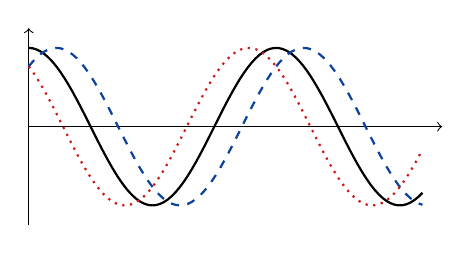
\begin{tikzpicture}[scale=0.5]
        % axis
        \draw[->] (0,0) -- (10.5, 0);
        \draw[->] (0,-2.5) -- (0, 2.5);
        % functions
        \draw[domain=0:10,black,thick,samples=100] plot (\x,{2*cos(deg(\x))});
        \draw[domain=0:10,fudanBlue,thick,samples=100,dashed] plot (\x,{2*cos(deg(\x-0.7))});
        \draw[domain=0:10,fudanRed,thick,samples=100,dotted] plot (\x,{2*cos(deg(\x+0.7))});
    \end{tikzpicture}
    \caption{实空间内波动方程的运动方向,虚线表示右移,点线表示左移}
\end{figure}
\chat{%
我们从一维单色光的平面波出发,可以第一性地给出波函数 \eqref{eq:mono_wave_sol},其中 $C$ 是光强。实空间部分是完全离域的,它是一个球谐函数,可以从 $-\infty$ 到 $+\infty$ 的震荡,其中时间的部分表示传播的方向。这种离域性用来描述光的波动性没问题,但是无法描述粒子性。}
有无定域的波也满足波动方程?

\section{光波的波包}
\subsection{波包}
动力学中常用\boldtext{波包}描述具有粒子行为的光波。定义
\begin{equation}
    \label{eq:wp_def} % wave packet definition
    \psi(x,t) = \int_{- \infty}^{+ \infty} A(k) \exp \big[ \ii \big( k x - \omega(k) t \big) \big] \, \mathrm{d} k,
\end{equation}
与单色光不同的是,其中放开了两个变量作为波数的函数——振幅 $A(k)$ 与频率 $\omega(k)$。
\chat{%
对于单色光,给定了 $k$ 就确定了 $\omega$ 和波函数,所以一个 $k$ 就相当于一个单色光。对每一个的单色光的某种振幅分布的全空间积分,即为一种光的组合,称之为波包。为何称为「包」,后面从图像上解释。

于是 $A(k)$ 是光强振幅,描述波包的形状,$\omega(k)$ 是频率,描述波包的移动速度。
}

这个波包是否满足波动方程 \eqref{eq:mono_wave}?证明之。分别对坐标和时间求偏导,有
\begin{align*}
    \frac{\partial^2\psi(x,t)}{x^2} 
    &= \int_{-\infty}^{+\infty} A(k) \frac{\partial \ee^{\ii kx}}{\partial x^2} \exp(-\ii\,\omega(k) t) \,\dd k \\ 
    &= \int_{-\infty}^{+\infty} A(k) (-k^2) \frac{\partial \ee^{\ii kx}}{\partial x^2} \exp[\ii(kx - \omega(k)t)] \,\dd k,
\end{align*}
\begin{align*}
    \frac{\partial^2\psi(x,t)}{t^2} 
    &= \int_{-\infty}^{+\infty} A(k) \ee^{\ii kx} \frac{\partial}{\partial t^2}\exp(-\ii\,\omega(k) t) \,\dd k \\ 
    &= \int_{-\infty}^{+\infty} A(k) \left[-\omega(k)\right]^2 \ee^{\ii kx} \exp[\ii(kx - \omega(k)t)] \,\dd k, 
\end{align*}
观察可知,当 $\omega(k) = ck$ 时,满足波动方程 \eqref{eq:mono_wave}。结论是,单色波的各种分布的组合同样满足波动方程。下面引入一种特殊的波包。

\suppInfo{波包与波动方程}{我们可以说,$\psi(x,t)$ 仍然是光波波动方程的解。这通过将上述 $\psi(x, t)$ 代入波动方程很容易验证。从物理的角度,事实上,如果表达式 $\omega(k) = c k$ 始终成立,那么被积函数 $\exp \big[ \ii \big( k x - \omega(k) t \big) \big]$ 就是波矢为 $k$ 的单色光。由于波动方程的特性,两个不同波矢 (或等价地说波长) 的单色光的线性叠加仍然是波动方程的解,而积分又可以看作是无数不同波长的光波的线性叠加,因此 $\psi(x,t)$ 仅仅就是复色光,它仍然满足单色光所满足的波动方程。

但是这种复色光有很有意思的特性,那就是我们可以通过合适地定义振幅 $A(k)$,使得 $\psi(x,t)$ 具有局域形状,并且该函数可以被归一化。我们应当注意到,单色光的表达式是不可归一化的,宏观上就是在全空间上宽度为常数的波形。}

\subsection{Gaussian 波包}

定义波包的振幅为 Gaussian 型函数,
\begin{equation}
    A(k) = \frac{\sqrt{a}}{(2 \pi)^{3/4}} \exp \left[ - \frac{a^2}{4} (k - k_0)^2 \right]. \label{eq:wp_gaussian_def}
\end{equation}

首先讨论,当 $t = 0$ 的时波包的情况,此时的波函数
\begin{equation}\label{eq:wp_t0}
\psi(x, 0) = \int_{-\infty}^{+\infty} \frac{\sqrt{a}}{(2 \pi)^{3/4}} \exp \left[ - \frac{a^2}{4} (k - k_0)^2 \right] \exp \left( i  k x  \right) \, \dd k. 
\end{equation}
为了求出这个积分,引入傅里叶变换(Fourier transform),
\begin{align}
    &F(x) = \int_{-\infty}^{+\infty} f(k) \ee^{\ii kx}\,\dd k, \\
    &f(k) = \frac1{2\pi}\int_{-\infty}^{+\infty} F(x) \ee^{\ii kx}\, \dd x, 
\end{align}
\chat{%
其中 $f(x)$ 右侧的 $\frac{1}{2\pi}$ 也可拆成两个 $\frac1{\sqrt{2\pi}}$、将其中一个 $\frac1{\sqrt{2\pi}}$ 乘在 $F(x)$ 右边,这是傅里叶变换的多种等价表示方式。傅里叶变换可将时域 $f$ 变换为频域 $F$,相当于一种卷积,这里仅将它用作求积分公式。
}
Gaussian 函数的傅里叶变换为
\begin{align}
    &G(k) = \frac a{\sqrt \pi} \ee^{-a^2 k^2}, \\
    &g(x) = %\frac{1}{\sqrt{2\pi}} 
    \int_{-\infty}^{+\infty} G(k) \ee^{\ii kx} \dd k =  \frac{1}{\sqrt{2\pi}} \exp\left(-\frac{x^2}{4a^2}\right), \label{eq:ift_gaussian}
\end{align}
%{Gaussian 函数的逆变换}
\begin{lstlisting}
res = InverseFourierTransform[a/Sqrt[Pi] Exp[-a^2 k^2], k, x];
Simplify[res, Assumptions -> {a > 0}]
>> E^(-(x^2/(4 a^2)))/Sqrt[2 \[Pi]]
\end{lstlisting}
因此将 $t_0$ 时的波包,拼凑成傅里叶逆变换 \eqref{eq:ift_gaussian} 的形式,有
\begin{equation}
    \psi(x, 0) = \frac{\sqrt{a}}{(2 \pi)^{3/4}}  \ee^{i  k_0 x} \int_{-\infty}^{+\infty} \exp \left[ - \frac{a^2}{4} (k - k_0)^2 + i(k-k_0)x  \right] \dd k,
\end{equation}
设 $b = \frac a2$,$l = k-k_0$,则上式为
\begin{equation}
    \psi(x, 0) = \frac{2b}{(2 \pi)^{3/4}} \ee^{i  k_0 x} \int_{-\infty}^{+\infty} 
    \ee^{-b^2l^2} \ee^{\ii l x} \dd l, 
\end{equation}
凑出 \eqref{eq:ift_gaussian} 中的形式,在积分内乘 $\frac b{\sqrt{\pi}}$,同时令 $x = - 2\pi x'$,
\begin{align}
    \psi(x,0) &= \frac{2b}{(2 \pi)^{3/4}} \ee^{\ii k_0 x} \frac{\sqrt{\pi}}b \underbrace{\int_{-\infty}^{+\infty} \frac b{\sqrt{\pi}} \ee^{-b^2l^2} \ee^{\ii l (-2\pi x')} \dd l}_{\text{inverse Fourier transform}} \\
    &= \frac{2b}{(2 \pi)^{3/4}} \ee^{\ii k_0 x} \frac{\sqrt{\pi}}b  \exp\left(-\frac{\pi^2x'^2}{4 b^2}\right) \\
    &= \left(\frac{2}{a^2\pi}\right)^{1/4} \ee^{\ii k_0 x} \exp\left(-\frac{x^2}{a^2}\right). \label{eq:wp_photon_t0}
\end{align}
\begin{lstlisting}
Integrate[
 Sqrt[a]/(2 Pi)^(3/4)
   Exp[-a^2/4 (k - k0)^2] Exp[I k x], {k, -Infinity, Infinity}, 
 Assumptions -> {a > 0}]
>> (E^(x (I k0 - x/a^2)) (2/\[Pi])^(1/4))/Sqrt[a]
\end{lstlisting}
于是我们推导出了 0 时刻的 Gaussian 波包。%,并且该波包是归一化的,
%TODO: 并不归一吧

当 $t > 0$ 时,有
\begin{equation}
    \psi (x, t) = \left( \frac{2}{\pi a^2} \right)^{1/4} \exp \left[ - \frac{(x - ct)^2}{a^2} \right] \exp [ \ii k_0 (x - ct) ]. 
\end{equation}
\homework{
    \textbf{1.2} ~  利用傅里叶变换,推导 $t>0$ 的 Gaussian 波包。
}

\begin{figure}\centering
    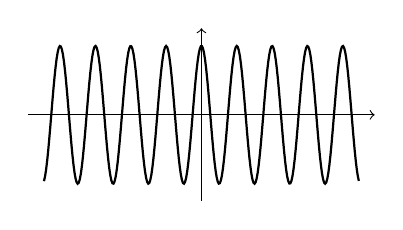
\begin{tikzpicture}[scale=0.5]
        % axis
        \draw[->] (-4.4,0) -- (4.4, 0);
        \draw[->] (0,-2.2) -- (0, 2.2);
        % functions
        \draw[domain=-4:4,black,thick,samples=300] plot (\x,{1.75*cos(deg(7*\x))});
    \end{tikzpicture}
    \begin{tikzpicture}[scale=0.5]
        % axis
        \draw[->,white] (0,-2.2) -- (0, 2.2);
        % functions
        \node[] at (0,0) {$\times$};
    \end{tikzpicture}
    \begin{tikzpicture}[scale=0.5]
        % axis
        \draw[->] (-4.4,0) -- (4.4, 0);
        \draw[->] (0,-2.2) -- (0, 2.2);
        % functions
        \draw[domain=-4:4,black,thick,samples=300] plot (\x,{1.75*exp(-0.25*\x*\x)});
    \end{tikzpicture}
    \begin{tikzpicture}[scale=0.5]
        % axis
        \draw[->,white] (0,-2.2) -- (0, 2.2);
        % functions
        \node[] at (0,0) {$=$};
    \end{tikzpicture}
    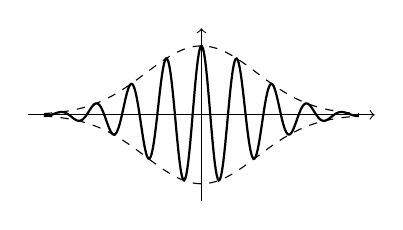
\begin{tikzpicture}[scale=0.5]
        % axis
        \draw[->] (-4.4,0) -- (4.4, 0);
        \draw[->] (0,-2.2) -- (0, 2.2);
        % functions
        \draw[domain=-4:4,black,thick,samples=300] plot (\x,{1.75*exp(-0.25*\x*\x)*cos(deg(7*\x))});
        \draw[domain=-4:4,black,samples=300,dashed] plot (\x,{1.75*exp(-0.25*\x*\x)});
        \draw[domain=-4:4,black,samples=300,dashed] plot (\x,{-1.75*exp(-0.25*\x*\x)});
    \end{tikzpicture}
    \caption{0 时刻波包的组成}
\end{figure}
\chat{%
接下来探讨这个波函数有什么样的性质。一个全空间离域的单色波矢,乘上一个高斯函数,所以形成了这样一个波包。波与波包都是以光速 $c$ 向正方向传播,并且没有任何衰减、变形,最大振幅为 $\left( \frac{2}{\pi a^2} \right)^{1/4}$。
}

\section{实物粒子的 Gaussian 波包}
\chat{%
德布罗意告诉我们,有静止质量的物体,既是波也是粒子。那么,实物粒子能不能用高斯波包来表示?单色光波的话有个很重要的关系 $\omega = kc$,频率和波矢有直接的关系,但是实物粒子不是这样的。现在我们要将光波波包向实物粒子过渡,以尝试从波动性的角度解释实物粒子。

但这里或许会遇到一个问题,实物粒子不会以 $c$ 的光速传播,因此 $\omega = ck$ 的表达式不成立。我们要如何定义角频率 $\omega$ 与波矢 $k$?
}

假设现在并不是狭义相对论的,或者说实物粒子以较低速度运动。在经典力学下,自由粒子(不受外势场 $V (x)$ 影响的粒子)的能量(即动量)为
\begin{equation}
    E = \frac{p^2}{2m} \quad \text{(粒子)},
\end{equation}
考虑波粒二象性,粒子的能量必然也有物质波所对应的能量表述,
\begin{align}
    &E = h\nu = \hbar \omega, \\
    &p = \hbar k, 
\end{align}
上两式同样也适用于无质量的光子。对于实物粒子而言,联立上面的式子消去 $E,p$ 可得
\begin{equation}
    \omega = \frac{\hbar k^2}{2m},
\end{equation}
注意到,实物粒子的波矢与角频率是平方的关系,这是与光子最大的区别。

\chat{%
同样使用波包 \eqref{eq:wp_def} 和高斯波包 \eqref{eq:wp_gaussian_def} 的原始定义,得到 $t =0$ 时刻的波函数与光波 \eqref{eq:wp_photon_t0} 是一样的,但 $t > 0$ 的波函数就完全不一样了。
}

% \subsection{精确解}
尽管积分非常复杂,但这仍然是有解析解的。当 $t > 0$ 时,
\begin{equation}
    \psi(x,t) = \left(\frac{2}{\pi a^2}\right)^4 \frac1 {\sqrt{ 1 + \dfrac{2\hbar t}{ma^2}\ii}} \exp \frac {\displaystyle -\frac{x^2}{a^2}-\frac{\ii k_0^2 t \hbar }{2 m}+\ii
    k_0 x} {1 + \dfrac{2\hbar t}{ma^2}\ii},
\end{equation}
所以概率分布为
\begin{equation}
    |\psi(x, t)|^2 = \sqrt{\frac{2}{\pi a^2}} \frac{1}{\sqrt{1 + \displaystyle \frac{4 \hbar^2 t^2}{m^2 a^4}}} \exp \left[ - \frac{2}{a^2} \frac{\left( x - \displaystyle \frac{\hbar k_0}{m} t \right)^2}{1 + \displaystyle \frac{4 \hbar^2 t^2}{m^2 a^4}} \right]. 
\end{equation}

\chat{%
我们应当得到以下的结论:
\begin{enumerate}[nosep]
  \item 指前因子可以表示波包的最大振幅。对于光波,其振幅恒定;但对于实物粒子,其振幅会依 $t$ 增长而递减,且递减的程度表现为类双曲线型;
  \item 指数项分母表示波包展宽。对于光波,其展宽恒定;但对于实物粒子,其展宽依 $t$ 增长而递增,且递增的程度表现为类双曲线型;
  \item 指数项分子表示波包的移动速度。对于光波,其移动速度为 $c$,与每个波矢 $k$ 分项的移动速度相同;而实物粒子的移动速度(波包群速度)为 $\hbar k_0 / m$,而波矢为 $k_0$ 的单色波对应的移动速度(相速度)$\omega(k_0) = \hbar k_0 / 2m$,两者相差两倍。
\end{enumerate}
}

这也就意味着,如果用 Gaussian 波包的方式描述自由粒子,即使规定 $t = 0$ 时具有较窄的波包展宽,足够长时间后也总会扩散。「足够长的时间」与物质的质量有关。假设电子的半径大约为 \SI{2.81E-15}{\metre};在一秒时间内仍然处于自由粒子状态。若使用波包解释,那么它现在的半径就在一秒钟内扩大了如下倍数:
\begin{equation}
\sqrt{1 + \frac{4 \hbar^2 t^2}{m_\mathrm{e}^2 r_\mathrm{e}^4}} 
= \sqrt{1 + \frac
{4\times(\num{1.05E-34})^2\times1}
{(\num{9.11E-31})^2(\num{2.82E-15})^4}
}
\simeq \num{2.92E25}
\end{equation}
\begin{lstlisting}
Clear[\[HBar], me, re]
\[HBar] = 1.05457182*10^-34;
me = 9.1093837*10^-31;
re = 2.8179*10^-15;
Sqrt[1 + (4 \[HBar]^2 1)/(me^2 re^4)]
>>2.91586*10^25
\end{lstlisting}
短短一秒,电子似乎会变得比太阳还要大。当然,对于宏观的物体而言,情况就不太一样了。假设一个人在宇宙大爆炸时期诞生,重 \SI{76}{\kilo\gram},想象成为 \SI{1}{\metre} 展宽的波,那么他可能在 2022 年时膨胀了 \num{7.20E-37} 倍。

\chat{%
目前为止,我们还不能说实物粒子波包的物理模型是错误的(事实上,实物粒子波包模型确实是 Schr\"odinger 方程的解)。只有当物质质量足够大、初始时刻展宽足够宽时,波包能重现经典物理的图像。但想要通过波来刻画粒子的行为,似乎会在微观世界变得不太直观。我们会说这是朴素的波粒二象性的理解,它仍然是试图将粒子通过波的行为描述,而产生看似谬误的结论。

一种可能的理解是,所谓波性与粒性不应朴素地理解,物质的行为在长时间未观测时是不可知的;而在测量时,若使用检测波形的手段就会使得波函数坍缩到接近平面光波的形式;若使用检测粒子的手段则会使波函数接近 $\delta$ 函数的粒子形貌。这称为波包的收缩;依据一些量子力学表述,这比较接近关于波函数投影的假设。

但这不仅是 Gaussian 波包的困难。事实上,对于任意的 $A(k)$ 即任意波包,当时间足够长,波包总会弥散。这可以通过求取不确定度 $\langle x^2 \rangle - \langle x \rangle^2$ 给出;这需要使用到 Ehrenfest 定理。\footnote{Cohen-Tannoudji, LIII, Exercise 4.}
}

\section{从自由粒子波函数到 Schr\"odinger 方程}

\subsection{非相对论 Schr\"odinger 方程}

Schr\"odinger 方程\textbf{不可导出} ,它一般会作为量子力学的假定出现 (尽管说从 Dirac-von Neumann 公理体系能导出 Schr\"odinger 方程)。但若我们只考虑自由电子 (即不考虑外加势场),那么 Schr\"odinger 方程某种程度上可以通过波包函数导出。

我们仍然以实物粒子的波包函数出发:
\begin{gather}
  \psi(x, t) = \int_{- \infty}^{+ \infty} A(k) \exp \big[ \ii \big( k x - \omega(k) t \big) \big] \, \mathrm{d} k \\
  E = \hbar \omega \quad p = \hbar k \\
  E = \frac{p^2}{2 m} \quad \omega = \frac{\hbar k^2}{2 m}
\end{gather}
我们希望找到一个偏微分方程,使得 $\psi(x, t)$ 是该偏微分方程的解。但需要注意到,光波方程是不可行的,譬如 $\exp \big[ \ii \big( k x - \omega(k) t \big) \big]$ 满足下述方程
\begin{equation}
\frac{\partial^2 \psi}{\partial x^2} = \frac{k^2}{\omega^2} \frac{\partial^2 \psi}{\partial t^2} \quad \mathrm{(failed)}
\end{equation}
之所以这个方程在光波上允许,但粒子上不行,是因为对于光波,$k^2/\omega^2$ 恰好是 $1/c^2$ 为常数,但对于粒子而言则为 $(2m/\hbar k)^2$,并非是常数。上述描述波函数的方程只能用于 $k$ 是唯一值的情况,不能用于包含各种不同的 $k$ 的波包因此不应当使用该方程。

但很容易地会想到,之所以会出现 $\omega^2$ 是因为 $\psi$ 对时间 $t$ 作两次偏导时,其前面的系数 $\omega$ 也就被抽提了两次 (这对于 $k$ 也是类似的)。但如果现在只对 $t$ 作一次偏导,那么就只会抽提一次 $\omega$;并且 $k^2 / \omega$ 是常数 $2m/\hbar$,因此就解决了方程中出现的与 $k$ 有关的项。

沿着这个思路,我们就尝试对 $\psi(x, t)$ 分别作 $x$ 的二阶导、$t$ 的一阶导:
\begin{align}
  \frac{\partial^2 \psi}{\partial x^2} &= - \int_{- \infty}^{+ \infty} k^2 A(k) \exp \big[ \ii \big( k x - \omega(k) t \big) \big] \, \mathrm{d} k \\
  \frac{\partial \psi}{\partial t} &= - \int_{- \infty}^{+ \infty} \frac{\ii \hbar k^2}{2 m} A(k) \exp \big[ i \big( k x - \omega(k) t \big) \big] \, \mathrm{d} k
\end{align}
因此,
\begin{equation}
\frac{\partial \psi}{\partial t} = \frac{\ii \hbar}{2 m} \frac{\partial^2 \psi}{\partial x^2}
\end{equation}
即
\begin{equation}
\ii \hbar \frac{\partial \psi}{\partial t} = - \frac{\hbar^2}{2 m} \frac{\partial^2 \psi}{\partial x^2}
\end{equation}
这就是自由粒子所满足的 Schr\"odinger 方程。


\subsection{相对论对 Schr\"odinger 方程的拓展 (Klein–Gordon)}

方才我们解决了实物波的方程;但它无法描述光波的行为。如果我们希望同时描述好光波与实物波,我们就需要使用狭义相对论的原理了。

我们先作假定:物体的运动质量 $m$ 与静止质量 $m_0$ 存在关系
$$
m = \frac{m_0}{\sqrt{1 - v^2/c^2}}
$$
整理得到
$$
\frac{m_0^2}{m^2} = 1 - \frac{v^2}{c^2}
$$
留意到 $p = mv$,那么
$$
m^2 = m_0^2 + \frac{p^2}{c^2}
$$
根据 Einstein 质能关系 $E = m c^2$,可知
$$
E^2 = m_0^2 c^4 + p^2 c^2
$$
该式原本是描述实物波的;但如果置光子质量 $m_0 = 0$,那么上式也恰好对光子成立。一般来说,光子的静止质量为零是假设,几乎没有实验现象表明光子的质量对现有理论框架产生冲击。

我们仍然认为自由粒子满足波包波函数,并且 $E = \hbar \omega, \quad p = \hbar k$;那么波包将波包波函数中的 $\omega, k$ 分别替换为 $E, p$ (留意到 $E, p$ 应当视作关于波数的变量),就得到
$$
\psi(x, t) = \int_{- \infty}^{+ \infty} A(k) \exp \big[ \frac{i}{\hbar} \big( p x - E t \big) \big] \, \mathrm{d} k
$$
容易验证,上述波函数满足
$$
\frac{1}{c^2} \frac{\partial^2 \psi}{\partial t^2} - \frac{\partial^2 \psi}{\partial x^2} + \frac{m_0^2 c^2}{\hbar^2} \psi = 0
$$

这就是 (Spin-0 的) 相对论对 Schr\"odinger 公式的拓展;由于是 Klein 与 Gordon 在 1926 年较早公开提出该公式,因此以这两人命名。事实上,该公式已经出现在 Schr\"odinger 在 1925 年的草稿中,但由于无法很好地与氢原子精细光谱进行比对 (现在认为是由自旋引起),因此 Schr\"odinger 在 1926 年仅仅发表了上述公式的非相对论的弱化版本。

我们不对上述公式在非相对论情形下与 Schr\"odinger 方程的等价性作说明;也不对真正解释了自旋现象的另一个相对论方程,即 Dirac 方程作说明。

\extraInfo{助教补充}{
\begin{itemize}[nosep]
\item 光子的能量 $E$、动量 $p$、波矢 $k$、角频率 $\omega$ 关系式:Wikipedia \href{https://en.wikipedia.org/wiki/Photon\#Relativistic_energy_and_momentum}{Photon: Relativistic energy and momentum}
\item de Brogile 对实物波的猜想:博士论文 (法语) 的英语翻译 \href{https://www.relativitycalculator.com/pdfs/On_Theory_Quanta.pdf}{\emph{On the Theory of Quanta}}
\item 通过波包理论对朴素波粒二象性的批判:\emph{唐敖庆之量子力学},徐元植,浙江大学出版社
\begin{itemize}[nosep]
    \item \S 2.1 平面波
    \item \S 2.3 德布罗意波
    \item \S 3.4 量子力学与经典力学的关系
    \item 该书中可能有公式或表述错误或不当
\end{itemize}
\item 自由实物粒子波包的讨论:\emph{量子力学(第一卷)},C. Cohen-Tannoudji 等著,刘家谟、陈星奎译,高等教育出版社
\begin{itemize}[nosep]
    \item 第一章 \S C 对一个粒子的量子描述;波包
    \item $\mathrm{G_I}$ 一维高斯型波包;波包的扩展
    \item $\mathrm{L_{III}}$ 第 4 题
\end{itemize}
\item 自由实物粒子波包的习题:\emph{量子力学概论(原书第二版)},David J. Griffiths 著,贾瑜等译,机械工业出版社,习题 2.22
\item Klein-Gordon 方程:How to Derive the Schrodinger Equation; David W. Ward, Sabine M. Volkmer; \href{https://arxiv.org/abs/physics/0610121}{arXiv:physics/0610121}
\item Schr\"odinger 方程的历史:Wikipedia \href{https://en.wikipedia.org/wiki/Klein\%E2\%80\%93Gordon_equation\#History}{Klein-Gordon equation: History}
\item 从 Dirac-von Neumann 公理导出 Schr\"odinger 方程:\href{https://en.wikipedia.org/wiki/Schr\%C3\%B6dinger_equation\#Derivation}{Schrödinger equation: derivation}
\end{itemize}

关于波函数的收缩或坍缩 (测量对波函数的影响),这在 Cohen-Tannoudji 的书中当作第五假定。

Schr\"odinger 的波动表述现在并不认为是完善的。我们的讨论是从单色光开始;但关于单色光是否能以波函数形式写出,应当认为不可以,因为函数不可归一化。费曼的路径积分表述可能可以解决该问题。
}

% \section{章节总结}
\courseTime{Sep. 19, 2022\\Week 3\\}

上周我们回顾了一下量子力学的诞生,这周课我们会讲算符、量子力学的公设。这这节课与物化AI的内容其实差不了太多,但是我们试图重新梳理,不是推导,演绎量子力学的发展历程,希望大家能加深理解。

如果大家做作业,包括对课程有任何的问题跟建议,都可以跟我们联系。

我们先来回顾上节课的内容,然后做一些基本的总结。因为每节课我也经常控制不好,有时想讲东西太多。事实上,有的关键点反而可能还会漏掉一些,所以我现在会来补一下。

上节课我们讲的,总结起来只有一页纸的内容,即量子力学的诞生。量子力学诞生,根本的地方其实就是在于对物质波粒二象性的理解,特别在微观世界中。波粒二象性最重要的关系就是 Planck--Einstein 关系式,
\begin{equation}
    E = h\nu = \hbar \omega
\end{equation}
这个公式,最早是由普朗克在拟合黑体辐射公式时,得到的一个新的物理概念。他发现,只有假设电磁波的辐射的话是一份一份进行的,才能拟合黑体辐射的频率(波长)跟辐射能之间的关系。

最重要的是说,光、电磁波,波的能量必须是一份一份的,所以每份能量跟波的频率直接成正比,并且这个相关的系数是一个常数,我们叫它 Planck 常量。后面经常会遇到 $\hbar$,$\hbar$对应的就是角频率角频率 $\omega$。
我们讲,一个粒子或者说一个东西,它是粒子。除了它的能量,那我们知道它的运动的话离不开动量。一个粒子,它的运动有方向、动量,并且动量也要满足动量守恒的规则。所以它必须有一个动量的表达式。动量的这个推导能证明,量子力学的诞生要基于相对论的诞生。没有相对论,我们没有办法直接给出光动量的方程式的。那么它到底是怎么来的呢?

在相对论的框架下面,有个质能关系。其中最重要的想法是,质量的变化满足
\begin{eqnarray}
    m = m_0 + \Delta m,
\end{eqnarray}
对于光而言的话,在相对论的框架下,
\begin{eqnarray}
    m = \frac{m_0}{\sqrt{1+\left(\frac vc\right)^2}}. 
\end{eqnarray}
所以当速度接近于光速的时候,$\Delta m \rightarrow \infty$。所以在相对论的框架下,光的初始质量一定是要为零,才能保证运动质量是常数。

对于任何物体或粒子,均有
\begin{equation}
    \left\{
        \begin{aligned}
            &\Delta E = \Delta m c^2,\\
            &p = mv,
        \end{aligned}
    \right.
\end{equation}
对于光子,
\begin{equation}
    \left\{
        \begin{aligned}
            &E = mc^2, \\
            &p = mc = \frac Ec = \frac{h\nu}c = \frac h\lambda, 
        \end{aligned}
    \right.
\end{equation}
可推知
\begin{equation}
    \left\{
        \begin{aligned}
            &E = h \nu = \hbar\omega , \\
            &p = \frac{h}{\lambda} = \hbar k, 
        \end{aligned}
    \right.
    \label{eq:photon_Ep}
\end{equation}
进而有
\begin{equation}
    \left\{
        \begin{aligned}
            &\omega = 2\pi\nu,
            &k = \frac{2\pi}{\lambda}, 
        \end{aligned}
    \right.
\end{equation}
于是 $\omega = ck$ 是线性关系。

到了实物波,我们通常处理的是在非相对论框架下的这个微观粒子——电子。目前不涉及重金属、过渡金属,特别是 F 区、镧系、锕系金属中的电子。我们通常处理氢元素中的电子,它的运动的速度是远低于光速的。
如何理解粒子的实物波?必须提到德布罗意的做法。他认为,实物也有波粒二象性,电子的干涉、衍射证明了波动的一面。波的性质是如何表述的呢?德布罗意认为,将普朗克-爱因斯坦的关系直接应用到实物波中。
以电子、质子为代表的微观粒子,静质量不为零 $m_0 \neq 0$,运动速度远低于光速导致 $\Delta m \simeq 0 |_{v \ll c}$,那么能量
\begin{eqnarray}
    E = \frac{p^2}{2m}.
\end{eqnarray}
这个公式是我们从牛顿力学就知道的。如果我们认为波动性跟粒子性是微观粒子的一体两面,那么它必定有波动的性质。那波动的性质所对应的物质波的角频率、物质波的波矢,跟粒子性是什么关系?德布罗意就把它们们两个强行耦合在一起。根据 \eqref{eq:photon_Ep},粒子的动量为
\begin{eqnarray}
    \hbar\omega = \frac{(\hbar k)^2}{2m},
\end{eqnarray}
因此得到 $\omega = \frac{\hbar k^2}{2m}$。
现在只是在演绎,怎么能够把非相对论框架下的薛定谔方程演绎出来。至于相对论框架的狄拉克方程,我们可以做其他方式的拓展。

为了更好地描述粒子实物波的粒子,上节课引入了 Gaussian 波包。我们先推导了自由粒子的波包,它的波动方程,
\begin{eqnarray}
    \psi(x,t) = A \exp[\ii (kx - \omega t)],
\end{eqnarray}
将不同波矢的自由粒子做一个全空间的积分或者组合,我们就可以得到一个波包,
\begin{eqnarray}
    \psi(x,t) = \int_{-\infty}^{\infty} A(k) \exp[\ii (k x - \omega(k) t)] \dd k,
\end{eqnarray}
最大的不同与,振幅 $A$、角频率都与波矢有关。

代入波动方程中,显然自由粒子的波包是满足的,
\begin{lstlisting}
\[Psi][x_, t_] := A Exp[I (k x - c k t)];
D[\[Psi][x, t], {x, 2}]/D[\[Psi][x, t], {t, 2}]
>> 1/c^2
\end{lstlisting}
但物质波的波包并不满足,
\begin{eqnarray}
    \frac{\partial^2 \psi}{\partial x^2} = \frac{4 m^2}{k^2 \hbar ^2} \frac{\partial^2 \psi}{\partial t^2}. 
\end{eqnarray}
\begin{lstlisting}
\[Psi][x_, t_] := A[k] Exp[I (k x - (\[HBar] k^2)/(2 m) t)];
D[\[Psi][x, t], {x, 2}]/D[\[Psi][x, t], {t, 2}]
>> (4 m^2)/(k^2 \[HBar]^2)
\end{lstlisting}
左右两个偏导并不是线性关系。

上节课推导了物质波的波包。
注意到,如果物质波对坐标求二阶偏导、对时间求一阶偏导,二者是有线性关系的,即
\begin{eqnarray}
    \frac{\partial^2 \psi}{\partial x^2} = - \ii\frac{2m}\hbar \frac{\partial \psi}{\partial t}. 
\end{eqnarray}
稍作变化,便可发现
\begin{eqnarray}
    -\frac{\hbar^2}{2m} \frac{\partial^2 \psi}{\partial x^2} = \ii\hbar \frac{\partial\psi}{\partial t},
    \label{eq:free_partial_schrodinger}
\end{eqnarray}
这是自由粒子的薛定谔方程。这个没有严格推导,只有演绎。

\chapter{算符与量子力学公设}
对于定义,我会直接陈述。对于跟宏观世界不太一样的公设、算符,我们会展开讲。
微观世界中粒子的行为可以用什么波的状态方程来描述,如何得到体系中的可观测量物理量?
我们就需要算符作用到系统的波函数上,才能得到一些信息。首先,我们必须定义到底什么是算符,我们从一些常见的算符开始讲起。
\section{常见的算符}
对一个具体的波函数,它包含了该体系所有的信息。

那么对于任意一个算符 $\hat A$,相应的物理可观测量要怎么得到?假设算符 $\hat A$ 是时间的函数,定义有
\begin{eqnarray}
    \langle A(t) \rangle = \intinf \psi^*(x,t) \ \hat{A} \ \psi(x,t) \dd x,
\end{eqnarray}
对于位置算符,有
\begin{eqnarray}
    \langle x(t) \rangle = \intinf \psi^*(x,t) \ x\  \psi(x,t) \dd x,
\end{eqnarray}
位置算符就是位置本身,所以位置算符本身不是时间的函数。因为波函数本身包含时间,所以只对实空间积分就给出了波函数随时间演化的平均位置。也就说,在粒子散射的过程中,就可以通过这个方式给出粒子的平均运动轨迹。还是要强调,后面的推导并不是证明,只是演绎,希望能够增加理解。

\subsection{动量算符的推导}
大家知道动量算符是什么样子,它为什么是这个样子状态?跟宏观动量有何关系?为何与质量无关?

现在我们先回到牛顿力学中,有
\begin{eqnarray}
    p(t) = mv(t) = m \frac{\partial x}{\partial t},
\end{eqnarray}
无论在微观世界、宏观世界,还是在非相对论框架、相对论框架,这个是普适存在的。只不过说,在微观世界里面,如果体系的速度不是本征值的时候,那么我们要对速度求期望值,也就是速度的期望值也是动量的期望值。

在牛顿力学里,速度的描述是坐标,对时间的偏导是速度。如果我们在微观世界里,因为微观世界不确定这体系是不是坐标或动量的本征函数。那怎么办呢?我们就要对它们两个同时做期望值,两个期望一定满足
\begin{eqnarray}
    \langle p(t) \rangle = m \frac{\partial \langle x(t) \rangle}{\partial t},
\end{eqnarray}
这就是动量的公式在微观世界中的描述。

代入定义,有
\begin{eqnarray}
    \langle p(t) \rangle = m \intinf \frac{\partial}{\partial t} [\psi^*(x,t)\ x \ \psi(x,t)] \dd t,
\end{eqnarray}
利用复合函数求导的定义
\begin{eqnarray}
    \frac{\partial}{\partial x} [f(x) g(x)] = \frac{\partial f(x)}{\partial x} g(x) + f(x) \frac{\partial g(x)}{\partial x},
\end{eqnarray}
得到
\begin{eqnarray}
    \langle p(t) \rangle = m \intinf x \left(
        \frac{\partial \psi^*}{\partial t}\psi + \psi^* \frac{\partial \psi}{\partial t}
    \right)
    \dd t,
    \label{eq:pt_ave_2}
\end{eqnarray}
按照自由粒子的薛定谔方程 \eqref{eq:free_partial_schrodinger}, 上式 \eqref{eq:pt_ave_2} 有
\begin{align}
    & \frac{\partial \psi^*}{\partial t} = - \frac{\ii \hbar}{2m} \frac{\partial^2 \psi}{\partial x^2}, \\
    & \frac{\partial \psi}{\partial t} = \frac{\ii \hbar}{2m} \frac{\partial^2 \psi}{\partial x^2}, 
\end{align}
代回 \eqref{eq:pt_ave_2} 有
\begin{eqnarray}
    \langle p(t) \rangle = -\frac{\ii\hbar}{2} \intinf x \left( \psi \frac{\partial^2\psi^*}{\partial x^2} - \psi^* \frac{\partial^2\psi}{\partial x^2}\right) \dd x
    \label{eq:pt_ave_3}
\end{eqnarray}
约掉了质量 $m$。再次利用复合函数求导,设 $f(x) = \psi^*(x,t)$,$g(x) = \frac{\partial^2 \psi}{\partial x}$,则
\begin{align}
\frac{\partial}{\partial x}(f g) = \frac{\partial}{\partial x}\left(\psi^* \frac{\partial^2 \psi}{\partial x^2}\right) = \psi^* \frac{\partial^2\psi}{\partial x^2} + \frac{\partial \psi^*}{\partial x} \frac{\partial \psi}{\partial x}, 
\end{align}
于是有
\begin{align}
    &\psi^* \frac{\partial^2 \psi}{\partial x^2} = \frac{\partial}{\partial x} \left(\psi^*\frac{\partial \psi}{\partial x}\right) -\frac{\partial \psi^*}{\partial x} \frac{\partial \psi}{\partial x}, \\
    &\psi \frac{\partial^2 \psi^*}{\partial x^2} = \frac{\partial}{\partial x} \left(\psi\frac{\partial \psi^*}{\partial x}\right) - \frac{\partial \psi}{\partial x} \frac{\partial \psi^*}{\partial x},
\end{align}
代回 \eqref{eq:pt_ave_3} 有
\begin{eqnarray}
    \langle p(t) \rangle = \frac{\ii\hbar}2 \intinf x \frac{\partial}{\partial x} \left(\psi^* \frac{\partial \psi}{\partial x} - \psi \frac{\partial \psi^*}{\partial x}\right) \dd x,
    \label{eq:pt_ave_4}
\end{eqnarray}
设 $f(x) = \psi^* \frac{\partial \psi}{\partial x} - \psi \frac{\partial \psi^*}{\partial x}$,数学上显然有
\begin{eqnarray}
    \frac{\partial}{\partial x}[x f(x)] = f(x) + x \frac{\partial f(x)}{\partial x},
\end{eqnarray}
所以 \eqref{eq:pt_ave_4} 为
\begin{eqnarray}
    \langle p(t) \rangle = \frac{\ii\hbar}2 \intinf \frac{\partial}{\partial x}(x f(x)) \dd x - \frac{\ii\hbar}2 \intinf f(x) \dd x,
    \label{eq:pt_ave_5}
\end{eqnarray}
其中第一项为 $x f(x) | ^{+\infty}_{-\infty}$。

\suppInfo{波函数的有限性}{
对于实际的原子分子体系,波函数必须在无穷远处趋于 0。比如坐标的平均值
\begin{eqnarray}
    \langle x(t) \rangle = \intinf \psi^*(x,t) \ x\  \psi(x,t) \dd x = \intinf x \rho(x,t) \dd x
\end{eqnarray}
是偶极,必然为有限值 $\psi^* x \psi |_{x \rightarrow \pm \infty} = 0$。同理,$\langle x^2 \rangle$为电四极,也必须为有限值。总之,波函数必须在无穷远处为 0。那么 $ \psi^*\psi|_{x=\pm\infty} \propto 1/x^s, s>2 $ ,应当比$ 1/x^n $更快衰减。}

于是 \eqref{eq:pt_ave_5} 为
\begin{eqnarray}
    \langle p(t) \rangle = - \frac{\ii\hbar}2 \intinf \left(\psi^* \frac{\partial \psi}{\partial x} - \psi \frac{\partial \psi^*}{\partial x}\right) \dd x,
\end{eqnarray}
再利用分部积分,有
\begin{align}
    \langle p(t) \rangle &= \frac{\ii\hbar}2 \intinf \left(\frac{\partial}{\partial x}(\psi\psi^*) - \frac{\partial \psi}{\partial x}\psi^* - \psi^* \frac{\partial \psi}{\partial x}\right) \dd x \\
    &= \psi\psi^* |_{-\infty}^{\infty} + \frac{\ii\hbar} 2 \intinf \left(-2\psi^* \frac{\partial \psi} {\partial x} \right)\dd x \\
    &= \intinf \psi^* \left(-\ii\hbar \frac{\partial}{\partial x}\right) \dd x,
\end{align}
那么 $\hat p = - \ii\hbar \frac{\partial}{\partial x}$。
通过动量的定义、薛定谔方程,便可演绎出动量算符。

动能算符
\begin{eqnarray}
    \hat T = \frac{\hat p^2}{2m} = -\frac{\hbar^2}{2m} \frac{\partial ^2}{\partial x^2}
\end{eqnarray}
即薛定谔方程左边。

\section{含势函数的 Schr\"odinger 方程表达式}%与波函数空间-时间分离}
% credit: ZY Zhu

经过上述的演绎,可以知道非相对论自由粒子的薛定谔方程为
\begin{equation}
\ii \hbar \frac{\partial \psi}{\partial t} = \frac{\hat p^2}{2 m} \psi,
\end{equation}
其中的 $\hat p^2 / 2m$ 与经典力学中的动能项 $E = p^2 / 2m$ 非常相似。而经典力学中,哈密顿量可以写为动能项加势函数项。

类似地在上述方程中引入势函数 $V(x, t)$:
\begin{equation}
\ii \hbar \frac{\partial \psi}{\partial t} = \hat H \psi = \left( \frac{\hat p^2}{2 m} + V(x, t) \right) \psi
\end{equation}
上式就是含有势函数的、一般的 Schr\"odinger 方程,同时也定义了哈密顿算符 $\hat H$。它不只可以解释自由粒子,也可以解释受限粒子 (譬如一维势箱),但无法拓展到相对论的情形。化学中通常所使用的量子力学的最根源的表达式即上述 Schr\"odinger 方程。

特别地,讨论一种常见且特殊的情况,即势函数 $V(x, t) = V(x)$ 不随时间变化。势函数不随时间变化的例子,如自由的或外加静电场的分子电子运动过程,而势函数随时间变化的例子,如分子受光激发的过程。

当 $V(x, t) = V(x)$ 时,我们说该方程存在分离变量的 (空间-时间分离的) 波函数解。假定
\begin{equation}
\psi(x, t) = \phi(x) f(t),
\end{equation}
代入到 Schr\"odinger 方程,得到
\begin{equation}
\ii \hbar \phi(x) \frac{\partial f(t)}{\partial t} = - \frac{\hbar^2}{2 m} \frac{\partial^2 \phi(x)}{\partial x^2} f(t) + V \phi(x) f(t)
\end{equation}
两边分别除以 $\psi = \phi f$,得到
\begin{equation}
\frac{\ii \hbar}{f(t)} \frac{\partial f(t)}{\partial t} = - \frac{\hbar^2}{2 m} \phi(x) \frac{\partial^2 \phi(x)}{\partial x^2} + V 
%= \frac{\hat H \phi}{\phi}
\end{equation}
该式左右分别是只关于 $t$、$x$ 的函数。因此,若要让等式成立,则等式两边必为常数。该常数我们定作 $E$,因为哈密顿算符相当于表示体系的能量 (作为守恒量),
\begin{align}
    &\hat H \phi(x) = E \phi(x), \\
    &\pdv{t} f(t) = -\frac{\ii E}\hbar f(t),
\end{align}

那么,时间部分解得
\begin{equation}
f (t) = \exp \left( - \frac{i}{\hbar} E t \right),
\end{equation}
空间部分解得
\begin{equation}
\hat H \phi(x) \equiv \qty(- \frac{\hbar^2}{2 m} \pdv[2]{x} + V (x)) \phi(x) = E \phi(x)
\end{equation}
称为\boldtext{定态} Schr\"odinger 方程。

\extraInfo{推导}{
这两节课我一直在重复物化 A I 前几节课的内容,但是这里用一些比较数学演绎的方式,推导出方程的建立过程。

我希望大家能够体会其中的创造性,这个创造性是超越于一般的演绎和推理。现在经常讲机器学习、人工智能,人工智能为什么被认为说是有前途的一门学问呢?就是说它希望超越一般的规律,去寻找复杂大数据背后的一种数据到结果的映射关系。这个映射关系如果找到足够好,是不是可以从中得到一些物理?

对于物理、化学、生物,是研究物质的科学。为什么说化学叫中心学科呢?因为它下面是可以承接物理,往上可以承接更复杂的生物。「中心学科」只个是一个中性词,并不代表它最重要。整个过程三位一体,所有理论都是要以实验为基础开展科研工作。从实验中测得一种理论,同时要反过来解释甚至指导实验。

我们现在推导的薛定谔方程本身就是从实验中间抽取出来的,这是非常典型的范例。同时,后面也通过很多的推导去告诉大家,这里蕴含理论到底是有多强大,进而可以解释多少实验。这就是量子化学方向常常要做的事情,即解释化学中的现象。
}

不失一般性的将$ \hat p, \hat T, \hat V $从一维拓展到三维,则
\begin{align}
\hat p &= -\ii\hbar \left(\pdv{x}\vb{i} + \pdv{y}\vb{j} + \pdv{z}\vb{k}\right) = -\ii\hbar \bm\nabla, \\
\hat T &= -\frac{\hbar^2}{2m}\nabla^2, \\
\hat V &= V(x,y,z)
\end{align}
三维薛定谔方程 (3D SE)
\begin{equation}
\hat H \psi %= - \frac{\hbar^2}{2 m} \left( \frac{\partial^2 \phi}{\partial x^2} + \frac{\partial^2 \phi}{\partial y^2} + \frac{\partial^2 \phi}{\partial z^2} \right) + V (x, y, z) \phi 
\equiv - \frac{\hbar^2}{2 m} \nabla^2 \psi + V (x, y, z) \psi = E \psi,
\end{equation}
其中波函数可分离变量,写成\boldtext{定态} stationary 波函数与时间分量的乘积,
\begin{equation}
\psi(x,t) = \phi(x) \exp \qty( -\dfrac{i}{\hbar} Et).
\end{equation}
%这也是在物理化学 A I 课程中讨论得最多的方程,也是这门课程中最为重要的方程。
上述是单粒子的情形,如果是多粒子,可推广至
\begin{equation}
\qty( -\sum_i \dfrac{\hbar^2}{2m_i}\nabla_i^2 + V(x_1, \cdots, x_n)) \psi(x_1,\cdots,x_n) = E \psi(x_1,\cdots,x_n)
\end{equation}

% How. 这样我们已经可以把体系的确定了方程。
% 方程全部就给出来了对吧,因为它的这个试函数有可能是时间的关方程,所以它的哈密的方程有可能时间的方程。
% 特别的,如果我们的示函数与时间无关,那么我们就可以推出哈密顿的双层的话,也与时间无关,就等于动量上浮加上 VX 对吧。那么我们就可以翻成带带着。
% 好在这方向我们要再做一次,你们物化 AE 里面已经学过了,学过的这个变量分离变量了对吧,左边跟时间无关,右边跟时间有跟坐标无关对吧算幅我说的算幅,那么我就不失一般性的,可以把不函数写成什么,时间跟空间的层级吗?
% 对吧?那带入上时左边跟时间无关,我就可以把时间提前当成常量。
% 右边跟空间无关。
% 好了,现在我们做这个事情,下一步就要把左边的右边分开,左边右边分开,就是要让左边的 FT 消耗掉,右边的 yx 消耗掉。那这个两边同时重乘向重是除向整体的波函数。对吧。
% 这是 tree 那么就有,就可以导出这个的话就是。 Up np.
% 由此我们已经把坐标跟时间分开成两边,两边是无关的两个量,它们两个要相等,就意味着这两个要同时等于一个常数,否则的话他们是没法做这样的一个连力的。那么背后的意思就是我要把它分成两个方程了。
% 对吧,这两个方程好了,对于方程。
% 对方乘 2 我们知道说这样的一个形式,我们就可以 push 一般性的设置的 FT 为 A 乘上 ESP 的 at 对吧。那么把这个带进去就变成是其实这个也不用 A 到时候再说规划。就是 AFT 等于负I。
% A 等于负的 IE 除上H8,所以 FT 就等于。
% 那么方程1。
% 就是它的叫做定态确定和方式,因为它跟时间补完了对吧。
% 当然由此我们其实已经给出体系的再说一遍,我们现在其实这两节课我一直在重复,就是像固化 A1 里面很可能才第一节或者第二节的课对吧。但是这边我们用一些比较数学的一个演绎的方式,需要把那个早期这样的一个确定的方程的推导,这个过程的话展开来了解一下。
% 我希望大家能够体会细品中间的就是一种创造性,这个创造性的话是超越于一般的这种演绎跟推理。其实包括现在经常讲继续学习人工智能。人工智能为什么被认为说其实是挺有前途的一门学问呢?就是说他其实希望就是超越一般的规律,去寻找什么复杂的大数据背后的一个纷繁的数据背后的一种什么映射关系数据到结果的映射关系。那这个映射关系中如果找到足够好,是不是可以从中认得到一些物理?这个是蛮有意思的一个情况。因为我们对于我们物理化学是物理数学都是物理化学生物,我们称之为什么学科物质科学,物质科学可能是研究物质为主的一门科学。那我们为什么说化学叫中心学科呢?因为它是承接。
% 其实这个是一个中性词,并不代表它最重要,而正是因为说它是承接了什么物理的以及下面是可以承接物理,晚上是承接,晚上是可以承接更为复杂的生物对吧?那么整个过程那三三位一体其实背后对应就是所有东西都是要以所有都要以什么实验为基础开展的科研工作对吧?那么实验从实验中测一种理论的理论,同时要反过来的话解释甚至指导实验。那我们现在的确定和方程本身就是从从实验中间抽取出来的理论的一个非常典型的范例。然后同时我们后面也通过很多的证明,很多的那个推导去告诉大家这个这样的一个范例的话,推导得到的理论到底是有多强大,到底是可以真的解释多少实验?那么这就是后面我们做的量子化学里面常常要做的事情,就解释化学中的一些现象。那么有了定态学定要方程,我们这么还要再做一步对吧。因为真实的世界是什么?三维的世界首先它不是一维的。那么我们当然要不是一般性的干嘛把这些算图从一维的干嘛变成三维的,那这个是 strike forward 对吧。
% 那动量上浮。
% Full ih bar. 我们就要对它。 Exo. rising sandwich go to panda 那么我们就引入一个新的上浮的模式。
% 定态的,我们现在后面这节课,这次这门课我们根本都碰不到磐石的,当然下节课除外,所以我们这边就做这样的一个简单的定义。由此我们已经有了这个设定二方程的三维的普遍的普适的形式,动能算服加势能算服。
% 对。这边就是从这个应该就是单例子体系对吧,他的这个定态确定和方程当地词体系在真实世界中的定态确定和方程。那么由此我们其实已经可以把确定和方程的话。
% Particular culture in.
% 之所以称为定态训练方程,就是因为它的波函数并不包含时间。
% Stationery stay.
% 有了这些我们就可以开始讲这个前面我们就到这里为止,我们其实是把算幅的一些演绎给大家了。往下我们就要引入什么?为了完整性,一门课还是要完整性,可能大家已经学过了,那我们就是还要把算法的定义重新的抽题出来描述一下,以及它的一些基本的规则。
% 算幅的定义。算幅定义从本质上来讲的话,就是干嘛把一个函数干嘛变成了另外一个函数对吧,就它是把一个函数变另外还有一个操作。那么所以原则上说 A 可以是任何一个东西,可以是标量,可以是函数,可以是泛函。泛函的意思就是说它可以是根号偏微分之类的到动量动能上浮就是一个偏微分对吧?那么我们这边就有了到底它的代数规则。
% 上浮的和与差,就是说设。
% 那么这个算幅如果 C 等于 A 加 B 那么它做 C 作用在任何一个函数上,就是等于 A 作用的函数上加上 B 中文函数上,这个是不言而喻的对吧,也不需要说任何的。也就是说 C 无论是任何的一个函数算幅,它都满足这个。 Mm.
% 算符的乘法。设 C 等于 A 乘上 B 那么 C 就用在函数上,就等于把 A 跟 B 依次作用的函数先是 B 作用的函数上,然后 A 作用在 B 作用过之后的函数。
% 那么一般情况。
% 交换率是不成立的对吧?一般情况是这样,我们什么时候是这样的?如果这个函数比如说是一个坐标算幅跟势能算幅,它肯定是可以的对吧是吧?那么我们经常会讲的就是说如果我们的算幅一个是偏微分的算幅, B 的话就是一个坐标算幅。那么。
% 就在任何一个函数上,它是什么?它应该是这个 FX 加上 X 对吧?那它其实是等于什么呢? In jiangxi.
% 那另外一边的话,如果是 xa 先作用到这个函数上,那么它就是。
% 对吧?所以它们并不相等这个。当然我相信你们学过物化 A 一定知道这个乘法,它们交换率不成立。其实本身的话就对于说微观世界里面很多新颖的这种这样的现象对吧,比如说他的不完备性,他的这个他的测不准,甚至于什么后面的还有零点能这些东西都跟这相关,这后面慢慢会展开来讲。
% 等价上浮。若 A 作用到 F3 等于 B 作用的 F3 对于任意。
% 对任意函数都成立。
% 我们就说 A 等就是等于 B 好吧,那就像这边我们说的上面这个式子的话,这个是我们对于任一个函数做下来的对吧,FX我们没有定 FX 是什么东西好,所以这边就有就知道说这个。
% 就带 xm 等于什么这两个上头对吧,是等价的。
% 当我们在定义这个算幅空间的时候,为了完备性起见,我们肯定要定义它的什么单位算法称为单位算法,据说 1 就是它的单位算法。
% Unit operator tong shi ling weikong sanfu.
% Now operate. 同时我们这边做个约定,对于常数的算法。
% 我们都不加这个帽子。那么我们从前面也可以看到说这个。
% 就等于零,就是一个空胀符。好,那么上浮的最后的定义的话,行吧,那我们下节课再讲好。
% 作业的话,我会在下节课布置。
% 哪一个?就是那个减 1 等于就是那个半 X 那个减 1 等于0。
% 没就展示他们两个算不加价是完整,这只是为了完备性。其实后面可能到时候在后面会用到一些,但是本质上的话就是表示说这两个上浮是等价的,他们相应点基本是什么都没有,就是零售这是上浮空间。为了完备,你现在我们定义放射空间,我们只会定义说我们的那这块是要空间,我们定义的空间一定要给他完整全是数学项的一个,就是事实上我们用的不多。Ok。
% 然后之前那个就是那就是猜猜是分离的这是,时空分离什么地方不明白。
% 我说我也有问题。
% 行,大概就是就是从就是这里的话,把它变量分离之后。

到目前为止,我们已经演绎得到一些常见的算符。为了这门课的完整性,还要把算符的定义和基本规则重新抽提出来描述一下。


\section{算符的定义}
算符从本质上来讲,是把一个函数变成另外一个函数的操作。原则上说算符 $\hat A$ 可以是任何东西,可以是标量、函数、泛函等。如果算符是泛函,是说它可以是根号、偏微分之类的操作,比如动量算符就是偏微分。
\subsection{代数规则}

\begin{theorem}[算符的和与差]
    定义 $\CC = \AA + \BB$,那么
\begin{eqnarray}
    \CC u = \AA u + \BB u. 
\end{eqnarray}
\end{theorem}

\begin{theorem}[算符的乘法]
    设 $\CC = \AA \BB$,那么
\begin{eqnarray}
    \CC u = \AA\BB u = \AA (\BB u)
\end{eqnarray}
\end{theorem}

相信同学们学过物化一定知道这个乘法的交换律不成立,微观世界有很多新颖的现象,比如不完备性、测不准,甚至于后面会讲到的零点能等。

比如 $\AA = \frac{\partial}{\partial x}, \BB=x$, 有
\begin{align}
    \hat A \hat B f(x) &= \pdv{x} [x f(x)] = \qty(1 + \hat x \pdv{x}) f(x) \\
    \hat B \hat A f(x) &= x \pdv{x} f(x)
\end{align}

\begin{theorem}[等价算符]
    若 $\AA f=\BB f$ 对任意函数均成立,那么 $\AA =\BB$。
\end{theorem}
如
\begin{eqnarray}
    \frac{\partial}{\partial x} = 1 + \frac{\partial}{\partial x}.
\end{eqnarray}

\begin{theorem}[基本算符]
    单位算符 unit operator $\hat 1 = 1$,空算符 null operator $\hat 0 = 0$,常数算符通常不加 $\hat\cdot$。
\end{theorem}

% 
% 上午回顾了量子力学的诞生。
% 通过波粒二象性,隐入了实物波的波动方程,演绎出来薛定谔方程。
% 由此确立了微观粒子的状态也可以用波动方程描述。
% 对于波函数,状态与可观测量的关系,需要将算符作用上去,这是物化一的课程。
% 早上第二个内容就是演绎了动量算符为什么是偏微分的形式,并由一维拓展到高维,给出了定态薛定谔方程。
% 后面量化的大部分时间都会围绕定态薛定谔方程的求解,从定态薛定谔放成功可以得到物理化学光谱的信息。

% 第二部分,看一下算符的数学规则。
% 上午看了和差的定义是显而易见的,算符作用在函数上等于另一个函数,所以算符是定域的。$A$ 作用上去和 $B$ 作用上去是独立的。但是乘法不一样,$\hat A\hat B$ 依次作用上去。

% 一个典型的例子是导数算符和位置算符,导数算符可类比于之前推导的动量算符。

在其它表象下,算符本身可以构成完备集,算符本身可以描述微观状态,因此算符有各种加减乘除、单位元的定义,自然而然还有逆算符的定义。

\begin{theorem}[逆算符]
    设 $\hat A\hat B f(x) = f(x)$,我们就说 $\hat A = \hat B^{-1}$ 或 $\hat B = \hat A^{-1}$。
\end{theorem}

因此引申出很重要的概念\boldtext{对易}。

\begin{theorem}[对易]
    \begin{equation}
        [\hat A, \hat B] \equiv \hat A \hat B -\hat B \hat A
    \end{equation}
    若 $\hat A \hat B = \hat B \hat A$ 则$[\hat A,\hat B] = 0$,则称算符 $\hat A, \hat B$ 互易,否则不互易。
\end{theorem}

简单的例子,$\hat A = \frac{\partial}{\partial x}, \hat B = 3$,则二者互易。若 $\hat A = \frac{\partial}{\partial x}, \hat B = \hat x$, 则 $[\frac{\partial}{\partial x},\hat x] = 1$。

\homework{
    \textbf{1.} 请简化下列定义的算符 $\hat B$
    \begin{equation}
        \hat A = \frac{\partial}{\partial x} x, 
        \hat B = \hat A^2
    \end{equation}
    计算对易子 
    \begin{equation}
        \left[x^3, \frac{\dd}{\dd x}\right], \left[\frac{\dd}{\dd x}, 5x^2 + 3x + 4\right]. 
    \end{equation}
}
交换不成立,于是有了互易子的规律。以上是对于最普适算符给出的定义。

\subsection{线性算符}

对于量子力学中的算符,引入约定\boldtext{线性算符},指分别作用在两个函数上,
\begin{equation}
    \hat A [f(x) + g(x)] = \hat A f(x) + \hat A g(x)
\end{equation}
这个与加和有什么不同?加和是对所有算符成立,但是上式仅对线性算符成立。线性算符是说,一个算符作用在两个函数上,相当于分别作用在两个函数上。

引入线性算符的重要性:\boldtext{量子力学中所有具有物理意义的算符都是线性算符}。有一个重要的性质
\begin{equation}
    \hat A [C f(x)] = C\hat A f(x)
\end{equation}
\begin{equation}
    \hat A[ \underbrace{f(x) + \cdots + f(x)}_{C} ] = C\hat A f(x)
\end{equation}
哪些不是?$\sqrt{\cdot}, (\cdot)^2, \sin, \cos$ 等,比如
\begin{equation}
    \sqrt{f(x) + g(x)} \neq \sqrt{f(x)} + \sqrt{g(x)}. 
\end{equation}

哥本哈根诠释,表示波函数的平方表示概率。波函数本身没有物理意义,算符作用上去才有物理意义。

如果 $\hat A$ 是本征态,那么必然有
\begin{eqnarray}
    \hat A f(x) = A f(x), \\
    \hat A C f(x) = AC f(x)
\end{eqnarray}
任何的缩放也都是本征态,如果是非线性算符则无法满足。对于波函数而言,最重要的概念是叠加,干涉、衍射,是线性加和的,如果波函数不是线性的,那么波函数就不满足后面要学的量子力学公设。

有了这样的线性算符,就可以给出算符的\boldtext{左右分配律},
\begin{eqnarray}
    (\hat B + \hat C) \hat A = \hat B \hat A + \hat C \hat A,
\end{eqnarray}
左右分配律对任何算符一定成立,但是右分配律仅对线性算符成立。
\begin{eqnarray}
    \hat A (\hat B + \hat C)  \neq \hat A \hat B + \hat A \hat C,
\end{eqnarray}
算符里量化中用得不多,如果以后做实验,实验中越来越向微观调控发展。当你去操控分子,你的操作就对应于算符,需要先设计算符,算符必须是微观可观测的。可以做一些先验的设计,否则实验是不可能成立的。
\homework{\textbf{2.} 证明算符的左右分配律}

\subsection{Hermitian 算符与量子力学公设}

\begin{theorem}[Hermite 算符]
    对于任意给定的(合理)波函数 $u$,若算符满足
\begin{eqnarray}
    \int u^* \hat A u \dd \tau = \int(\hat A u)^* u \dd t,
\end{eqnarray}
则 $\hat A$ 为Hermite 算符。
\end{theorem}

如动量 $\hat p = -\ii \hbar \frac{\partial}{\partial x}$、动能 $\hat T = \frac{\hat p^2}{2m}$、哈密顿算符 $\hat H$。
\homework{\textbf{3.} 证明上述三个算符为 Hermite 算符}

为什么我们要隐入 Hermite 算符的定义?
清晰的客观物理事实,所有的物理可观测量都对应 Hermite 算符,期望值一定是实数。对应着
\begin{align}
    &\left\langle A\right\rangle = \int \psi^* \hat A \psi \dd \tau, \\ 
    &\left\langle A\right\rangle^* = \int \psi (\hat A \psi)^* \dd \tau = \int (\hat A \psi)^* \psi \dd \tau,
\end{align}
若 $\hat A$ 非 Hermite 则
\begin{eqnarray}
    \left\langle A\right\rangle \neq \ev{A}^*
\end{eqnarray}
$\ev{A}$ 不是实数,进而 $\hat A$ 不对应物理可观测量。

我们讨论的大部分算符不只是 Hermite 的,也都是线性的。
\homework{\textbf{4.} 对于线性的 Hermite 算符 $\hat A$,我们有
\begin{eqnarray}
    \int u ^* \hat A \nu \,\dd \tau = \int (\hat A u)^* \nu \,\dd \tau,
\end{eqnarray}
同时,对于线性的 Hermite 算符,$\hat A, \hat B$ 具有以下性质,
\begin{enumerate}
    \item $\hat A + \hat B$ 仍是 Hermite 算符
    \item $[\hat A, \hat B] = 0$,$\hat A\hat B$ 与 $\hat B \hat A$ 仍是 Hermite 算符
\end{enumerate}

\textbf{5.}
    若 $\hat A, \hat B, \hat C$ 为线性算符
    \begin{enumerate}
        \item 若 $\hat A, \hat B$ 同时为 Hermite 算符,则 $\hat A \hat B + \hat B \hat A$ 与 $\ii [\hat A \hat B - \hat B \hat A]$ 都是 Hermite 算符
        \item $[\hat A, \hat B \hat C] = \hat B [\hat A, \hat C] + [\hat A, \hat B]\hat C$
        \item $[\hat A \hat B, \hat C] = \AA[\BB,\CC] + [\AA,\CC]\BB$
        \item $[\AA,[\BB,\CC]] + [\BB,[\CC,\AA]] + [\CC, [\AA, \BB]] = 0$
    \end{enumerate}
}

Hermite 算符之后,还有个重要的约定。

\subsection{Dirac 记号}

它是用来描述期望值。如果算符作用在波函数上,
\begin{eqnarray}
    \int \phi_m^* \hat A \phi _n \dd\tau = \langle \phi_m | \hat A | \phi _m \rangle \equiv \langle m | \hat A | m \rangle \equiv A_{mn}
\end{eqnarray}
如果 $m = n$ 则表示期望值,如果不等于则表示跃迁矩阵元,
\begin{eqnarray}
    A_{mn} \equiv \langle m | \hat A | n \rangle
\end{eqnarray}
% $\langle \phi_m | \hat A | \phi _m \rangle$ Dirac 记号,$A_{mn}$ 矩阵元表述,$\langle m | n \rangle = \int \phi_m^* \phi_n \dd\tau$ 重叠积分。所以
左矢表示 $\langle m| = \phi_m^*$ 波函数的共轭,右矢表示 $\ket{m} = \phi_m$ 波函数。还有更多自由的写法,
$\hat A n$ 自身可以看成一个函数,
\begin{eqnarray}
    \langle m | \hat A | n \rangle = \langle m | \hat A n \rangle,
\end{eqnarray}

所以 Dirac 记号右矢 $|n\rangle$ 代表波函数 $\phi_n$(即 $\hat A \phi_n$),左矢 $\langle m |$ 代表波函数 $\phi_m$(即 $\hat A \phi_m$)的共轭。

% \begin{eqnarray}
%     \int u^* \hat A \nu \dd\tau = \int(\hat Au)^* \nu \dd\tau, \\
%     \langle u | \hat A | u \rangle = \langle \hat A u | u \rangle = [][][][]
% \end{eqnarray}

通过 Dirac 记号,可以写出 Hermite 算符的定义:
\begin{equation}
  \langle m | \hat A n \rangle = \langle \hat A m | n \rangle = \langle n | \hat A m \rangle^* = \langle m | \hat A^* n \rangle
\end{equation}
对于 Hermite 算符而言,$\hat A = \hat A^*$。

但需要留意的是,当 $\hat A = \partial_x$ 即导数算符时,$\hat A^* = - \partial_x$;因此算符的共轭并非简单地将虚数单位 $\ii$ 替换为 $-\ii$。

我们把量子力学里算符简单过一遍。假设物化一里都学过,为了课程完整性所以需要讲一遍。这里跟以前学的有何不同?如果没有问题,下节课会讨论量子力学公设。如果有时间,我们会讨论物理意义和一些具体例子。

实验归纳总结了许多公理体系,即量子力学公设。目前还没有遇到违反公设的情况。多种公设的表述方式,在数学证明中都是等价的。

\begin{theorem}[公设1]
    一个量子力学体系,均可用一个含时的波函数 $\psi(\vec r, t)$ 来描述,该函数应是单值、连续和有限的品优波函数。
\end{theorem}

\begin{theorem}[公设2]
对于一个量子体系,每一个可观测力学量都对应一个线性 Hermite 算符与量子力学公设
\end{theorem}

\begin{theorem}[公设3]
当对量子体系的某一力学量进行测量时,每次可测一数值 $\lambda$ 则 $\lambda$ 与该力学量对应的算符以及波函数 $\psi$ 之间存在如下关系
\begin{eqnarray}
    \hat F \psi =\lambda \psi
\end{eqnarray}
即 $\lambda$ 是 $\hat F$ 的本征值,而 $\psi$ 是 $\hat F$ 的本征函数。
\end{theorem}

以前有同学问:为什么实验中的基态在测完之后还是在基态?化学中的实验,为什么能提前知道物质处在基态,为什么没有不确定性?比如为什么物质的生成焓都是确定的?我觉得这个问题非常好。

\begin{theorem}[公设4]
对于任意一个线性 Hermite 算符,其本征方程
\begin{eqnarray}
    \hat F \psi_i = \lambda_i \psi_i
\end{eqnarray}
的本征函数 $\{\psi_i\}$ 均构成一个完备集,对于任意一个波函数,
\begin{eqnarray}
    \Psi = \sum_i c_i \psi_i
\end{eqnarray}
都可以可以展开
\end{theorem}

这是一个非常强的定理,有它物理意义。一个原子的哈密顿算符,我们在物化1中解出了各种轨道。按第四点来说,这个完备基是在全空间展开的,也就是任何体系都可以用氢原子的完备基展开。比如两个相距一定距离的氢原子,物理上来说用两个波函数叠加是最好的,但从第四点来说,用一个原子的波函数来展开也是完全可行的。实际上,因为波函数是无穷多的,必须用无穷多才能完全描述,因此可以这么描述,但不是最高效的。

\subsection{Hermite 算符}
给出 Hermite 算符的特殊性质。不推导,留一些给同学们证明。

\begin{theorem}[a]
    线性 Hermite 算符的本征函数 $\{\psi_i\}$ 一定是正交归一的,Dirac 记号表述为
\begin{align}
    &\langle i | i \rangle = 1, \\
    &\langle i | j \rangle = 0, \quad i \neq j
\end{align}
推知
\begin{eqnarray}
    \delta_{ij} = 
    \left\{
        \begin{matrix}
            1, i=j,\\
            0, i\neq j
        \end{matrix}
    \right.,
\end{eqnarray}
\end{theorem}

\begin{theorem}[b]
    若$\psi$ 是算符 $\hat F$ 的本征值 $f$ 的本征函数,
\begin{eqnarray}
    \hat F \psi = f \psi,
\end{eqnarray}
则对 $\psi$ 体系,$\hat F$ 的一次测量肯定($100\%$)测得 $f$ 值。
\end{theorem}

\begin{theorem}[c]
若 $\Psi$ 不是 $F$ 的本征函数,按照第四点完备基的定义,总是可以表述成
\begin{eqnarray}
    \Psi = \sum_i c_i \psi_i, \quad\langle \Psi | \Psi \rangle = 1
\end{eqnarray}
如果是归一的,利用正交归一的性质
\begin{align}
    \langle \Psi | \Psi \rangle &= \Big\langle \sum_i c_i \psi_i \Big| \sum_j c_j \psi_j \Big\rangle \\
    &= \sum_i \sum_j c_i^* c_j \langle \psi_i | \psi_j \rangle \\
    &= \sum_i \sum_j c_i^* c_j \delta_{ij} \\
    &= \sum_i |c_i|^2 = 1.
\end{align}
\end{theorem}
算符的期望值
\begin{eqnarray}
    \langle F\rangle = \langle \Psi | \hat F | \Psi \rangle = \sum_i |c_i|^2 f_i. 
\end{eqnarray}
如果波函数并不是算符 $\hat F$ 的本征函数,每进行一次测量,平均值即为上式,每次测得的值为 $f_i$,概率为 $c_i$。

薛定谔猫是处在生态和死态叠加中,如果猫的状态是生和死的叠加,它并不是一定生或死的。那么数学上来说,我对某状态做某测量得到某值的概率是多少。

我们知道,动量算符和位置算符互易,不能同时测量,换句话说,它们不能同时拥有相同的本征函数。如果对动量的本征函数做位置的测量,也就是把位置的算符作用到动量的本征函数上去。
假设所有东西都是离散的。设 $\{\phi_i\}$ 为 $\hat p$ 的本征函数,一定不是位置算符的本征函数。将坐标作用上去,平均值为 $\int \phi_i^* \hat x \phi_i \dd \tau$。位置算符 $\hat x$ 的本征函数 $\{f_m\}$,将动量的本征函数展开为 $\phi_i = \sum_m c_i f_i$,所以在某个动量的本征函数 $\phi_i$ 上找到位于 $x_m$ 电子的概率就是 $|c_m|^2$,
测量后就有 $|c_m|^2$ 概率坍缩到 $f_m$ 上去。这个时候再测量位置,那么这个体系将永远处在 $f_m$ 上了。
如果再去测量动量,重新展开成 $f_m = \sum_i c_i \phi_i$,动量是全空间覆盖的,那么就有 $|c_i|$ 的概率处在 $\phi_i$ 态上。

我们在讨论化学问题的时候,总是在说基态能量、生成热,因为我们是对能量算符进行测量,所以基态的能量是不会变的,除非是基态和激发态的耦合或者是散射过程。

\begin{theorem}[d]
    若两个线性 Hermite 算符有一个共同的本征函数完备集,则两个算符可以对易,
\begin{eqnarray}
    \hat F \psi_i = f_i \psi_i. \hat G \psi_i = g_i \psi_i,
\end{eqnarray}
则二者互易 $[\hat F, \hat G] = 0$ 或二者可以同时测量
\end{theorem}

\homework{\textbf{6.} 证明 (a) 与 (d)}

为什么单值、连续、有限很重要?去年讲太慢了,很多没讲到。
我们用哥本哈根的统计诠释,讲品优波函数的物理内涵。

其实波函数本身没有物理意义,波函数的平方是概率,有物理意义。
\begin{eqnarray}
    |\psi (x,t)|^2 = \psi ^*(x,t) \psi(x,t)
\end{eqnarray}
为概率密度 probability density,在 $t$ 时刻 $x$ 位置到 $x + \dd x$ 为之内发现粒子的概率,
\begin{eqnarray}
    |\psi(x,t)|^2\dd x = \text{Pr}(\dd x; x; t)
\end{eqnarray}
在区间 $[a,b]$ 内发现例子的概率,
\begin{eqnarray}
    \int_a^b |psi(x,t)|^2 \dd x = \text{Pr} (a \leq x \leq b, t)
\end{eqnarray}
全空间的概率和
\begin{eqnarray}
    \int_{-\infty}^{\infty} |\psi(x,t)|^2 \dd x = 1
\end{eqnarray}
$\psi$ 是归一化的 normalized。

由这些定义出发,品优波函数有哪些约束?

a) $|\psi|^2$ 是概率密度,可知 $|\psi(x,t)|^2 \dd x$ 有限。那么这个约定,是否意味着波函数在任何一点都要有限呢?实际上并不是很重要,其背后的数学表述是波函数必须平方可积的 square-integrable,才能保证波函数可以归一。这里有例外吗?第一节课我们就碰到过,自由粒子是全空间发散,下节课会讨论到。

在量子力学中,并不排除会使用某些不能归一化的波函数。\footnote{曾谨言 \S 2.1.6; Levine \S 2.4, \S 3.8}一个重要的例外就是自由粒子。波函数有限的定义可能不是很严谨。

\suppInfo{波函数一定为有限值才能平方可积吗?}
{
    假设在三位空间中 $x_0 $ 处,波函数存在孤立奇点 $ |\Psi(x_0)|^2 \rightarrow \infty $。看似违反了「有限」的公设,实际上,
	只需要 $\int_{\tau_0} |\psi(x)|^2 \dd[3] x$ 为有限值,在物理上就可以接受,
	$ \tau_0 $为包围$ x_0 $附近的任意小体积。
	
	取$ x_0 = 0 $,在球坐标下展开,
	\begin{align}
	\int_{\tau_0} |\psi(x)|^2 \dd[3] x &= \int_0^\pi \int_0^{2\pi} \int_0^{r_0} |\Psi(r,\theta,\phi)|^2 r^2\dd r \sin\theta\dd\theta \dd\phi \\
	&\propto \int_0^{r_0} |\Psi(r)|^2 r^2 \dd r \\
	&\propto \frac{r^3}{3} |\Psi(r)|^2 \Big|_0^{r_0}
	\end{align}
	当$ r_0 \rightarrow 0 $时,$r_0^3 |\psi(r_0)|^2 \rightarrow 0$,设 $\psi(r_0)| \rightarrow \frac1{r_0^s}$,则 $r_0^3 \frac{1}{r_0^{2s}} \rightarrow 0$,解得 $s < \frac32$。

    对于其它维度,可解得 二维$ s < 1 $、 一维$ s < \frac{1}{2} $。
}

b) 当 $x\rightarrow\pm\infty, \psi(x,t)\rightarrow0$,积分是全空间的,并且最终是有限的,所以在无穷远处一定为0。如果在无穷远处不为 0,肯定积分发散的。所以这一条也是概率密度推导出来的。

c) 为了满足哥本哈根学派的统计解释,要求归一化,全空间模的积分为1
\begin{eqnarray}
    \int_{-\infty}^{\infty} |\psi(x,t)|^2 \dd x = 1,
\end{eqnarray}
但归一化并不像想象中自发成立的。

问题,如果波函数在 $t = 0$ 是归一化的 $\int_{-\infty}^{\infty} |\psi(x,0)|^2 \dd x = 1$,那么它时间演化中的每一刻 $t>0$ 是否都是归一化的?请证明
\begin{eqnarray}
    \frac{\partial}{\partial t} \int_{-\infty}^\infty |\psi(x,t)|^2 \dd x =0, \rightarrow \int_{-\infty}^\infty \frac{\partial}{\partial t} |\psi|^2 \dd x =0,
\end{eqnarray}

证明,
% \begin{eqnarray}
%     \frac{\partial}{\partial t}|\psi|^2 = \psi \frac{\partial}{\partial t} \psi^* + \psi^* \frac{\partial}{\partial t}\psi
% \end{eqnarray}
% 代入薛定谔方程,有
% \begin{align}
%     &\ii\hbar \frac{\partial}{\partial t} \Psi = -\frac{\hbar^2}{2m} \frac{\partial^2}{\partial x^2} \psi + V(x) \psi, \\
%     &\frac{\partial}{\partial t} \psi = \frac{\ii\hbar}{2m} \frac{\partial^2\psi}{\partial x^2} - \frac{\ii}{\hbar} V(x) \psi, \\
%     123
% \end{align}
% 将后两式子代回 [][][],则有 【】【很长的式子,】【】
Schr\"odinger方程具有保持波函数归一化的特性。\footnote{顾樵 \S 2.1.2}证明如下

    	随时间演化满足含时薛定谔方程
    	\begin{equation}
    	\ii\hbar \pdv{t} \Psi = -\frac{\hbar^2}{2m} \pdv[2]{x}\Psi + V\Psi
    	\end{equation}
由
    \begin{align}
    \pdv{t} \Psi &= \dfrac{\ii\hbar}{2m} \pdv[2]{x} \Psi - \dfrac{\ii}{\hbar} V(x) \Psi \\
    \pdv{t} \Psi^* &= -\dfrac{\ii\hbar}{2m} \pdv[2]{x} \Psi^* + \dfrac{\ii}{\hbar} V(x) \Psi^*
    \end{align}
得
    	\begin{align}
    	&\phantom{=}\pdv{t} |\Psi(x,t)|^2  \\
        &= \pdv{\Psi^*}{t}\Psi + \Psi^*\pdv{\Psi}{t}  \\
    	&= \Psi \qty(-\dfrac{\ii\hbar}{2m} \pdv[2]{x} \Psi + \dfrac{\ii}{\hbar} V(x) \Psi) + \Psi^* \qty(\dfrac{\ii\hbar}{2m} \pdv[2]{x} \Psi - \dfrac{\ii}{\hbar} V(x) \Psi) \\
    	&= \dfrac{\ii\hbar}{2m} \qty[\Psi^*\pdv[2]{\Psi}{x} - \Psi\pdv[2]{\Psi^*}{x}] \\
    	&= \dfrac{\ii\hbar}{2m} \pdv{x} \qty[\Psi^*\pdv{\Psi}{x} - \Psi\pdv{\Psi^*}{x}]
    	\end{align}
那么
    \begin{align}
    \pdv{t} \intinf |\Psi(x,t)|^2 \dd x &= \intinf \dfrac{\ii\hbar}{2m} \pdv{x} \qty[\Psi^*\pdv{\Psi}{x} - \Psi\pdv{\Psi^*}{x}] \dd x \\
    & = \dfrac{\ii\hbar}{2m} \qty[\Psi^*\pdv{\Psi}{x} - \Psi\pdv{\Psi^*}{x}] \Big|_{-\infty}^\infty \\
   &= 0 
    \end{align}
 所以$ \intinf |\Psi(x,t)|^2 \dd x  $不依赖于时间。证毕。

甚至可以讲到高斯定理。

下节课真正开始求解真正体系了,我们会做一些拓展,展开数学推导中的黑箱。




% \section{复习}
\courseTime{Sep. 26, 2022\\Week 4}
%2022-09-26 07:59:45  Wenbin Fan @FDU 
早上好。人少了一点,我们都是选了这课的。

第一次课回顾了量子力学的诞生,我们想从量子力学初期实验现象演绎出薛定谔方程。其中最重要的现象是波粒二象性。光波的波动方程是两个二阶偏导呈线性,薛定谔方程是二阶偏导、一阶偏导有线性关系。

如果势函数 $V$ 与时间无关,那么则可以分离时间和坐标,对于仅包含坐标的方程为定态薛定谔方程。如果是自由粒子

2021 年,\emph{Science} 发布了《125 个问题:发现与发现》,其中 ``What is quantum uncertainty and why is it important?'' 是其中一个问题。\footnote{\url{https://www.science.org/content/resource/125-questions-exploration-and-discovery}}目前的量子计算、量子测量是热门领域。
\extraInfo{什么是量子不确定性,为什么它很重要?}{
海森堡不确定性原理是量子力学的一个关键原则,它指出我们不能同时测量一个物体的速度和位置。天文学家和科学记者Ethan Siegel写道:``你越是精确地测量一个物体的位置,你对其动量的了解就越是内在不准确。这不仅仅是我们仪器的失败,这种不确定性是宇宙的根本。''不确定性在量子计算中起着重要作用,它依靠电子叠加来存储信息。但是量子叠加是很棘手的事情。当你试图测量它们时,或者甚至通过与环境的共同作用,如遇到随机的电磁辐射脉冲,它们会坍缩(用量子术语)。
}

我们讲过了高斯波包。通过高斯波包一阶、二阶偏导之间的关联,我们演绎出了薛定谔方程,并且演绎出了光波可以回到麦克斯韦的波动方程。对于质量不为零的粒子,利用德布罗意物质波、波矢与角频率是二次关系,推出了薛定谔方程。

上次课讲了量子力学的公设,算符的定义。

1. 微观体系都需要波函数描述

2. 可观测量对应于线性 Hermite 算符。坐标、势函数的算符就是本身。 能量与动量的关系,$E = mc, p = h/\lambda$,加上薛定谔方程可推导出$\hat p = -\ii \hbar \frac{\partial}{\partial x}$

3. $\AA f = \lambda f$ 本征方程

4. 线性 Hermite 算符的本征函数 $\{\left|\phi_i\right\rangle\}$ 构成完备集,相同坐标空间和时间空间的系统内的任何一个粒子状态都可以表示成线性算符本征值的先行真开 $\ket{\psi} = \sum_i c_i \ket{\phi_i}$,由此就有关于测量的一些讨论。

下周放掉一节课,我们尽量讲两节课的内容。很多结论会直接给大家。

\chapter{粒子的平动}

\section{一维自由粒子}

势函数为 0,定态薛定谔方程
\begin{eqnarray}
    -\frac{\hbar}{2m} \frac{\partial}{\partial x^2}\psi(x) = E \psi(x),
\end{eqnarray}
设波函数 $\psi(x) = \ee^{s x}$,得到
\begin{eqnarray}
    s = \pm \frac{\ii}{\hbar} \sqrt{2m |E|}
\end{eqnarray}
利用德布罗意关系 $E = p^2 / 2m, p = \hbar k$,推出
\begin{eqnarray}
    E = \frac{\hbar^2k^2}{2m},
\end{eqnarray}
则
\begin{eqnarray}
    s = \pm \frac{\ii}{\hbar}|p| = \pm \ii |k| = \ii k,
\end{eqnarray}
正负号表示方向,所以正向波矢自身为正,前面符号也为正,故脱掉了绝对值符号,那么波函数为
\begin{eqnarray}
    \psi(x) = \ee^{\ii kx},
\end{eqnarray}
与负方向的波函数构成通解为
\begin{eqnarray}
    \psi(x) = C_1 \ee^{\ii kx} + C_2 \ee^{-\ii kx}
\end{eqnarray}
表示向右和向左传播的波。利用欧拉公式 $\ee^{\ii\theta} = \cos\theta + \ii\sin\theta$,展开为
\begin{eqnarray}
    \psi(x) = (C_1 + C_2) \cos kx + \ii (C_1 - C_2) \sin kx.  
\end{eqnarray}
\begin{lstlisting}
Subscript[C, 1] Exp[I k x] + 
  Subscript[C, 2] Exp[-I k x] // ExpToTrig
>> Cos[k x] Subscript[C, 1] + I Sin[k x] Subscript[C, 1] + 
 Cos[k x] Subscript[C, 2] - I Sin[k x] Subscript[C, 2]
\end{lstlisting}

\subsection{流密度}
流密度是说密度跟概率随时间流动的速度,对应着速度的概念。

回忆第一节课,我们讲到量子力学公设时提到,
状态波函数必须是正交归一的,意味着演化过程中的归一性质是不变的。使得
\begin{eqnarray}
    \int_{-\infty}^\infty |\psi(x,t)|^2 \dd x = 1
\end{eqnarray}
$\psi$ 归一化是不会随时间演化而破坏的,需要满足
\begin{eqnarray}
    \frac{\partial}{\partial t} \int_{\infty}^\infty |\psi|^2 \dd x = 0
\end{eqnarray}
概率必然大于零,可以将偏导放进去,
\begin{eqnarray}
    \int_{\infty}^\infty \frac{\partial}{\partial t}  |\psi|^2 \dd x = 0
\end{eqnarray}
有
\begin{eqnarray}
    \frac{\partial}{\partial t} |\psi|^2 = \frac{\partial}{\partial t} \psi^* \psi = \frac{\partial \psi^*}{\partial t}\psi + \psi^* \frac{\partial \psi}{\partial t}
\end{eqnarray}
代入薛定谔方程
\begin{eqnarray}
    \ii\hbar \frac{\partial}{\partial t} \psi = \left[
        -\frac{\hbar^2}{2m} \frac{\partial^2}{\partial x^2} + V(x,t)
    \right]
    \psi(x,t)
\end{eqnarray}
得到
\begin{eqnarray}
    \frac{\partial}{\partial t} |\psi|^2 = \frac{\ii\hbar}{2m} \frac{\partial}{\partial x}
    \left[
        \psi^* \frac{\partial \psi}{\partial x} - \psi \frac{\partial \psi^*}{\partial x}
    \right]
\end{eqnarray}
这是个很重要的式子,在哥本哈根诠释中,$|\psi|^2 = \rho(x,t)$ 是密度,所以粒子密度随时间的演化可以表示为
\begin{eqnarray}
    \pdv{t} \rho(x,t) = \pdv{x} \left[
        \frac{\ii\hbar}{2m} \left(
            \psi^* \pdv{\psi}x - \psi\pdv{\psi^*}x
        \right)
    \right]
\end{eqnarray}
对时间的偏导等于对坐标的偏导。流体力学中连续性方程
\begin{eqnarray}
    \frac{\partial \rho}{\partial t} + \frac{\partial J}{\partial x} = 0, 
\end{eqnarray}
其中流密度为
\begin{eqnarray}
    J = -\frac{\ii\hbar}{2m} \left( \psi^* \frac{\partial \psi}{\partial x} - \psi \frac{\partial \psi^*}{\partial x}\right)
\end{eqnarray}
应用高斯定理,可得连续性方程的积分形式
\begin{eqnarray}
    \underbrace{\frac{\partial}{\partial t} \underbrace{\int_V \rho \dd^3x}_{\substack{\text{粒子在体积} \\ \text{$V$ 中的概率}}} }_{\substack{\text{粒子流入或流出}\\ \text{体积 $V$ 的速度}}} 
     + 
    \underbrace{\oint_S \underbrace{J}_{\substack{\text{粒子流入或流出}\\ \text{体积 $V$ 的通量}}} \dd a}_{\text{围绕体积 V 的面积分}} = 0,
\end{eqnarray}
如果能够满足这个偏微分方程的平衡连续方程,该方程给出 $J$ 的定义就对应于粒子流入或流出某区域的速度。当体积固定、面积变大,速度的通量就变小了。这里的 $J$ 便是流密度。

对 $J$ 简单演绎,
\begin{align}
    J &= -\frac{\ii\hbar}{2m} \left( \psi^* \frac{\partial \psi}{\partial x} - \psi \frac{\partial \psi^*}{\partial x}\right) \\
    &= \frac{1}{2m} \left[
        \psi^* \left(-\ii\hbar\frac{\partial}{\partial x}\right) \psi +
        \psi \left(-\ii\hbar\frac{\partial}{\partial x} \psi\right)^*
    \right] \\
    &= \frac1{2m} \left[\psi^* \hat p \psi + (\hat p\psi)^* \psi\right]
\end{align}
因此,描述粒子运动的流密度可以由动量算符构造出来。

代入自由粒子的状态方程,
\begin{eqnarray}
    \psi(x,t) = a \exp (\ii k x) \exp \left( - \frac{\ii\hbar^2k^2}{2m}t\right), \quad k\hbar = p = mv,
\end{eqnarray}
%2022-09-26 08:33:07  Wenbin Fan @FDU
有
\begin{eqnarray}
    J = -\frac{\ii\hbar}{2m} [|a|^2 \ii k + |a|^2 \ii k] = \frac{\hbar k} m |a|^2 = |a|^2 v
\end{eqnarray}
流密度与速度成正比,可将 $J$ 看成粒子的运动速度。

可观测量对应的都是 Hermite 线性算符。某算符 $\AA$ 的期望值为,作用到状态波函数上并全空间积分,当且仅当状态函数为算符的本征函数时,算符作用上去得到本征值和本征函数。那么 $J$ 也应该当作算符,但是为什么没有?因为恰好自由粒子时动量函数的本征函数,所以全空间积分是一样的。

但是我们遇到了归一化问题。

\subsection{归一化问题}
\begin{eqnarray}
    \int_{-\infty}^\infty \psi^*\psi \dd x = |a|^2 \int_{-\infty}^\infty \dd x
\end{eqnarray}
显然是不可归一化的。按照量子力学公设第一条,品优波函数描述微观粒子性质,但这里不能归一。所以结论是,不存在处于定态(给定 $k$)的自由粒子。
这里有些简单粗暴了,我们算出来是这个微观状态,但因为不能归一所以就断言不存在这样的状态。

对光而言,它没有初始状态,可以描述成这个状态。对粒子而言,波是内禀属性,不意味着静止的时候可以离散到全空间。我们推过光波的波包,随时间演化永远不会发散的。粒子的波包随时间弥散,这是不对的。

但是,不处于定态的自由粒子并非不可描述。自由粒子的定态波函数是动能算符 $\hat T$ 的本征函数,
\begin{eqnarray}
    \left\{\psi(x,t) = a \exp (\ii k x) \exp \left( - \frac{\ii\hbar^2k^2}{2m}t\right)
    \right\},
\end{eqnarray}
因为 $\hat T$ 是 Hermite 算符,所以构成完备集。任何一个粒子,不处于定态,就可以展开成全空间求和
\begin{eqnarray}
    \psi_0 (x,t) = \sum_k c_k\psi_k(x,t) = \int_{-\infty}^\infty c_k\psi_k (x,t) \dd k = \int_{-\infty}^\infty A(k) \psi_k(x,t) \dd k, \label{eq:wave_expand_fullSet}
\end{eqnarray}
表示成波包的样子。

这里有很多个人看法,不见得完全正确。我能保证最终结论是对的,保证数学推导肯定不错,但中间阐述是见仁见智的问题。本来量子力学背后就有很多种不同的解释。

假设一个粒子,我们准备好了它的初态,再也不给它任何的束缚,那么该粒子的演化一定遵循薛定谔方程。
%2022-09-26 08:44:08  Wenbin Fan @FDU

% 休息
% 第二节课 % 2022-09-26 08:53:53  Wenbin Fan @FDU

准备初态,
在实空间的表示形式
\begin{eqnarray}
    \psi(x,0) = \frac{1}{\sqrt{2\pi}} \intinf A(k) \ee^{\ii kx} \dd x, 
\end{eqnarray}
利用反 Fourier 变换关系,得到微观粒子处在第 $k$ 个态的概率,也就是在 $k$ 空间(动量空间)的概率分布,
\begin{eqnarray}
    A(k) = \frac{1}{\sqrt{2\pi}} \intinf \psi(x,0) \ee^{\ii kx} \dd x,
\end{eqnarray}
结合量子力学公设第四条,任何波函数都可以由另外一组波函数线性展开。

%2022-09-26 08:58:34  Wenbin Fan @FDU
构造一个自由粒子的初态,
\begin{eqnarray}
    \psi(x,0) = 
    \begin{cases}
        \frac1{\sqrt{2a}},\quad &x\in[-a,a],\\
        0, \quad &\text{其它}
    \end{cases}
\end{eqnarray}
这是一个阶梯函数,积分得到
\begin{eqnarray}
    A(k) = \frac1{\sqrt{2a}} \frac{\sin ak}{k}
\end{eqnarray}
在 $k$ 空间却是一个全空间的正弦函数,这在通讯领域中的数模转换时常用。
有了 $A(k)$ 之后可以用来构造波函数,参考式子 \eqref{eq:wave_expand_fullSet}
\begin{eqnarray}
    \psi(x,t) = \frac1{\sqrt{2\pi}} \intinf A(k,t) \ee^{\ii k x} \dd k. 
\end{eqnarray}

讨论 (1) 如果 $a$ 很小,束缚在很窄的一个范围内,那么
\begin{eqnarray}
    A(k) = \frac{1}{\pi a} \frac{\sin ak}{k} \approx \frac{\sqrt{a}}{\sqrt\pi}
\end{eqnarray}
与 $k$ 无关,表示动量展宽很大、不确定,位置确定

(2) 如果 $a$ 很大,
\begin{eqnarray}
    A(k) = \sqrt{\frac{a}{\pi}} \frac{\sin ak}{ak}
\end{eqnarray}
当 $k\rightarrow 0$ 时,$A(k)$ 取极大值,即 $|A(k)|^2$ 取极大值。此时位置不确定,动量确定。

\homework{
    \textbf{3.1}  对于给出下述初态 $\psi(x,t=0)$,即初始时刻自由粒子($V(x) = 0$)波函数,求出 $\psi(x,t)$ 含时演化波函数,其中 $a>0, b\in\mathbb{R}, x\in\mathbb{R}$,

    (a) $A \ee^{-a|x|}$, (b) $A\ee^{-ax^2}$, (c) $A \ee^{-ax^2} \ee^{-\ii b x}$. 
}

% 2022-09-26 09:09:14  Wenbin Fan @FDU
\section{一维势箱中的粒子}
\begin{figure}[tp]\centering
    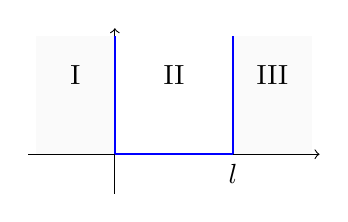
\begin{tikzpicture}[scale=0.5]
        % region
        \fill[lightgray] (-2,0) rectangle (0,3);
        \fill[lightgray] (3,0) rectangle (5,3);
        % axis
        \draw[->] (-2.2,0) -- (5.2, 0);
        \draw[->] (0,-1) -- (0, 3.2);
        % potential
        \draw[thick,blue] (0,0) -- (3,0);
        \draw[thick,blue] (0,0) -- (0,3);
        \draw[thick,blue] (3,0) -- (3,3); 
        % text
        \node[] at (-1,2) {I};
        \node[] at (1.5,2) {II};
        \node[] at (4,2) {III};
        
        \node[below] at (3,0) {$l$};
        % functions
        % \draw[domain=-4:4,black,thick,samples=100] plot (\x,{\x*\x});
    \end{tikzpicture}
    \caption{无限深势阱}
    \label{fig:inf_well}
\end{figure}
微观体系都是由品优波函数描述。
不管如何,先写出薛定谔方程。
\begin{eqnarray}
    \hat H \psi = (\hat T + V) \psi = E \psi,
\end{eqnarray}
势能函数
\begin{eqnarray}
    V(x) =
    \begin{cases}
        0, \quad &x\in [0,l]\\
        \infty, \quad &\text{其它}
    \end{cases}
\end{eqnarray}
薛定谔方程写为
\begin{align}
    (V-E) \psi &= \frac{\hbar^2}{2m} \pdv[2]{x} \psi \\
    \psi &= \frac{\hbar^2}{2m(V-E)} \pdv[2]{x} \psi,
\end{align}
对于 block I 和 III,$\psi(x) = 0$,对于 block II 有 
\begin{eqnarray}
    \psi(x) = C_1 \ee^{\ii k x} + C_2 \ee^{-\ii k x} = A \cos kx + B \sin kx,
\end{eqnarray}
这个解是普适的,导致体系量子化的是\boldtext{边界条件}。
%2022-09-26 09:15:15  Wenbin Fan @FDU
由边界条件来约束系统呈现出的状态,否则通解没有使用价值。

根据品优波函数的要求,波函数必须连续,
\begin{eqnarray}
    \psi(0) = \psi(l) = 0,
\end{eqnarray}
在 $x=0$ 处有
\begin{eqnarray}
    \psi(0) = A \cos 0 + B \sin 0 = 0,
\end{eqnarray}
立刻可得 $A = 0$,波函数为 $\psi(x) = B \sin kx$。在 $x=l$ 处,
\begin{eqnarray}
    \psi(l) = B \sin kl = 0,
\end{eqnarray}
得到量子化条件
\begin{eqnarray}
    k l = n \pi \rightarrow k = \frac{n\pi}{l}
\end{eqnarray}
其中 $n$ 为整数,所以该体系是量子化的。当 $n=0$ 时,舍去。由于 $n$ 为负时与 $n$ 为正时一样,没有新的物理,故令 $n \in \mathbb{N}^+$。得到解
\begin{eqnarray}
    \psi_n(x) = 
    \begin{cases}
        B \sin \frac{n\pi x}l, \quad &x \in [0,l], n\in\mathbb{N}^+, \\
        0,\quad &\text{其它}
    \end{cases}
\end{eqnarray}
% 【讨论为何只需要原函数连续,不需要高阶连续】【录音 1h 26min】
% 【n=0 为啥要舍去?补充】

\subsection{一维势箱的性质}

(1) 归一化 $\left\langle \psi_n \middle | \psi_n \right\rangle = 1$, 即
\begin{align}
    &= B^2 \int_0^l \sin^2 \frac{n\pi x}{l} \dd x \\
    &=  B^2 \int_0^l \left[\cos 0 - \cos \frac{2 n \pi x}l \right] \dd x \\
    &= \frac l2 B^2 + 0 = 1
\end{align}
其中利用了三角函数的变换
\begin{eqnarray}
    2\sin\alpha \sin\beta = \cos(\alpha-\beta) - \cos(\alpha+\beta),
\end{eqnarray}
因此,归一化条件为 $B = \pm \sqrt{\frac2l}$,波函数重写为
\begin{equation}
    \phi_n(x) = \begin{cases}\displaystyle
        \sqrt{\frac 2l} \sin\frac{n\pi x}l, \quad &x\in[0,l], n\in \mathbb{N}^+,\\
        0, \quad&\text{其它},
    \end{cases}
\end{equation}
注意到,归一化条件只与 $l$ 有关,与量子数 $n$ 无关。
\begin{lstlisting}
(* 画出一维势阱的波函数,n=0,...,5 *)
l = 1; (* 宽度 *)
Plot[Table[Sqrt[2/l] Sin[(n \[Pi] x)/l], {n, 0, 5}] // Evaluate, {x, 0, l}, Filling -> Axis]
\end{lstlisting}

(2) 不同量子数的波函数之间正交

当 $m \neq n$ 时,
\begin{align}
    \left\langle \psi_n \middle | \psi_n \right\rangle 
    &= \intinf \psi_n^* (x) \psi_m(x) \dd x \\
    &= \frac2l \int_0^l \sin \frac{n\pi x}{l} \sin \frac{n\pi m }{l} \dd x, \\
    &= \frac 1l \int_0^l \left[
        \cos \frac{(n-m)\pi x}l - \cos\frac{(n+m)\pi x}l
    \right] \dd x \\
    &= 0
\end{align}
因此波函数之间均满足正交归一,
\begin{eqnarray}
    \left\langle \psi_n \middle | \psi_n \right\rangle = \delta_{mn} = \begin{cases}
        1, \quad &m=n,\\
        0, \quad &m\neq n,
    \end{cases}
\end{eqnarray}

(3) 动量算符的平均值为 0
\begin{align}
    \ev{\hat p} 
    &= \left\langle \psi_n \middle| \hat p \middle| \psi_n \right\rangle \\
    &= - \ii \hbar \int_0^l \cos\frac{n \pi x}l \frac{\partial}{\partial x} \cos \frac{n\pi x}l \dd x \\
    &= \ii\hbar \frac{n\pi}l \int_0^l \cos \frac{n\pi x}l \sin\frac{n\pi x}l \dd x \\
    &= \frac{\ii\hbar}2 \frac{n\pi}l \int_0^l \left(\sin\frac{2n\pi x}{l} - \sin 0\right)\dd x \\
    &= \frac{\ii\hbar}2 \frac{n\pi}l \left(- \cos \frac{2n\pi x}l\right) \bigg|_0^l = 0,  
\end{align}
\begin{lstlisting}
Clear["Global`*"]
res = Integrate[
    Cos[(n \[Pi] x)/l] (-I \[HBar]) D[Cos[(n Pi x)/l], x], {x, 0, l}]
Simplify[res, Assumptions -> {n \[Element] Integers}]
>> 1/2 I \[HBar] Sin[n \[Pi]]^2
>> 0
\end{lstlisting}
其中利用了积化和差
\begin{equation}
    \sin\alpha \, \cos\beta = \frac12 \sin(\alpha+\beta) + \frac12 \sin(\alpha-\beta),
\end{equation}
所以流密度算符的平均值也为 0。

(4) 动量绝对值的平均值不为 0

首先求出动量平方的平均值,
\begin{align}
    \ev{\hat p^2} &= \langle \psi_n | \hat p^2 | \psi_m \rangle \\
    &= \frac{n^2\pi^2\hbar^2}{l^2} = \frac{n^2h^2}{l^2}
\end{align}
所以动量绝对值的平均值为
\begin{align}
    \rightarrow |p| = \sqrt{\ev{\hat p^2}} = \frac{n\hbar}{2l},
\end{align}
\begin{lstlisting}
res = 
Integrate[
    Sqrt[2/l] Cos[(n \[Pi] x)/l] (-I \[HBar])^2 D[
    Sqrt[2/l] Cos[(n Pi x)/l], {x, 2}], {x, 0, l}]
Simplify[res, 
    Assumptions -> {n \[Element] Integers}] /. {\[HBar] -> h/(2 Pi)}
>> (n \[Pi] \[HBar]^2 (2 n \[Pi] + Sin[2 n \[Pi]]))/(2 l^2)
>> (h^2 n^2)/(4 l^2)
\end{lstlisting}
即物质波长 $|p| = \frac{h}{\lambda}$, 得到 $\lambda = \frac h{|p|} = \frac{2l}n$。 

\extraInfo{不确定关系}{
    求出以下算符的平均值,
    \begin{align}
        &\ev{x} = \frac l2, \quad \ev{x^2} = \frac{1}{6} l^2 \left(\frac{3}{\pi^2 n^2}+2\right), \\
        &\ev{p} = 0, \quad \ev{p^2} = \left(\frac{n \pi\hbar}l\right)^2,
    \end{align}
    因此坐标和动量的涨落为
    \begin{align}
        &\sigma_p^2 = \ev{p^2} - \ev{p}^2 = \left(\frac{n \pi\hbar}l\right)^2, \\
        &\sigma_x^2 = \ev{x^2} - \ev{x}^2 = \frac{l^2}2 \left( \frac16 + \frac1{n^2\pi^2} \right),
    \end{align}
    所以不确定关系
    \begin{align}
        \Delta x \Delta p = \frac{\hbar}2 \sqrt{2+\frac{n^2\pi^2}3 } \ge \frac{\hbar}2
    \end{align}
    得到了验证。
}

(5) 能量的平均值

直接利用前面求解出的动量平方的平均值,有
\begin{align}
    E_n = \langle \hat T \rangle = \frac1{2m} \ev{\hat p^2} = 
    \frac{n^2h^2}{8ml^2}
\end{align}

(a) 由于 $n=0$ 不被允许,$E_1 = \frac{h^2}{8ml^2}$ 为\boldtext{零点能},

(b) 能级差
\begin{align}
    \Delta E_n = E_{n+1} - E_n = (2n+1) \frac{h^2}{8ml^2}
\end{align}
逐渐增大,表示能量不连续的情况越来越严重,这偏离了从量子到经典变化的过程。


(6) 粒子密度分布
\begin{eqnarray}
    \rho(x) = |\psi(x)|^2 = \frac 2l \sin^2 \frac{n\pi x}l, x\in[0,l]
\end{eqnarray}
波函数在区间 $(0,l)$ 中存在 $n-1$ 个节点,节点即 $\psi(x) = 0$ 的位置。观察易知,波函数的最大曲率与量子数 $n$ 有关,因此量子数越大,最大曲率也会越大。
\begin{lstlisting}
(* 粒子密度 *)
l = 1;
Plot[Table[2/l Sin[(n \[Pi] x)/l]^2, {n, 1, 5}] // Evaluate, {x, 0, 
  l}, Filling -> Axis]
\end{lstlisting}
当量子数趋于无穷,物质波波长越来越短,行为越像粒子,但是对于当前体系的波函数并不是这样。考察
\begin{eqnarray}
    \frac{\Delta E}{E} = \frac{2n+1}{n^2} \rightarrow 0
\end{eqnarray}
虽然能级差越来越大,但是能级差相对于总能量的比例是越来越小的。从另一个角度来说,当 $l$ 增大的时候,波函数会变得越来越扁长。

因此,从量子过渡到经典有两个判断标准。一是当量子数趋于无穷大时,波函数行为是否从离散变连续,是否有更多波的性质。二是当微观体系的尺寸变成宏观时,波函数的变化情况。

%2022-09-26 13:10:38  Wenbin Fan @FDU
% 下午课
%2022-09-26 13:26:28  Wenbin Fan @FDU
\homework{
    \textbf{3.2} (a) 一个 \SI{100}{\gram} 的实心球限制在 \SI{5}{\metre} 的线道上,(b) 束缚在 \SI{10E-10}{\metre} 区域内的电子。求以上两种情况的零点能。

    \textbf{3.3} 讨论如下定义的势箱中的粒子,
    \begin{equation}
        V(x) = 
\begin{cases}
    0, \quad &x\in \left[-\frac l2, \frac l2\right],\\
    +\infty, \quad &\text{其它},
\end{cases}
    \end{equation}
}

合并两次课的内容。都是一维薛定谔方程,势能都是 0 或无穷大。无限深势阱是束缚态。

% \subsection{一维势箱的应用}

%3.
\section{单侧有限深势阱}
\begin{figure}[tp]\centering
    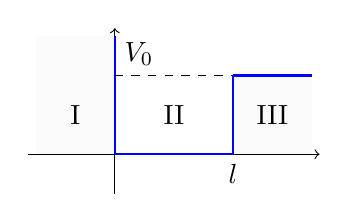
\begin{tikzpicture}[scale=0.5]
        % region
        \fill[lightgray] (-2,0) rectangle (0,3);
        \fill[lightgray] (3,0) rectangle (5,2);
        % axis
        \draw[->] (-2.2,0) -- (5.2, 0);
        \draw[->] (0,-1) -- (0, 3.2);
        % potential
        \draw[thick,blue] (0,0) -- (3,0);
        \draw[thick,blue] (0,0) -- (0,3);
        \draw[thick,blue] (3,0) -- (3,2); 
        \draw[thick,blue] (3,2) -- (5,2); 
        \draw[dashed] (0,2) -- (3,2);
        % text
        \node[] at (-1,1) {I};
        \node[] at (1.5,1) {II};
        \node[] at (4,1) {III};
    
        \node[below] at (3,0) {$l$};
        \node[above right ] at (0,2) {$V_0$};
        % functions
        % \draw[domain=-4:4,black,thick,samples=100] plot (\x,{\x*\x});
    \end{tikzpicture}
    \caption{半无限深势阱}
    \label{fig:half_inf_well}
    \end{figure}
先写出薛定谔方程
\begin{equation}
    \hat H = \hat T + \hat V(x),
\end{equation}
势能依然是分段函数,
\begin{equation}
    V(x) = 
    \begin{cases}
        +\infty, \quad &x\in(-\infty, 0),\\
        0, \quad &x\in[0,l],\\
        V_0, \quad &x\in(l,\infty),
    \end{cases}
\end{equation}

对于 block I,有
\begin{align}
    (V - E)\psi(x) &= \frac{\hbar^2}{2m} \frac{\partial \psi^2(x)}{\partial x^2} \\
    \psi(x) &= \frac{\hbar^2}{2m(V - E)} \frac{\partial^2 \psi(x)}{\partial x^2} = 0
\end{align}

对于 block II, 有
\begin{align}
    -\frac{\hbar^2}{2m} \pdv[2]{x} \psi(x) = E\psi(x),
    \label{eq:half_inf_block2_seq}
\end{align}
其通解为
\begin{equation}
    \psi(x) = C_1 \ee^{\ii k_{2}x} + C_2 \ee^{-\ii k_2 x}
\end{equation}
对应两个方向不同的波,由此引入了三个参数 $\{C_1, C_2, k_2\}$。将通解代入薛定谔方程 \eqref{eq:half_inf_block2_seq},解得 $k_2$ 与能量有关,
\begin{equation}
    E = \frac{\hbar^2}{2m} k_2^2 \rightarrow k_2 = \frac{\sqrt{2mE}}{\hbar},
\end{equation}

还是利用边界条件,求出待定参数。所有边条件都是跟品优波函数性质相关。

\textbf{边界条件 1},
\begin{equation}
    \psi(0^-) = \psi(0^+) = 0,
\end{equation}
容易得到
\begin{equation}
    C_1 \ee^0 + C_2 \ee^0 = 0,
\end{equation}
即
\begin{equation}
    C_2 = - C_1,
\end{equation}
由此将待定参数消掉一个。

对于 block III,
\begin{align}
    - \frac{\hbar^2}{2m} \pdv[2]{\psi(x)}{x} + V_0 \psi(x) &= E\psi(x), \\
    (V_0 - E) \psi(x)&= \frac{\hbar^2}{2m} \pdv[2]{x} \psi{x}
\end{align}
设 $\psi(x) = \ee^{sx}$,代回有
\begin{align}
    (V_0-E) \psi(x) &= \frac{s^2\hbar^2}{2m} \psi(x)
\end{align}
得到
\begin{eqnarray}
    s^2 = \frac{2m(V_0 - E)}{\hbar^2},
\end{eqnarray}
其中 $V_0 - E$ 的正负对结果有着决定性的影响。

当 $V_0 > E$ 时,称为\boldtext{束缚态},有
\begin{eqnarray}
    s = \pm k_3, \quad k_3 = \frac{\sqrt{2m(V_0 - E)}}{\hbar}, 
\end{eqnarray}
解得
\begin{eqnarray}
    \psi(x) = C_3 \ee^{k_3 x} + C_4 \ee^{-k_3 x},
    \label{eq:half_inf_block3_wf1}
\end{eqnarray}
%2022-09-26 13:47:16  Wenbin Fan @FDU
这时的未知参数有 $\{E, C_1, C_3, C_4\}$,其中 $E$ 是横跨三个 block 的变量,决定了 $k_2$ 和 $k_3$。接下来是一样的步骤,只要是可以精确求解的体系,比如稍复杂的氢原子,即不断引入边界条件,获得量子化的结果。

在 block I 负无穷($x=-\infty$),波函数一定为 0。在 block III 正无穷的区域,波函数一定会衰减为有限值,甚至是趋于 0 的,所以假定它不为无穷大。

\textbf{边界条件 2},
\begin{eqnarray}
    \psi(+\infty) = 0 
\end{eqnarray}
代入 \eqref{eq:half_inf_block3_wf1} 消掉了 $C_3$,还有三个待定参数 $\{E, C_1, C_4\}$。

\textbf{边界条件 3},在波函数 $x = l$ 的地方,左右波函数相等,
% 【引用 block II \& III 的波函数】
\begin{eqnarray}
    \psi(l^-) = \psi(l^+),
\end{eqnarray}
得到
\begin{eqnarray}
    C_1 \ee^{\ii k_2 l} - C_1 \ee^{-\ii k_2 l} = C_4 \ee^{-k_3 l}, \label{eq:half_condition_3}
\end{eqnarray}
还有两个待定参数。

边界条件 4,在 $x=l$ 的地方,左右波函数对坐标的偏导相等,
\begin{eqnarray}
    C_1 \ii k_2 \left[
        \ee^{\ii k_2 l} + \ee^{-\ii k_2 l} 
    \right] = - C_4 k_3 \ee^{-k_3 l} \label{eq:half_condition_4}
\end{eqnarray}
目前只剩能量 $E$ 待求。

依然使用欧拉方程,将 \eqref{eq:half_condition_3} \eqref{eq:half_condition_4} 展开成
\begin{align}
    & 2\ii \,C_1 \sin k_2l = C_4 \ee^{-k_3 l}, \\
    & 2 k_2 \ii \, C_1 \cos k_2 l = - C_4 k_3 \ee^{-k_3 l}, 
\end{align}
% [讨论为什么这么化简]
%2022-09-26 13:58:01  Wenbin Fan @FDU
左右两边分别相除
\begin{eqnarray}
    \frac1{k_2} \tan k_2l = - \frac1{k_3}. 
    \label{eq:half_inf_k2k3_0}
\end{eqnarray}
直接得到了 $k_2$ 和 $k_3$ 的关系,这样比较简单。如果分别求出 $C_1, C_4$ 和 $k_2, k_3$ 的关系,也可以讨论。

考虑到
\begin{eqnarray}
    k_2 = \frac{\sqrt{2mE}}{\hbar}, \quad k_3 = \frac{\sqrt{2m(V_0- E)}}{\hbar}, \label{eq:half_inf_k2k3_def}
\end{eqnarray}
代回 \eqref{eq:half_inf_k2k3_0},则得到能量相关的式子
\begin{eqnarray}
    \frac{\hbar}{\sqrt{2mE}} \tan \left(
        \frac l{\hbar} \sqrt{2mE}
    \right)
    = - \frac{\hbar}{2m(V_0 - E)},
    \label{eq:half_inf_k2k3_transcendental}
\end{eqnarray}
这是关于 $E$ 的超越方程,有数值解。

化简 \eqref{eq:half_inf_k2k3_transcendental},以便讨论。设
\begin{eqnarray}
    z = \frac{l}{\hbar} \sqrt{2mE}, \quad z_0 = \frac {l}{\hbar} \sqrt{2m V_0},\label{eq:half_inf_zz0_def}
\end{eqnarray}
可得
\begin{align}
    z_0^2 - z^2 &= \frac{l^2}{\hbar^2} 2m (V_0 - E),\\
    \sqrt{z_0^2 - z^2} &= \frac{l}{\hbar} \sqrt{2m (V_0 - E)},
\end{align}
所以 \eqref{eq:half_inf_k2k3_transcendental} 为
\begin{eqnarray}
    \frac{l}{z} \tan z = -\frac{l}{\sqrt{z_0^2 - z^2}},
\end{eqnarray}
将 $z$ 翻上去,有
\begin{eqnarray}
    \frac{z}{l} \cot z = -\frac{\sqrt{z_0^2 - z^2}}{l},
\end{eqnarray}
简单化简可得
\begin{eqnarray}
    \cot z = - \sqrt{\left(\frac{z_0}{z}\right)^2 - 1}. 
\end{eqnarray}
\begin{lstlisting}
(* 交互操作,查看 z0 变化时解的个数 *)
Manipulate[
    Plot[{Cot[z], -Sqrt[(z0/z)^2 - 1]}, {z, 0, 10}, 
        PlotRange -> {-6, 1}], {z0, 0, 20}]
\end{lstlisting}
\begin{figure}[tp]\centering
    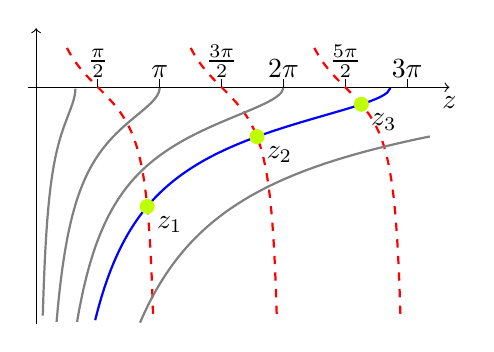
\begin{tikzpicture}[scale=0.5]
        % % region
        % \fill[lightgray] (-2,0) rectangle (0,3);
        % \fill[lightgray] (3,0) rectangle (5,2);
        % axis
        \draw[->] (-0.2,0) -- (10.5, 0);
        \draw[->] (0,-6) -- (0, 1.5);
        % text
        % \node[right] at (0,2) {I};
        \node[below] at (10.5,0) {$z$};
    
        \draw (pi/2,0) -- (pi/2,0.2);
        \node[above] at (pi/2,0) {$\frac{\pi}2$};
        \draw (pi,0) -- (pi,0.2);
        \node[above] at (pi,0) {$\pi$};
    
        \draw (3*pi/2,0) -- (3*pi/2,0.2);
        \node[above] at (3*pi/2,0) {$\frac{3\pi}2$};
        \draw (2*pi,0) -- (2*pi,0.2);
        \node[above] at (2*pi,0) {$2\pi$};
    
        \draw (5*pi/2,0) -- (5*pi/2,0.2);
        \node[above] at (5*pi/2,0) {$\frac{5\pi}2$};
        \draw (3*pi,0) -- (3*pi,0.2);
        \node[above] at (3*pi,0) {$3\pi$};
        % \node[above right ] at (0,2) {$V_0$};
        % functions
        \draw[domain=pi/4:pi-0.17,red,thick,dashed,samples=100] plot (\x,{cot(deg(\x))});
        \draw[domain=pi+pi/4:2*pi-0.17,red,thick,dashed,samples=100] plot (\x,{cot(deg(\x))});
        \draw[domain=2*pi+pi/4:3*pi-0.17,red,thick,dashed,samples=100] plot (\x,{cot(deg(\x))});
        
        \draw[domain=1.5:9,blue,thick,samples=100] plot (\x,{-sqrt(81/(\x*\x) - 1)});
        \draw[domain=0.17:1,gray,thick,samples=100] plot (\x,{-sqrt(1/(\x*\x) - 1)});
        \draw[domain=0.52:pi,gray,thick,samples=100] plot (\x,{-sqrt(pi*pi/(\x*\x) - 1)});
        \draw[domain=1.04:2*pi,gray,thick,samples=100] plot (\x,{-sqrt(4*pi*pi/(\x*\x) - 1)});
        \draw[domain=2.64:10,gray,thick,samples=100] plot (\x,{-sqrt(16*16/(\x*\x) - 1)});

        % roots
        \fill[draw, lime] (2.82259, -3.02769) circle[radius=5pt];
        \fill[draw, lime] (5.61016, -1.25442) circle[radius=5pt];
        \fill[draw, lime] (8.26182, -0.43206) circle[radius=5pt];
    
        \node[below right] at (2.82259, -3.02769) {$z_1$};
        \node[below right] at (5.61016, -1.25442) {$z_2$};
        \node[below right] at (8.26182, -0.43206) {$z_3$};
        
    \end{tikzpicture}
    \caption{半无限深势阱的解}
\end{figure}
当 $z_0 = 9$ 时,那么 $z$ 的取值是 $[0, z_0]$,画出图来看到只有 3 个解。对应于 3 个分离的束缚态 $E_i (i = 1, 2, 3)$,
\begin{eqnarray}
    E_i = \frac{\hbar^2 z^2}{2ml^2}, \quad i = 1, \cdots, N
\end{eqnarray}

最终给出半无限深势阱的波函数,
\begin{align}
    \psi_i (x) = 
    \begin{cases}
        0, \quad &x\in (-\infty, 0), \\
        C_1 \ee^{\ii k_2 x} - C_1 \ee^{-\ii k_2 x}, \quad &x\in[0,l],\\
        C_4 \ee^{-k_3 x}, \quad & x\in(l, \infty),
    \end{cases}
\end{align}
%2022-09-26 14:12:50  Wenbin Fan @FDU
% 将 $E_i$ 代入边界条件3中,得到
% \begin{align}
%     C_1 (\ee^{\ii k_2 l} - \ee^{-\ii k_2 l}) &= C_4 \ee^{-k_3 l}
% \end{align}
再给出\textbf{边界条件 5},波函数归一化
\begin{eqnarray}
    \intinf \psi^* \psi \, \dd x = 1,
\end{eqnarray}
由边界条件 3 \eqref{eq:half_condition_3} 和上式便可确定 $\{C_1, C_4\}$。边条件 3 中解得
\begin{equation}
    C_4 = C_1 \, 2\ii \,\ee^{k_3 l} \sin k_2 l,
\end{equation}
\begin{lstlisting}
Solve[Subscript[C, 1] (Exp[I k2 l] - Exp[-I k2 l]) == 
    Subscript[C, 4] Exp[-k3 l], Subscript[C, 4]] // 
  ExpToTrig // FullSimplify
>> {{Subscript[C, 4] -> 
   2 I E^(k3 l) Sin[k2 l] Subscript[C, 1]}}
\end{lstlisting}
由归一化条件可解得,
\begin{equation}
    C_1 = -\frac{\ii}2\left(
        \frac l2 + \frac1{2 k_3} \sin^2 k_2 l + \frac1{k_2} \sin 2k_2 l
    \right)^{-1/2}. 
\end{equation}
\begin{lstlisting}
res = Integrate[
    Subscript[C, 1] 2 I Sin[k2 x] Subscript[C, 1] 2 (- I) Sin[
        k2 x], {x, 0, l}] + 
    Integrate[
    2 I E^(k3 l) Sin[k2 l] Subscript[C, 1] Exp[-k3 x] 2 (-I) E^(k3 l)
        Sin[k2 l] Subscript[C, 1] Exp[-k3 x], {x, l, Infinity}, 
    Assumptions -> {k3 > 0}]
Solve[res == 1, Subscript[C, 1]] // FullSimplify
(* 运行结果略 *)
\end{lstlisting}

从以上 5 个边界条件,能给出量子化的条件。对于给定的 $z_0$ 能给出束缚态的解。

特别地,当 $z_0 < \pi/2$ 时,波函数将无解,不再有束缚态。不是只要有能垒就能束缚住电子。

% 2022-09-26 14:25:09  Wenbin Fan @FDU
% 第四节课
% 【画出波函数的图,拍照,黑、红、绿】

\boldtext{散射态}  $E > V_0$,解得
\begin{eqnarray}
    s^2 = \frac{(V_0 - E) 2 m}{\hbar^2} \rightarrow s = \pm \frac{\ii \sqrt{2m(E- V_0)}}{\hbar},
\end{eqnarray}
即
\begin{eqnarray}
    \psi(x) = C_3 \ee^{\ii k_3 x} + C_4 \ee^{-\ii k_3 x}, \quad k_3 = \frac{\ii\sqrt{2m(E-V_0)}}{\hbar},
\end{eqnarray}
这里有虚数,所以不能用无穷大的边界条件了。

\textbf{边界条件 3},
\begin{eqnarray}
    \psi(l^-) = \psi(l^+),
\end{eqnarray}
即
\begin{eqnarray}
    C_1 (\ee^{\ii k_2 l} - \ee^{-\ii k_2 l}) = 
    C_3 \ee^{\ii k_3 l} + C_4 \ee^{-\ii k_3 l}
\end{eqnarray}
\textbf{边界条件 4},
\begin{eqnarray}
    \psi'(l^-) = \psi'(l^+)
\end{eqnarray}
% 【检查上面的边界条件有没有 prime】
即
\begin{eqnarray}
    C_1 \ii k_2 (\ee^{\ii k_2 l} + \ee^{\ii k_2 l}) = \ii k_3 (C_3 \ee^{\ii k_3 l} - C_4 \ee^{-\ii k_3 l} )
\end{eqnarray}
省略推导过程,可以解出来
\begin{align}
    &C_3 = \frac12 \left[
        \left(1 + \frac{k_2}{k_3}\right) \ee^{\ii k_2 l} - 
        \left(1 - \frac{k_2}{k_3}\right) \ee^{-\ii k_2 l}
    \right] \ee^{-\ii k_3 l }C_1, \label{eq:half_inf_scat_c3}\\
    &C_4 = \frac12 \left[
        \left(1 - \frac{k_2}{k_3}\right) \ee^{\ii k_2 l} - 
        \left(1 + \frac{k_2}{k_3}\right) \ee^{-\ii k_2 l}
    \right] \ee^{\ii k_3 l} C_1, \label{eq:half_inf_scat_c4}
\end{align}
\begin{lstlisting}
Clear["Global`*"]
Solve[{Subscript[C, 1] (Exp[I k2 l] - Exp[-I k2 l]) == 
    Subscript[C, 3] Exp[I k3 l] + Subscript[C, 4] Exp[-I k3 l], 
    Subscript[C, 1] k2 (Exp[I k2 l] + Exp[-I k2 l]) == 
    k3 (Subscript[C, 3] Exp[I k3 l] - 
        Subscript[C, 4] Exp[-I k3 l])}, {Subscript[C, 3], 
    Subscript[C, 4]}] // FullSimplify
>> {{Subscript[C, 3] -> (
    E^(-I k3 l) (k2 Cos[k2 l] + I k3 Sin[k2 l]) Subscript[C, 1])/k3, 
    Subscript[C, 4] -> (
    E^(I k3 l) (-k2 Cos[k2 l] + I k3 Sin[k2 l]) Subscript[C, 1])/k3}}
\end{lstlisting}
%2022-09-26 14:34:13  Wenbin Fan @FDU

有几个结论,
(1) 注意到 $C_3^* = C_4$,可以知道 $\psi(x)$ 在 block III 是实三角函数,
(2) $k_2$ 与 $k_3(E)$ 没有任何限制要求,即本征值无限多,散射态是连续谱。因为没有其它可用的边界条件了,所以没有了量子化的能级。尽管这有点违背直觉。

\homework{
    \textbf{3.4}
    (1) 利用公式 \eqref{eq:half_inf_scat_c4},求
    $|C_1|^2$ 与 $|C_3|^2$ 
     的关系,并比较二者大小。
}

散射态的方程为
\begin{eqnarray}
    \phi (x) = \begin{cases}
        0, \quad &x \in (-\infty, 0), \\
        C_1 \ee^{\ii k_2 x} - C_1 \ee^{-\ii k_2 x}, \quad &x \in [0,l], \\
        C_3 \ee^{\ii k_3 x} + C_4 \ee^{-\ii k_3 x}, \quad &x \in (l, \infty),
    \end{cases}
\end{eqnarray}
直觉上来理解,$|C_1|^2$ 是粒子散射态反射回来的概率,$|C_3|^2$ 是投射过去的概率。

\homework{
    \textbf{3.4} (2) 推导并画出 $z = 12$, $z_0 = 9$ 时的体系波函数。
}

\section{阶梯势垒体系}
\begin{figure}[tp]\centering
    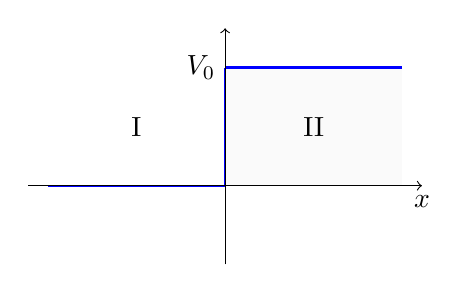
\begin{tikzpicture}[scale=0.5]
        % region
        % \fill[lightgray] (-5,0) rectangle (0,4);
        \fill[lightgray] (0,0) rectangle (4.5,3);
        \draw[blue,thick] (-4.5,0) -- (0,0);
        \draw[blue,thick] (0,0) -- (0,3);
        \draw[blue,thick] (0,3) -- (4.5,3);
        % axis
        \draw[->] (-5,0) -- (5, 0);
        \draw[->] (0,-2) -- (0, 4);
        % text
        \node[below] at (5,0) {$x$};
        \node[left] at (0,3) {$V_0$};
        \node at (-2.25, 1.5) {I};
        \node at (2.25, 1.5) {II};
    \end{tikzpicture}
\caption{阶梯势垒}
\end{figure}
\begin{eqnarray}
    V(x) = 
\begin{cases}
    0, \quad x\in(-\infty, 0), \\
    V_0, \quad x\in[0, \infty],
\end{cases}
\end{eqnarray}

对于 block I, 解出
\begin{eqnarray}
    \psi(x) = C_1 \ee^{\ii k_1 x} + C_2 \ee^{- \ii k_2 x},
\end{eqnarray}
其中
\begin{eqnarray}
    k_1 = \frac{\sqrt{2mE}}{\hbar}
\end{eqnarray}
有三个待定参数 $\{C_1, C_2, E\}$。

对于 block II,与单侧无限深势阱中的 block III 是一致的。
% 【直接复制过来上面的求解,已拍照】
%2022-09-26 14:46:05  Wenbin Fan @FDU

\boldtext{散射态} $E > V_0$,推出
\begin{eqnarray}
    S = \pm \ii k_2, \quad k_2 = \frac{\sqrt{2m(E-V_0)}}{\hbar}
\end{eqnarray}
波函数
\begin{align}
    \psi(x) = \begin{cases}
        C_1 \ee^{\ii k_1 x} + C_2 \ee^{\ii k_1 x},\quad & x \in (-\infty, 0), \\
        C_3 \ee^{\ii k_2 x} + C_4 \ee^{\ii k_2 x}, \quad & x \in [0, \infty),
    \end{cases}
\end{align}
有 5 个待定参数 $\{C_1, C_2, C_3, C_4, E\}$。

% 【画图】
多个动量本征态的叠加。
% $C_1$ $C_3$ 都是向右方向的动量本征矢。
\begin{figure}[tp]\centering
    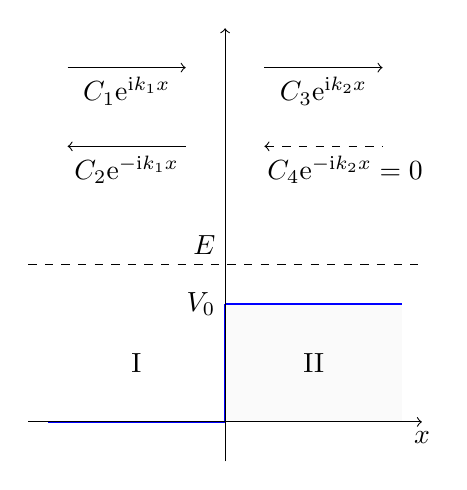
\begin{tikzpicture}[scale=0.5]
        % region
        % \fill[lightgray] (-5,0) rectangle (0,4);
        \fill[lightgray] (0,0) rectangle (4.5,3);
        \draw[blue,thick] (-4.5,0) -- (0,0);
        \draw[blue,thick] (0,0) -- (0,3);
        \draw[blue,thick] (0,3) -- (4.5,3);
        % axis
        \draw[->] (-5,0) -- (5, 0);
        \draw[->] (0,-1) -- (0, 10);
        % text
        \node[below] at (5,0) {$x$};
        \node[left] at (0,3) {$V_0$};
        \node at (-2.25, 1.5) {I};
        \node at (2.25, 1.5) {II};
        %
        \draw[dashed] (-5, 4) -- (5, 4);
        \node[above left] at (0,4) {$E$};
        %
        \draw[->] (-4,9) -- (-1,9);
        \node[below] at (-2.5, 9) {$C_1 \mathrm{e}^{\mathrm ik_1 x}$};
        \draw[<-] (-4,7) -- (-1,7);
        \node[below] at (-2.5, 7) {$C_2 \mathrm{e}^{-\mathrm ik_1 x}$};
        \draw[->] (1,9) -- (4,9);
        \node[below] at (2.5, 9) {$C_3 \mathrm{e}^{\mathrm ik_2 x}$};
        \draw[<-,dashed] (1,7) -- (4,7);
        \node[below] at (2.5, 7) {$\phantom{0=}C_4 \mathrm{e}^{-\mathrm ik_2 x} = 0$};
    
        % functions
        % \draw[domain=pi/4:pi-0.17,red,thick,dashed,samples=100] plot (\x,{cot(deg(\x))});
    \end{tikzpicture}
    \caption{波的方向示意图}
\end{figure}

概率流密度的定义
\begin{eqnarray}
    J = \frac{\ii\hbar}{2m} \left[
        \psi^* \pdv[x] \psi - \psi \pdv[x] \psi^*
    \right]
\end{eqnarray}
对于 block I,
\begin{eqnarray}
    J_1 = \frac{k_1 \hbar}{m} \left(
        |C_1|^2 - |C_2|^2
    \right)
\end{eqnarray}
这个体系中的截面只有一条线,流入为负,流出为正,因此
$\frac{k_1 \hbar}{m} |C_1|^2$ 为进入 block I 入射波($C_1 \ee^{-\ii k_1 x}$)的概率流密度,
同理 $\frac{k_1 \hbar}{m} |C_2|^2$ 为反射波($C_2 \ee^{-\ii k_2 x}$)的概率流密度,因此可得 $\frac{k_2 \hbar}{m} |C_3|^2$ 为进入 block III 的波($C_3 \ee^{\ii k_3 x}$)的概率流密度,特别地,$\frac{k_2 \hbar}{m} |C_4|^2 = 0$,因为不会有反射回来的波,所以 $C_4 = 0$。

思考,一个能量为 $E$($E>V_0$)的粒子从 $\infty$ 向 $-\infty$ 传播,此时边界条件 3
\begin{eqnarray}
    \psi(0^-) = \psi(0^+),
\end{eqnarray}
推出
\begin{eqnarray}
    C_1 + C_2 = C_3,
\end{eqnarray}
边界条件 4
\begin{eqnarray}
    \psi'(0^-) = \psi'(0^+)
\end{eqnarray}
推出
\begin{eqnarray}
    k_1 (C_1 - C_2) = k_2 C_3,
\end{eqnarray}
联立解得
% 【见照片,有 ref】
%2022-09-26 15:02:08  Wenbin Fan @FDU
% 【k1 k2 def】【没拍全】
\begin{align}
    & C_2 = \frac{k_1 - k_2} {k_1 + k_2} C_1, \\
    & C_3 = \frac{k_1}{k_1 + k_2} C_1,
\end{align}

定义反射系数
\begin{eqnarray}
    R = \frac{ \displaystyle \frac{k_1 h}m |C_2|^2 } { \displaystyle \frac{k_1 h}m |C_1|^2 } = \frac{(k_1 - k_2)^2} {(k_1 + k_2)^2}, 
\end{eqnarray}
定义透射系数,
\begin{eqnarray}
    T = \frac{ \displaystyle \frac{k_2 h}m |C_2|^2 } { \displaystyle \frac{k_1 h}m |C_1|^2 } = \frac{4k_1k_2} {(k_1 + k_2)^2}, 
\end{eqnarray}
显然有 $R^2 + T^2 = 1$。

代入 $k_1, k_2$ 的定义
\begin{eqnarray}
    R = \left( 1 - \sqrt{1 - \frac{V_0}E}\right)^2 
    \left( 1 + \sqrt{1 - \frac{V_0}E}\right)^{-2},
\end{eqnarray}
当 $0 < \frac{V_0}{E} < 1$ 时,
% 【画图 R - (V0/E) 的图,类似 $x^2$ 的图】
哪怕到了 $\frac{V_0}E = 80\%$,透射率只有 15\%,当 $E = V_0$ 时全反射,并不是像想象中的那样越过去。
\begin{lstlisting}
(* 画出 R-(V0/E) 的图 *)
Plot[(-1 + Sqrt[1 - x])^2/(1 + Sqrt[1 - x])^2, {x, 0, 1}, 
    PlotRange -> {0, 1}]
\end{lstlisting}

\section{有限高方势垒}
\begin{figure}[tp]\centering
    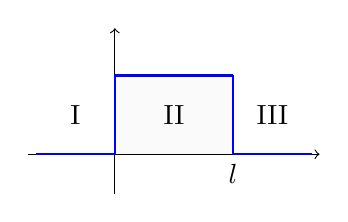
\begin{tikzpicture}[scale=0.5]
        % \fill[lightgray] (-2,0) rectangle (0,3);
        \fill[lightgray] (0,0) rectangle (3,2);
        % axis
        \draw[->] (-2.2,0) -- (5.2, 0);
        \draw[->] (0,-1) -- (0, 3.2);
        % potential
        \draw[thick,blue] (-2,0) -- (0,0);
        \draw[thick,blue] (0,0) -- (0,2);
        \draw[thick,blue] (0,2) -- (3,2);
        \draw[thick,blue] (3,0) -- (3,2); 
        \draw[thick,blue] (3,0) -- (5,0);
        % text
        \node[] at (-1,1) {I};
        \node[] at (1.5,1) {II};
        \node[] at (4,1) {III};
        
        \node[below] at (3,0) {$l$};
        % functions
        % \draw[domain=pi/4:pi-0.17,red,thick,dashed,samples=100] plot (\x,{cot(deg(\x))});
    \end{tikzpicture}
    \caption{有限高方势垒}
    \end{figure}
势能的形式,
\begin{eqnarray}
    V(x) = 
        \begin{cases}
            0, \quad &x \in (-\infty,0),\\
            V_0, \quad &x \in[0,l],\\
            0, \quad &x \in (l, \infty),
        \end{cases}
\end{eqnarray}

分情况讨论,$E<V_0$ 时,得到波函数
\begin{eqnarray}
    \psi(x) =
\begin{cases}
    C_1 \ee^{\ii k_1 x} + C_2 \ee^{-\ii k_1 x}, \quad &x \in (-\infty, 0), \\
    C_3 \ee^{\ii k_2 x} + C_4 \ee^{-k_2 x}, \quad &x \in[0,l],\\
    C_5 \ee^{\ii k_3 x}, \quad &x \in(l, \infty),
\end{cases}
\end{eqnarray}
\homework{
    \textbf{3.5} 求出有限高方势垒($E<V_0$)的波函数。
}
% 
\section{复习}
\chat{%
国庆少了一节课。前面三次课回顾了历史、量子力学的公设、简单的一维体系。
}
\courseTime{Oct. 10, 2022\\Week 6\\4th}

量子力学公设,

1. 微观体系均可用含时的品优波函数描述,品优指单值连续有限,品优也是很多解的物理源头。

2. 任何可观测的力学量都对应线性算符,等于平均值。
\begin{eqnarray}
    \langle\hat{F}\rangle=\int_{-\infty}^{+\infty} \varphi^* \hat{F} \varphi d \tau=\langle\varphi|\hat{F}| \varphi\rangle
\end{eqnarray}

3. 一个算符作用到任何一个状态波函数,等于常数乘波函数,称这个波函数是本征函数。任何任意一个线性的厄米算符,那本征方程是
\begin{equation}
    \hat F \psi_i = \lambda_i \psi_i,
\end{equation}
并且它的本征函数构成完备集 $\{\psi_i\}$

4. 如果这个本征方程是厄米算符的本征方程,那么它有正交归一的性质,
\begin{align}
    \langle\psi_i | \psi_j \rangle = \delta_{ij} = \begin{cases}
        1, \quad &i = j, \\
        0, \quad &i\neq j,
    \end{cases}
\end{align}

% 4. 厄米算符有正交归一的性质
% \begin{eqnarray}
%     \hat F \psi_i = \lambda_i \psi_i, 
% \end{eqnarray}

\chat{%
从这个量子力学公设出发,我们可以知道量子化学里最重要的一个定态方程——薛定谔定态方程 $\hat H \psi_i = E_i \psi_i$。它是哈密顿算符的本征函数,哈密顿算符包含了动能项跟势能项,
\begin{eqnarray}
    \hat H = \hat T + \hat V = - \frac{\hbar^2}{2m}\pdv[2]{x} + \hat V
\end{eqnarray}
其中,对于单电子体系,动能算符是系统无依赖的算符。
但是体系的不同完全是由势能算符来给定的,所以不同的势能就对应的不同的体系。

在上一周课,我们讲了一维的量子体系。如果我们想要了解一个微观体系的信息,我们首先必须给出这个量子体系的薛定谔方程,这就是量子力学体系的状态波函数。对于量子力学的状态波函数的求解,需要通过定态许欸那个方程。而定态薛定谔方程的构建,最重要的一点就是对于势函数的构建。所以不同的量子力学体系,本质上就对应于不同的势函数以及势函数所对应的边界条件。}

最简单的一维量子力学体系,就是所谓的无限深势阱,如图 \ref{fig:inf_well}。
% 上周讲了一维的量子体系,
% 【】
% 必须给出状态波函数。通过定态薛定谔方程构建,关键就是势能函数、边界条件。最简单的一维量子体系是一维无线深势阱,【图】
\begin{align}
    V(x) = 
    \begin{cases}
        0, \quad &x\in[0,l],\\
        +\infty, \quad &\text{other}
    \end{cases}
\end{align}
能量 \begin{align}
    E_i = \frac{\hbar^2\pi^2 i^2} {2ml^2}, i = 1,2,3,\cdots,
\end{align}能得到零点能。

上周还讲了单侧无限深势阱,其一侧是无穷大,另一侧是有限的 $V_0$,如图 \ref{fig:half_inf_well}。这个体系的波函数比无限深势阱更复杂一些,势能表达式为
\begin{align}
    V(x) = 
    \begin{cases}
        \infty, \quad & x \in (-\infty, 0),\\
        0, \quad&x \in [0,l],\\
        V_0, \quad &\text{其它},
    \end{cases}
\end{align}
其能量满足的是
\begin{align}
    \cot z = -\sqrt{\left( \frac{z_0}z \right)^2 - 1}
\end{align}
超越方程,其中
\begin{align}
    z = \frac l\hbar \sqrt{2 m E}, \quad z_0 = \frac{l}{\hbar} \sqrt{2mV_0},
\end{align}
通过求解这个超越方程,能给出能量的量子化。$\{z_i\}$ 是量子化的,可求出能量 $E_i = \frac{\hbar^2 z_i^2}{2ml^2}$。

这个超越方程的形状、求解,上周有讲过。它的右边,当 $z \rightarrow0$ 时是无穷大,并且截止到 $z_0$,左边是 $\cot$ 函数,周期为 $\pi$,左右两边函数的交点就是解。当 $z_0 < \frac{\pi}2$ 时,没有交点,没有解,此时无法束缚。我们知道 $z_0$ 与 $V_0$ 有关,也就是当 $V_0$ 足够小的时候,是不能束缚住粒子的。当 $z_0 = \frac{\pi}2$ 时,系统可以束缚住粒子,此时解为 $z_1 = \frac{\pi}2$。当 $z_0 \geqslant \frac{\pi}2$ 时才有解,
\begin{align}
    z_0 = \frac{l}{\hbar} &\geqslant \frac{\pi}2 \\
    \frac{l^2}{\hbar^2} 2 m V_0 &\geqslant \frac{pi^2}4 \\
    V_0 &\geqslant \frac14 \frac{\hbar^2\pi^2}{2ml^2},
\end{align}
最小的束缚态能量为零点能的 1/4,即
\begin{align}
    V_0^{\text{min}} = \frac14 E_1,
\end{align}

\begin{figure}[tp]\centering
    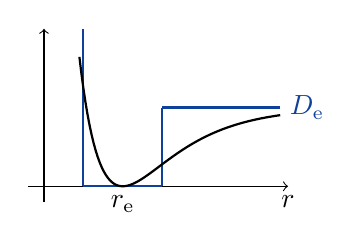
\begin{tikzpicture}[scale=1.0]
        % axis
        \draw[->] (-0.2,0) -- (3.1, 0);
        \draw[->] (0,-0.2) -- (0, 2);
        \node[below] at (3.1,0) {$r$};
        % \fill[lightgray] (-2,0) rectangle (0,3);
        % \fill[lightgray] (0,0) rectangle (3,2);
        % % potential
    
        \draw[thick,fudanBlue] (0.5,0) -- (0.5,2);
        \draw[thick,fudanBlue] (0.5,0) -- (1.5,0);
        \draw[thick,fudanBlue] (1.5,0) -- (1.5,1);
        \draw[thick,fudanBlue] (1.5,1) -- (3.0,1);
        
        % \node[below] at (3,0) {$l$};
        % functions
        \draw[domain=0.45:3,thick,samples=100] plot (\x,{(1 - exp(-1.5* (\x - 1)))^2});
        \node[below] at (1.0,0) {$r_{\mathrm e}$};
        \node[right,fudanBlue] at (3.0,1) {$D_{\mathrm e}$};
    
    \end{tikzpicture}
    \caption{分子间势能与半无限深势垒}
\end{figure}
这个半无限深的模型体系有什么用呢?可以类比化学键的行为。以氢气为例,
\begin{align}
    \text{键能} \quad &D_{\mathrm e} = \SI{4.74}{\electronvolt}\\
    \text{零点能} \quad &\SI{0.26}{\electronvolt}\\
    \text{平衡位置} \quad &r_{\mathrm e} = \SI{0.7414}{\angstrom}
\end{align}把氢气用这个半无限深势阱描述,其中单位换算为
\begin{align}
    & m = \SI{1.673E-27}{\kilo\gram}, \quad \mu = \frac{m}2, \\
    & \hbar = \SI{1.055E-34}{\joule\second},\\
    & \SI{1}{\electronvolt} = \SI{1.602E-19}{\joule},
\end{align}
这里的 $\mu$ 是氢分子的折合质量,满足
\begin{align}
    \frac1\mu = \frac1{m_{\mathrm H}} + \frac1{m_{\mathrm H}}, 
\end{align}
代入数据,得到
\begin{align}
    z_0 &= \frac{l}{\hbar} \sqrt{2 m V_0} \notag\\
    &= \frac{\SI{0.5E-10}{\metre}}{\SI{1.055E-34}{\joule\second}} \sqrt{
        \SI{1.673E-27}{\kilo\gram} \times 
        \SI{4.74}{\electronvolt} \times
        \SI{1.602E-19}{\joule\per\electronvolt}
    } \notag\\
    &\approx 23.89 \approx 7.6 \pi,
\end{align}
当 $z_0$ 很大时,$z_1$ 接近于 $\pi$,也就是接近于无限深势阱的 $z_1$。

应用量子化条件,得到零点能
\begin{equation}
    E_1 = \frac{\hbar^2\pi^2}{2ml^2} = \SI{0.04}{\electronvolt},
\end{equation}
求解出来发现这个模型并不能很好描述化学键。

\chat{%
氢气分子在平衡位置附近是连续的,目前这里的阶跃势能是有碍于正确描述零点能的。很自然的想法是用抛物线势能描述势能,本周主要的内容便是量子谐振子。
}
%2022-10-10 08:32:51  Wenbin Fan @FDU
\chapter{量子谐振子}
% 【图】【二次函数】
\begin{figure}[tp]\centering
    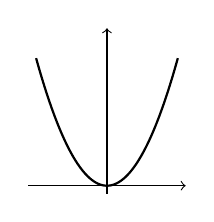
\begin{tikzpicture}[scale=0.5]
        % axis
        \draw[->] (-2,0) -- (2, 0);
        \draw[->] (0,-0.2) -- (0, 4);
        % \node[below] at (3.1,0) {$r$};
    
        \draw[domain=-1.8:1.8,thick,samples=100] plot (\x,{\x*\x});
    
    \end{tikzpicture}
    \caption{抛物势}
\end{figure}
势函数
\begin{align}
    V(x) = a x^2,
\end{align}
称为\boldtext{抛物线} parabolic 势函数。
% 【刚才是???,有什么不一样】
% 【求得波函数???】
\chat{%
刚才通过化学键的定义,引出了量子体系。换个角度,量子谐振子有什么不同?我们能从公设推知微观粒子的行为,前提是确立状态方程、求解波函数,其中状态方程中最重要的系统依赖项就是势函数。上周的一维量子体系是简单的量子状态,要么为 0,要么是有限值,所有的复杂情况都来自边界条件,由边条件可以推知所有的物理。

今天要求解的量子体系,势函数是显式地依赖于坐标的。求解之前有个问题,$a$ 表示的是什么物理量。
}
\begin{figure}[tp]\centering
    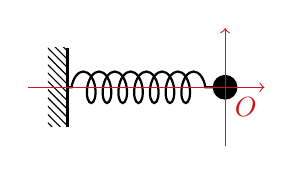
\begin{tikzpicture}[scale=0.5]
        % % axis
        % \draw[->] (-2,0) -- (2, 0);
        % \draw[->] (0,-0.2) -- (0, 4);
        % % \node[below] at (3.1,0) {$r$};
    
        \fill [pattern = north west lines] (-0.5,0) rectangle (0,2);
        \draw[thick] (0,0) -- (0,2);
        \draw[
        decoration={
            coil,
            segment length = 2mm,
            amplitude = 2mm,
            aspect = 0.5,
            post length = 1mm,
            pre length = 0.5mm},
        decorate, thick] (0,1) -- (4,1);
        \draw[fill] (4,1) circle (0.3);
    
        % \draw[domain=-1.8:1.8,thick,samples=100] plot (\x,{\x*\x});
    
        % axis
        \draw[->, fudanRed] (-1,1) -- (5, 1);
        \draw[->, fudanRed] (4,-0.5) -- (4, 2.5);
        \node[right,fudanRed] at (4,0.5) {$O$};
    
    \end{tikzpicture}
    \caption{弹簧模型}
    \end{figure}
回顾胡克定理,
% 【图,左边是墙,水平连接弹簧】,
以平衡构型建立坐标系 $O$,弹簧受到的力为 $F = -kx$,$k$ 是弹簧的劲度系数 stiffness coefficient。由牛顿力学定律
\begin{align}
    F = ma = m \pdv[2]{x}{t} = -k x
\end{align}
得到偏微分方程
\begin{align}
    \pdv[2]{x}{t} = - \frac km x,
\end{align}
很容易得到运动轨迹
\begin{align}
    x(t) = A \sin(\omega t + \delta),
\end{align}
其中 $\omega = \sqrt{\frac{k}m}$ 是振子的角频率,是体系内禀的量,$A,\delta$ 是振幅和相位,与初态有关。另外我们知道,
\begin{align}
    F(x) = -\frac{\partial V(x)}{\partial x}, 
\end{align}
解出来势能
\begin{align}
    V(x) = \int -F(x)\,\dd x = \int kx \, \dd x = \frac12 k x^2 + V_0,
\end{align}
令参考势能 $V_0 = 0$,那么势能
\begin{eqnarray}
    V(x) = \frac 12 kx^2 = \frac 12 m\omega^2 x^2.
\end{eqnarray}
由此,得到了 $a$ 的物理含义。

量子谐振子的哈密顿量,
\begin{align}
    \hat H(x) = -\frac{\hbar^2}{2m} \pdv[2]{x} + \frac 12 m\omega^2 x^2,
\end{align}
定态薛定谔方程就可以写为
\begin{align}
    -\frac{\hbar^2}{2m} \pdv[2]{\psi}{x} + \frac 12 m\omega^2 x^2 = E\psi,
    \label{eq:harm_seq_original}
\end{align}
看起来有点太复杂了,能否简化其中的常数?

\section{方程简化}

两边同除以 $-\frac{\hbar^2}{2m}$,
\begin{align}
    \pdv[2]{\psi}{x} - \frac{m^2\omega^2 x^2}{\hbar^2} \psi = \frac{-2mE}{\hbar^2}\psi,
\end{align}
归并到左边,有
\begin{align}
    \pdv[2]{\psi(x)}{x} + \left(
        \frac{2mE}{\hbar^2} - \frac{m^2\omega^2}{\hbar^2} x^2
    \right) \psi = 0,
\end{align}
设 $a = \frac{m\omega}{\hbar}$,有
\begin{align}
    \pdv[2]{\psi(x)}{x} + \left(
        \frac{2mE}{\hbar^2} - a^2 x^2
    \right) \psi = 0,
    \label{eq:harm_seq_a}
\end{align}
利用函数变量代换的规则,定义新的变量 $y = kx$,即 $x = \frac 1k y$,那么波函数 $\psi(x) = \psi(y)$,利用链式法则
\begin{align}
    &\pdv{\psi(x)}{x} = \pdv{\psi(y)}{y} \pdv yx = k \pdv{\psi(y)} {y},
    &\pdv[2]{\psi(x)}{x} = k^2 \pdv[2]{\psi(y)}{y},
\end{align}
代回薛定谔方程 \eqref{eq:harm_seq_a}
\begin{align}
    k^2 \pdv[2]{\psi(y)}{y} + \left(
        \frac{2mE}{\hbar^2} - \frac{a^2}{k^2} y^2
    \right) \psi(y) &= 0 \\
    \pdv[2]{\psi(y)}{y} + \left(
        \frac{2mE}{\hbar^2} - \frac{a^2}{k^4} y^2
    \right) \psi(y) &= 0
\end{align}
之前对 $k$ 是没有要求的,这里为了化简系数,令 $y^2$ 项前的系数为 1,设 $k^4 = a^2$,有 $y = \sqrt a x$,得到
\begin{align}
    \pdv[2]{\psi(y)}{y} + \left(
        \frac{2mE}{\hbar^2} - y^2
    \right) \psi(y) &= 0
\end{align}
其中还有一项
\begin{eqnarray}
    \frac{2mE}{a\hbar^2} = \frac{2mE}{m\omega\hbar^2} = \frac{2E}{\hbar\omega} = \lambda,
\end{eqnarray}
有
\begin{align}
    \pdv[2]{\psi(y)}{y} + (\lambda - y^2) \psi(y) = 0,
    \label{eq:harm_seq_lambda_y}
\end{align}
% 【标记了原始 Seq (1),上式为 2】
这种偏微分方程叫做变系数二阶常微分方程,这就是谐振子的\boldtext{标准方程}。

\chat{%
这个方程有很多种解法,已经被研究得很透彻了,这里讲一个标准做法。

为了求解,有必要对这个微分方程的轮廓有认知。
首先遇到的问题,是否有对称性,或者说具有什么样的对称性?
}
% 第二节
% 【】
\section{波函数的对称性}
由势函数可知
\begin{align}
    V(x) = V(-x),
\end{align}
因此对应的本征波函数 $\psi(x)$ 即 $\psi(y)$ 有确定的宇称,那么波函数要么是奇函数 $\psi(x) = -\psi(-x)$、要么是偶函数 $\psi(x) = \psi(-x)$。
\homework{\textbf{4.1} ~ (a) 对于一维的宇称算符
\begin{align}
    \hat\Pi \psi(x) = \psi(x),
\end{align}
证明 $\hat \Pi$ 是 Hermit 算符,

(b) 证明,当 $V(x) = V(-x)$ 时,$[\hat H, \hat \Pi] = 0$,

(c) 考察 $[\hat T, \hat V]$ 是否为 0,并进一步考察 $[\hat T, \hat H]$、$[\hat V, \hat H]$ 是否为 0。
}

\section{无穷远处的渐进性质}
为了求解方程,先尝试求极限情况。

当 $x \rightarrow \pm \infty$,即 $y \rightarrow \pm \infty$,$y^2 \gg \lambda$,有
\begin{align}
    \frac{\partial^2 \varphi(y)}{\partial y^2}+\left(\lambda-y^2\right) \varphi(y)=0 \Rightarrow \frac{\partial^2 \varphi(y)}{\partial y^2}-y^2 \varphi(y)=0,
\end{align}

设 $\psi(y) = \ee^{sy}$,它非奇非偶,不满足。换一种波函数,设 $\psi(y) = \ee^{sy^2}$,如果要满足品优波函数的性质,$s<0$,所以直接设为 $\psi(y) = \ee^{-sy^2} (s>0)$,求导有
\begin{align}
    &\frac{\partial}{\partial y} \ee^{-sy^2} = -2sy \, \ee^{-sy^2}, \\
    &\pdv[2]{\psi(y)}{y} = -2 s\, \ee^{-s y^2} + 4 s^2 y^2 \ee^{-s y^2},
\end{align}
\begin{lstlisting}
    D[Exp[-s y^2], y]
    D[Exp[-s y^2], {y, 2}]
    >> -2 E^(-s y^2) s y
    >> -2 E^(-s y^2) s + 4 E^(-s y^2) s^2 y^2
    \end{lstlisting}
代回原式有
\begin{align}
    4s^2 y^2 \, \ee^{-sy^2} - y^2 \ee^{-sy^2} - 2 s \ee^{-sy^2} &= 0 \\
    4s^2 y^2 \, \ee^{-sy^2} - y^2 \ee^{-sy^2} &= 0, \\
    4 s^2 & = 1,
\end{align}
解得 $s = \frac12$。得到了波函数在无穷远处的渐进性为,
\begin{equation}
    \psi(y) |_{y \rightarrow \pm\infty} = \ee^{-y^2/2}.
\end{equation}
\section{引入 Hermite 方程}
波函数可以写为
\begin{equation}
    \psi(y) = f(y) \ee^{-y^2/2},
\end{equation}
问题转化成了求解 $f(y)$。

当$y\rightarrow\pm\infty$ 时,$f(y) \rightarrow A$ 常数,才能确保 $\psi$ 的渐进行为。重新求导 
% % []
% \begin{align}
%     \pdv[2]{\psi(y)}{y} + (\lambda - y^2) \psi(y) = 0, 
% \end{align}
% []
% \begin{align}
%     \psi(y) = f(y) \, \ee^{-y^2/2},
% \end{align}
% $f(y)$ 为待求解函数,当 $y \rightarrow \pm\infty$ 时,$f(y) = A$,$\psi(y) \rightarrow \ee^{-y^2/2}$,
% 偏导为
\begin{align}
    &\frac{\partial \varphi(y)}{\partial y}=\frac{\partial f(y) e^{-y^2/2}}{\partial y}=f(y) e^{-y^2 / 2}-y e^{-y^2 / 2} f(y) \\
    &\frac{\partial^2 \varphi(y)}{\partial y^2}=f^{\prime \prime}(y) e^{-y^2 / 2}-2 y e^{-y^2 / 2} f^{\prime}(y)+\left(y^2-1\right) e^{-y^2 / 2} f(y)
\end{align}
\begin{lstlisting}
Clear[f, y]
D[f[y] Exp[-y^2/2], y] // Simplify
D[f[y] Exp[-y^2/2], {y, 2}] // Simplify
>> E^(-(y^2/2)) (-y f[y] + Derivative[1][f][y])
>> E^(-(y^2/2)) 
    ((-1 + y^2) f[y] - 2 y Derivative[1][f][y] 
    + (f^\[Prime]\[Prime])[y])
\end{lstlisting}
代回到 \eqref{eq:harm_seq_lambda_y} 中,
\begin{align}
    f^{\prime \prime}(y) e^{-y^2 / 2}-2 y e^{-y^2 / 2} f^{\prime}(y)+(\lambda-1) e^{-y^2 / 2} f(y)=0
\end{align}
% [][]Hermite 方程。
% 【】【】【4式】
稍微化简即可得另一个变系数常微分方程,
\begin{align}
    f''(y) - 2y f'(y) + (\lambda - 1) f(y) = 0, 
    \label{eq:harm_lambda_y_simp} %eq4 in course
\end{align}
称其为 Hermite 方程。

\chat{%
回到初始薛定谔方程,引入变量代换可以得到变系数常微分方程。很自然的问题是,
为什么我们要做如此多步的方程演化?换句话说,我们可否直接求 \eqref{eq:harm_seq_original} 或 \eqref{eq:harm_seq_lambda_y}?为什么变换之后求解更方便?

物化里面可能讲过,下面将会用到幂级数展开法。
}

\section{幂级数展开法}
将函数作级数展开,
\begin{align}
    &f(y) = \sum_{n=0}^\infty c_n y^n = c_0 + c_1 y + c_2 y^2 + \cdots,\\
    &f'(y) = \sum_{n=1}^\infty n c_n y^{n-1}, \\
    &f''(y) = \sum_{n=2}^\infty n(n-1) c_n y^{n-2},
\end{align}
将幂级数代回 \eqref{eq:harm_lambda_y_simp},
% 【label 5,6】
% 代回【?】,
导数的下限取值从 1、2 开始,写成从 0 开始是完全一样的,
\begin{align}
    & \sum_{n=2}^{\infty} n(n-1) c_n y^{n-2}-2 y \sum_{n=1}^{\infty} n c_n y^{n-1}+(\lambda-1) \sum_{n=0}^{\infty} c_n y^n \\
    =& \sum_{n=2}^n n(n-1) c_n y^{n-2}-\sum_{n=1}^{\infty} 2 n c_n y^n+\sum_{n=0}^{\infty}(\lambda-1) c_n y^n \\
    =& \sum_{n=2}^n n(n-1) c_n y^{n-2}-\sum_{n=0}^{\infty}(2 n-\lambda+1) c_n y^n
\end{align}
设 $m=n-2$,有
\begin{align}
    \sum_{m=0}^{\infty}(m+2)(m+1) c_{m+2} y^m-\sum_{n=0}^{\infty}(2 n-\lambda+1) c_n y^n
\end{align}
设 $n=m$,再把变量换回 $n$,有
\begin{align}
    &\sum_{n=0}^{\infty}(n+2)(n+1) c_{n+2} y^n-\sum_{n=0}^{\infty}(2 n-\lambda+1) c_n y^n \\
    ={}&\sum_{n=0}^{\infty}\left[(n+2)(n+1) c_{n+2}-(2 n-\lambda+1) c_n\right] y^n = 0, 
\end{align}
上式为 0,意味着其中每一项都要相等,
\begin{align}
    (n+2)(n+1) c_{n+2} = (2n - \lambda + 1)c_n,
\end{align}
便得到了双间隔的递推公式
\begin{align}
    c_{n+2} = \frac{2n - \lambda + 1}{(n+2)(n+1)} c_n, \quad n = 0, 1,2, \cdots,
\end{align}

做两件事,(1) 从 $c_0$ 开始推,
\begin{align}
    &n =0, \quad c_2 = \frac{1-\lambda}{2-1} c_0, \\
    &n=2, \quad c_4 = \frac{4 + 1 - \lambda}{4\times 3} c_2 = \frac{(1-\lambda)(4+1 - \lambda)}{4\times3\times2\times1} c_0, \\
    &n = 4, \quad c_6 = \frac{(1-\lambda) (4+1-\lambda) (8+1-\lambda)}{6!} c_0,
\end{align}
\begin{lstlisting}
(* 递归求解系数 *)
    Clear[c];
c[n_] := (2 (n - 2) - \[Lambda] + 1)/(n (n - 1)) c[n - 2]
c[0] := c0;
Table[c[2 i], {i, 1, 5}]
>> {1/2 c0 (1 - \[Lambda]), 
    1/24 c0 (1 - \[Lambda]) (5 - \[Lambda]), 
    1/720 c0 (1 - \[Lambda]) (5 - \[Lambda]) (9 - \[Lambda]), (
    c0 (1 - \[Lambda]) (5 - \[Lambda]) (9 - \[Lambda]) (13 - \
\[Lambda]))/40320, (1/3628800)
    c0 (1 - \[Lambda]) (5 - \[Lambda]) (9 - \[Lambda]) (13 - \[Lambda]) \
(17 - \[Lambda])}
\end{lstlisting}
% 于是
相当于给出
\begin{multline}
    f_0(y) = 
    \left[
        1 + \frac{1-\lambda}{2!} y^2 + 
        \frac{(1-\lambda) (4+1 - \lambda)}{4!} y^4 \right. \\
        \left.+ \frac{(1-\lambda) (4+1-\lambda) (8+1-\lambda)}{6!} y^6 + \cdots
    \right] c_0,
\end{multline}

(2) 从 $c_1$ 开始递推,不再具体讲了,最后结果是
\begin{multline}
    f_1(y) = \left[y + \frac{2+1 - \lambda} {3!} y^3 + \frac{(2+1-\lambda)(6+1 -\lambda)}{5!} y^5 \right. \\
    \left.+ \frac{(2+1-\lambda)(6+1-\lambda)(10+1-\lambda)}{7!} y^7
    + \cdots \right] c_1,
\end{multline}

我们利用幂级数展开,求解得到了奇数和偶数情况。那么合并到一起,
\begin{align}
    f(y) = c_0 f_0(y) + c_1 f_1(y),
\end{align}
于是 Hermite 方程 \eqref{eq:harm_lambda_y_simp} 的通解为上式子。
% 【4 是 f prime prime (y) - 2 ...】
\chat{%
前面讲过,势能是偶函数,那么波函数也必然有某种确定的宇称,
要么是偶函数 $f_0$,要么是奇函数 $f_1$,不可能是线性组合,二者单独都具有宇称,一旦组合起来就破坏的宇称。
}

% 下午的课

% 上午做了些方程的简化、讨论了渐进行为、做了幂级数的展开,得到双间隔的递推公式。
% 宇称,是名词,为何作形容词?% 2022-10-10 13:34:55  Wenbin Fan @FDU
\courseTime{3 of 4, Oct 10}
考察系数在无穷大时的行为,上下同除 $n^2$,将衰减较快二次项扔掉,即
\begin{align}
    \frac{c_{n+1}}{c_n} = \frac{2n - \lambda + 1} { (n+2) (n+1)} = \frac{ \frac{2}{n} + \frac{-\lambda+1}{n^2} } { \left(1+\frac 2n\right) \left(1+\frac1n\right) } \rightarrow \frac 2n,
\end{align}
注意到指数函数的幂级数展开,
\begin{align}
    \exp y^2 = 1 + \frac{y^2}{1!} + \frac{y^4}{2!} + \cdots + \frac{y^n}{\left(\frac n2\right)!} + \frac{y^{n+2}}{\left(\frac n2 +1\right)!} + \cdots,
\end{align}
相邻系数的比例关系,
\begin{align}
    \frac{c_{n+2}}{c_n} = \frac{\left(\frac n2\right)!} {\left(\frac n2 + 1\right)!} = \frac1{\frac n2 +1} \rightarrow \frac 2n
\end{align}
当 $y\rightarrow\infty$ 时,$f_0(y)$、$f_1(y)$ 与 $\exp y^2$ 的性质主要取决于 $n$ 较大时的高次项,即当 $n$ 很大时,$\exp y^2$ 与 $f(y)$ 有相同的性质,所以二者在 $y\rightarrow\infty$ 时有相同的渐进性为,
\begin{align}
    \psi(y) = f(y) \ee^{-y^2/2} |_{y\rightarrow \infty} = \exp y^2 \exp \left(-\frac{y^2}2\right) = \exp \frac{y^2}2 \rightarrow \infty.
\end{align}
这个波函数必须满足的品优性质。品优波函数的有限性,限制 $f(y)$ 必须在某一项终止,使它成为多项式。具体来说,品优波函数的限制对 Hermite 方程
\eqref{eq:harm_lambda_y_simp}
% $f''(y) - 2 y f'(y) + (\lambda -1) f(y) = 0$
中的任意实数 $\lambda$ 提出了量子化的条件。

如果波函数有限,必须在某一项停止。只要分子上 $2n - \lambda +1$ 任何一项为 0,后面的项也全部为 0。由此解出
\begin{align}
    \lambda = 2n +1, \quad n = 0, 1, 2, 3, \cdots
\end{align}
代入 $\lambda$ 的设定,得到
\begin{align}
    \frac{2E}{\hbar\omega} = 2n+1  \ \Rightarrow \ E = \left(n+\frac12\right)\hbar\omega,
\end{align}
特别地,当 $n=0$ 时,
\begin{align}
    E_0 = \frac12\hbar \omega,
\end{align}

求解中最重要的简化步骤,是对方程 \eqref{eq:harm_seq_lambda_y} 的渐进行为思考。那么回答之前的问题,为什么要做如此多步的推导?这是个开放式的问题。

\homework{
    \textbf{4.2} ~  对于谐振子标准方程 \eqref{eq:harm_seq_lambda_y},做幂级数展开,给出系数的递推公式,并讨论能否从中得到量子化条件。

    \textbf{4.3} ~  针对谐振子 Hermite 方程 \eqref{eq:harm_lambda_y_simp},引入复变量 $\rho = y^2$,将 Hermite 方程演化为 Kummer's 微分方程,并对它做幂级数展开、给出系数的递推公式和量子化条件。
}

已经求出了量子化条件,那么此时的量子谐振子模型有什么特殊或不一样的意义、物理行为?下面做更多有趣的分析。

\section{量子化条件的分析}

量子化条件决定了量子特征,下面分析零点能。

% \subsection{零点能}

当 $n=0$ 时,只有 $c_0$ 这一项,波函数是高斯展宽。

氢分子势能面上解离的问题,再用谐振子模型重新算一次。
$\mathrm H_2$ 的劲度系数 $k = \SI{1.3E3}{\newton\per\metre}$,得到 $\omega = \sqrt{\frac km} = \SI{8.2E14}{\hertz}$,则
\begin{eqnarray}
    E_0 = \frac 12 \hbar \omega = \SI{0.27}{\electronvolt}, 
\end{eqnarray}
这与实验值是非常相符的。换句话说,对于键能比较强的键,谐振子能给出比较准确的零点能,现在广泛采用的也是谐振子模型。

\section{本征函数}
已经得到
\begin{align}
    \psi(y) = A f(y) \ee^{-y^2/2},
\end{align}
其中 $A$ 是归一化系数,也得到了 $f_0$、$f_1$ 和量子化条件,那么可以等价地给出
\begin{align}
    &\phi_0^n (y) = A f_0^n (y) \ee^{-y^2/2}, \quad\text{偶函数}\\
    &\phi_1^n (y) = A f_1^n (y) \ee^{-y^2/2}, \quad\text{奇函数}
\end{align}
现在波函数还是非常复杂的。

为了简化多项式,取 $c_n = 2^n$,利用递推公式
\begin{align}
    c_{k+2} = \frac{2k - 2n}{(k+2)(k+1)}c_k. 
\end{align}
本来是利用 $c_0$ 从小到大推进,所以很容易得到量子化条件等,但弊端是难以写出通式。现在我们反着来做,假设截断后的最高一项是 $2^n$,再从大到小推导其它系数,推导得到
\begin{align}
    H_n(y) = \sum_{m=0}^M \frac{(-1)^m n!}{m! (n-2m)!} (2y)^{n-2m}, 
\end{align}
其中 $m$ 为求和指标,$M$ 是最大值,
\begin{align}
    M = \begin{cases}
        \frac n2, \quad n = 0, 2, 4, \cdots, \\
        \frac{n-1}2, \quad n=1,3,5,\cdots,
    \end{cases}
\end{align}
那么通过反推,可以使我们的解变成很简单的形式。
该式称为 $n$ 阶 \boldtext{Hermite 多项式},
\begin{align}
    H_n(y) = (-1)^n H_n(y), \label{eq:nth_hermitian_poly}
\end{align}
写出前 $n$ 阶 Hermite 多项式,
\begin{align}
    &H_0 (y) = 1, \\
    &H_1(y) = 2y,\\
    &H_2(y) = 4 y^2 - 2, \\
    &H_3(y) = 8 y^2 - 12 y, \\
    &H_4(y) = 16 y^4 - 48 y^2 + 12, 
\end{align}
\begin{lstlisting}
(* 厄米多项式 *)
Table[HermiteH[i, y], {i, 0, 5}]
>> {1, 2 y, -2 + 4 y^2, -12 y + 8 y^3, 12 - 48 y^2 + 16 y^4, 
120 y - 160 y^3 + 32 y^5}
\end{lstlisting}
我们约束了 Hermite 多项式是有限的,并且给定了最大的值。

这种从大到小的推导,可以与从小到大的推导做一一对应,
\begin{alignat}{2}
    &f_0^0(y) = 1 &&=H_0(y),\\
    &f_0^2(y) = 1 - 2y^2  && = - \frac12 H_2(y), \\
    &f_0^4(y) = 1- 4 y^2 + \frac43 y^4 && = 12 H_4(y),
\end{alignat}
二者相差倍数关系,这个倍数可以包括在归一化系数中,所以二者是完全等价的。

% 2022-10-10 14:15:02  Wenbin Fan @FDU
% ---
我们已经通过 $M$ 包括了奇数和偶数两种情况,波函数
\begin{align}
    &\psi(y) = A f(x) \ee^{-y^2/2}, \\
    &\psi_n(y) = A_n H_n (y) \ee^{-y^2/2}, \quad n=0,1,2,\cdots, \\
    & y = ax = \sqrt{\frac{m\omega}{\hbar}} x, \quad a^2 = \frac{m\omega}\hbar,
\end{align}
\homework{\textbf{4.5} ~  
请证明
\begin{align}
    A_n = \left(\frac{m\omega}{\pi\hbar}\right)^{1/4} \frac1 {\sqrt{2^n n!}},
\end{align}
提示,可利用 Hermite 多项式生成函数
\begin{align}
    S(x,r) = \ee^{2xr -r^2} = \sum_{n=0}^{\infty} H_n(x) \frac{r^n}{n!}, 
\end{align}
来讨论,这里可参考顾樵《量子力学》P208---211。
% 电子图书见 elearning。

体系的基态\begin{align}
    \psi_0(x) &= \left(\frac{m\omega}{\pi\hbar}\right)^{1/4} \exp \left(- \frac12 \frac{m\omega}{\hbar} x^2\right)\\
    &=\left(\frac a{\sqrt{\pi}}\right)^{1/2} \exp\left(-\frac12 a^2 x^2\right),\\
    \psi_1(x) &= a \left(\frac{2a}{\sqrt{\pi}}\right)^{1/2} x \exp \left(-\frac12 a^2 x^2\right),
\end{align}
}
% 把顾的书放上去

% 2022-10-10 14:29:36  Wenbin Fan @FDU
% 休息回来
由此知道了基态形式。画出图来,基态是个高斯函数,偶函数,更高阶的情况也可以依次画出。$n=1$ 有节点,$n=2$ 有 2 个节点,那么 $n$ 有 $n$ 个节点。
\begin{lstlisting}
(* 波函数可视化 *)
m = 1; \[Omega] = 1; \[HBar] = 1;
\[Psi][n_, x_] := ((m \[Omega])/(\[Pi] \[HBar]))^(1/4) 1/Sqrt[2^n n!]
HermiteH[n, x] Exp[-1/2 (m \[Omega])/\[HBar] x^2];
Plot[Table[\[Psi][i, x], {i, 0, 3}] // Evaluate, {x, -5, 5}]
\end{lstlisting}
\homework{
    \textbf{4.6} ~  证明谐振子 $n=0,1$ 两种情况下,不确定原理成立,计算 $(\Delta x)_n^2 (\Delta p)_n^2$ 在 $n=0,1$ 的值。

    提示,
    \begin{align}
        &(\Delta x)_n^2 = \langle \psi_n | \hat x^2 | \psi_n \rangle - \langle \psi_n | \hat x | \psi_n \rangle^2, \\
        &(\Delta p)_n^2 = \langle \psi_n | \hat p^2 | \psi_n \rangle - \langle \psi_n | \hat p | \psi_n \rangle^2,
    \end{align}
}

\section{概率密度}

问题1,经典的谐振子在什么位置出现的概率最大?

这里不方便画图,直接给大家结果,密度分布为
\begin{align}
    &\rho(x) = \frac1{\pi\sqrt{A^2 - x^2}}, \\
    &\rho(0) = \frac 1{\pi A}, \quad \rho(\pm A) = +\infty
\end{align}
% 实际上推导需要用到关系式,用到胡克定律坐标和时间的关系,又知道
% \begin{align}
%     \rho(x) \dd x = \dd t / \frac{\tau}2,
% \end{align}
因为两端速度为 0,那么概率最大,最低点速度最大,概率相对小一些。
\begin{figure}[tp]\centering
    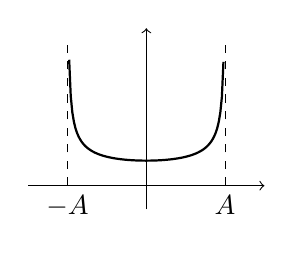
\begin{tikzpicture}[scale=1.0]
        % axis
        \draw[->] (-1.5,0) -- (1.5, 0);
        \draw[->] (0,-0.3) -- (0, 2);
    
        % % \node[below] at (3.1,0) {$r$};
    
        \draw[domain=-0.98:0.98
        ,thick,samples=100] plot (\x,{1/(pi*sqrt(1-\x*\x))});
    
        \draw[dashed] (-1, 0) -- (-1, 1.8);
        \draw[dashed] (1, 0) -- (1, 1.8);
        \node[below] at (-1,0) {$-A$};
        \node[below] at (1,0) {$A$};
    
    \end{tikzpicture}
    \caption{经典谐振子的概率密度}
\end{figure}
\suppInfo{经典谐振子的概率密度}{
从牛顿方程可以解得谐振子的轨迹
\begin{equation}
    x = A \sin (\omega t + \varphi),
\end{equation}
坐标方向的概率相当于 $\rho(x) = \frac{\dd t}{\dd x}$,反解出
\begin{equation}
    t = \frac{-\arcsin\frac{x}{A}-\varphi
   +\pi }{\omega }
\end{equation}
求导得到
\begin{eqnarray}
    \frac{\dd t}{\dd x} = -\frac{1}{\omega  \sqrt{A^2-x^2}},
\end{eqnarray}
归一化后即可得到密度分布。
}

\subsection{量子谐振子的概率密度}

经典图像中,在超出 $|A|$ 的区域中,概率是为 0 的,所以有了经典振幅的概念。

量子谐振子的波函数为
\begin{align}
    \psi_n(y) = A_n H_n(y) \exp^{-y^2/2}, \quad n=0,1,2,\cdots,
\end{align}
概率密度为模方,
\begin{align}
    |\psi_n(y)|^2 = |A_n|^2 \ee^{-y^2} |H_n (y)|^2 
    = \frac{a}{2^n n! \sqrt{\pi}} \ee^{-y^2} |H_n(y)|^2,
\end{align}

引入经典禁区 (classical restricted area) 的概念,谐振子的势能是 $V(x) = \frac 12 m\omega^2 x^2$,量子化的条件
\begin{align}
    \hbar\omega \left(n+\frac12\right) = \frac12 m\omega^2 \bar A_n^2,
\end{align}
其中 $\bar A_n$ 为量子振幅,那么
\begin{align}
    \bar A_n = \sqrt{\frac{2\hbar}{m\omega} \left(n+\frac12\right)} = \frac1a \sqrt{2n+1},
\end{align}
利用 $y=ax$,那么
\begin{align}
    \bar a_n = a \bar A_n = \sqrt{2n+1}
\end{align}
为无量纲振幅。

对于基态,
\begin{align}
    |\psi_0(y)|^2 = \frac{a}{\sqrt{\pi}} \ee^{-y^2},
\end{align}
依然是个高斯展宽,经典禁区的概率
\begin{align}
    Q_0 &= \int_{-\infty}^{-\bar A_n} |\psi_0(x)|^2 \dd x + \int_{\bar A_n}^{\infty} |\psi_0(x)|^2 \dd x \\
    &= 2 \int_{-\infty}^{-\bar A_n} |\psi_0(x)|^2 \dd x \\
    &= \frac{2}{\sqrt{\pi}} \int_{\bar a_0}^{\infty} \ee^{-y^2}\,\dd y \\
    &= \mathrm{erfc}(y),
\end{align}
% II $ x=\bar a_0 = 1$, 
同理计算出 $Q_0 = 0.157$, $Q_1 = 0.112$, $Q_2 = 0.095$, $\cdots$, $Q_{10} = 0.060$, $\cdots$。
\begin{lstlisting}
Clear["Global`*"]
\[Psi][n_, x_] := ((m \[Omega])/(\[Pi] \[HBar]))^(1/4) 1/Sqrt[2^n n!]
    HermiteH[n, 
    Sqrt[(m \[Omega])/\[HBar]] x] Exp[-1/2 (m \[Omega])/\[HBar] x^2];
n = 10;
Integrate[
    2 \[Psi][n, 
    x]^2, {x, -Infinity, -Sqrt[(2 \[HBar])/(m \[Omega]) (n + 1/2)]}, 
    Assumptions -> {m > 0, \[Omega] > 0, \[HBar] > 0}]
N[%]
>> (19634522823 Sqrt[21/\[Pi]])/(640 E^21) + Erfc[Sqrt[21]]
>> 0.0601438
\end{lstlisting}

当 $n$ 较大时,与量子情况较为接近。
\begin{lstlisting}
(* 画图,n 较大时的密度分布 *)
m = 1; \[Omega] = 1; \[HBar] = 1;
\[Psi][n_, x_] := ((m \[Omega])/(\[Pi] \[HBar]))^(1/4) 1/Sqrt[2^n n!]
    HermiteH[n, Sqrt[(m \[Omega])/\[HBar]] x] 
    Exp[-1/2 (m \[Omega])/\[HBar] x^2];
n = 10;
Plot[
    {\[Psi][n, x]^2, 
    (Pi Sqrt[(2 \[HBar])/(m \[Omega]) (n + 1/2) - x^2])^-1}, 
    {x, -6, 6}]
\end{lstlisting}


% \section{复习}
\courseTime{Oct 17, 2022 \\ 5th}
上周被关了多久(笑)?上周是第一次线上上课,讲课特别不舒服。

上周讲了量子谐振子。这个科学问题来自氢分子的势能面,不管是定性还是定量,都要跟分子间相互作用打交道,包括弱相互作用、强相关作用等等。

在解离势能面最低点是平衡构型,这点能量与解离能量的差是解离能 $D_{\mathrm e}$。氢分子的势能也可以用单侧无限深势阱描述,类似束缚态。由品优波函数的条件,得到束缚态的超越方程 $\cot z = - \sqrt{\left(\frac{z_i}z\right)^2 - 1}$,解之得离散化的能量 $\{z_i\}$。这个模型预测零点能,误差极大。所以我们知道,想要预测整体性质——零点能,需要在平衡位置接近真实势能,特别是平衡位置的曲率。

从平衡位置做泰勒展开,那么得到了抛物势 $V(x) = \frac12 m \omega x^2$,即谐振子模型。利用品优条件求解它,得到了量子化的解。最重要的品优条件是无穷远处不能发散,由此得到了 Hermite 方程、间隔的递推公式,其中的发散项让我们必须在某项截断它。最终解得零点能 $E_i = \hbar\omega\left(n + \frac12\right)$。相比于单侧无限深势阱,这个的势能形状更符合氢气的解离曲线。值得关注的是,能级间隔是相等的 $\Delta E = \hbar\omega$,当氢分子偏离平衡位置时,非谐振效应体现出来,只能描述低振动级别的振动态,这是谐振子模型无法描述的,而单侧无限深势阱区分了束缚态和解离态。

我们引入更符合真实的 Morse 势,其定义为
\begin{eqnarray}
    V(x) = D_{\mathrm e} \ee^{-a (r-r_\mathrm e)} ( \ee^{-a (r - r_\mathrm e)} - 2),
\end{eqnarray}
在平衡处 $r_\mathrm e$ 有最小值,在无穷远处为 0。Morse 势的薛定谔方程有解。
\begin{lstlisting}
(* 画出 Morse 势能的图 *)
Clear["Global`*"]
De = 1; \[Alpha] = 1; re = 1;
M[r_] := De (1 - Exp[-\[Alpha] (r - re)])^2
Plot[M[r], {r, 0, 5}]
\end{lstlisting}
\homework{\textbf{5.1} 比较谐振子与 Morse 势能函数,参考 JCP 1988, 88(7) 4535 ``The Morse oscillator in position space and phase space''}
越接近真实体系,薛定谔方程越难求解。从没有限制的自由粒子开始,到简单的势能(仅通过边界条件求解),到现在势能形状也接近真实物理。当势能复杂到无法解析求解时,便可以通过数值求解。
\homework{\textbf{5.1} (\emph{continued}) (选做)采用 Numerov 方法数值求解。见 Levin \emph{Quantum Chemistry} Sec 4.4 P70}

\chapter{粒子的转动与角动量}
为什么要学习转动,因为真实体系不止有平动,还有转动、振动等。

从基本公设出发,可以解薛定谔方程求出体系的波函数。对体系了解程度,在于波函数的精确程度,求解的困难程度在于势函数的复杂性。

前面解了那么多的体系,共同点是一维的。从一维拓展到二维,最简单的还是自由粒子,哈密顿算符
\begin{align}
    \hat H = -\frac{\hbar^2}{2m} \left(\pdv[2]{x} + \pdv[2]{y}\right),
\end{align}
那么薛定谔方程
\begin{align}
    \hat H \Psi(x,y) = E \Psi(x,y)
\end{align}
我们希望波函数可以分离变量,
\begin{align}
    \Psi(x,y) = X(x) Y(y), \label{eq:2dtrans_sepXY}
\end{align}
得到左右两边相互独立的式子,
\begin{align}
    \hat F(x) X(x) = \hat G(y) Y(y)
\end{align}
数学上可以证明上式等价于
\begin{align}
    &\hat F(x) X(x) = C, \\
    &\hat G(y) Y(y) = C. 
\end{align}

将 \eqref{eq:2dtrans_sepXY} 代回薛定谔方程,
\begin{align}
    -\frac{\hbar}{2m} \left(\pdv[2]x + \pdv[2]y\right) X(x) Y(y) &= E X(x) Y(y) \\
    -\frac{\hbar^2}{2m} Y(y) \pdv[2]x X(x) - \frac{\hbar^2}{2m} X(x) \pdv[2]y Y(y) &= E X(x) Y(y) \\
    -\underbrace{\frac{\hbar^2}{2m} \frac1{X(x)} \pdv[2]x X(x)}_{\text{只与 $x$ 有关}} - 
    \underbrace{\frac{\hbar^2}{2m} \frac1{Y(y)} \pdv[2]y Y(y)}_{\text{只与 $y$ 有关}} &= E,
\end{align}
物化上应该讲过这种变换,分离得到只与 $x$ 或 $y$ 有关的两项。

\section{环上运动的粒子}
\begin{figure}[tp]\centering
    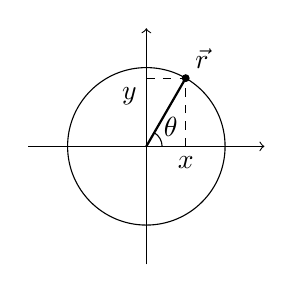
\begin{tikzpicture}[scale=1.0]
        % axis
        \draw[->] (-1.5,0) -- (1.5, 0);
        \draw[->] (0,-1.5) -- (0, 1.5);
        
        \draw (0,0) circle (1.0);
        \fill (0.5, 0.866) circle (0.05);
        \draw[dashed] (0.5, 0) -- (0.5, 0.866);
        \draw[dashed] (0, 0.866) -- (0.5, 0.866);
        \draw[thick] (0,0) -> (0.5, 0.866);
        \node[below] at (0.5, 0) {$x$};
        \node[below left] at (0.0, 0.866) {$y$};
        \node[above right] at (0.5, 0.866) {$\vec{r}$};
        \draw (0.2,0) arc (0:60:0.2);
        \node[above right] at (0.1,0) {$\theta$}; 
    
    \end{tikzpicture}
    \caption{环上的粒子}
\end{figure}
势函数
\begin{align}
    V(x,y) = \begin{cases}
        0, \quad & \sqrt{x^2 + y^2} = R,\\
        \infty, \quad &\sqrt{x^2 + y^2} \neq R, 
    \end{cases}
\end{align}
% 【讨论势能】
写出哈密顿量
\begin{align}
    \hat H = -\frac{\hbar^2}{2m} \left(\pdv[2]x + \pdv[2]y\right) + V(x,y)
\end{align}
此时无法分离变量 $\psi(x,y) \neq X(x) Y(y)$。如果将其变换到极坐标下,那么便可以分离变量,
\begin{align}
    \psi(r,\theta) = R(r) \Theta(\theta)
\end{align}
到底能否分离变量,求解完了才知道。

对波函数变换之后,还要把动能算符变换到极坐标下。这种变换相当于高中的难题,暴力求解比较麻烦,通常需要在求解开始时做非常巧妙的代换。尝试直接求解,首先,波函数的偏导不管在任何坐标下都是相等的,
\begin{align}
    \pdv[2]x \psi(x,y) = \pdv[2]{x} \psi(r,\theta),
\end{align}
用链式法则求解
\begin{align}
    &\pdv{\psi}{x} = \pdv{\psi}{r} \pdv{r}{x} + \pdv{\psi}{\theta} \pdv{\theta}{x},\\
    &\pdv{\psi}{y} = \pdv{\psi}{r} \pdv{r}{y} + \pdv{\psi}{\theta} \pdv{\theta}{y},
\end{align}
有几个显然的关系,
\begin{align}
    r^2 = x^2 + y^2, \quad \sin \theta = \frac xr,\quad \cos\theta = \frac yr,
\end{align}
径向对坐标的偏导,
\begin{align}
    \pdv{r}{x} = \pdv{x} \sqrt{x^2 + y^2} = \frac 12 \frac{2x}{\sqrt{x^2 + y^2}} = \frac xr = \cos\theta,
\end{align}
角度对坐标的偏导,利用 $\theta = \arccos \frac xr, x\in[0,\pi)$,
\begin{align}
    \pdv{\theta}{x} &= \pdv{x} \arccos \frac xr = -\frac1{\sqrt{1- \frac{x^2}{r^2}}} \left(\frac xr\right)^{\prime} \\
    &= -\frac ry \left(\frac 1r - \frac x{r^2} \frac xr\right) 
    = -\frac 1y \left(1 - \frac{x^2}{r^2}\right) \\
    &= -\frac{y}{r^2} = - \frac{\sin\theta} r, 
\end{align}
以上化简假设了 $\theta$ 在第一象限($x,y>0$),对于三四象限的角($y < 0$)需要加负号。
\begin{lstlisting}
(* 第一象限内的偏导 *)
D[ArcCos[x/Sqrt[x^2 + y^2]], x];
Simplify[%, Assumptions -> {x > 0, y > 0}]
>> -(y/(x^2 + y^2))
\end{lstlisting}

% 2022-10-17 08:54:22  Wenbin Fan @FDU
% 第二节课
% 下面得快一点了
那么对于波函数的导数
\begin{align}
    \pdv{\psi(x,y)}{x} = \cos\theta \pdv{\psi(r,\theta)}{r} - \frac{\sin\theta} r \pdv{\psi(r,\theta)}{\theta}, 
\end{align}
所以直接可给出
\begin{align}
    & \pdv{x} = \cos\theta \pdv{r} - \frac{\sin\theta}r \pdv{\theta},\\
    & \pdv{y} = \sin\theta \pdv{r} + \frac{\cos\theta}{r} \pdv{\theta},
\end{align}

再做二次偏导
\begin{align}
    \pdv[2]{\psi(x,y)}{x} = \pdv{x} \left(\cos\theta \frac{\psi}r - \frac{\sin\theta}r \pdv{\psi}{\theta}\right)
    \label{eq:polar_2nd_derv}
\end{align}
其中第一项
\begin{align}
    \pdv{x} \left(\cos\theta\pdv{\psi}{r}\right) 
    &= \pdv{\cos\theta}{x}\pdv{\psi}{r} + \cos\theta \pdv{x} \pdv{\psi}{r} \\
    &=\frac{\sin^2\theta}{r} \pdv{\psi}{r} + \cos\theta \left(\pdv[2]{\psi}{r} \pdv{r}{x} + \pdv[2]{\psi}{r}{\theta} \pdv{\theta}{x}\right) \\
    & = \frac{\sin^2\theta}{r} \pdv{\psi}{r} + \cos\theta \left( \cos\theta \pdv[2]{\psi}{r} - \frac{\sin\theta}{r} \pdv[2]{\psi}{r}{\theta}\right)
\end{align}
利用了
\begin{align}
    \pdv{x} \cos\theta = - \sin\theta \pdv{\theta}{x} = \frac{\sin^2\!\theta}{r},
\end{align}
第二项
\begin{align}
    \pdv{x} \left(\frac{\sin\theta}{r}\pdv{\psi}{x}\right) 
    &= - \frac{2\sin\theta \cos\theta}{r^2} \pdv{\psi}{\theta} + \frac{\sin\theta}r \left(\pdv[2]{\psi}{r}{\theta} \pdv{r}{x} + \pdv[2]{\psi}{\theta} \pdv{\theta}{x}\right)\\
    &=- \frac{2\sin\theta\cos\theta}{r^2} \pdv{\psi}{\theta} + \frac{\sin\theta \cos\theta}{r} \pdv[2]{\psi}{r}{\theta} - \frac{\sin^2\theta}{r^2} \pdv[2]{\psi}{\theta},
\end{align}
利用了
\begin{align}
    \pdv{x} \frac{\sin\theta}{r} = \pdv{x} \frac{y}{r^2} = \frac{-2y}{r^3} \pdv{r}{x} = -\frac{2\sin\theta\cos\theta}{r^2},
\end{align}
\begin{lstlisting}
(* 对 x 的二阶偏导,输出略 *)
D[\[Psi][Sqrt[x^2 + y^2], ArcCos[x/Sqrt[x^2 + y^2]]], {x, 2}];
Simplify[%, 
   Assumptions -> {x > 0, y > 0}] /. {y -> Sqrt[
    r^2 - r^2 Cos[\[Theta]]^2], x -> r Cos[\[Theta]]};
Simplify[%, Assumptions -> {r > 0, \[Theta] > 0, \[Theta] < Pi/2}]
\end{lstlisting}
于是
\begin{align}
    \pdv[2]{\psi(x,y)}{x}     
    &= \pdv{x} 
    \left(\cos\theta \pdv{\psi}{r} - \frac{\sin\theta}{r} \pdv{\psi}{\theta}\right) \\
    &= \cos^2\theta \pdv[2]{\psi}{r} - \frac{2\sin\theta\cos\theta}{r} \pdv[2]{\psi}{r}{\theta} + \frac{\sin^2\theta}{r^2} \pdv[2]{\psi}{\theta} \notag \\
    &\phantom{=} \quad + \frac{\sin^2\theta}{r} \pdv[2]{\psi}{r} + \frac{2\sin\theta\cos\theta}{r^2} \pdv{\psi}{\theta},
\end{align}
同理
\begin{align}
    \pdv[2]{\psi(x,y)}{y} &= \sin^2\!\theta \pdv[2]{\psi}{r} + \frac{2\sin\theta \cos\theta}{r} \pdv[2]{\psi}{r}{\theta} + \frac{\cos^2\theta}{r^2} \pdv[2]{\psi}{\theta} \notag\\
    &\phantom{=}\quad+ \frac{\cos^2\theta}{r} \pdv{\psi}{r} - \frac{2\sin\theta \cos\theta}{r^2} \pdv{\psi}{\theta}, 
\end{align}
于是 \eqref{eq:polar_2nd_derv} 为
\begin{align}
    \pdv[2]{\psi}{x} + \pdv[2]{\psi}{y} &= \pdv[2]{\psi}{r} + \frac1{r^2} \pdv[2]{\psi}{\theta} + \frac1r \pdv{\psi}{r} \\
    &=\pdv[2]{\psi}{r} + \frac1r \pdv{\psi}{r} + \frac1{r^2}\pdv[2]{\psi}{\theta}, 
\end{align}

最终哈密顿量写为
\begin{align}
    \hat H = - \frac{\hbar^2}{2m} \left(\pdv[2]{x} + \pdv[2]{y}\right) = -\frac{\hbar^2}{2m} \left(\pdv[2]{\psi}{r} + \frac1r \pdv{\psi}{r} + \frac1{r^2}\pdv[2]{\psi}{\theta}\right),
\end{align}
考虑本例中势能的特殊性,其径向部分为常数 $R$,因此哈密顿量仅与 $\theta$ 有关,
\begin{align}
    \hat H = - \frac{\hbar^2}{2mR^2} \pdv[2]{\theta} = -\frac{\hbar^2}{2I} \pdv[2]{\theta},
\end{align}
其中
\begin{eqnarray}
    I = m R^2
\end{eqnarray}
称之为\boldtext{转动惯量} momentum of inertia。%注意到 $\omega = \theta / t$,

薛定谔方程为
\begin{align}
    \hat H \varphi(\theta) &= E\varphi(\theta)\\
    - \frac{\hbar^2}{2I} \pdv[2]{\varphi}{\theta} &= E\varphi
\end{align}
整理得到
\begin{align}
    \pdv[2]{\varphi(\theta)}{\theta} + M^2 \varphi(\theta) = 0, \quad M^2 = \frac{2IE}{\hbar^2},
\end{align}
这是个二阶微分方程,设 $\varphi(\theta) = \ee^{s\theta}$,有
\begin{align}
    s^2 \ee^{s\theta} + M^2 \ee^{s\theta} = 0
\end{align}
得到
\begin{align}
    s^2 = - M^2 \Rightarrow s = \pm \ii M,
\end{align}
可得方程通解
\begin{align}
    \varphi(\theta) = A \ee^{\ii M\theta} + B \ee^{-\ii M \theta}
\end{align}
共有三个待求变量 $\{A, B, M\}$。

给出通解之后,利用边界条件得到量子化结果。在解无限深势阱的时候,利用了波函数连续、导数连续的条件。我们这里的二位极坐标体系,边界就是粒子转过 $2\pi$ 后又回来,所以有周期性边条件,
\begin{align}
    \varphi(\theta) = \varphi(\theta + 2\pi),
\end{align}
解得
\begin{align}
    \ee^{\ii M\, 2\pi} = 1 \Rightarrow M = 0, \pm 1, \pm 2, \cdots,
\end{align}
这里的 $M$ 称之为磁量子数 magnetic quantum number,从而可以解出能量
\begin{align}
    M^2 = \frac{2IE}{\hbar^2} \Rightarrow E = \frac{M^2\hbar^2} {2I} = \frac{M^2h^2} {8\pi^2 L},
\end{align}
知道了分子的转动惯量,就可以求出转动的精确谱、能量间隔。


讲到了转动,就必须要讲到角动量。角动量算符在经典力学中的定义为
\begin{align}
    \bm L = \bm r \times \bm p = \bm r \times m\bm v, 
\end{align}
对应的是右手定则。
分量形式
\begin{align}
    &L_x = y p_z - zp_y, \\
    &L_y = z p_x - x p_z, \\
    &L_z = x p_y - y p_x, 
\end{align}
微观体系中角动量是什么样的?

角动量的量子化 quantization,
\begin{align}
    \hat L_z = x \hat p_y - y \hat p_x = - \ii \hbar \left(x \pdv{y} - y \pdv{x}\right),
\end{align}
可以通过极坐标的变化求解出极坐标下的表达式,
\begin{align}
    \hat L_z = -\ii \hbar \pdv{\theta},
\end{align}
作为作业。
\homework{\textbf{5.2}  推导极坐标下的 $z$ 轴角动量算符 $\hat L_z$ 表达式。}
有个问题,我们说是量子化,其实直接用了动量算符的定义,但这是演绎,不是推导。如果在经典情况,$x$ 的位置无所谓,放在算符前后均可,以便跟量子情况相对于,实际上量子化不是直接加个 $\hat\cdot$ 得到的,角动量的量子化过程不具有普适性。

已经求出了环上粒子的通解,将
角动量算符作用到通解波函数上,
\begin{align}
    \hat L_z \varphi(\theta) \overset{?}{=} C\varphi(\theta),
\end{align}
会得到常数 $C$ 吗?不一定对吧,作用上去之后会有两个相反的系数 $\ii m$。这就很像动量算符和动能算符的关系,我们知道动量算符、动能算符是互易的,原则上可以共享同一个本征函数。
% \homework{\textbf{5.2} (\emph{continued}) 证明}

环上粒子的哈密顿量 $\hat H$ 和角动量 $\hat L_z$ 显然是对易的,所以它们可以共享相同的本征函数。通过构造本征函数,能求出通解,因为 $m$ 是任意的。并不要求角动量的本征函数是 $z$ 方向的。

量子力学基本假设第四条告诉我们,线性厄米算符给出来的本征函数是完备集,意思是任何函数都可以用这个完备集展开。二者共享本征函数的意思是,那么用这个共享的本征函数可以描述任何状态,无需只用一个或另一个,那么通解中的 $A$ 和 $B$ 可以去掉其中一个。剩下的一个代表它既是哈密顿量的本征函数,也是 $\hat L_z$ 的本征函数。

我们在实际的体系中,为什么要做这个事儿?正常来说,我们解薛定谔方程,通常只要基态能量,并不关心波函数是否是 $\hat L_z$ 的本征函数。在真实观测中,观测到的不仅是基态,还有各种的激发态。比如磁场下的分子,光谱中能看到各种磁量子数导致的细分。
% 【一大段讲述】
% 实际体系光谱,还有磁量子数。
% 状态波函数不仅是【】还是【】的本征函数,所以这个态是为了解磁量子数时光谱的细分【】。

在解氢原子体系时,能量只与 $n$ 有关。通过连带勒让德方程,还有 $m_l$ 等量子数。哈密顿算符是不区分 2p$_{-1}$、2p$_1$ 等,从实验中是可以同时准确观测到分量的。为什么能准确测量能量,同时在光谱中看到精确的磁量子数?因为哈密顿算符 $\hat H$ 和角动量 $\hat L$ 是对易的。动能和位置算符是不对易的,所以无法同时准确测量。

% 2022-10-17 13:24:54  Wenbin Fan @FDU
% 下午
\courseTime{下午}
简单回顾下早上的内容。想要了解任何感兴趣的体系,都要解薛定谔方程。目前的波函数都是不含时的,即定态方程。今天求解的势能函数是二维的,这是与之前最大的不同。通常二维势能难以在 Cartesian 空间求解,由合适的坐标变换可以简化求解过程。最契合环势能的坐标是极坐标,因此很自然地分离变量。

将环形势能变换到极坐标下,此时哈密顿量仅与 $\theta$ 有关,引入周期性边条件,得到磁量子数。随后演绎了角动量 $\hat l_z$ 的算符表示。

环运动的通解是两个本征函数的线性组合,包含了顺时针和逆时针旋转的组合。哈密顿算符和 $\hat l_z$ 是队医的,可以构造同时属于二者的本征函数完备集,所以可以把 $\varphi(\theta)$ 写成 $A \ee^{\ii m \varphi}$ 的形式。

接上午的求解。由归一化确定 $A$,
\begin{align}
    \int_0^{2\pi} \varphi^*(\theta) \varphi(\theta) \dd\theta = A^2 \int_{0}^{2\pi} \dd\theta = 2\pi A^2 = 1,
\end{align}
解之得
\begin{align}
    \varphi(\theta) = \frac{1}{\sqrt{2\pi}} \ee^{\ii m \theta}, \quad \rho(\theta) = |\varphi(\theta)|^2 = \frac1{2\pi},
\end{align}
因此波函数没有节点,任何地方的取值都是一样。我们现在求解的模型,都是希望贴近化学真实体系,与这个模型最相近的是苯环。
\homework{\textbf{5.2}  对于一维环形势箱,其能级为 
\begin{align}
    E_n = \frac{n^2 h^2}{8\pi^2 m R^2}, \quad n = 0, 1, 2, \cdots,
\end{align}
苯环的 $\pi$ 电子可近似看成是电子限制在一个环上的运动,$\pi$ 电子的半径是 \SI{1.4}{\angstrom},请以一维环形势箱的模型计算其最低激发能。

(以下选做)激发能的实验值是 \SI{2600}{\angstrom},讨论误差可能的来源。
}
随意讨论,真实的苯和离域电子的区别是什么。下周习题课,再下次求解熟悉的氢原子,我们现在从二维拓展到三维,为求解氢原子做准备。

\section{柱面上的粒子}
先讲一个简单的三维体系,(同学:球)真会找,找了个最难的。最简单的是自由粒子,三维自由粒子的算符,
\begin{align}
    \hat H = -\frac{\hbar^2}{2m} \left(\pdv[2]{x} + \pdv[2]{y} + \pdv[2]{z}\right), \quad \hat H \psi(x,y,z) = E \psi (x,y,z),
\end{align}
通过分离变量,可以解耦,求出来各个分量的波函数。

其次是无限深势阱的拓展,三维势能箱。比球简单一些的(安静),是圆柱啊!圆柱可以分离变量。接近真实的碳纳米管,这里以铜丝为例。
\homework{\textbf{5.3}  一圆柱体,长为 $l$、半径为 $R$,求解该圆柱体体系的能级,这里的势函数定义为
\begin{align}
    V(x,y,z) = \begin{cases}
        0, \quad &(x,y,z) \in \Omega,\\
        +\infty, \quad &(x,y,z) \notin \Omega,
    \end{cases}
\end{align}
其中
\begin{align}
    \Omega = \left\{(x,y,z) \, |\,  x^2+y^2 \leqslant R^2, 0\leqslant z\leqslant l\right\}. 
\end{align}
可参考徐昕老师 2000 年的文章 Jian-Lin Yao, Xin Xu, De-Yin Wu, et al, \emph{Chem. Commum.} 2000, 1627。
}
这些东西已经超越了课堂内容,但也确实是关于课堂内容触手可及的拓展。如果你会算这些习题,其实你已经可以做一些科研工作了。

现在计算机发达,很多人已经习惯了用 Gaussian 软件,用各种基函数展开波函数。
% 【】有助于掌握背后的物理。
化学从简单模型演变到复杂,越来越难算,主要源自于实验的精度越来越高。早期的实验,可控性很差,无法控制合成多孔材料、超分子等,无法控制形貌,只能通过宏观的温度等辅助合成。当近代实验操控能力增强,比如精准化学可以 100\% 操控反应物和产物,人们能制造出更精确的催化剂。这时计算化学便可以辅助实验,得到活性最高的形貌。
% 精确操控形状,什么形状有用?
% 【】【】【】【】【】

再复杂一点的,是球面上运动的粒子。

\section{球面上运动的粒子}
哈密顿量写出来
\begin{align}
    \hat H = -\frac{\hbar^2}{2m} \left(\pdv[2]x + \pdv[2]y + \pdv[2]z\right) + V(x,y,z),
\end{align}
其中势能
\begin{align}
    V(x,y,z) = \begin{cases}
        0, \quad &\sqrt{x^2+y^2+z^2} = r = R, \\
        \infty, \quad &\text{其它},
    \end{cases}
\end{align}
画出势能,坐标轴的定义是右手定则(四指从 $x$ 转向 $y$,大拇指指向 $z$),注意这里的 $\theta$ 是 $\bm r$ 与 $z$ 轴的夹角。
\begin{figure}
    \centering
    \includegraphics[width=3cm]{fig/angular_momentum.png}
    \caption{角动量方向}
    \label{fig:ang_direction}
\end{figure}

定义好坐标轴后,写出坐标映射
\begin{align}
    & x= r\,\sin\theta \, \cos\varphi, \\
    & y = r\,\sin\theta \, \sin\varphi, \\
    & z = r\,\cos\theta,
\end{align}
体积元变化
\begin{align}
    \Delta V = \Delta x \,\Delta y\, \Delta z,
\end{align}
\begin{figure}[tbp]
    \centering
    \includegraphics[width=4cm]{fig/3d_int_element.png}
    \caption{求坐标中的积分微元}
    % ref: https://blog.csdn.net/TanWaiwai_yy/article/details/104710427
\end{figure}
根据推导,有
\begin{align}
    \Delta V & =\dd s \, \dd r \\
    & = r \, \dd\theta \, r\sin\theta \, \dd\varphi \dd r \\
    & = r^2 \sin\theta \dd\theta \dd\varphi \dd r,
\end{align}
暴力推导的话,今天就别下课了。这里利用高级的数学方法,即利用 Jacob 矩阵来变换坐标系,
\begin{align}
    J = 
    \begin{pmatrix}
    \pdv{x}{r} & \pdv{x}{\theta} & \pdv{x}{\varphi} \\
    \pdv{y}{r} & \pdv{y}{\theta} & \pdv{y}{\varphi} \\
    \pdv{z}{r} & \pdv{z}{\theta} & \pdv{z}{\varphi}
    \end{pmatrix}, \quad 
    \begin{pmatrix}
        \pdv{r} \\ \pdv{\theta} \\ \pdv{\varphi}
    \end{pmatrix}
    = J 
    \begin{pmatrix}
        \pdv{x} \\ \pdv{y} \\ \pdv{z}
    \end{pmatrix},
\end{align}
直接得到结果,动能算符在极坐标下的表述,
\begin{align}
    \hat T = - \frac{\hbar^2}{2m} \left(
        \pdv[2]r + \frac2r \pdv{r} + \frac1{r^2} \hat \Lambda^2
    \right),
\end{align}
其中
\begin{align}
    \hat \Lambda ^2 &= \frac1{\sin^2\theta} \pdv[2]{\varphi} + \frac1{\sin\theta} \pdv{\theta} \left(\sin\theta \pdv{\theta}\right) \\
    & = \frac1{\sin^2\theta} \pdv[2]{\varphi} + \cot\theta \pdv{\theta} + \pdv[2]{\theta},
\end{align}
这个算符 $\hat \Lambda$ 包含了动能中所有角度部分的能量,即角动量相关的能量,它一定与角动量相关。接下来很自然地考虑,三维的角动量如何考虑?

我们已经给出了二维的角动量,角动量的方向向外,沿着第三个坐标轴 $z$。角动量算符
\begin{align}
    \bm L = \bm r \times \bm p = \bm r \times m \bm v,
\end{align}
三个分量为
\begin{align}
    &\hat L_x = -\ii\hbar \left(y \pdv{z} - z \pdv{y}\right), \\
    &\hat L_y = -\ii\hbar \left(z \pdv{y} - y \pdv{z}\right), \\
    &\hat L_z = -\ii\hbar \left(x \pdv{y} - y \pdv{x}\right),
\end{align}
% 【还有两个式子没列上】
回顾两个例子中的解,
\begin{alignat}{2}
    &\text{二维极坐标} \quad &&\hat L_z = -\ii\hbar \pdv{\theta}, \\
    &\text{三维极坐标} \quad && \hat L_z = -\ii\hbar \pdv{\varphi},
\end{alignat}
% 【这里角动量分量好像不太对耶】
\homework{\textbf{5.4} 证明 
\begin{align}
    \hat L_x = -\ii\hbar \left(
        \sin\varphi \pdv{\theta} + \cot\theta \cos\varphi \pdv{\varphi}
    \right), \\
    \hat L_y = -\ii\hbar \left(
        \cos\varphi \pdv{\theta} - \cot\theta \sin\varphi \pdv{\varphi}
    \right),
\end{align}
并且利用
\begin{align}
    \hat L = \hat L_x \bm i + \hat L_y \bm j + \hat L_z \bm k
\end{align}
推导
\begin{align}
    \hat L^2 &= \hat L_x^2 + \hat L_y^2 + \hat L_z^2 \\&= -\hbar^2 \left(
        \frac1{\sin^2\theta} \pdv[2]{\varphi} + \cot\theta \pdv{\theta} + \pdv[2]{\theta}
    \right) \\
    &= -\hbar^2 \Lambda ^2,
\end{align}
}

% 【推导 theta varphi 相关的式子】
% 【必须求解耦合的方程了】
% 当前体系的哈密顿量,
% \begin{align}
%     \hat H = -\frac{\hbar^2}{2mR^2} \hat\Lambda^2 = \frac1{2mR^2} \hat L^2 = - \frac1{2I},
% \end{align}
薛定谔方程
\begin{align}
    -\frac{\hbar^2}{2mR^2} \hat \Lambda^2 Y(\theta,\varphi) = E Y(\theta, \varphi), 
\end{align}
% 2022-10-17 14:24:07  Wenbin Fan @FDU
% 最后一节啦!
径向部分的偏导全部为 0,那么能否分离变量?
\begin{align}
    Y(\theta,\varphi) \overset{?}{=} \Theta(\theta) \Phi(\varphi),
\end{align}
尝试分离后代回,
\begin{align}
    \hat \Lambda^2  \Theta(\theta) \Phi(\varphi) + M^2  \Theta(\theta) \Phi(\varphi) = 0,
\end{align}
把 $\hat \Lambda^2$ 的定义代入,
\begin{align}
    \left(\frac1{\sin^2\theta} \pdv[2]{\varphi} + \cot\theta \pdv{\theta} + \pdv[2]{\theta}\right) \Theta(\theta) \Phi(\varphi) + M^2  \Theta(\theta) \Phi(\varphi) = 0, \notag\\
    \frac{\Theta(\theta)}{\sin^2\theta} \pdv[2]{\varphi} \Psi(\varphi) + \cot\theta \Psi(\varphi) \pdv{\theta} \Theta(\theta) + \Psi(\varphi) \pdv[2]{\theta} \Theta(\theta) + M^2 \Theta(\theta) \Psi(\varphi) = 0,
\end{align}
两边同时除以 $\Theta(\theta) \Phi(\varphi)$,
\begin{align}
    \frac{1}{\sin^2\theta \Psi(\varphi)} \pdv[2]{\varphi} \Psi(\varphi) + \frac{\cot\theta}{\Theta(\theta)} \pdv{\theta} \Theta(\theta) + \frac1{\Theta(\theta)} \pdv[2]{\theta} \Theta(\theta) + M^2 &= 0 \notag\\
    \underbrace{\frac{1}{\Psi(\varphi)} \pdv[2]{\varphi} \Psi(\varphi)}_{\varphi} 
    + 
    \underbrace{\frac{\sin\theta\,\cos\theta}{\Theta(\theta)} \pdv{\theta} \Theta(\theta) + \frac {\sin^2\theta}{\Theta(\theta)} \pdv[2]{\theta} \Theta(\theta) + M^2 \sin^2\theta}_{\theta}
    &= 0,
\end{align}
第一项只跟 $\varphi$ 有关,后面三项只跟 $\theta$ 有关,所以可以分开,分别移动到等号两端
\begin{align}
    \frac{1}{\Psi(\varphi)} \pdv[2]{\varphi} \Psi(\varphi) = - \left[
        \frac{\sin\theta\,\cos\theta}{\Theta(\theta)} \pdv{\theta} \Theta(\theta) + \frac {\sin^2\theta}{\Theta(\theta)} \pdv[2]{\theta} \Theta(\theta) + M^2 \sin^2\theta
    \right]
    \label{eq:sphere_surface_sep_done}
\end{align}
令左侧等于常数 $N$
\begin{align}
    \frac{1}{\Psi(\varphi)} \pdv[2]{\varphi} \Psi(\varphi) = N \Rightarrow  \pdv[2]{\varphi} \Psi(\varphi) = N \Psi(\varphi), 
\end{align}
取 $\Psi(\varphi) = \ee^{s\varphi}$,当 $N>0$ 时,$s = \pm\sqrt N$,$\Psi(\varphi) = \ee^{\pm \sqrt N \varphi}$ 发散、非品优,舍弃。%【】【】【N<0】
当 $N<0$ 时,$s = \pm\ii\sqrt{-N}$,$\Psi(\varphi) = \ee^{\pm\ii\sqrt N}$。

设 $N = - m_l^2$,得到
\begin{align}
    \Psi(\varphi) = A \ee^{\ii m_l \varphi} + B \ee^{-\ii m_l \varphi},
\end{align}

% 【共同本征函数】
因为
$\hat L^2$ 与 $\hat L_z$ 的共同本征函数解,
\begin{align}
    \Psi(\varphi) = A \ee^{\ii m_l \varphi} = \frac1{\sqrt{2\pi}} \ee^{\ii m_l \varphi}, \quad m_l = 0, \pm1, \pm2, \cdots,
\end{align}
因为有共同的本征值,那么 \eqref{eq:sphere_surface_sep_done} 右侧 $\Theta$ 相关的项等于 $-m_l^2$,
\begin{align}
    - \left[
        \frac{\sin\theta\,\cos\theta}{\Theta(\theta)} \pdv{\theta} \Theta(\theta) + \frac {\sin^2\theta}{\Theta(\theta)} \pdv[2]{\theta} \Theta(\theta) + M^2 \sin^2\theta
    \right] = -m_l^2,
\end{align}
整理得
\begin{align}
    \sin\theta\cos\theta \pdv{\theta} \Theta(\theta) + \sin^2\theta \Theta(\theta) = (m_l^2 - M^2 \sin^2\theta) \Theta(\theta),
\end{align}
在以前求解的体系中,能量是完全量子化的,但是这里的 $\theta,\varphi$ 完全不是,因为二者的量子数相互有关系,关于 $\varphi$ 的量子数要代入到 $\theta$ 的求解中。

该方程的解称作\boldtext{连带勒让德多项式}。目前还是太复杂了些,做一些变量代换。首先三角函数看起来就很麻烦,替换掉,设 $x = \cos\theta$,则 $\Theta(\theta) = y(x)$,求这个代换的偏导数,
\begin{align}
    &\pdv{\theta}\Theta(\theta) = \pdv{y(x)}{x} \pdv{x}{\theta} = \pdv{y(x)}{x}(-\sin\theta),\\
    &\pdv[2]{\theta} \Theta(\theta ) = 
    -\cos \pdv{y(x)}{x} - \sin\theta \pdv[2]{y(x)}{x} \pdv{x}{\theta} \\
    &\phantom{\pdv[2]{\theta} \Theta(\theta )} = 
    -\cos \pdv{y(x)}{x} + \sin^2\theta \pdv[2]{y(x)}{x}, 
\end{align}
代换完了是
\begin{multline}
    - x(1-x^2) \pdv[2]{y(x)}{x} + (1-x^2) \left[
        -x \pdv{y(x)}{x} + (1-x^2) \pdv[2]{y(x)}{x}
    \right] \\= \left[m_l^2 - M^2(1-x^2)\right] y(x),
\end{multline}
观察到其中每一项都含有 $(1-x^2)$,两边同时除以它。按照导数的次数排列,有
\begin{align}
    (1-x^2) y''(x) - 2x\, y'(x) + \left(M^2 - \frac{ml^2}{1-x^2}\right) y(x) = 0.
    \label{eq:legendre_ordered} % 按导数次序排列的
\end{align}

现在还不能求解它,因为当 $x = \cos\theta = \pm1$ 时有奇点,必须先消除奇点。

\boldtext{(1) 消除奇点},当 $x = \pm 1$ 时,
\begin{align}
    y(x) = (1 - x^2)^n H(x),
\end{align}
书上会告诉你当 $n = \frac{|m_l|}2$ 时可以消除,那么为什么呢?我们从头开始推导这个结果,即直接把 $n$ 代回原式。求出偏导方便一些,
\begin{align}
    &\pdv{y(x)}{x} = -2n x (1-x^n)^{n-1} H_n(x) + (1-x^2)^n H'(x),
\end{align}
二阶偏导稍麻烦
\begin{align}
    \pdv[2]{y(x)}{x} &= -2n x \left[
        (1-x^2)^{n-1} - 2(n-1)x^2(1-x^2)^{n-2}
    \right]H(x)  \notag\\
    &\quad\quad
    - 2n x(1-x^2)^{n-1} H'(x) 
    - 2n x(1-x^2)^{n-1} H'(x) \notag\\
    &\quad\quad + (1-x^2)^n H''(x) \\
    & = \left[
        -2n (1-x^2)^{n-1} + 4n (n-1) x^2 (1-x^2)^{n-2}
    \right] H(x) \notag\\
    &\quad\quad - 4nx(1-x^2)^{n-1} H'(x) + 
    (1-x^2)^n H''(x)
\end{align}
这时候再代回原式 \eqref{eq:legendre_ordered}
\begin{multline}
    \left[
        -2n (1-x^2)^n + 4n(n-1) x^2 (1-x^2)^{n-1}
    \right] H(x) \\
    - 4nx(1-x^2)^n H'(x) + (1-x^2)^{n+1} H''(x) \\
    + 4nx^2 (1-x^2)^{n-1} H(x) 
    - 2x (1-x^2)^n H'(x) \\
    +\left[
        M^2 (1-x^2)^n - m_l^2 (1-x^2) ^{n-1}
    \right] H(x) = 0,
\end{multline}
合并同类项,
\begin{multline}
    (1-x^2)^{n+1} H''(x) - 2x(2n+1) (1-x^2)^n H'(x) 
    \\+ 
    \left[
        -2n (1-x^2)^n + 4n^2 x^2 (1-x^2)^{n-1} - m_l^2 (1-x^2)^{n-1} + M^2 (1-x^2)^n
    \right] H(x) \\= 0
\end{multline}
再化简,
\begin{align}
    (1-x^2) H''(x) - 2x(2n+1) H'(x) + \left[
        -2n + \frac{4n^2x^2 - m_l^2}{1-x^2} + M^2
    \right] H(x) = 0
\end{align}
也就是当 $4n^2 = m_l^2$ 时,有
\begin{align}
    \frac{m_l^2 (x^2 - 1)}{1 - x^2} = - m_l^2,
\end{align}
令 $n = \frac{|m_l|}2$,即
\begin{align}
    y(x) = (1 - x^2)^{|m_l|/2} H(x),
\end{align}
有
\begin{align}
    (1-x^2) H''(x) - 2\left(|m_l| + 1\right)x \, H'(x) + \left(m^2 - m_l^2 - |m_l|\right) H(x) = 0. 
\end{align}

整个解法从头到尾写下来很累的,但是每一步都有逻辑。量子的教科书上都是这个结论,读者难以知道整个过程。

在学习特殊函数或者数学物理方程时,最有创造性的一点是一开始选什么样的初猜,即选择什么样的通解。球面上的粒子也是一样,从尝试分离变量开始,再到消奇点,很幸运有连带勒让德函数这个解。

% 2022-10-17 15:08:33  Wenbin Fan @FDU
% 快下课了 XD
% 这段求解过程好乏味……
下节课继续讲幂级数求解法。












% 
\section{复习}
% 2022-10-24 07:59:36  Wenbin Fan @FDU
是人变少了吗,还是坐后面去了(笑)。

我们今天有节习题课,下周讲氢原子,慢慢接近于真实体系了,后面会安排上机,把我们的超算给同学们用。

今天要把上次课讲完,同时补充一些前面的内容。下午两节课习题课,助教来上。

上周课我们讲了转动角动量。

二维体系的时候,粒子在环形圆上运动,相当于势函数的边界条件跟 $r$ 能更好地分离变量,所以要做坐标变换,最关键的是动能部分的坐标变换。通过变换动能,得到了分离变量的哈密顿量。势函数是 delta 函数,因此哈密顿量跟自由粒子是一样的。

哈密顿量变换后,因为径向不变,其中对径向的偏导为 0,所以哈密顿量之跟角度有关。转动惯量定义为 $I = mr^2$。由周期性边界条件,得到了磁量子数。

随后定义了角动量,特别是 $z$ 轴的角动量。
由于 $l_z$ 互易,可以构造共同的本征函数完备集,
方向性可以体现在 $m$ 的正负上。一维拓展到三维。

对于球面上的粒子,与圆环上的粒子类似,势能只与 $r$ 有关,一样要做坐标变换。动能算符,其中的转动部分含有角度分量。二维中,$xOy$ 平面的角度是 $\theta$,三维中,角动量与 $z$ 轴的夹角是 $\theta$。

% $\hat L^2$ 的
第一次涉及到两个变量耦合的求解,成功地分离变量。

我们对勒让德方程做变换,是为了利用数学物理方程中的结论,更方便地求解。勒让德方程已经被研究得非常透彻。我们不是数学系、物理系,但鼓励学习数学物理方程、泛函分析等。
比如,导出薛定谔方程,需要有强大的数学直觉,我们现在学习也是为了以后寻找物理规律。

上节课讲到了\boldtext{幂级数展开},继续讲。勒让德方程里有一阶、二阶偏导,
\begin{align}
    H(x) = \sum_{j=0}^{\infty} a_j x^j, \quad H'(x) = \sum_{j=1}^{\infty} j a_j x^{j-1}, \quad H''(x) = \sum_{j=2}^{\infty} j(j-1) a_j x^{j-2},
\end{align}
得到了等间隔的递推公式
\begin{align}
    \sum_{j=1}^\infty
    \left\{
        (j+2)(j+1) a_{j+2} + \left[
            (j+ |m_l| +1) - M^2
        \right]a_j
    \right\} x^j = 0,
    % 2022-10-24 08:20:05  Wenbin Fan @FDU
\end{align}
若 $H(x)$ 是无穷级数,则 $H(x)$ 不是品优波函数。
所以,如果 $a_j$ 在 $k$ 截断,意味着这一项为 0,
\begin{align}
    a_{j+2} = \frac{(j+|m_l|)(j+|m_l|+1) - M^2}{(j+2)(j+1)} a_j,
\end{align}
参考 H. Eyring, J. Walter, Quantum Chemistry, \S 4. 

这里省略一些通用的推导。若 $H(x)$ 是无穷级数,则 $H(x)$ 不是品优波函数,当 $a_j$ 在 $k$ 截断,
\begin{align}
    (k+|m_l|)(k+|m_l|+1) - M^2 = 0, 
\end{align}
令 $l \equiv k + |m_l|$,则
\begin{align}
    M^2 = l(l+1),
\end{align}
其中
\begin{align}
    |m_l| = 0,1,2,\cdots, \quad l = 0,1,2,\cdots,
\end{align}
显然可知 $|m_l|_{\mathrm{max}} = l$。

% 2022-10-24 08:24:28  Wenbin Fan @FDU
再回到能量的量子化,体系的能量
\begin{align}
    - \frac{\hbar^2}{2m R^2} \hat\Lambda ^2 Y(\theta,\varphi) = E Y(\theta, \varphi), 
    \label{eq:LambdaYEY}
\end{align}
分离变量得到
\begin{align}
    \hat \Lambda^2 \Theta(\theta) \Phi(\varphi) + M^2 \Theta(\theta) \Phi(\varphi)  = 0,
\end{align}
其中
\begin{align}
    M = E \frac{2mR^2}{\hbar^2} = \frac{2IE}{\hbar^2},
\end{align}
得到了能量的量子化
\begin{align}
    E = \frac{\hbar^2}{2I} \, l (l+1), \quad l = 0,1,2,\cdots,
\end{align}
与此同时,如果找到二者共同的本征函数,一定会有本征角量子数,并且角量子数 $m_l = 0, \pm1, \pm2, \cdots, \pm l$。

因为哈密顿算符 $\hat H$ 和 $l_z$ 是对易的。如果取二者共同的本征函数,
两个算符作用上去,
就会有两个量子数 $m_l$ 和 $l$,这也就是为什么把 \eqref{eq:LambdaYEY} 写成
\begin{align}
    - \frac{\hbar^2}{2I} \hat\Lambda^2 Y_{l,m_l}(\theta, \varphi) = \frac{\hbar^2}{2I} l(l+1) Y_{l,m_l}(\theta, \varphi). 
\end{align}
我们知道 $\hat \Lambda$ 和 $\hat L$ 是等价的,$\hat L^2 = -\hbar^2\hat L^2$,那么代入这个等式,有
\begin{align}
    \frac{1}{2I} \hat L^2 Y_{l,m_l}(\theta, \varphi) &= \frac{\hbar^2}{2I} l(l+1) Y_{l,m_l}(\theta, \varphi) \\
    \hat L^2 Y_{l,m_l}(\theta, \varphi) &= \hbar l (l+1) Y_{l,m_l}(\theta, \varphi)\label{eq:6_l_squared}
\end{align}
很自然地给出了角动量算符在三维体系中的本征函数。

后面求氢原子体系,当然要做一些额外的坐标变换,其势能函数只与径向有关(库伦算符),角度部分是球谐形式,所以我们求解的也是氢原子的角度部分。

\eqref{eq:6_l_squared} 中也能推导出 $z$ 方向的本征值,
\begin{align}
    \hat L_z = -\ii\hbar \pdv{\varphi} \Rightarrow \hat l_z Y_{l,m_l}(\theta, \varphi) = m_l Y_{l,m_l}(\theta, \varphi), 
\end{align}
\begin{align}
    |m_l|_{\mathrm{max}} = l, \quad \langle \hat l_z \rangle ^2 |_{\mathrm{max}} = l^2, 
    \quad \langle \hat L^2 \rangle = l(l+1),
\end{align}
$z$ 方向一定有不确定性,类似于零点能。
% 【】一定会留下一份。
% 讲错了
% 2022-10-24 08:35:49  Wenbin Fan @FDU
也可以理解成「测不准原理」。
\begin{figure}
    \centering
    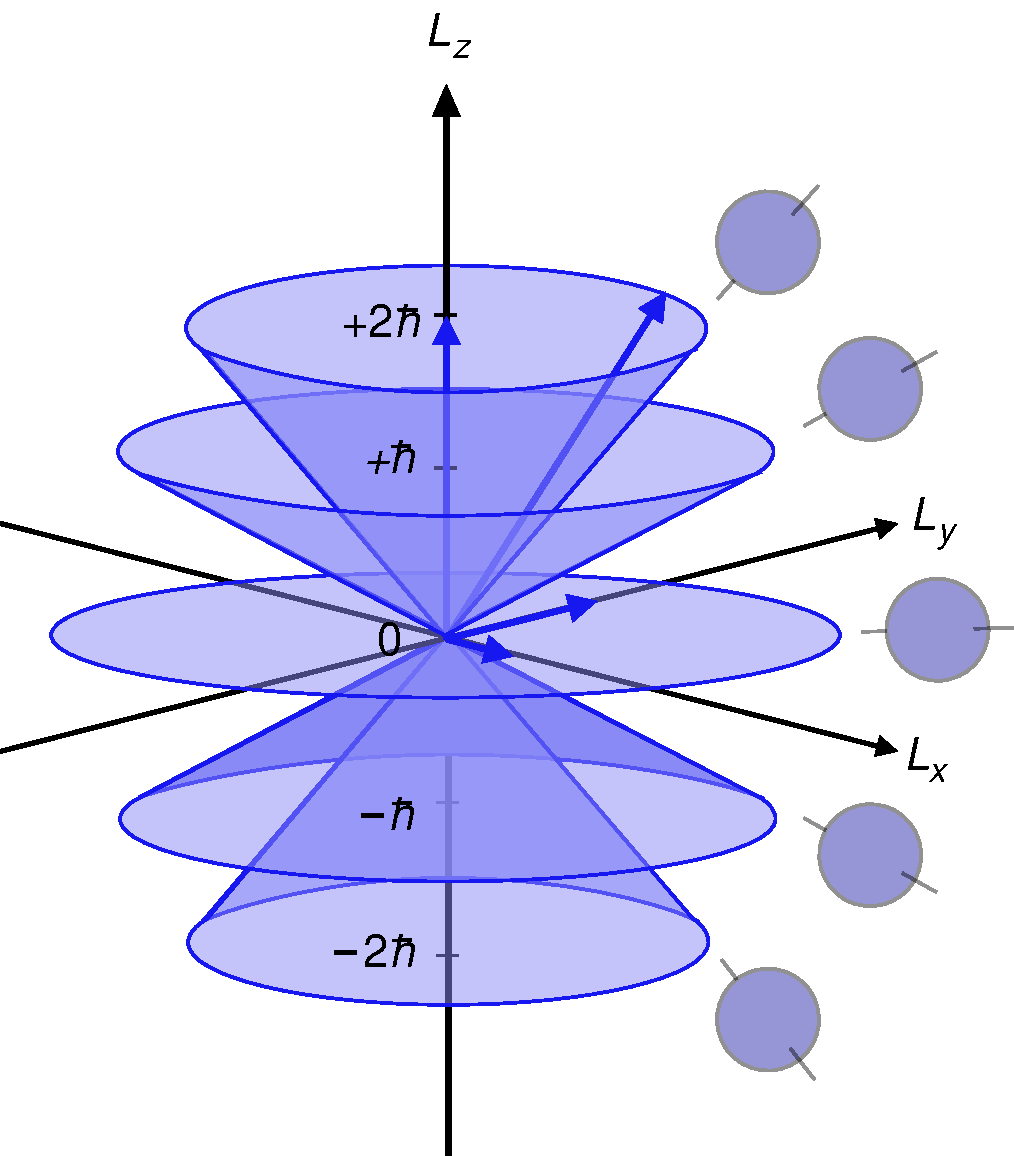
\includegraphics[height=3cm]{fig/angular_momentum_Wikipedia.pdf}
    \caption{角动量量子化}
\end{figure}

\homework{
    \textbf{6.1}  对于一个电子 $m_{\mathrm e} = \SI{9.11E-31}{\kilo\gram}$,以及一个陀螺 $m = \SI{0.02}{\kilo\gram}$,如果转动半径均为 $r = \SI{1.0}{\centi\metre}$,且运动速度均为 $\SI{1}{\metre\per\second}$,求被允许的角动量的最小 $\theta$ 值。
}
% % 2022-10-24 08:39:03  Wenbin Fan @FDU
% 我们已经有了能量量子化的讨论。能量量子化不仅引出了角动量的量子化,还有 $z$ 方向最小为 1 的不确定性。有意思的是,如果角量子数越来越大,不确定性的分量越来越小。

\subsection{体系的波函数}
已知
\begin{align}
    H(x) = \sum_{\substack{j=1,3,5,\cdots \\\text{or } 2,4,6,\cdots}}^{l-|m_l|} a_j \lambda^j \Rightarrow y(x) = (1-x^2) ^{|m_l|/2} \sum_{\substack{j=1,3,5,\cdots \\\text{or } 2,4,6,\cdots}} a_j x^j, 
\\
    \Rightarrow \Theta_l^{m_l} (\theta) = (\sin\theta)^{|m_l|} \sum a_j (\cos\theta)^j
\end{align}
代回到球谐函数中,经过推导,有
\begin{align}
    Y_{l,m_l}(\theta) 
    % &= \Theta_m^{m_l} (\theta) \Phi_{m_l}(\varphi) \\
    &= A (\sin\theta)^{|m_l|} 
    \sum_{\substack{j=1,3,5,\cdots \\\text{or } 2,4,6,\cdots}}^{l-|m_l|}
    a_j (\cos\theta)^j \ee^{\ii m_l \varphi} \\
    &= \left[
        \frac{(2l+1) (l-|m_l|)!}
        {4\pi(l+|m_l|)!}
    \right]^{1/2}
    P_l^{m_l}(\cos\theta) \ee^{\ii m_l \varphi},
\end{align}
其中的 $P$ 称为连带勒让德函数(连带 associated,勒让德 Legendre)。
% % 2022-10-24 08:44:27  Wenbin Fan @FDU
% % 2022-10-24 08:58:40  Wenbin Fan @FDU
% 经过非常复杂的推导,推出来
% \begin{align}
%     Y_{l,m_l} (\theta) = A [][][]
% \end{align}

这里略过了很多推导,因为确实非常复杂。如果要讲清楚,可能要往回查一百年的论文。数学家们,已经分析清楚了很多微分方程,包括它们的特征、极限等,有的微分方程甚至已经整理成表格供查阅。

% 2022-10-24 08:59:20  Wenbin Fan @FDU
当 $l=0$、$m_l = 0$,
\begin{align}
    Y_{00} = A a_0 = C (\text{常数}),
\end{align}
面积分为
\begin{align}
    &\phantom{=}\oiint |Y_{00}(\theta,\varphi)|^2 \dd S 
    = \oiint C^2 R^2 \sin\theta \dd\theta \dd\varphi\\
    &= C^2 R^2 \int_0^\pi \sin\theta \dd\theta \int_0^{2\pi} \dd\varphi \\
    &= 4 \pi C^2 R^2 = 1, 
\end{align}
得到
\begin{align}
    C = \frac1{\sqrt{4\pi R^2}} = \frac1{\sqrt S},
\end{align}
其中的 $S$ 是球的表面积。
密度
\begin{align}
    \rho_{00}(\theta,\varphi) = C^2 = \frac1S,
\end{align}

当 $l=1$、$m=\pm1$ 时,
\begin{align}
    Y_{1,\pm1}(\theta, \varphi) = A a_0 \sin\theta \ee^{\pm\ii\varphi} = C \sin\theta \ee^{\pm\ii\varphi},
\end{align}
密度
\begin{align}
    \rho_{1,\pm1} (\theta, \varphi) = C^2 \sin^2\theta, 
\end{align}
面积分
\begin{align}
    \oiint \rho_{1,\pm1} (\theta,\varphi) \dd S 
    &= C^2 R^2 \int_0^\pi \sin^3\theta \dd\theta \int_0^{2\pi} \dd\varphi \\
    &= 2\pi c^2 R^2 \int_0^\pi \sin^3\theta \,\dd\theta,
\end{align}
利用积分变换
\begin{align}
    \dd\theta = \dd\cos\theta \frac{\dd\theta}{\dd\cos\theta} = -\frac{1}{\sin\theta} \dd\cos\theta,
\end{align}
则面积分继续推导
\begin{align}
    &= 2\pi C^2R^2 \int_1^{-1} (-\sin^2\theta)\dd\cos\theta \\
    &= 2\pi C^2R^2 \int_{-1}^{1} \sin^2\theta\,\dd\cos\theta \\
    &= 2\pi C^2 R^2 \int_{-1}^1 (1-\cos^2\theta) \dd\cos\theta\\
    &= \frac83 C^2R^2 = 1
\end{align}
解得
\begin{align}
    C^2 = \frac 38 \frac1{\pi R^2} = \frac 32 \frac1S \Rightarrow C = \sqrt{\frac32}\frac1{\sqrt 3}. 
\end{align}

% 2022-10-24 09:14:29  Wenbin Fan @FDU
与化学体系挂钩,离域电子、拓扑材料等,拓扑超导实在材料的边缘,这里的电子一旦能够超导,电子就形成了新的量子化条件,本质就是环形或方形或球形的条件,求解它就会有些有意思的解出现。

第二部分是圆上和球上的电子,探讨了坐标变换,引入了角动量算符,为求解氢原子体系打下了基础。氢原子中,一旦变成了极坐标的形式,角度部分没有意外就是这种形式,我们到时会更关注径向部分。

\section{有限高方势垒}

我们到现在就讲完了,那么我们可以回头补一下以前没讲清楚的内容,比如是跟实验相关的。

我们补充一下有限高方势垒,像什么模型?(安静……)很像能垒嘛,比如物化中的热力学控制平衡、动力学控制快慢,进而调控反应选择性。催化不改变反应物、产物,热力学性质不能变,只能变动力学性质,即能垒的高度,高度直接决定了反应的快慢。

这个方形势垒特别像能垒。如果我们求解了方势垒,那么就能描述常见的平滑势垒。实际上,这个模型还特别像 STM 模型。通过电流大小,直接能探测到电子的密度。

按照之前的求解,首先要划分解的范围,低于 $V_0$ 称为束缚态,高于$V_0$是经典情况,我们关心的束缚态,即动量不足以使得粒子越过能垒的情况。

从薛定谔方程,可写出波函数,
\begin{align}
    \psi(x) = \begin{cases}
        C_1 \ee^{\ii k_1 x} + C_2 \ee^{-\ii k_1 x},\quad &x<0, \\
        C_3 \ee^{k_2 x} + C_4 \ee^{-k_2 x},\quad &0\leq x \leq l,\\
        C_5 \ee^{-\ii k_1 x}, \quad &x>l,
    \end{cases}
\end{align}
其中每一项都有其物理含义,如 $C_1$ 项表示往正向去的波,$C_2$ 项表示反射回的波,$C_3$、$C_4$ 表示透射波。

由概率流的概念,直接写出入射波、反射波、透射波的概率流密度,分别为
\begin{align}
    \frac{\hbar k}{m} |C_1|^2, \quad \frac{\hbar k}{m} |C_2|^2, \quad \frac{\hbar k}{m} |C_3|^2
\end{align}
定义反射系数和透射系数
\begin{align}
    &R = \frac{|C_2|^2}{|C_1|^2} = 
    \frac{(k_1^2 + k_2^2)^2 \sinh^2  k_2 l} {(k_1^2 + k_2^2) \sinh^2 k_2l + 4 k_1^2 k_2^2}, \\
    &T = \frac{|C_3|^2}{|C_1|^2} = 
    \frac{4 k_1^2 k_2^2} {(k_1^2 + k_2^2) \sinh^2 k_2l + 4 k_1^2 k_2^2},
\end{align}
二者满足 $R+T=1$。

当 $k_2l$ 足够大,即 $V_0 \gg E$,
\begin{align}
    \sinh^2 k_2l \approx \frac 14 \ee^{2k_2 l},
\end{align}
因为
\begin{align}
    \sinh^2 k_2 l = \left[\frac12\left(\ee^{k_2l} - \ee^{-k_2l}\right)\right]^2 = \frac14 \left(\ee^{2k_2 l} - 2 + \ee^{-2k_2 l}\right) \approx \frac 14 \ee^{2k_2 l},
\end{align}
这里忽略了比较小的常数 2 和很小的负指数。
代入 $k_2$、$k_3$ 的定义,有
\begin{align}
    T &\approx \frac{16 k_1^2 k_2^2}{(k_1^2 + k_2^2)^2} = \frac{16E(V_0 - E)}{V_0^2} \exp\left(\frac{2l}{\hbar}\sqrt{2m(V_0 - E)}\right) \\
    &\approx \frac{16 E}{V_0} \exp\left(\frac{2l}{\hbar}\sqrt{2m V_0}\right). 
\end{align}
在扫描隧道显微镜 scanning tunneling microscopy STM 中,电流 $I \propto \ee^{-2 k d}$,对比可知 $I \propto T$、$d\propto l$,$k$ 是与实验相关的常数。

STM 可以反映表面的形貌,有恒高、恒电流模式。

隧穿到底有多强?做个简单的练习。

对电子来说,设能垒的宽度 $\SI{1.0}{\angstrom} = \SI{1E-10}{\metre}$,设 $V_0 - E = \SI{5}{\electronvolt}$,那么
\begin{align}
    T &\propto \exp\left(-\frac{2l}{\hbar} \sqrt{2m(V_0 - E)}\right) \\
    &= \exp\left(
        - \frac{2\times\SI{1E-10}{\metre}}{\SI{1.05E-34}{\joule\second}}
        \sqrt{2\times\SI{9.11E-31}{\kilo\gram}\times\SI{5}{\electronvolt}}
    \right)
    \\ & = \ee^{-2.29} = 0.101
\end{align}
如果一个电子看到的势垒高度是 $\SI{5}{\electronvolt}$,它有 10\% 的概率可以隧穿过去。

对于原子来说,这个几率就小到了 $T\sim \ee^{-98.2} = \num{2.30E-43}$,基本不可能。



% 
% solutions for homeworks
\chapter{作业解答}

\section{第一次课}
% \subsection{1.1}
% \homework{
% 重温黑体辐射的历史,论述 Wien's formula 和 Rayleigh--Jeans formula 的
% 内在异同,以及 Planck 如何能利用``能量量子化''的概念,从 Rayleigh--Jeans
% formula 中得到 Planck blackbody radiation formula。
% }
\subsection{1.1}
\homework{
    重温黑体辐射的历史,论述Wien公式和Rayleigh--Jeans公式的内在异同。以及Planck如何利用能量量子化的概念,得到Planck黑体辐射公式。
}
Wien从热力学理论出发,把光辐射现象用分子的行为来类比,认为辐射按频率的分布类似于分子按速率的分布,因此服从Maxwell速率分布律。
在分析实验数据的基础上,他给出了一个关于黑体辐射光谱分布的公式
\begin{equation}\label{wien}
\rho(\nu,T) = C_1 \nu^3 \exp\qty(-\dfrac{C_2 \nu}{ T})
\end{equation}
其中$ C_1 $和$ C_2 $是经验参数,通过拟合实验曲线来确定。式\eqref{wien}称为Wien公式,这是一个半经验公式%,它的曲线如图1. 2 . ,1 所示
。
%进而求$ \rho(\lambda, T) $ 对$ \lambda $的导数:

对$ \lambda $积分得到辐射总能量
\begin{equation}
E(T) = \int_0^\infty C_1\nu^3 \exp\qty(-\dfrac{C_2 \nu}{ T}) \dd\nu \propto T^4
\end{equation}
这符合Stefan--Boltzmann定律。

Rayleigh和Jeans批评Wien在引入黑体辐射分布时的假设(辐射按频率的分布类似于分子按速率的分布)不可靠。
他们认为黑体辐射是由带电粒子的振动引起的,当系统处于热平衡状态时,振子数目按能量的分布服从Boltzmann公式
\begin{equation}
f(\varepsilon) = \dfrac{\exp\qty(-\dfrac{\varepsilon}{k_B T})}{\displaystyle\int_0^\infty \exp\qty(-\dfrac{\varepsilon}{k_B T}) \dd\varepsilon}
\end{equation}
由此得到振子的平均辐射能量为
\begin{equation}
\ev{\varepsilon} = \dfrac{\displaystyle\int_0^\infty \varepsilon \exp\qty(-\dfrac{\varepsilon}{k_B T}) \dd\varepsilon
}{\displaystyle\int_0^\infty \exp\qty(-\dfrac{\varepsilon}{k_B T}) \dd\varepsilon} = k_B T
\end{equation}
由振子密度
\begin{equation}
g(\nu) = \dfrac{8\pi\nu^2}{c^3}
\end{equation} 
得到黑体辐射的能量密度
\begin{equation}
\rho(\nu, T) = \dfrac{8\pi\nu^2}{c^3} k_B T
\end{equation}

这就是Rayleigh-Jeans公式。\\

将它们与实验相比较时,可以看出,Wien线可以描述短波情况,而在长波部分与实验有明显偏离;
而Rayleigh-Jeans线在长波部分与实验符合较好,但在短波部分与实验结果完全相反,它显示一种“紫外发散”。
%事实上容易估算,如果黑体辐射能量密度真的像瑞利-琼斯公式所预言的	那样,当人眼睛盯着壁炉里的火光时,火光的紫外线会刺瞎人的眼睛,这显然是荒	谬的。
%经典物理学面临一场“紫外灾难” 。
Wien分布是一个半经验公式,与实验不完全符合是可以理解的;
Rayleigh--Jeans公式是严格按照经典统计物理学理论和经典电磁场理论推导出来的,
然而它在短波部分与实验结果出现了极端尖锐的矛盾,这给物理学带来极大的困惑。

Planck试图寻求一个普遍适用的公式来刻画黑体辐射的光谱分布。
1900年,他发现如果取一个非常奇怪的假设,可以获得成功。
这个假设就是:黑体辐射的能量不是连续变化的,而是以$ h\nu $为单位一份一份进行的:
\begin{equation}
0, h\nu, 2h\nu, \cdots
\end{equation}
反映在计算中,就是将Rayleigh-Jeans公式推导中能量连续变化的积分,用分立变化的求和代替:
\begin{align}
\ev{\varepsilon} &= \dfrac{\displaystyle
    \sum_{n=0}^\infty n h \nu \exp\qty(-\dfrac{n h\nu}{k_B T})}{\displaystyle
    \sum_{n=0}^\infty \exp\qty(-\dfrac{n h\nu}{k_B T})} 
= \dfrac{\displaystyle
    \sum_{n=0}^\infty n h \nu \exp\qty(-n h\nu\beta)}{\displaystyle
    \sum_{n=0}^\infty \exp\qty(-n h\nu\beta)} \notag\\
&= -\pdv{\beta} \ln \qty[\sum_{n=0}^\infty \exp(-n h\nu\beta)]  \notag\\
&= -\pdv{\beta} \ln \qty[\dfrac{1}{1 - \exp(-h\nu\beta)}]\notag\\
&= \dfrac{h\nu}{\exp\qty(\dfrac{h\nu}{k_B T}) - 1}
\end{align}
\begin{equation}
\rho(\nu, T) = \dfrac{8\pi\nu^2}{c^3} \dfrac{h\nu}{\exp\qty(\dfrac{h\nu}{k_B T}) - 1}
\end{equation}

对于短波情况 $ h\nu \gg k_B T $,
\begin{equation}
\rho(\lambda, T) = \dfrac{8\pi h\nu^3}{c^3} \exp\qty(-\dfrac{h\nu}{k_B T})
\end{equation}
符合Wien公式;

对于长波情况 $ h\nu \ll k_B T $,
\begin{equation}
\rho(\lambda, T) = \dfrac{8\pi \nu^2}{c^3} k_B T
\end{equation}
符合Rayleigh--Jeans公式。

参考文献:顾樵 \S 1.2 、曾谨言 \S 1.1.1。
\subsection{1.2}
\homework{
    对于高斯波包
    \begin{align}
        \psi(x,t) = \int_{- \infty}^{+ \infty} \frac{\sqrt a}{(2\pi)^{3/4}} \exp\left[-\frac{a^2}4 (k-k_0)^2\right]\exp \big[ \ii \big( k x - \omega(k) t \big) \big] \, \mathrm{d} k,
    \end{align}
    证明 $t > 0$ 时,满足如下函数形式
    \begin{align}
        \psi (x, t) = \left( \frac{2}{\pi a^2} \right)^{1/4} \exp \left[ - \frac{(x - ct)^2}{a^2} \right] \exp [ \ii k_0 (x - ct) ].
    \end{align}
}

光波有
\begin{eqnarray}
    \omega = c k,
\end{eqnarray}
波包
\begin{align}
    \psi(x,t) = \frac{\sqrt a}{(2\pi)^{3/4}} \int_{- \infty}^{+ \infty} \exp\left[-\frac{a^2}4 (k-k_0)^2\right]\exp \big[ \ii k \big( x - c t \big) \big] \, \mathrm{d} k,
\end{align}
为了凑出傅里叶积分,令 $b \equiv \frac a2$、$l \equiv k-k_0$,有
\begin{align}
    \psi(x,0) & = \frac{\sqrt {2b}}{(2\pi)^{3/4}} \int_{- \infty}^{+ \infty} \exp\left(-b^2l^2\right) \, \exp \big[ \ii k ( x - c t ) \big] \, \notag\\ &\quad\quad \times\exp\big[ -\ii k_0 ( x - c t ) \big]\, \, \exp\big[ \ii k_0 ( x - c t ) \big] \,\mathrm{d} k \\
    &=\frac{\sqrt {2b}}{(2\pi)^{3/4}} \exp\big[\ii k_0 (x-ct)\big] \intinf 
    \exp\left(-b^2l^2\right) \, \exp\big[\ii l (x - c t)\big] \, \dd l,
\end{align}
令 $x - ct \equiv - 2\pi y$,则上式中的积分,可利用傅里叶变换得到
\begin{align}
    % \psi(y,0) = \frac{\sqrt {2b}}{(2\pi)^{3/4}} \exp\big[\ii k_0 (x-ct)\big] 
    \intinf 
    \exp\left(-b^2l^2\right) \, \exp(-\ii l \, 2 \pi y) \, \dd l = \frac{\sqrt \pi}b \exp \left(-\frac{\pi^2y^2}{b^2}\right),
\end{align}
因此,代回 $a$、$k$,可得结果。

注意到 $\ee^{\ii kx} = \cos kx + \ii \sin kx$,$x-ct$ 的正负不影响积分结果,虚部是奇函数,对称的积分区间导致虚部抵消了。
\begin{lstlisting}
Integrate[
    Sqrt[a]/(2 Pi)^(3/4)
        Exp[-a^2/4 (k - k0)^2] Exp[I (k x - c k t)], {k, -Infinity, 
        Infinity}, Assumptions -> {a > 0}]
>> (E^(((c t - x) (-I a^2 k0 - c t + x))/a^2) (2/\[Pi])^(1/4))/Sqrt[a]
\end{lstlisting}

\section{第二次课}

\subsection{2.1 (a)}
\homework{化简 $\hat B$,其满足
\begin{align}
    \hat A = \pdv{x} x, \quad \hat B = \hat A^2.
\end{align}
}
直接将 $\hat B$ 作用到波函数上,
\begin{align}
    \hat B \psi &= \hat A^2 \psi = \hat A \hat A \psi = \pdv{x}x \left(\pdv{x} x\psi\right) \\
    & = \pdv x x\left(x \pdv{\psi}{x} + \psi\right) = x^2 \pdv[2]{x} \psi + 3x \pdv{x}\psi + \psi,
\end{align}
因此
\begin{align}
    \hat B = x^2 \pdv[2]{x} + 3x \pdv{x} + 1.
\end{align}

\subsection{2.1(b)}
\homework{
    计算对易子
    \begin{align}
        \left[x^3, \pdv{x}\right], \quad \left[\pdv{x}, 5x^2 + 3x + 4\right].
    \end{align}
}
\begin{align}
    \left[x^3, \pdv{x}\right]f(x) &=
    x^3 \pdv{f(x)}{x} - \pdv{x} x^3 f(x) \\
    &= x^3 \pdv{f(x)}{x} - 3x^2 f(x) - x^3 \pdv{f(x)}x \\
    &= -3x^2 f(x)
\end{align}
\begin{align}
    &\phantom{=}\left[\pdv{x}, 5x^2 + 3x + 4\right] \\
    &= \pdv{x}(5x^2 + 3x + 4)f(x) - (5x^2 + 3x + 4) \pdv{x} f(x) \\
    &= (3+10x)f(x) + (5x^2 + 3x + 4) \pdv{f(x)}{x} - (5x^2 + 3x + 4) \pdv{x} f(x) \\
    &= (3+10x) f(x)
\end{align}
结果分别是 $-3x^2$ 和 $10x+3$。

注意算符不能悬空,必须作用到波函数上。
% 如果单独不作用到波函数上,
% 第二个对易式子就会得到
% \begin{align}
%     \pdv{x}(5x^2 + 3x + 4) - (5x^2 + 3x + 4) \pdv{x} = (10x+3) - (5x^2 + 3x + 4) \pdv{x}
% \end{align}
% 等错误结果。

\extraInfo{常见的错误证明}{用行内公式记号表述,即替代 $\frac{\partial}{\partial x}$ 为 $\partial_x$
\begin{align}
  \hat B &= \hat A^2 = (x \partial_x + 1)^2 \notag\\
  &= (x \partial_x)^2 + 2 x \partial_x + 1 \notag\\
  &\mathrel{\color{red}=} x^2 \partial_x^2 + 2 x \partial_x + 1
\end{align}
上式的证明中,红色等号是错误的。这是因为 $(x \partial_x)^2 = x \partial_x x \partial_x \neq x^2 \partial_x^2$。为了避免这种错误,才推荐在没有把握时,尽量在算符 $\hat B$ 后接函数 $\psi$ 进行分析。}

\suppInfo{纯算符推导}{
  上面的例子中,未必一定将 $\hat B \psi$ 才能给出 $\hat B$ 的形式。下面给出纯算符的证明方法。首先,知道
  \begin{equation}
    \partial_x x = x \partial_x + 1
  \end{equation}
  因此,
  \begin{align}
    \hat B = \hat A^2
    &= (\partial_x x) (\partial_x x) = (x \partial_x + 1) (x \partial_x + 1) \notag\\
    &= x \partial_x x \partial_x + 2 x \partial_x + 1 \notag\\
    &= x (\partial_x x) \partial_x + 2 x \partial_x + 1 \notag\\
    &= x (x \partial_x + 1) \partial_x + 2 x \partial_x + 1 \notag\\
    &= x x \partial_x \partial_x + 3 x \partial_x + 1 \notag\\
    &= x^2 \partial_x^2 + 3 x \partial_x + 1
  \end{align}
  结果正确,与不作用到波函数上的结果一致。
}

\subsection{2.2}
\homework{
    证明算符的左右分配律,

    左分配律 $(\BB + \CC) \AA = \BB\AA + \CC\AA$ 对任何算符成立,

    右分配律 $\AA (\BB + \CC) = \AA \BB + \AA\CC$ 仅对线性算符成立。
}
证明的关键是,仅当 $\AA$ 为线性算符时,根据定义才能得到
\begin{align}
    \AA \big(\BB \psi + \CC \psi) = \AA\BB \psi + \AA\CC \psi,
\end{align}
如果 $\AA$ 不是线性算符,这个等式不成立。

\textbf{证明} \quad 左分配律
\begin{align}
(\hat A + \hat B) \hat C \psi &= (\hat A + \hat B) (\hat C \psi) \notag\\
&= \hat A (\hat C \psi) + \hat B (\hat C \psi) \notag\\
&= (\hat A\hat C + \hat B \hat C) \psi
\end{align}
因此
\begin{equation}
(\hat A + \hat B) \hat C = \hat A \hat C + \hat B \hat C
\end{equation}
右分配律
\begin{align}
\hat A (\hat B + \hat C) \psi = \hat A (\hat B \psi + \hat C \psi)
\end{align}
\begin{equation}
(\hat A \hat B + \hat A \hat C) \psi = \hat A (\hat B \psi) + \hat A (\hat C \psi)
\end{equation}
若要满足
\begin{equation}
\hat A (\hat B + \hat C) \psi = (\hat A \hat B + \hat A \hat C) \psi
\end{equation}
则必须有
\begin{equation}
\hat A (\hat B \psi + \hat C \psi) = \hat A (\hat B \psi) + \hat A (\hat C \psi)
\end{equation}
这要求$ \hat A $为线性算符。

\subsection{2.3}
\homework{证明 $\hat p$、$\hat T$ 和 $\hat H$ 是厄米算符。}
对动量算符来说,证明其厄米性即
\begin{align}
    \langle{\phi|\hat{p}\psi}\rangle=\langle{\psi|\hat{p}\phi}\rangle^*,
\end{align}
左边
\begin{align}
    \langle{\phi|\hat{p}\psi}\rangle=\int{\phi^*\left(-\ii\hbar \frac{\partial\psi}{\partial x}\right)\dd x},
\end{align}
右边
\begin{align}
    \langle{\psi|\hat{p}\phi}\rangle^*&=\left[\int{\psi^*\left(-\ii\hbar \frac{\partial\phi}{\partial x}\right)\dd x}\right]^* \\
&=\int{\psi\left(\ii\hbar \frac{\partial\phi^*}{\partial x}\right)\dd x}\\
&=\ii\hbar \int{\psi\left(\frac{\partial\phi^*}{\partial x}\right)\dd x}\\
&=\ii\hbar \int \psi \dd\phi^*,
\end{align}
由分部积分公式 $\int u\dd v = uv - \int v\dd u$ 可知
\begin{align}
    \langle{\psi|\hat{p}\phi}\rangle^*=\phi^*\psi|_{-\infty}^{\infty}-\ii\hbar \int{\phi^*\left(\frac{\partial\psi}{\partial x}\right)\dd x},
\end{align}
根据品优波函数的条件,第一项为 0,那么显然左边等于右边。

动能算符 $\hat T = \hat p^2$ 同理。需证明
\begin{align}
    \langle\phi| \hat T\psi \rangle = \langle\psi|\hat T\phi\rangle^*,
\end{align}
即
\begin{align}
    \left\langle\phi\middle| \pdv[2]{x}\psi \right\rangle = \left\langle\psi\middle|\pdv[2]{x}\phi\right\rangle^*,
\end{align}
左边
\begin{align}
    \int \phi^* \pdv[2]{x} \psi \dd x = 
    \int \phi^* \dd \pdv{\psi}{x} =
    \underbrace{\int \phi^* \pdv{\psi}{x} \Big|_{-\infty}^{\infty}}_{=0} - \int \pdv{\psi}{x} \pdv{\phi^*}{x} \dd x,
\end{align}
右边
\begin{align}
    &\phantom{=}\left(\int\psi^* \pdv[2]{x}\phi\dd x\right)^* = \int \psi \pdv[2]{x}\phi^* \dd x \\
    &=\int \psi \dd \pdv{\phi^*}{x} = 
    \underbrace{\psi \pdv{\phi^*}{x} \Big|_{-\infty}^{\infty}}_{=0} - \int \pdv{\psi^*}{x} \pdv{\phi}{x} = \text{LHS}.
\end{align}

另有 \textbf{Dirac 符号}的证明方法。动量算符\begin{align}
	\Braket{\psi | \hat p | \psi} &= -i\hbar \Braket{\psi | \pdv{x} | \psi} \notag\\
	&= -i\hbar \qty[\psi^* \psi \Big|_{x=-\infty}^\infty - \Braket{\pdv{\psi}{x} | \psi} ] \notag\\
	&= i\hbar \Braket{\pdv{\psi}{x} | \psi}  \notag\\
	&= \Braket{\hat p \psi | \psi}
	\end{align}
动能算符
	\begin{align}
	\Braket{\psi | \hat T | \psi} &= -\dfrac{\hbar^2}{2m} \Braket{\psi | \pdv[2]{x} | \psi} \notag\\
	&= -\dfrac{\hbar^2}{2m} \qty[\psi^*\pdv{\psi}{x} \Bigg|_{x=-\infty}^\infty - \Braket{\pdv{\psi}{x} | \pdv{\psi}{x}}] \notag\\
	&= \dfrac{\hbar^2}{2m} \Braket{\pdv{\psi}{x} | \pdv{\psi}{x}}
	\end{align}
考虑
	\begin{align}
	\Braket{\pdv[2]{\psi}{x} | \psi} &= \pdv{\psi^*}{x}\psi \Big|_{x=-\infty}^\infty - \Braket{\pdv{\psi}{x} | \pdv{\psi}{x}} \notag\\
	&= - \Braket{\pdv{\psi}{x} | \pdv{\psi}{x}}
	\end{align}
所以
	\begin{align}
	\Braket{\psi | \hat T | \psi} &= -\dfrac{\hbar^2}{2m}\Braket{\pdv[2]{\psi}{x} | \psi} \notag\\
	&= \Braket{\hat T \psi | \psi}
	\end{align}
对于势能算符,如果 $V(x)$ 是实的,那么显然有
\begin{align}
    \langle\phi | V\psi\rangle = \int \phi* V \psi \dd x = \int (V \phi)^* \psi \dd x = \langle V\phi | \psi\rangle.
\end{align}
根据后一题的结论可知,$\hat H = \hat T + \hat V$ 两个 Hermite 算符的和也是 Hermite 的。

\subsection{2.4}
\homework{证明对于线性的 Hermitian 算符 $\hat A$ ,我们有
\begin{align}
    \int u^* \hat A v \,\dd \tau = \int (\hat A u)^* v\, \dd\tau,
\end{align}
同时,对于线性的 Hermitian 算符 $\hat A$、$\hat B$,具有以下性质:

a. $\hat A+\hat B$仍然是 Hermitian 算符

b. 当 $[\hat A, \hat B] = 0$时, $\AA\BB$ 和 $\BB\AA$ 仍是 Hermitian 算符。}
我们用 Dirac 记号简化证明过程。待证明的结论是
\begin{equation}
\langle u | \hat A u \rangle = \langle \hat A u | u \rangle \; \Rightarrow \; \langle f | \hat A g \rangle = \langle \hat A f | g \rangle
\end{equation}

对于任意的实变量复值域函数 $f, g$ 以及复数 $c$,令 $u = f + c g$,则
\begin{align}
\langle u | \hat A u \rangle
&= \langle f + c g | \hat A | f + c g \rangle \notag\\
&= \langle f | \hat A f \rangle + c \langle f | \hat A g \rangle + c^* \langle g | \hat A f \rangle + |c|^2 \langle g | \hat A g \rangle \\
= \langle \hat A u | u \rangle
&= \langle \hat A (f + c g) | f + c g \rangle \notag\\
&= \langle \hat A f | f \rangle + c \langle \hat A f | g \rangle + c^* \langle \hat A g | f \rangle + |c|^2 \langle \hat A g | g \rangle
\end{align}
由于 $\langle \hat A f | f \rangle = \langle f | \hat A f \rangle$,以及 $\langle \hat A g | g \rangle = \langle g | \hat A g \rangle$,因此上述等式化为
\begin{equation}
c \langle f | \hat A g \rangle + c^* \langle g | \hat A f \rangle
= c \langle \hat A f | g \rangle + c^* \langle \hat A g | f \rangle
\end{equation}
分别取 $c = 1, i$,可以得到
\begin{align}
\langle f | \hat A g \rangle + \langle g | \hat A f \rangle
&= \langle \hat A f | g \rangle + \langle \hat A g | f \rangle \\
\langle f | \hat A g \rangle - \langle g | \hat A f \rangle
&= \langle \hat A f | g \rangle - \langle \hat A g | f \rangle
\end{align}
将上两式等号左右相加,就得到 $\langle f | \hat A g \rangle = \langle \hat A f | g \rangle$。

参考资料:Griffiths,习题 3.3;徐光宪上册,\S 1.3.6。
\suppInfo{左矢与右矢记号补充说明}{
左矢的线性叠加会写成
\begin{equation}
| f + c g \rangle = | f \rangle + c | g \rangle
\end{equation}
右矢由于取了共轭,因此
\begin{equation}
\langle f + c g | = \langle f | + c^* \langle g |
\end{equation}
右矢中的常数 $c$ 也应当取共轭,这是容易忽视的。
}

Hermitian \textbf{算符和}
  \begin{align}
    \langle u | (\hat A + \hat B) u \rangle
    &= \langle u | \hat A u + \hat B u \rangle = \langle u | \hat A u \rangle + \langle u | \hat B u \rangle \notag\\
    &= \langle \hat A u | u \rangle + \langle \hat B u | u \rangle = \langle \hat A u + \hat B u | u \rangle \notag\\
    &= \langle (\hat A + \hat B) u | u \rangle
  \end{align}
  \begin{itemize}[nosep]
    \item 第 1, 5 等号是算符和的定义;
    \item 第 3 个等号应用了 $\hat A, \hat B$ 作为 Hermitian 算符的性质;
  \end{itemize}

Hermitian \textbf{算符积}
  \begin{align}
    \langle u | \hat A \hat B u \rangle = \langle u | \hat A (\hat B u) \rangle = \langle \hat A u | \hat B u \rangle = \langle \hat B (\hat A u) | u \rangle = \langle \hat B \hat A u | u \rangle
  \end{align}
  \begin{itemize}[nosep]
    \item 第 1、4 个等号是乘法结合律;
    \item 第 2、3 个等号应用了 $\hat A, \hat B$ 作为 Hermitian 算符的性质;
  \end{itemize}
  由于题目要求算符可对易,$\hat A \hat B = \hat B \hat A$ ,因此
  \begin{equation}
    \langle u | \hat A \hat B u \rangle = \langle \hat B \hat A u | u \rangle = \langle \hat A \hat B u | u \rangle
  \end{equation}

需要注意,若 $\hat A \hat B \neq \hat B \hat A$ 或者等价地,$[\hat A, \hat B] \neq 0$,那么一般来说 $\langle u | \hat A \hat B u \rangle \neq \langle \hat A \hat B u | u \rangle$。但即使如此,$\langle u | \hat A \hat B u \rangle = \langle \hat B \hat A u | u \rangle$ 仍然成立。

\subsection{3.5}
\homework{
    若 $\hat A, \hat B, \hat C$ 是线性算符,
  \begin{enumerate}[nosep]
    \item 若 $\hat A, \hat B$ 同时是 Hermitian 算符,那么 $\hat A \hat B + \hat B \hat A$ 与 $i (\hat A \hat B - \hat B \hat A)$ 是 Hermitian 算符;
    \item $[\hat A, \hat B \hat C] = \hat B [\hat A, \hat C] + [\hat A, \hat B] \hat C$;
    \item $[\hat A \hat B, \hat C] = \hat A [\hat B, \hat C] + [\hat A, \hat C] \hat B$;
    \item $[\hat A, [\hat B, \hat C]] + [\hat B, [\hat C, \hat A]] + [\hat C, [\hat A, \hat B]] = 0$ (Jacobi 恒等式)
  \end{enumerate}
}

1. 
上一题中,我们已经得到了结论 $\langle u | \hat A \hat B u \rangle = \langle \hat B \hat A u | u \rangle$,因此
  \begin{align}
    \langle u | (\hat A \hat B + \hat B \hat A) u \rangle
    &= \langle u | \hat A \hat B u \rangle + \langle u | \hat B \hat A u \rangle \notag\\
    &= \langle \hat B \hat A u | u \rangle + \langle \hat A \hat B u | u \rangle \notag\\
    &=  \langle (\hat A \hat B + \hat B \hat A) u | u \rangle
  \end{align}
  同时,
  \begin{equation}
    \langle u | i \hat A \hat B u \rangle
    = i \langle u | \hat A \hat B u \rangle
    = i \langle \hat B \hat A u | u \rangle
    = - \langle i \hat B \hat A u | u \rangle
  \end{equation}
  其中,最后一个等号是由于左矢的常数系数提出或放入时,需要作共轭。因此
  \begin{align}
    \langle u | i (\hat A \hat B - \hat B \hat A) u \rangle
    &= \langle u | i \hat A \hat B u \rangle - \langle u | i \hat B \hat A u \rangle \notag\\
    &= - \langle i \hat B \hat A u | u \rangle + \langle i \hat A \hat B u | u \rangle \notag\\
    &= \langle i (\hat A \hat B - \hat B \hat A) u | u \rangle
  \end{align}
  2.
  \begin{align}
    [\hat A, \hat B \hat C] f
    &= \hat A \hat B \hat C f - \hat B \hat C \hat A f \notag\\
    &= \hat A \hat B \hat C f - \hat B \hat A \hat C f + \hat B \hat A \hat C f - \hat B \hat C \hat A f \notag\\
    &= [\hat A, \hat B] \hat C f + \hat B [\hat A, \hat C] f
  \end{align}
  3.
  \begin{align}
    [\hat A \hat B, \hat C] f
    &= \hat A \hat B \hat C f - \hat C \hat A \hat B f \notag\\
    &= \hat A \hat B \hat C f - \hat A \hat C \hat B f + \hat A \hat C \hat B f - \hat C \hat A \hat B f \notag\\
    &= \hat A [\hat B, \hat C] f + [\hat A, \hat C] \hat B f
  \end{align}
  4.
  \begin{align}
    [\hat A, [\hat B, \hat C]] &= [\hat A, \hat B \hat C - \hat C \hat B] = [\hat A, \hat B \hat C] - [\hat A, \hat C \hat B] \notag\\
    &= \hat B [\hat A, \hat C] + [\hat A, \hat B] \hat C - \hat C [\hat A, \hat B] - [\hat A, \hat C] \hat B \notag\\
    &= (\hat B [\hat A, \hat C] - [\hat A, \hat C] \hat B) + ([\hat A, \hat B] \hat C - \hat C [\hat A, \hat B]) \notag\\
    &= [\hat B, [\hat A, \hat C]] + [[\hat A, \hat B], \hat C] \notag\\
    &= - [\hat B, [\hat C, \hat A]] - [\hat C, [\hat A, \hat B]]
  \end{align}
上式的证明中,利用到了对易子的加法结合律、以及自反性质 $[\hat A, \hat B] = - [\hat B,\hat A]$。

\subsection{2.6}
\homework{(a) 线性 Hermitian 算符的本征函数 $\{\psi_i\}$ 是正交归一的,
\begin{align}
    \begin{cases}
        \langle i|j \rangle = 1, \quad & i = j,\\
        \langle i|j \rangle = 0, \quad & i \neq j,
    \end{cases}
    \Rightarrow \delta_{ij},
\end{align}

(b) 若两个线性 Hermitian 算符有一个共同本征函数完备集,
\begin{align}
    \hat F \psi_i = f_i \psi_i, \quad \hat G \psi_i = g_i \psi_i,
\end{align}
则两个算符可以对易 $[\hat F, \hat G] = 0$,或者 $\hat F$ 或 $\hat G$ 可以同时测量。
}
第一问,设一 Hermite 算符 $\hat A$,有
\begin{align}
    \hat A |i\rangle = a_i |i\rangle, \quad \langle i | \hat A = a_i^* \langle i|,
\end{align}
由此可知
\begin{align}
    & \langle i |\hat A | j \rangle = a_j \langle i | j\rangle, \\
    & \langle i |\hat A j \rangle = \langle\hat A i | j \rangle = a^*_i  \langle i | j\rangle,
\end{align}
当 $i\neq j$ 时,因为 $a^*_i \neq a_j$,必然有 $\langle i | j\rangle = 0$。

当 $i = j$ 时,由波函数的品优性可知 $\langle i | i\rangle \neq 0$,所以 $a_i = a_i^*$,即 $\langle i | i\rangle = 1$。

因此 $\langle i | j \rangle = \delta_{ij}$。

第二问,直接计算对易子,有
\begin{align}
    [\hat F, \hat G] &= \hat F\hat G \psi_i - \hat G\hat F \psi_i \\
    &= \hat F g_i \psi_i - \hat G f_i \psi_i \\
    &= g_i \hat F \psi_i - f_i \hat G \psi_i \\
    &= g_i f_i \psi_i - f_i g_i \psi_i \\
    &= 0,
\end{align}
因此二者对易,即二者可以同时测量。


\section{第三次课}
\subsection{3.1}
\homework{对于给出下述初态 $\psi(x,t=0)$,即初始时刻自由粒子($V(x) = 0$)波函数,求出 $\psi(x,t)$ 含时演化波函数,其中 $a>0, b\in\mathbb{R}, x\in\mathbb{R}$,

(a) $A \ee^{-a|x|}$, (b) $A\ee^{-ax^2}$, (c) $A \ee^{-ax^2} \ee^{-\ii b x}$. 
}
本题的求解思路是
\begin{align}
    \psi(x,0) \rightarrow A(k,0) \rightarrow A(k,t) \rightarrow \psi(x,t),
\end{align}
将 $t=0$ 的波函数变换到波矢 $k$ 表象,
\begin{align}
    &A(k,0) = \frac1{\sqrt{2\pi}} \intinf \psi(x,0) \, \ee^{-\ii k x} \, \dd x
\end{align}
波矢与坐标表象之间满足傅里叶变换关系。
对于自由粒子的含时演化,可直接由 $k$ 表象下求得,
\begin{align}
    &A(k,t) = A(k,0)\, \exp\left(-\frac{\ii E(k) t}\hbar\right), \\
    &\psi(x,t) = \frac{1}{\sqrt{2\pi}} \intinf A(k,t)\, \ee^{\ii kx} \, \dd k,
\end{align}
其中,粒子满足的波矢-能量关系式为
\begin{align}
    E(k) = \frac{\hbar k^2}{2m}. 
\end{align}

(a) 归一化
\begin{align}
    \int \psi \psi^* \dd x = \frac{A^2}a = 1,
\end{align}
解得 $A = \sqrt a$。
容易写出以下结果,
\begin{align}
    A(k,0) = \sqrt{\frac{a}{2\pi}} \intinf \ee^{-a|x|}\ee^{-\ii k x} \, \dd x = \sqrt{\frac{2a}\pi} \frac{a}{a^2 + k^2},
\end{align}
\begin{align}
    A(k,t) = \sqrt{\frac{2a}\pi} \frac{a}{a^2 + k^2} \exp \left( - \ii \frac{k^2}{2m} t\right),
\end{align}
\begin{align}
    \psi(x,t) = \frac{a^{3/2}}{\pi} \intinf \frac1{a^2 + k^2} \exp\left( \ii k x - \ii \frac{k^2}{2m} t\right) \dd k. 
\end{align}
该积分无法继续求解。

(b) 归一化
\begin{align}
    A^2 \sqrt{\pi/2a} = 1,
\end{align}
得到 $A = (2a/\pi)^{1/4}$.
\begin{align}
    A(k,0) = \frac{A}{\sqrt{2\pi}} \intinf \ee^{-a x^2} \ee^{-\ii k x}\, \dd x = \frac1{(2\pi a)^{1/4}} \exp\left(-\frac{k^2}{4a}\right). 
\end{align}
\begin{align}
    \psi(x,t) &= \frac{1}{\sqrt{2\pi}} \frac1{(2\pi a)^{1/4}} \intinf \exp\left(- \frac{k^2}{4a} - \ii \frac{k^2}{2m}t + \ii k x\right) \dd k \\
    &= \left(8\pi a\right)^{1/4} \frac1{\sqrt{1 + \frac{2\ii a t}{m}}} \exp\left(- \frac{ax^2}{1 + \frac{2\ii at}{m}}\right). 
\end{align}

(c) 归一化同 (b),求出
\begin{align}
    A(k,0) = \frac1{(2a\pi)^{1/4}} \exp\left(-\frac{(b+k)^2}{4a}\right),
\end{align}
则含时波函数为
\begin{align}
    \psi(x,t) = (8\pi a)^{1/4} \frac1{\sqrt{1 + \frac{2\ii a t}{m}}} \exp\left(
        -\frac{ax^2 + \ii b x + \frac{\ii b^2 t}{2m}}
        {1 + \frac{2\ii a t}{m}}
    \right). 
\end{align}
参考资料:
Griffiths,\S 2.1 与 \S 2.4,习题 2.20。它讨论了离散谱、连续谱的波函数含时演化过程。我们的习题仅讨论了自由粒子连续谱的情况。离散谱的一个经典例子是半箱粒子 (Griffiths,习题 2.38)。

\subsection{3.2}
\homework{求以上两种情况的零点能,(a) 一个 \SI{100}{\gram} 的实心球限制在 \SI{5}{\metre} 的线道上,(b) 束缚在 \SI{1E-10}{\metre} 区域内的电子。}
能级公式
\begin{align}
    E_n = \frac{n^2\hbar^2}{8 m l^2}, \quad E_1 = \frac{h^2}{8ml^2},
\end{align}
代入数据得
\begin{align}
    &E_1 = \frac{(\SI{6.63E-34}{\joule\second})^2}{8\times\SI{1E-1}{\kilo\gram}\times(\SI{5}{\metre})^2} = \SI{2.20E-68}{\joule}, \\
    &E_1 = \frac{(\SI{6.63E-34}{\joule\second})^2}{8\times\SI{9.11E-34}{\kilo\gram}\times(\SI{1E-10}{\metre})^2} = \SI{6.03E-18}{\joule}. 
\end{align}

\subsection{3.3}
\homework{
    讨论如下定义的势箱中的粒子,
    \begin{equation}
        V(x) = 
\begin{cases}
    0, \quad &x\in \left[-\frac l2, \frac l2\right],\\
    +\infty, \quad &\text{其它},
\end{cases}
    \end{equation}
    求出能级与波函数。
}
在势箱以外的区域,波函数为 0。

在势箱中 $x \in \left[-\frac l2, \frac l2\right]$,势能 $V(x) = 0$,薛定谔方程为
\begin{align}
    -\frac{\hbar^2}{2m} \pdv[2]{\psi}{x} = E\psi,
\end{align}
令 $a^2 = \frac{2mE}{\hbar^2}$,通解为
\begin{align}
    \psi(x) = C_1 \cos ax + C_2 \sin ax,
\end{align}
由边界条件波函数连续
\begin{align}
    \psi\left(-\frac l2\right) = \psi\left(\frac l2\right) = 0,
\end{align}
得到
\begin{align}
    \begin{cases}
        C_1 = 0, \\
        \sin \frac{al}2 = 0,
    \end{cases}, \quad 
    \begin{cases}
        C_2 = 0, \\
        \cos \frac{al}2 = 0,
    \end{cases}
\end{align}
解得量子化条件为
\begin{align}
    \frac{al}2 = \frac{n\pi}2, \quad E = \frac{n^2h^2}{8 m l^2}.
\end{align}
归一化系数为
\begin{align}
    C_1 = C_2 = \sqrt{\frac2l},
\end{align}
波函数为
\begin{align}
    \psi(x) = \begin{cases}
        \sqrt{\frac2l} \cos\frac{n\pi x}l, \quad\text{$n$为奇数},\\
        \sqrt{\frac2l} \sin\frac{n\pi x}l, \quad\text{$n$为偶数}. \\
    \end{cases}
\end{align}

\subsection{3.4 (a)}
\homework{
    求
    $|C_1|^2$ 与 $|C_3|^2$ 
     的关系,并比较二者大小。
\begin{align}
    &C_3 = \frac12 \left[
        \left(1 + \frac{k_2}{k_3}\right) \ee^{\ii k_2 l} - 
        \left(1 - \frac{k_2}{k_3}\right) \ee^{-\ii k_2 l}
    \right] \ee^{-\ii k_3 l }C_1, \label{eq:half_inf_scat_c3}\\
    &C_4 = \frac12 \left[
        \left(1 - \frac{k_2}{k_3}\right) \ee^{\ii k_2 l} - 
        \left(1 + \frac{k_2}{k_3}\right) \ee^{-\ii k_2 l}
    \right] \ee^{\ii k_3 l} C_1, \label{eq:half_inf_scat_c4}
\end{align}
}
\begin{align}
    |C_3|^2 &= C_3C_3^* = |C_1|^2 \frac12 \left[
        \left(1 + \frac{k_2^2}{k_3^2}\right) - 
        \left(1 - \frac{k_2^2}{k_3^2}\right) \cos 2k_2l
    \right] \\
    &\leqslant |C_1|^2 \frac12 \left(
        1 + \frac{k_2^2}{k_3^2} - 1 + \frac{k_2^2}{k_3^2}
    \right) = |C_1|^2 \frac{k_2^2}{k_3^2} = |C_1|^2 \frac{E}{E - V_0}
\end{align}
因为 $V0 < E$,因此
\begin{align}
    |C_1|^2 < |C_3|^2.
\end{align}

\subsection{3.4(b)}
\homework{推导并画出 $z=12$、$z_0=9$ 时的体系波函数。}
由 $z$ 的定义可知
\begin{align}
    12 = \frac{l}{\hbar} \sqrt{2mE}, \quad 9 = \frac {l}{\hbar} \sqrt{2mV_0},
\end{align}
解得
\begin{align}
    V_0 = 72 \frac{\hbar^2}{ml^2}, \quad E = 81 \frac{\hbar^2}{ml^2},
\end{align}
% ref: https://www.yumpu.com/en/document/read/34504139/the-particle-in-a-half-infinite-well
$E > V_0$ 为散射态,同时有
\begin{align}
    k_2 = \frac zl = \frac{12}l, \quad k_3 = \frac{\sqrt{z^2-z0^2}}l = \sqrt{3\sqrt7}l,
\end{align}
波函数为
\begin{align}
    \psi(x) = \begin{cases}
        0, \quad & x < 0, \\
        C_1 \sin k_2 x, \quad & 0 \leqslant x \leqslant l, \\
        C_3 \ee^{\ii k_3 x} + C_4 \ee^{-\ii k_3 x}, &\quad x > l,
    \end{cases}
\end{align}
因此,可画出图像。
\begin{lstlisting}
Clear["Global`*"]
l = 1;
z = 12; z0 = 9;
k2 = z/l; k3 = Sqrt[z^2 - z0^2]/l;
C1 = I;
C3 = 1/2 ((1 + k2/k3) Exp[
        I k2 l] - (1 - k2/k3) Exp[-I k2 l]) Exp[-I k3 l] C1;
C4 = 1/2 ((1 - k2/k3) Exp[I k2 l] - (1 + k2/k3) Exp[-I k2 l]) Exp[
    I k3 l] C1;
\[Psi][x_] := 
    Piecewise[{{0, x < 0}, {2 I  C1 Sin[k2 x], 
    0 <= x <= l}, {C3 Exp[I k3 x] + C4 Exp[-I k3 x], x > l}}]
Plot[\[Psi][x], {x, -0.5, 3}, PlotRange -> All]
\end{lstlisting}

\subsection{3.6}
\homework{
    求出有限高方势垒($E<V_0$)的波函数。
}
势函数表达式为
\begin{align}
    V(x) = \begin{cases}
        0, \quad &x <0,\\
        V_0, \quad &0\leqslant x \leqslant l, \\
        0, \quad &x>l,
    \end{cases}
\end{align}
假设波不会从 $+\infty$ 向左传播,则波函数可以写成如下形式,
\begin{align}
    \psi(x) = \begin{cases}
        C_1 \ee^{\ii k_1 x} + C_2 \ee^{-\ii k_2 x}, \quad &x < 0, \\
        C_3 \ee^{k_2 x} + C_4 \ee^{-k_2 x}, \quad& 0\leqslant x \leqslant l,\\
        C_5 \ee^{\ii k_1 x}, \quad&x>l,
    \end{cases}
\end{align}
其中
\begin{align}
    k_1^2 = \frac{2mE}{\hbar^2}, \quad k_2^2 = \frac{2m(V_0 - E)}{\hbar^2}. 
\end{align}
按照波函数在 $x=0$ 连续和导数的条件,有
\begin{align}
    &C_1 + C_2 = C_3 + C_4, \\
    &\ii k_1 (C_1 - C_2) = k_2 (C_3 - C_4),
\end{align}
波函数在 $x=l$ 连续和导数连续,有
\begin{align}
    &C_3 \ee^{k_2} + C_4 \ee^{-k_2} = C_5 \ee^{\ii k_1},\\
    &C_3 k_2 \ee^{k_2} - C_4 k_2 \ee^{-k_2} = \ii k_1\, C_5 \ee^{\ii k_1},
\end{align}
加上波函数归一化的条件,共有 5 个方程、5 个未知数,则该波函数必然可解。

用 $C_5$ 表示其它参数,可解得
\begin{align}
    &C_3 = C_5 \frac1{2k_2} \ee^{(\ii k_1 - k_2)l} (\ii k_1 + k_2), \\
    &C_4 = C_5 \frac1{2k_2} \ee^{(\ii k_1 + k_2)l} (-\ii k_1 + k_2), \\
    &C_1 = \frac12(C_3 + C_4) - \ii \frac{k_2}{2k_1} (C_3 - C_4) \\
    &\phantom{C_1} = C_5 \ee^{\ii k_1 l} 
    \left(
         - \ii \frac{k_1^2 - k_2^2}{2k_1k_2} \sinh k_2 l
         + \cosh k2 l
    \right),
    \\
    &C_2 = \frac12(C_3 + C_3) + \ii \frac{k_2}{2k_1} (C_3 - C_4) \\
    &\phantom{C_2} = C_5 \ee^{\ii k_1 l} \left(
        -\ii \frac{k_1^2 + k_2^2}{2k_1k_2} \sinh k_2 l
    \right).
\end{align}

当前模型可用来解释隧穿效应。当系数为 $C_1$ 的入射波到达势垒后,会产生 $C_2$ 的反射波、$C_3$ 的透射波,由此定义反射系数 $R$、透射系数 $T$,
\begin{align}
    &R = \frac{|C_2|^2}{|C_1|^2} = \frac{4 k_1^2 k_2^2}{4k_1^2 k_2^2 + (k_1^2 + k_2^2) \sinh^2 k_2 l}, \\
    &T = \frac{|C_3|^2}{|C_1|^2} = \frac{(k_1^2 + k_2^2) \sinh^2 k_2 l}{4k_1^2 k_2^2 + (k_1^2 + k_2^2) \sinh^2 k_2 l},
\end{align}
显然二者之和 $R+T=1$。

这个模型类似于隧道扫描显微镜,利用探测针尖 probe 和物体表面的隧穿电流测距,进而可扫描出样品表面形貌,精度可达 \SI{0.1}{\nano\metre}(氢原子直径 \SI{0.1}{\nano\metre})。代入 $k_1$、$k_2$ 的定义,隧穿概率可表示为
\begin{align}
    T^{-1} = 1 + \frac1{4E \left(V_0 - \frac E{V_0}\right)} \sinh^2 \left(\frac l\hbar \sqrt{2m (V_0 - E)}\right),
\end{align}
利用 $V_0 \gg E$ 的条件,可推导得到
\begin{align}
    T \sim \exp(- k l),
\end{align}
其中隧穿系数、势垒宽度,可对应实验中的电流、探针样品距离。


\section{第四次课}
\subsection{4.2}
\homework{
    对谐振子标准方程
\begin{align}
    \pdv[2]{\psi(y)}{y} - (\lambda - y^2)\phi(y) = 0
\end{align}
做幂级数展开,给出系数的递推公式,并讨论能否从中得到量子化条件。
}
设 $\phi(y) = \sum_{n=0}^\infty c_n y^n$,其导数为
\begin{align}
    &\pdv{\psi(y)}{y} = \sum_{n=0}^{\infty} n c_n y^{n-1}, \\
    &\pdv[2]{\psi(y)}{y} = \sum_{n=2}^\infty n(n-1)c_n y^{n-2} = \sum_{n=0}^\infty (n+2)(n+1) c_{n+2} y^n,
\end{align}
代回标准方程,有
\begin{align}
    \sum_{n=0}^\infty (n+2)(n+1) c_{n+2} y^n + (\lambda - y^2)\sum_{n=0}^\infty c_n y^n &= 0 \\
    \sum_{n=0}^\infty (n+2)(n+1) c_{n+2} y^n 
    + \sum_{n=0}^\infty \lambda c_n y^n 
    - \sum_{n=0}^\infty c_n y^{n+2} &= 0
\end{align}
最后一项有 $y^{n+2}$,需要把前两项凑出 $y^{n+2}$。方法是,提出前两项 $n=0,1$ 的项,再把求和指标变换到 $n=0$ 开始。那么第一项为
\begin{align}
    &\phantom{=}2c_2 + 3\times2 c_3 y + \sum_{n=2}^{\infty} (n+2)(n+1) c_{n+2}y^n \\
    &= 2c_2 + 6 c_3 y + \sum_{n=0}^{\infty} (n+4)(n+3) c_{n+4} y^{n+2},
\end{align}
第二项同理可得
\begin{align}
    \lambda c_0 + \lambda c_1 + \sum_{n=2}^\infty \lambda c_{n} y^{n} = \lambda c_0 + \lambda c_1 + \sum_{n=0}^\infty \lambda c_{n+2} y^{n+1},
\end{align}
则
\begin{multline}
    2 c_2 + \lambda c_0 + 6 c_3 y + \lambda c_1 y 
    + \sum_{n=0}^{\infty} (n+4)(n+3) c_{n+4} y^{n+2} \\
    + \sum_{n=0}^\infty c_{n+2} y^{n+1}
    - \sum_{n=0}^\infty c_n y^{n+2} = 0,
\end{multline}
由多项式相等,可知各幂次的系数均为 0,得到
\begin{align}
    \begin{cases}
        2c_2 + \lambda c_0 = 0,\\
        6c_3 + \lambda c_1 = 0,\\
        (n+4)(n+3) c_{n+4} + \lambda c_{n+2} - c_n = 0
    \end{cases}
\end{align}
得到递推公式
\begin{align}
    &c_{n+4} = \frac{c_n - \lambda c_{n+2}}{(n+4) (n+3)}\\
    \Rightarrow {}&c_{n+2} = \frac{c_{n-2} - \lambda c_{n}}{(n+2) (n+1)},
\end{align}
由品优波函数有限的条件,假设在 $c_{n+2}$ 项终止,即
\begin{align}
    c_{n+2} = 0 \Rightarrow c_{n-2} - \lambda c_n = 0, \\
    c_{n+4} = 0 \Rightarrow c_n - \lambda c_{n+2} = 0,
\end{align}
易知 $c_n =0$,依次类推,每一项均为 0,因此难以得到量子化条件。

也可直接写出递推条件
\begin{align}
    (n+2) (n+1) c_{n+2} + \lambda c_n - c_{n-2} = 0,
\end{align}
说明其无法剥离出两项之间的关系.

\subsection{4.3}
\homework{
    针对谐振子 Hermite 方程
\begin{align}
    f''(y) - 2y f'(y) + (\lambda - 1) f(y) = 0,
\end{align}
引入变量 $\rho = y^2$,将 Hermite 方程演化为 Kummer's differential equation,并对其
做幂级数展开,给出系数递推公式和量子化条件。
}
参考顾樵《量子力学 卷I》P221

由 $\rho = y^2$ 得到 $y = \pm\sqrt\rho$,
\begin{align}
    &\frac{\dd f}{\dd\rho} = \frac{1}{2\sqrt\rho} \frac{\dd f}{\dd y}, \\
    &\frac{\dd^2f}{\dd\rho^2} = \frac1{4\rho} \frac{\dd^2y}{\dd y^2} - \frac{1}{4\rho^{3/2}} \frac{\dd f}{\dd y},
\end{align}
也可由 $\rho = y^2$ 得到 $2y\dd y = \dd\rho$,有
\begin{align}
    &\frac{\dd f}{\dd\rho} = \frac1{2y} \frac{\dd y}{\dd\rho}, \\
    &\frac{\dd^2 f}{\dd\rho^2} = \frac{1}{4\rho^2} \left(\frac{\dd^2 f}{\dd y^2} - \frac1y \frac{\dd f}{\dd y}\right),
\end{align}
后者避开了根号的正负号,二者结果一样,均可得到 Kummer 微分方程
\begin{align}
    \rho \frac{\dd^2y}{\dd\rho^2} + (c - \rho)\frac{\dd y}{\dd \rho} - a y = 0,
\end{align}
其中
\begin{align}
    a = - \frac{\lambda - 1}4, \quad c = \frac12,
\end{align}
设幂级数 $f = \sum_{n=0}^\infty b_n \rho^n$,
其导数为
\begin{align}
    &f' = \sum_{n=0}^\infty n b_n \rho^{n-1} = \sum_{n=1} n b_n \rho^{n-1} = \sum_{n=0}^\infty (n+1) b_{n+1} \rho^n, \\
    &f'' = \sum_{n=0}^\infty n(n-1) b_n \rho^{n-2} = \sum_{n=1}^\infty n(n-1) b_n \rho^{n-2} \notag \\
    &\phantom{f''} = \sum_{n=0}^\infty (n+1)n b_{n+1} \rho^{n-1}
\end{align}
代回 Kummer's 方程,有
\begin{align}
    \sum_{n=0}^{\infty}(n+1) n b_{n+1} \rho^n+\sum_{n=0}^{\infty} c(n+1) b_{n+1} l^n-\sum_{n=1}^{\infty} n b_n \rho^n-a \sum_{n=0}^{\infty} b_n \rho^n&=0 \notag \\
    \sum_{n=0}^{\infty}\left[(n+1) n b_{n+1}+c(n+1) b_{n+1}-(a+n) b_n\right] \rho^n&=0
\end{align}
系数满足
\begin{align}
    (n+1)(n+c) b_{n+1}-(a+n) b_n=0
\end{align}
前几项为
\begin{align}
    &b_1=\frac{a}{c} b_0 \\
&b_2=\frac{a+1}{2 (a+1)}  b_1=\frac{a (a+1)}{c \cdot(c+1)} \frac{b_0}{2 !} \\
&b_3=\frac{a+2}{3 (c+2)} b_2=\frac{a (a+1)(a+2)}{c \cdot(c+1)(c+2)} \frac{b_0}{3 !}
&b_4=\frac{a(a+1)(a+2)(a+3)}{c(c+1)(c+2)(c+3)} \frac{b_0}{4 !}
\end{align}
推出递推公式
\begin{align}
    b_n = \frac{a(a+1) \cdots (a+n-1)}{c(c+1)\cdots (c+n-1)} \frac{b_0}{n!},
\end{align}
则 $f$ 的表达式为
\begin{align}
    \sum_{n=0}^{\infty} b_n p^n=\left[1+\frac{a}{c} \frac{p}{1 !}+\frac{a \cdot(a+1)}{c(c+1)} \frac{p^2}{2 !}+\cdots \frac{a(a+1) \cdots(a+n-1)}{c(c+1) \cdots(c+n-1)} \frac{p^n}{n !}\right] b_0. 
\end{align}

合流超几何函数是 Kummer's 微分方程的一个通解,其表达式为
\begin{align}
    { }_1 F_1(a, c ; \rho)=1+\frac{a}{c} \frac{\rho}{1 !}+\frac{a \cdot(a+1)}{c(c+1)} \frac{\rho^2}{2 !}+\cdots \frac{a(a+1) \cdots(a+n-1)}{c(c+1) \cdots(c+n-1)} \frac{\rho^n}{n !}
\end{align}
通解为
\begin{align}
    f(\rho) = A\, {}_1F_1 \left(a,\frac12;\rho\right) + B \rho^{1/2} \, {}_1F_1 \left(a+\frac12, \frac32; \rho\right),
\end{align}
对无穷级数 ${}_1F_1\left(a,\frac12;\rho\right)$ 而言,截断条件为 $a = -n$,此时第 $n$ 项
\begin{align}
    \frac{a(a+1)\cdots(a+n-1)}{c(c+1)(c+n-1)} \frac{\rho^n}{n!} = \frac{(-1)^n n! \rho^n}{c(c+1)\cdots(c+n-1)n!} = \frac{(-1)^n \rho^n}{c(c+1)\cdots(c+n-1)},
\end{align}
当 $n$ 增加到某恰好的值时,第 $n$ 项 $\rightarrow 0$,可截断。

对于通解而言,截断条件为
\begin{align}
    \begin{cases}
        a = -n,\\B= 0,
    \end{cases}\ \text{or} \
    \begin{cases}
        a+\frac12=0,\\
        A=0,
    \end{cases}
\end{align}
第一种情况,$a = \frac{1-\lambda}4 = 0$,得到 $\lambda = 1+4n$,能量为
\begin{align}
    E = \frac{\hbar\omega}2 (1+4n) = \hbar\omega\left(2n+\frac12\right) \Rightarrow E_{2n},
\end{align}
第二种情况,$a+\frac12 = -n$,解得 $\lambda = 3+4n$,能量为
\begin{align}
    E = \hbar\omega\left(2n+1+\frac12\right) \Rightarrow E_{2n+1},
\end{align}
综上可知 $E = \hbar\omega \left(n + \frac12\right)$,与不引入 $\rho = y^2$ 的量子化条件和结果相同。
% 代入 Kummer 方程
% % \begin{align}
% %     \sum_{n=0}^\infty \left[
% %         2n(n+1)c_{n+1} + 2n c_{n+1} - 4n c_n + (\lambda -)
% %     \right]
% % \end{align}
% 得到递推公式
% \begin{align}
%     c_{n+1} = \frac{n+a}{n^2 + (c-1) n + c} c_n,
% \end{align}
% 解得量子化条件 $n + a = 0$,即 $\lambda = 4n + 1$。

\subsection{4.5}
\homework{
请证明
\begin{align}
    A_n = \left(\frac{m\omega}{\pi\hbar}\right)^{1/4} \frac1 {\sqrt{2^n n!}},
\end{align}
提示,可利用 Hermite 多项式生成函数
\begin{align}
    S(x,r) = \ee^{2xr -r^2} = \sum_{n=0}^{\infty} H_n(x) \frac{r^n}{n!}, 
\end{align}
来讨论,这里可参考顾樵《量子力学》P208---211。
}
按照生成函数,写出两项,
$$
\begin{aligned}
&\exp \left(2 \xi t-t^2\right)=\sum_{m=0}^{\infty} H_m(\xi) \frac{t^m}{m !} \\
&\exp \left(2 \xi r-r^2\right)=\sum_{n=0}^{\infty} H_n(\xi) \frac{r^n}{n !}
\end{aligned}
$$
上二式相乘,得到
$$
\exp \left(2 \xi t-t^2+2 \xi r-r^2\right)=\sum_{m=0}^{\infty} \sum_{n=0}^{\infty} H_m(\xi) H_n(\xi) \frac{t^m r^n}{m ! n !}
$$
为了凑出来波函数,用 $\mathrm{e}^{-\xi^2/2}\mathrm{e}^{-\xi^2/2}$ 乘上式两边,然后对 $\xi$ 从一 $-\infty$ 到 $\infty$ 积分, 得到
$$
\int_{-\infty}^{\infty} \exp \left[2 t r-(\xi+t+r)^2\right] \mathrm{d} \xi=\sum_{m=0}^{\infty} \sum_{n=0}^{\infty} \frac{t^m r^n}{m ! n !} \int_{-\infty}^{\infty} H_m(\xi) H_n(\xi) \mathrm{e}^{-\xi^2} \mathrm{~d} \xi
$$
现在上式左边的积分为
$$
\begin{aligned}
&\phantom{{}={}}\int_{-\infty}^{\infty} \exp \left[2 t r-(\xi+t+r)^2\right] \mathrm{d} \xi \\
&=\mathrm{e}^{2 r} \int_{-\infty}^{\infty} \exp \left[-(\xi+t+r)^2\right] \mathrm{d} \xi \quad(u=\xi+t+r) \\
&=\mathrm{e}^{2 r} \int_{-\infty}^{\infty} \mathrm{e}^{-u^2} \mathrm{~d} u=\mathrm{e}^{2 r} \sqrt{\pi}
\end{aligned}
$$
将 $\mathrm{e}^{2 r}$ 展开成幂级数:
$$
\mathrm{e}^{2 r r}=\sum_{n=0}^{\infty} \frac{(2 t r)^n}{n !}=\sum_{n=0}^{\infty} 2^n \frac{(t r)^n}{n !}
$$
由此,得到
$$
\sqrt{\pi} \sum_{n=0}^{\infty} 2^n \frac{(t r)^n}{n !}=\sum_{m=0}^{\infty} \sum_{n=0}^{\infty} \frac{t^m r^n}{m ! n !} \int_{-\infty}^{\infty} H_m(\xi) H_n(\xi) \mathrm{e}^{-\xi^2} \mathrm{~d} \xi
$$
该等式成立要求
$$
\int_{-\infty}^{\infty} H_m(\xi) H_n(\xi) \mathrm{e}^{-\xi^2} \mathrm{~d} \xi=2^n n ! \sqrt{\pi} \delta_{m n}
$$
归一化系数满足
$$
A_n = \sqrt{a}2^n n ! \sqrt{\pi}. 
$$

解法 2 厄米多项式的微分形式
\begin{align}
    H_{n} (x)= (-1)^{n} \ee^{x^2} \pdv[n]{x} \ee^{-x^2}
\end{align}
归一化系数
\begin{align}
        N_n&=\int_{-\infty}^{+\infty} H_n(x) H_n(x) \ee^{-x^2} \dd x\\
        &=(-1)^n \int_{-\infty}^{+\infty} H_n(x) \frac{\partial^n}{\partial x^n} \ee^{-x^2} \dd x\\
        &=(-1)^n\left[H_n(x) \frac{\partial^{n-1}}{\partial x^{n-1}} \ee^{-x^2}\right]_{-\infty}^{+\infty}-(-1)^n \int_{-\infty}^{+\infty} \frac{\partial H_n(x)}{\partial x} \frac{\partial^{n-1}}{\partial x_{n-1}} \ee^{-x^2} \dd x \notag \\
        &=(-1)^n\left[H_n(x) \frac{\partial^{n-1}}{\partial x^{n-1}} \ee^{-x^2}\right]_{-\infty}^{+\infty}+
        (-1)^{n+1} \int_{-\infty}^{+\infty} \frac{\partial H_n(x)}{\partial x} \frac{\partial^{n-1}}{\partial x_{n-1}} \ee^{-x^2} \dd x
\end{align}
其中
\begin{align}
    H_n(x) \frac{\partial^{n-1}}{\partial x^{n-1}} \ee^{-x^2} = H_n(x) H_{n-1} \ee^{-x^2}
\end{align}
$H_n(x) H_{n-1}$ 是有限值,$\ee^{-x^2}|_{-\infty}^{\infty} = 0$,所以归一化系数只剩后面一项,
\begin{align}
    N_n = (-1)^{n+1} \int_{-\infty}^{+\infty} \frac{\partial H_n(x)}{\partial x} \frac{\partial^{n-1}}{\partial x_{n-1}} \ee^{-x^2} \dd x. 
\end{align}
同理,再进行 $n-1$ 次分部积分,可得
\begin{align}
    N_n &= \intinf H_n(x) H_n(x) \ee^{-x^2} \dd x \\
    & = (-1)^{2n} \intinf \pdv[n]{H_n(x)}{x} \ee^{-x^2} \dd x.
\end{align}
$H_n(x)$ 的级数定义为
\begin{align}
    H_n(x) = \sum_{m=0}^{n/2} (-1)^m \frac{n!}{m!(n-2m)!} (2x)^{n-2m},
\end{align}
$x^n$ 中 $m=0$,系数为 $2^n$,
\begin{align}
    \pdv{H_n(x)}{x} = 2^n\times n x^{n-1} \times \cdots \times \pdv[n]{H_n(x)}{x} = 2^n n!
\end{align}
因此归一化系数 $N_n = 2^n n! \sqrt\pi$。

\subsection{顾樵书中 Morse 势能的部分推导}
在顾樵《量子力学》 \S 6.2.2,解 Morse 势的薛定谔方程,得到了微分方程
\begin{align}
    \xi^2 \pdv[2]{u}{\xi} + \xi \pdv{u}{\xi} + \left( - \lambda^2 + \frac{\eta}2\xi - \frac14\xi^2\right)u = 0,
\end{align}
并给出了在奇点 $\xi \rightarrow 0$ 的渐近形式
\begin{align}
    \xi\pdv{u}{\xi} - \lambda^2 u = 0,
\end{align}
问题在于,书上给出的解为 $u \propto \xi^\lambda$,它的确是所求微分方程的一个正确渐近形式,但显然这个渐近方程给出的解是 $\xi^{\lambda^2}$。

如果按照 $u(\xi) = \xi^{\lambda^2} \ee^{-\frac12\xi}y(\xi)$ 求解,会有什么情况?这里讨论一下。至于如何得到渐近方程,不讨论。

求一阶导数,
\begin{align}
    &\frac{\dd u(\xi)}{\dd \xi}=\lambda^2 \xi^{\lambda^2-1} e^{-\frac{1}{2} \xi} y(\xi)+\xi^2\left[\ee^{-\frac{1}{2} \xi} y(\xi)\right]^{\prime} \\
    &\xi \frac{\dd u(\xi)}{\dd \xi}=\lambda^2 \xi^{\lambda^2} \ee^{-\frac{1}{2} \xi} y(s)+\xi^{\lambda^2+1}\left[e^{-\frac{1}{2} \xi} y(\xi)\right]^{\prime}
\end{align}
当 $y\rightarrow0$,有
\begin{align}
    \frac{\xi^{\lambda^2}}{\xi^{n+1}}=\frac{1}{\xi}\Big|_{\xi \rightarrow 0} \rightarrow \infty,
\end{align}
因此一阶导为
\begin{align}
    \xi \frac{\dd u(\xi)}{\dd \xi}={}& \lambda^2 \xi^{\lambda^2} \ee^{-\frac{1}{2} \xi} y(\xi) \\
    ={}&\lambda^2 \xi^2 y(\xi)=\lambda^2 u. 
\end{align}
此时 $y(\xi) = 1$,推导出
\begin{align}
    \xi \dv[2]{y}{\xi} + (c-\xi) \dv{y}{\xi} - \frac12\left(
        c - \eta + \frac{\lambda^2 - \lambda^4}{\xi}    \right) y = 0, \quad c = 2\lambda^2 + 1. 
\end{align}

按照顾书中,设 $u(\xi) = \xi^{\lambda} \ee^{-\frac12\xi}y(\xi)$ ,一阶导数为
\begin{align}
    &\frac{\dd u}{\dd \xi}=\lambda \xi^{\lambda-1} \ee^{-\frac{1}{2} \xi} y(\xi)+\xi^\lambda\left[\ee^{-\frac{1}{2} \xi} y(\xi)\right]^{\prime} \\
    &\xi \frac{\dd y}{\dd \xi}=\lambda \xi^\lambda \ee^{-\frac{1}{2} \xi} y(\xi)+\xi^{\lambda+1}\left[\ee^{-\frac{1}{2} \xi} y(\xi)\right]^{\prime}\\
    &\phantom{\xi \frac{\dd y}{\dd \xi}}=\lambda \xi^\lambda e^{-\frac{1}{2} \xi} y(\xi) \\
    &\phantom{\xi \frac{\dd y}{\dd \xi}}=\lambda \underbrace{\xi^\lambda}_{u} y(\xi)=\lambda^2 u,
\end{align}
此时 $y(\xi) = \lambda$,推导出
\begin{align}
    \xi \dv[2]{y}{\xi} + (c-\xi) \dv{y}{\xi} - \frac12 (c-\eta) y = 0,
    \quad c = 2\lambda^2 + 1. 
\end{align}

\section{Week 5}
\subsection{5.1}
\homework{
比较谐振子和 Morse 势函数。

参考文献:
The Morse oscillator in position space, momentum space, and phase space. J. Chem. 
Phys. 1988, 88(7), 4535–4547, doi: 10.1063/1.453761

也可以尝试采用 Numerov 方法数值求解,Levine《Quantum Chemistry》4.4 p74}

\textbf{推荐阅读:}
量子力学本征值问题的数值方法——打靶法与Numerov方法 \url{https://zhuanlan.zhihu.com/p/59099100}

Numerov法解一维定态问题 \url{https://zhuanlan.zhihu.com/p/78619365}

\textbf{程序:}
Numerov: 
A python script that solves the one dimensional time-independent Schrodinger equation for bound states. The script uses a Numerov method to solve the differential equation and displays the desired energy levels and a figure with an approximate wave function for each of these energy levels.
\url{https://github.com/FelixDesrochers/Numerov}

\subsection{5.2}
\homework{
推导极坐标下的
$\hat{L}_z$
算符表示
\begin{align}
    \hat L_z = -\ii\hbar \pdv{\theta}
\end{align}
}
课上已推导极坐标下的偏导
\begin{align}
    &\pdv{x} = \cos\theta\pdv{r} - \frac{\sin\theta}r \pdv\theta , \\
    &\pdv{y} = \sin\theta\pdv{r} + \frac{\cos\theta}r \pdv\theta,
\end{align}
代入 $\hat L_z$ 的定义中得到
\begin{align}
    \hat L_z &= -\ii\hbar \left(x\pdv{y} - y\pdv{x}\right)\\
    &=-\ii\hbar \left[
        r\cos\theta \left(
            \sin\pdv{r} + \frac{\cos\theta}r \pdv\theta
        \right)
        - r\sin\theta \left(
            \cos\theta\pdv{r} - \frac{\sin\theta}r \pdv\theta
        \right)
    \right] \notag\\
    &= -\ii\hbar \pdv\theta. 
\end{align}
\subsection{5.3}
\homework{
对于一维环形势箱,其能级为
\begin{align}
    E_n = \frac{n^2h^2}{8\pi^2mR^2},\quad n=0,\pm1, \pm2, \cdots,
\end{align}
苯环的 $\mathrm{\pi}$
电子可以近似看成是电子限制在一个环上的运动,$\mathrm{\pi}$
电子环的半径为
\SI{1.4}{\angstrom}。请以一维环形势箱的模型,计算其最低激发能。

(以下选做)激发能的实验值是 \SI{2600}{\angstrom},讨论误差可能的来源。
}
对于该体系,HOMO 对应 $n = 1$,LUMO 对应 $n = 2$。因此,
\begin{align}
\Delta E &= E_2 - E_1 = \frac{3 h^2}{8 \pi^2 m R^2} \\&= \frac{3 \times \num{6.626e-34} \si{J.s}}{8 \pi^2 \times \num{9.109e-31} \si{kg} \times (\num{1.4e-10} \si{m})^2} = \num{9.344e-19} \si{J}
\end{align}
同时,$\Delta E = h c / \lambda$
\begin{equation}
\frac1{\lambda} = \frac{h c}{\Delta E} = \frac{\num{6.626e-34} \si{J.s} \times \num{2.998e8} \si{m.s^{-1}}}{\num{9.344e-19} \si{J}} = \SI{2126}{\angstrom}
\end{equation}
事实上,我们可以从两方面考虑改进。一方面,苯环可以当作六边形而非圆形;另一方面,离域键不可能只限定于一维,而会一定程度上弥散到周围。从这两方面,可以对苯环的能级作改性。
\subsection{5.4}
\homework{求解长为 $l$,半径为 $R$ 的圆柱体体系的能级,这里的势函数定义为
\begin{align}
    V(x,y,z) = \begin{cases}
        0, \quad &(x,y,z) \in \Omega, \\
        +\infty,\quad &(x,y,z) \notin \Omega,
    \end{cases}
\end{align}
其中
\begin{align}
    \Omega = \left\{
    (x,y,z) | x^2+ y^2 \leqslant R^2,\ 0\leqslant z\leqslant l
\right\}. 
\end{align}
参考文献:Yao, J.; Xu, X; Wu, D.; et al. Chem. Commum. 2000, 1627–1628, DOI: 
10.1039/b002717k
}
首先,我们列出圆柱坐标的 Laplacian 算符:
\begin{equation}
\nabla^2 = \frac{\partial^2}{\partial r^2} + \frac{1}{r} \frac{\partial}{\partial r} + \frac{1}{r^2} \frac{\partial^2}{\partial \phi^2} + \frac{\partial^2}{\partial z^2}
\end{equation}
该问题可以作变量分离。我们可以令 $\psi = \mathcal{R}(r) \Phi(\phi) Z(z)$。那么 Schrodinger 方程可以写为
\begin{equation}
\frac{1}{\mathcal{R}} \left( \frac{\partial^2 \mathcal{R}}{\partial r^2} + \frac{1}{r} \frac{\partial \mathcal{R}}{\partial r} \right) + \frac{1}{r^2} \frac{1}{\Phi} \frac{\partial^2 \Phi}{\partial \phi^2} + \frac{1}{Z} \frac{\partial^2 Z}{\partial z^2} = - \frac{2 m E}{\hbar^2}
\end{equation}
一个平凡的变量分离是将 $z$ 分开,我们写出下述方程:
\begin{equation}
\frac{1}{Z} \frac{\partial^2 Z}{\partial z^2} = - \frac{2 m E_z}{\hbar^2}
\end{equation}
根据边界条件 $Z(0) = Z(l) = 0$,可以给出关于 $z$ 方向的量子数 (这等同于一维势箱问题):
\begin{align}
E_{n_z} &= \frac{n_z^2 \hbar^2 \pi^2}{2 m l^2},\; n_z = 1, 2, 3, \cdots \\
Z_{n_z} (z) &= \sqrt{\frac{2}{l}} \sin \left( \frac{n_z \pi z}{l} \right)
\end{align}

随后我们处理关于 $r, \phi$ 的问题。首先,关于 $\phi$ 的边界条件 $\Phi(0) = \Phi(2 \pi)$,以及 $\Phi^{-1} \partial_\phi^2 \Phi$ 为常数的条件,就能给出下述结论:
\begin{equation}
\frac{1}{\Phi} \frac{\partial^2 \Phi}{\partial \phi^2} = - n_\phi^2
\end{equation}
\begin{align}
\Phi_{n_\phi} (\phi) &= \sqrt{\frac{1}{2\pi}} \ee^{i n_\phi \phi},\; n_\phi = 0, \pm 1, \pm 2, \cdots
\end{align}
%因此,

从而径向函数的方程化为
\begin{equation}
\frac{\partial^2 \mathcal{R}}{\partial r^2} + \frac{1}{r} \frac{\partial \mathcal{R}}{\partial r} - \frac{n_\phi^2}{r^2} \mathcal{R} = - k^2 \mathcal{R}
\end{equation}
其中,
\begin{equation}
k = \frac{\sqrt{2 m (E - E_{n_z})}}{\hbar}
\end{equation}
这恰好是 Bessel 方程问题,其有两个通解:
\begin{equation}
\mathcal{R}(r) = C_1 J_{n_\phi} (k r) + C_2 Y_{n_\phi} (k r)
\end{equation}
其中,$J_m (r)$ 与 $Y_m (r)$ 分别为第一类与第二类 $m$ 阶 Bessel 函数。由于 $Y_m (0)$ 对任意 $m$ 都为无穷大,不能作为品优波函数,因此
\begin{equation}
\mathcal{R}(r) = C_1 J_{n_\phi} \left( \frac{\sqrt{2 m (E - E_{n_z})}}{\hbar} r \right)
\end{equation}
随后引入 $\mathcal{R}(R) = 0$ 的边界条件:
\begin{equation}
J_{n_\phi} \left( \frac{\sqrt{2 m (E - E_{n_z})}}{\hbar} R \right) = 0
\end{equation}
设 $\beta_{n_r n_\phi}$ 是 $n_\phi$ 阶第一类 Bessel 的第 $n_r$ 个根:
\begin{equation}
J_{n_\phi} (\beta_{n_r n_\phi}) = 0
\end{equation}
那么
\begin{align}
E_{n_r n_\phi} &= \frac{\beta_{n_r n_\phi}^2 \hbar^2}{2 m R^2} \\
\mathcal{R}_{n_r n_\phi} (r) &= C_{n_r n_\phi} J_{n_\phi} \left( \frac{\sqrt{2 m E_\mathrm{n_r n_\phi}}}{\hbar} r \right)
\end{align}
其中,$C_{n_r n_\phi}$ 是归一化系数。

综上,
\begin{align}
\psi(r, \phi, z) &= C_{n_r n_\phi} \sqrt{\frac{1}{\pi l}} J_{n_\phi} \left( \frac{\sqrt{2 m E_{n_r n_\phi}}}{\hbar} r \right) \ee^{i n_\phi \phi} \sin \left( \frac{n_z \pi z}{l} \right) \\
E_{n_r n_\phi n_z} &= \frac{\beta_{n_r n_\phi}^2 \hbar^2}{2 m R^2} + \frac{n_z^2 \hbar^2 \pi^2}{2 m l^2}
\end{align}
参考:
顾樵《数学物理方法》 \S 13.3
\subsection{5.5}
\homework{
证明
\begin{align}
&\hat L_x = -\ii\hbar \left(
    \sin\varphi \pdv{\theta} + \cot\theta \, \cos\varphi \pdv{\varphi}
\right), \\
&\hat L_y = -\ii\hbar
\left(
    \cos\varphi \pdv{\theta} - \cot\theta \sin\varphi \pdv{\varphi}
\right),
\end{align}
并且利用
\begin{align}
\hat L = \hat L_x \vec i + \hat L_y \vec j + \hat L_z \vec k
\end{align}
推导
\begin{align}
\hat L^2 = \hat L_x^2 + \hat L_y^2 + \hat L_z^2 = -\hbar^2 \left(
    \frac{1}{\sin^2\theta}
    \pdv[2]{\varphi} + \cot\theta \pdv{\theta} + \pdv[2]{\theta}
\right). 
\end{align}
}
\begin{equation}\label{key}
x = r\sin\theta\cos\phi ,\; y = r\sin\theta\sin\phi, z = r\cos\theta
\end{equation}
\begin{align}
\pdv{r}{x} &= \dfrac{x}{r} = \sin\theta\cos\phi \\
\pdv{r}{y} &= \sin\theta\sin\phi \\
\pdv{r}{z} &= \cos\theta
\end{align}
\begin{align}
\pdv{\theta}{x} &= \dfrac{1}{r}\cos\theta\cos\phi \\
\pdv{\theta}{y} &= \dfrac{1}{r}\cos\theta\sin\phi \\
\pdv{\theta}{z} &= -\dfrac{1}{r}\sin\theta
\end{align}
\begin{align}
\pdv{\phi}{x} &= -\dfrac{\sin\phi}{r\sin\theta} \\
\pdv{\phi}{y} &= \dfrac{\cos\phi}{r\sin\theta} \\
\pdv{\phi}{z} &= 0
\end{align}
所以
\begin{align}
\pdv{x} &= \pdv{r}{x} \pdv{r} + \pdv{\theta}{x} \pdv{\theta} + \pdv{\phi}{x} \pdv{\phi} = \sin\theta\cos\phi \pdv{r} + \dfrac{1}{r}\cos\theta\cos\phi \pdv{\theta} -\dfrac{\sin\phi}{r\sin\theta} \pdv{\phi} \\
\pdv{y} &= \pdv{r}{y} \pdv{r} + \pdv{\theta}{y} \pdv{\theta} + \pdv{\phi}{y} \pdv{\phi} = \sin\theta\sin\phi \pdv{r} + \dfrac{1}{r}\cos\theta\sin\phi \pdv{\theta} +\dfrac{\cos\phi}{r\sin\theta} \pdv{\phi} \\
\pdv{z} &= \pdv{r}{z} \pdv{r} + \pdv{\theta}{z} \pdv{\theta} + \pdv{\phi}{z} \pdv{\phi} = \cos\theta \pdv{r} - \dfrac{1}{r}\sin\theta \pdv{\theta}
\end{align}
\begin{align}\label{key}
\hat L_x &= y \hat p_z - z \hat p_y = -i\hbar \qty(y \pdv{z} - z\pdv{y}) \notag\\
&= ... = i\hbar \qty(\sin\phi \pdv{\theta} + \cot\theta\cos\phi\pdv{\phi}) \\
\hat L_y &= z \hat p_x - x \hat p_z = -i\hbar \qty(z \pdv{x} - x\pdv{z}) \notag\\
&= ... = -i\hbar \qty(\cos\phi \pdv{\theta} - \cot\theta\sin\phi\pdv{\phi}) 
\end{align}

\begin{align}
\hat L^2 &= \hat L_x^2 + \hat L_y^2 + \hat L_z^2 \notag\\
&= -\hbar^2 \left[\pdv[2]{\theta} + \cot^2\theta \cos\phi \qty(-\sin\phi\pdv{\phi} + \cos\phi\pdv[2]{\phi})  \right. \notag\\
&{}\quad + \cot^2\theta \sin\phi \qty(\cos\phi\pdv{\phi} + \sin\phi\pdv[2]{\phi}) \notag\\
& {}\quad \left. + (\text{cross terms}) + \pdv[2]{\phi} \right] \notag\\
&= -\hbar^2 \qty[\pdv[2]{\theta} + \cot^2\theta \pdv[2]{\phi} + \cot\theta\pdv\theta + \pdv[2]{\phi} ] \notag\\
&= -\hbar^2 \qty[\dfrac{1}{\sin\theta}\pdv{\theta}\qty(\sin\theta\pdv{\theta})  + \csc^2\theta \pdv[2]{\phi}  ]
\end{align}

\section{Week 6}
\subsection{6.1}
\homework{
对于一个电子 $m_{\mathrm{e}}=\SI{9.11E-31}{\kilo\gram}$,以及一个陀螺 $m=\SI{0.02}{\kilo\gram}$,如果转动半径均为
$r=\SI{1.0}{\centi\metre}$,且运动速度均为 $\SI{1}{\metre\per\second}$,求被允许的角动量最小的$\theta$值。
}
经典的角动量公式为 $|l| = |r \times p| = |m r v|$。对于电子,其角动量为
\begin{equation*}
|l| = \num{9.11e-31} \si{kg} \cdot \num{0.01} \si{m} \cdot \num{1} \si{m.s^{-1}} = \num{9.11e-33} \si{J.s} \simeq \sqrt{86 \times (86+1)} \hbar
\end{equation*}
因此,电子的最小夹角为
\begin{equation*}
\theta_\mathrm{min} = \arccos \frac{86}{\sqrt{86 \times 87}} = 6.15^\circ
\end{equation*}
对于普通的陀螺,其角动量为
\begin{equation*}
|l| = \num{0.02} \si{kg} \cdot \num{0.01} \si{m} \cdot \num{1} \si{m.s^{-1}}= \num{0.0002} \si{J.s}
\end{equation*}
由此推断其 $l = \num{1.897e30}$;那么最小夹角为
\begin{equation*}
\theta_\mathrm{min} = \arccos \frac{l}{\sqrt{l (l + 1)}} \simeq \sqrt{1/l} = \num{4.16e-14} {}^\circ
\end{equation*}
其中的近似由 $\arccos \rightarrow \arcsin$ 变换后得到。

对于 cos 求夹角,在求解时不太方便,所以利用勾股定理求出 $\hat L$、$\hat L_z$ 组成的零一条边的长度为 $\hbar \sqrt{l}$,那么夹角也可表示为
\begin{align}
    \theta = \arctan \frac1{\sqrt{l}} \sim \frac1{\sqrt l}, 
\end{align}
这样更容易近似和求数值解。

\section{Week 7}
\subsection{7.1}
\homework{
对于包含 3 个粒子的体系,约化质量后的 $\hat H$
能否分离变量?对于包含 $N$ 个
粒子的体系情况呢?为什么要引入 Born--Oppenheimer 近似?
}
% \\vec\{(.)(.{2,3})\}
% \\vec{$1}$2
对于第一个问题很难清楚地回答,因为可以分离变量能写出清楚的表达式,但不能分离变量则难以证明。一个结论是量子力学中,仅包含\textsf{库伦相互作用}的三粒子体系是不可分离变量的。
%关于天体的三体问题,可以参考 \href{http://www.phys.lsu.edu/faculty/gonzalez/Teaching/Phys7221/ThreeBodyProblem.pdf}{参考资料 1}、\href{https://dx.doi.org/10.1007/s12045-019-0760-1}{参考资料 2}。

如果单纯地是将体系的约化质心分离出去,那么我们定义
\begin{align*}
M_3 &= m_1 + m_2 + m_3 \\
\mu_{13}^{-1} &= m_1^{-1} + m_3^{-1} \\
\mu_{23}^{-1} &= m_2^{-1} + m_3^{-1} \\
\vec{r}_\mathrm{CM} &= \frac{m_1 \vec{r}_1 + m_2 \vec{r}_2 + m_3 \vec{r}_3}{m_1 + m_2 + m_3}
\end{align*}
我们为了势能表示的方便,换取的坐标系形式是
\begin{align*}
\vec{J}_1 &= \vec{r}_1 - \vec{r}_3 \\
\vec{J}_2 &= \vec{r}_2 - \vec{r}_3 \\
\vec{J}_3 &= \vec{r}_\mathrm{CM}
\end{align*}
可以验证,动能算符可以表示为
\begin{equation*}
\hat T
= - \frac{\hbar^2}{2} \left( \frac{1}{m_1} \nabla_{\vec{r}_1}^2 + \frac{1}{m_2} \nabla_{\vec{r}_2}^2 + \frac{1}{m_3} \nabla_{\vec{r}_3}^2 \right)
= - \frac{\hbar^2}{2} \left( \frac{1}{\mu_{13}} \nabla_{\vec{J}_1}^2 + \frac{1}{\mu_{23}} \nabla_{\vec{J}_2}^2 + \frac{1}{M} \nabla_{\vec{J}_3}^2 + {\color{red} \frac{2}{m_3} \nabla_{\vec{J}_1} \cdot \nabla_{\vec{J}_2}} \right)
\end{equation*}
势能算符可以表示为
\begin{equation*}
\hat V
= \frac{e^2}{4 \pi \varepsilon_0} \left( \frac{Z_1 Z_2}{|\vec{r}_1 - \vec{r}_2|} + \frac{Z_1 Z_3}{|\vec{r}_1 - \vec{r}_3|} + \frac{Z_2 Z_3}{|\vec{r}_2 - \vec{r}_3|} \right)
= \frac{e^2}{4 \pi \varepsilon_0} \left( \frac{Z_1 Z_2}{|\vec{J}_1 - \vec{J}_2|} + \frac{Z_1 Z_3}{|\vec{J}_1|} + \frac{Z_2 Z_3}{|\vec{J}_2|} \right)
\end{equation*}
这种做法下,$\vec{J}_1, \vec{J}_2$ 近乎于是不能变量分离的。

注意这里不能分离变量并不是单纯由于动能算符引起的。如果粒子间无相互作用,动能算符显然是可以分离变量的;这里是由于有相互作用,才需要进行坐标变换,导致动能算符看起来也不能分离变量。

% 但第一个问题可能会产生下述误解:三体问题的 Schrodinger 方程是否可解?这样一个问题要作重新界定。我们求解的是非定态方程还是定态方程?我们是求解能量还是波函数?
% \begin{itemize}[nosep]
% \item 如果对象是非定态方程的波函数,即波包随着时间的演化而变化的过程,那么这\textsf{猜测}是混沌的;一般称混沌是不可解的。
% \item 如果对象是定态方程的波函数,那么以 \ce{He} 原子为例,是可以清楚地通过 Full-CI (Full Configuration Interaction) 与 Infinite-Basis 方法作级数展开求解;只是这种级数展开不是单粒子函数,而是两粒子函数的。
% \item 上面又涉及到“可解”是如何定义的。这并不是一个清楚界定的概念 (\href{https://en.wikipedia.org/wiki/Closed-form_expression}{Wikipedia: Closed-form expression}),但大致上可以认为可以级数求和的函数是解析的,因此称为可解的。解析的函数未必一定要是具有现成定义的函数,譬如超几何函数;它只要在计算机中可以在任意精度下数值地实现即可。
% \item 如果对象是定态方程的能量,那么也称为是可解的,因为通过上述波函数 $| \psi \rangle$ 的级数求和,定态体系的能量可以通过 $\langle \psi | \hat H | \psi \rangle$ 同样地级数求和。因此,\ce{He} 原子的能量尽管不具有简单的形式,但确实是可以求得的。
% \end{itemize}

第二个问题的分析等同于第一个问题,因此不再赘述。

第三个问题:目的单纯地是将电子与原子核的运动进行分离,这使得问题的讨论简洁与有效,在电子能级中排除了原子核运动 (振动、与电子运动的耦合) 的贡献。在实际的量化计算中,Gaussian 型基组一般设为原子轨道,它与原子核坐标有关;如果不使用 BO 近似,这个方法就从根本上不能成立。而一些要同时考虑电子与原子运动的情况 (分子动力学、光谱等) 一般也不需要考虑电子与原子耦合的情况,至多只需要将电子波函数与原子波函数的乘积构成总波函数即可。

它对于绝大多数体系的精确求解上并没有贡献:氢原子在 BO 近似下仍然可以简单地求解,\ce{He} 原子或各种分子在 BO 近似下仍然不能简单地求解。为数不多在 BO 近似下可简单且精确求解的体系可以是 \ce{H^+_2},它将三体问题化为 Euler 问题 (\href{https://en.wikipedia.org/wiki/Euler\%27s_three-body_problem}{Wikipedia: Euler's three-body problem},并可参考 Levine 13.4 节) 从而可分离变量地求解。
%因此,可能更为关键的问题是 BO 近似的合理性,但这是后话了。

\subsection{7.2}
\homework{
氢原子轨道径向函数的表达式为
\begin{align}
R_{nl}(r) = N r^l \ee^{-\frac{Zr}{na_0}} \sum_{k=0}^{n-l-1} b_k r^k
\end{align}
求归一化因子 $N$。
}
这里我们认为级数求和式为广义 Laguerre 多项式,微分定义方式参考徐光宪式 (3.4.9, 3.4.14):
\begin{align}
L_n (\rho) &= e^n \frac{\partial^n}{\partial \rho^n} (e^{-\rho} \rho^n) \\
L_n^m (\rho) &= \frac{\partial^m}{\partial \rho^m} L_n (\rho)
\end{align}
原题的证明化为
\begin{equation}
R_{nl} (\rho) = N \rho^l e^{- \rho / 2} L_{n + l}^{2 l + 1} (\rho)
\end{equation}
但从积分的角度上,使用生成函数 (徐光宪,式 3.4.18) 会方便很多:
\begin{equation}
U_m (\rho, u) = \sum_{p = s}^\infty \frac{L_p^s (\rho)}{p!} u^p = (-1)^s (1 - u)^{- (s + 1)} \exp \left( - \frac{\rho u}{1 - u} \right) u^s
\end{equation}

下面的讨论都参考徐光宪 \S 3.4.8。我们首先确定归一化积分形式:
\begin{align}
1 = \int_0^{+\infty} r^2 R_{nl}^2 (\rho) \, \mathrm{d} r
&= \left( \frac{n a_0}{2 Z} \right)^3 \int_0^{+\infty} \rho^2 R_{nl}^2 (\rho) \, \mathrm{d} \rho \\
&= \left( \frac{n a_0}{2 Z} \right)^3 N_{nl}^2 \int_0^{+\infty} e^{-\rho} \rho^{2 l + 2} [L_{n + l}^{2 l + 1} (\rho)]^2 \, \mathrm{d} \rho
\end{align}
注意到上式中利用到 $\rho = \frac{2 Z r}{n a_0}$ 的换元。基于这个情况,我们下面先证明:
\begin{equation}
\int_0^{+\infty} e^{-\rho} \rho^{s+1} [L_p^s(\rho)]^2 \, \mathrm{d} \rho = \frac{(p!)^3 (2 p - s + 1)}{(p - s)!}
\end{equation}
我们让两个生成函数相乘,并作积分:
\begin{align}
&\quad \int_0^{+\infty} e^{-\rho} \rho^{s+1} U_s(\rho, u) U_s(\rho, v) \, \mathrm{d} \rho \\
&= \sum_{p = 0}^\infty \sum_{q = 0}^\infty \frac{u^p v^q}{p! q!} \int_0^{+\infty} e^{- \rho} \rho^{s+1} L_p^s (\rho) L_q^s (\rho) \, \mathrm{d} \rho \\
&= (-1)^{2s} \frac{u^s v^s}{(1-u)^{s+1} (1-v)^{s+1}} \int_0^{+\infty} \rho^{s+1} \exp \left[ - \rho \left( 1 + \frac{u}{1-u} + \frac{v}{1-v} \right) \right] \, \mathrm{d} \rho \\
&= \frac{u^s v^s}{(1-u)^{s+1} (1-v)^{s+1}} \left( 1 + \frac{u}{1-u} + \frac{v}{1-v} \right)^{-(s+2)} (s+1)! \\
&= (s+1)! (1-u) (1-v) \frac{(uv)^s}{(1-uv)^{s+2}} \\
&= (s+1)! (1-u-v+uv) \sum_{k=0}^\infty \frac{(s+k+1)!}{k!(s+1)!} (uv)^{s+k}
\end{align}
\suppInfo{Note}{
上式使用到许多技巧。其中,第 1 个等号是用生成函数在广义 Laguerre 多项式下展开的定义,第 2 个等号是用生成函数本身的定义给出,第 4 个等号是化简表达式。第 3 个等号是一个关于 Gamma 函数的积分:
\begin{equation*}
\int_0^{+\infty} \rho^{s+1} \exp(-a \rho) \, \mathrm{d} \rho = \frac{\Gamma(s+2)}{q^{s+2}} = \frac{(s+1)!}{q^{s+2}}
\end{equation*}
第 5 个等号是在 $uv = 0$ 邻域的泰勒展开;如果我们定义 $f(x) = (1-x)^{-s-2}$,那么:
\begin{align*}
f(x) &= \sum_{k=0}^\infty \frac{1}{k!} f^{(k)}(0) x^k = \sum_{k=0}^\infty \frac{1}{k!} x^k \frac{\partial^k}{\partial x^k} (1 - x)^{- s - 2} \\
&= \sum_{k=0}^\infty \frac{1}{k!} x^k \frac{(s+2+k-1)!}{(s+2-1)!} = \sum_{k=0}^\infty \frac{(s+k+1)!}{k!(s+1)!} x^k
\end{align*}
将上式的 $x$ 替换为 $uv$ 即得到结果。
}
我们注意到上面连等式的 $u, v$ 可以是任意复数。现在我们是希望求当角标 $p = q$ 时,广义 Laguerre 多项式的积分。我们取上面连等式中 $(uv)^p$ 幂次的系数出来:
\begin{align}
\frac{1}{(p!)^2} \int_0^{+\infty} e^{- \rho} \rho^{s+1} [L_p^s (\rho)]^2 \, \mathrm{d} \rho
&= (s+1)! \left[ \left. \frac{(s+k+1)!}{k!(s+1)!} \right|_{s+k=p} + \left. \frac{(s+k+1)!}{k!(s+1)!} \right|_{s+k=p-1} \right] \\
&= \frac{(p+1)!}{(p-s)!} + \frac{p!}{(p-s-1)!} = \frac{(2t-s+1) p!}{(p-s)!} \\
\int_0^{+\infty} e^{- \rho} \rho^{s+1} [L_p^s (\rho)]^2 \, \mathrm{d} \rho
&= \frac{(2t-s+1) (p!)^3}{(p-s)!}
\end{align}

现在我们可以代入 $p=n+l, s=2l+1$ 的条件进来,立即得到
\begin{align*}
1 = \int_0^{+\infty} r^2 R_{nl}^2 (\rho) \, \mathrm{d} r
&= \left( \frac{n a_0}{2 Z} \right)^3 N_{nl}^2 \int_0^{+\infty} e^{-\rho} \rho^{2 l + 2} [L_{n + l}^{2 l + 1} (\rho)]^2 \, \mathrm{d} \rho \\
&= N_{nl}^2 \left( \frac{n a_0}{2 Z} \right)^3 \frac{2n [(n+l)!]^3}{(n-l-1)!} \\
N_{nl} &= \sqrt{\left( \frac{2 Z}{n a_0} \right)^3 \frac{(n-l-1)!}{2n [(n+l)!]^3}}
\end{align*}
至于归一化系数前的负号,可能是由于其它原因导致的,但这不是我们需要关心的。


\subsection{7.3}
\homework{写一个生成连带 Laguerre 多项式的代码,以 $n$ 和 $l$ 为输入。}

\textbf{明确目标}:事实上我们需要生成的是连带Laguerre多项式有几项和各项的系数(最好用有理数表示)。

以 $n$ 和 $l$ 为输入,或$ \nu,\alpha $为输入都是可以的(见下面定义)。

例如,假如我们知道$n=3,l=0$时,$L_{n-l-1}^{2l+1}(x) = L_2^1(x) = \dfrac{1}{2}(6-6x+x^2) $,程序应当能满足
\begin{itemize}[nosep]
\item 输入 \texttt{[3,0]} 或 \texttt{[2,1]}
\item 输出 \texttt{[3, -3, 1/2]} 或  \texttt{"3 - 3x + (1/2)x\textasciicircum2"}
\end{itemize}
\textbf{方法}:
比较直接的方法是通过级数定义\eqref{poly}\eqref{poly2}。也可通过微分表示\eqref{diff}\eqref{diff2}或Rodrigues公式\eqref{rodr}或递推关系。

难点在于如何实现有理数的运算,甚至求导运算(如采用微分公式)。
这在数值计算语言中是比较麻烦的(C, Python),但在符号计算语言中十分自然(Wolfram, sympy)。
当然,直接调用符号计算语言中的广义Laguerre函数是不允许的。

\subsection{7.4}
\homework{
a. 实轨道 $\mathrm{p}_x$、$\mathrm{p}_y$、$\mathrm{p}_z$ 和复轨道 $\mathrm{p}_{-1}$、$\mathrm{p}_0$、$\mathrm{p}_{+1}$ 之间的变换关系是怎样的?

b. 分别画出 $\mathrm{p}_x$、$\mathrm{p}_y$、$\mathrm{p}_z$ 和 $\mathrm{p}_{-1}$、$\mathrm{p}_0$、$\mathrm{p}_{+1}$ 轨道的图像并进行比较。
}

\subsection{7.5}
\homework{
画出 1s、2s、3s、3p、3d 的轨道径向函数 $R(r)$---$r$ 和径向分布函数 $D(r)$---$r$ 的图
像。
}

\section{Week8}
第8次课,第10个教学周
\subsection{8.1}
\homework{采用下列 Gaussian 函数作为氢原子的基态波函数
\begin{align}
    \psi = \exp\!\left(-\frac{\lambda r^2}{a_0^2}\right)
\end{align}
其中,$\lambda$
是变分参数,$a_0$
是 Bohr 半径。通过变分法给出能量表达式,并求出与
真实氢原子基态能量的差别。
}
\subsection{8.2}
\homework{
从变分原理出发,推导定态薛定谔方程。}
变分原理告诉我们,给定一个体系的 Hamiltonian $\hat H$,%其有正交归一完备本征波函数集合 $\{ \Psi_i \}$ 以及对应的本征能量 $\{ E_i \}$,且
最低能级为 $E_0$。如果 $\Phi$ 是任意一个满足此问题边界条件的品优波函数,那么
\begin{equation}
	\dfrac{\Braket{ \Phi | \hat H | \Phi }}{\Braket{ \Phi | \Phi }} \geq E_0
\end{equation}
把 $ \Phi $用$\hat H$的正交归一本征波函数展开
\begin{align}\label{key}
	\dfrac{\Braket{ \Phi | \hat H | \Phi }}{\Braket{ \Phi | \Phi }} &= \dfrac{\sum_i\sum_j c_i^* c_j \Braket{\psi_i | \hat H | \psi_j}}{\sum_i\sum_j c_i^* c_j \Braket{\psi_i |  \psi_j}} 
	= \dfrac{\sum_i\sum_j c_i^* c_j E_j \delta_{ij}}{\sum_i \sum_j c_i^* c_j \delta_{ij}} \notag\\
	&= \dfrac{ \sum_i |c_i|^2 E_i }{\sum_i  |c_i|^2} 
\end{align}
那么取等号的条件是$ c_0 = 1, c_{i\neq 0} = 0$。所以$ \Phi = \psi_0 $,满足
\begin{equation}\label{key}
	\hat H \Phi = E_0 \Phi
\end{equation}
%\tcbline
也可使用 曾谨言 \S 14.1.1 的表述。


\subsection{8.3}
\homework{请用下述波函数作为尝试波函数
\begin{align}
    \psi_0 = N \left(
        \ee^{-\frac{\lambda_1 r_1}{a_0}}
        \ee^{-\frac{\lambda_2 r_2}{a_0}} + 
        \ee^{-\frac{\lambda_2 r_1}{a_0}}
        \ee^{-\frac{\lambda_1 r_2}{a_0}}
    \right),
\end{align}
变分积分为
\begin{align}
    f(\lambda_1, \lambda_2) = \langle \psi_0 |\hat H | \psi_0 \rangle,
\end{align}
对于 BO 近似下氦原子的电子基态能量进行变分。能量
应当约为 $-2.88\frac{\hbar^2}{ma_0}$。

参考 Eckart, C. Phys. Rev. 36, 878, DOI: 10.1103/PhysRev.36.878
}

那么尝试波函数可以写为
\begin{equation}
    \Phi = \sqrt{\frac{1}{2 (1+c^2)}} \big( \psi_{\zeta_1} (r_1) \psi_{\zeta_2} (r_2) + \psi_{\zeta_2} (r_1) \psi_{\zeta_1} (r_2) \big)
\end{equation}
如果我们定义下述量(注意$ E_H $不是原子单位):
\begin{equation*}
    E_\mathrm{H} = - \frac{\hbar^2}{2 m a_0^2}, \quad \hat h (r) = - \frac{\hbar^2}{2m} \left( \nabla^2 + \frac{2 Z}{a_0 r} \right)
\end{equation*}
那么原始的 Hamiltonian 可以写为%({\color{red}25\%})
\begin{equation}
    \hat H = \hat h (r_1) + \hat h (r_2) - E_\mathrm{H} \frac{2 a_0}{r_{12}}
\end{equation}
%\tcbline
下面我们要求
$
w = \Braket{\Phi | \hat h (r_1) + \hat h (r_2) - E_\mathrm{H} \frac{2 a_0}{r_{12}} | \Phi }
$

其中一些比较容易给出的积分是
\begin{align}
\langle \psi_\zeta | \hat h | \psi_\zeta \rangle &= \big( 2 Z \zeta - \zeta^2 \big) E_\mathrm{H} \\
\langle \psi_{\zeta_1} | \hat h | \psi_{\zeta_2} \rangle &= c [ Z (\zeta_1 + \zeta_2) - \zeta_1 \zeta_2 ] E_\mathrm{H}
\end{align}




从而,
\begin{align}
    &\quad\ \langle \psi_{\zeta_1} (r_1) \psi_{\zeta_2} (r_2) | \hat h (r_1) + \hat h (r_2) | \psi_{\zeta_1} (r_1) \psi_{\zeta_2} (r_2) \rangle \\
    %&= \langle \psi_{\zeta_1} (r_1) \psi_{\zeta_2} (r_2) | \hat h (r_1) | \psi_{\zeta_1} (r_1) \psi_{\zeta_2} (r_2) \rangle
    %+ \langle \psi_{\zeta_1} (r_1) \psi_{\zeta_2} (r_2) | \hat h (r_2) | \psi_{\zeta_1} (r_1) \psi_{\zeta_2} (r_2) \rangle \\
    &= \langle \psi_{\zeta_1} (r_1) | \hat h (r_1) | \psi_{\zeta_1} (r_1) \rangle \cdot \langle \psi_{\zeta_2} (r_2) | \psi_{\zeta_2} (r_2) \rangle
    + \langle \psi_{\zeta_1} (r_1) | \psi_{\zeta_1} (r_1) \rangle \cdot \langle \psi_{\zeta_2} (r_2) | \hat h (r_2) | \psi_{\zeta_2} (r_2) \rangle \notag\\
    &= \big( 2 Z \zeta_1 - \zeta_1^2 \big) E_\mathrm{H} \cdot 1 + 1 \cdot \big( 2 Z \zeta_2 - \zeta_2^2 \big) E_\mathrm{H} \notag\\
    &= \big( 2 Z \zeta_1 - \zeta_1^2 + 2 Z \zeta_2 - \zeta_2^2 \big) E_\mathrm{H} \\
    &\quad\ \langle \psi_{\zeta_1} (r_1) \psi_{\zeta_2} (r_2) | \hat h (r_1) + \hat h (r_2) | \psi_{\zeta_2} (r_1) \psi_{\zeta_1} (r_2) \rangle \\
    %&= \langle \psi_{\zeta_1} (r_1) \psi_{\zeta_2} (r_2) | \hat h (r_1) | \psi_{\zeta_2} (r_1) \psi_{\zeta_1} (r_2) \rangle
    %+ \langle \psi_{\zeta_1} (r_1) \psi_{\zeta_2} (r_2) | \hat h (r_2) | \psi_{\zeta_2} (r_1) \psi_{\zeta_1} (r_2) \rangle \\
    &= \langle \psi_{\zeta_1} (r_1) | \hat h (r_1) | \psi_{\zeta_2} (r_1) \rangle \cdot \langle \psi_{\zeta_2} (r_2) | \psi_{\zeta_1} (r_2) \rangle
    + \langle \psi_{\zeta_1} (r_1) | \psi_{\zeta_2} (r_1) \rangle \cdot \langle \psi_{\zeta_2} (r_2) | \hat h (r_2) | \psi_{\zeta_1} (r_2) \rangle \notag\\
    %&= c \big( Z (\zeta_1 + \zeta_2) - \zeta_1 \zeta_2 \big) E_\mathrm{H} \cdot c + c \cdot c \big( Z (\zeta_1 + \zeta_2) - \zeta_1 \zeta_2 \big) E_\mathrm{H} \\
    &= 2 c^2 \big( Z (\zeta_1 + \zeta_2) - \zeta_1 \zeta_2 \big) E_\mathrm{H}
\end{align}
这是其中的两项;剩下的两项也是完全相同的。因此,单电子部分的积分为%({\color{red}25\%})
\begin{align}
    \quad\ \langle \Phi | \hat h (r_1) + \hat (h_2) | \Phi \rangle 
    &= \frac{E_\mathrm{H}}{2 (1+c^2)} \cdot 2 \cdot \left[ 2 Z \zeta_1 - \zeta_1^2 + 2 Z \zeta_2 - \zeta_2^2 + 2 c^2 \big( Z (\zeta_1 + \zeta_2) - \zeta_1 \zeta_2 \big) \right] \notag\\
    &= \left[ 2 Z (\zeta_1 + \zeta_2) - \frac{\zeta_1^2 + 2 \zeta_1 \zeta_2 c^2 + \zeta_2^2}{1 + c^2} \right] E_\mathrm{H}
\end{align}
%\tcbline





剩下的部分是关于 $1/r_{12}$ 的积分。对于当前的体系,任何的中心对称波函数 (不含角向部分) $f(r_1, r_2)$ 可以写为下述积分:
\begin{align*}
    \iint  \frac{f(r_1, r_2)}{r_{12}} \, \mathrm{d} \bm{r}_1 \, \mathrm{d} \bm{r}_2 
    &= 4\pi \int_0^{+\infty} r_1^2 \dd r_1 \int_0^{2\pi} \dd\phi_2 \int_0^\pi \sin\theta_2 \dd\theta_2 \int_0^{+\infty}   \dfrac{\dd r_2 \;r_2^2 f(r_1, r_2) }{\sqrt{r_1^2 + r_2^2 - 2r_1 r_2\cos\theta_2}} \notag\\
    &= 4\pi \int_0^{+\infty} r_1^2 \dd r_1  (2\pi)  \int_0^{+\infty}  \dd r_2 r_2^2 f(r_1, r_2) \dfrac{2}{\max(r_1,r_2)} \notag\\
    &= (4 \pi)^2 \int_0^{+\infty} r_1^2 \, \mathrm{d} r_1 
    \qty[\int_0^{r_1} r_2^2 \, \mathrm{d} r_2 \cdot f(r_1, r_2) \frac{1}{r_1}
    + \int_{r_1}^{+\infty} r_2^2 \, \mathrm{d} r_2 \cdot f(r_1, r_2) \frac{1}{r_2}]
\end{align*}
如果 $f(r_1, r_2)$ 是 $\psi_{\zeta_1}^2 (r_1) \psi_{\zeta_2}^2 (r_2)$,那么
\begin{equation*}
    \iint f(r_1, r_2) \frac{1}{r_{12}} \, \mathrm{d} \bm{r}_1 \, \mathrm{d} \bm{r}_2
    = \frac{1}{a_0} \left( \frac{\zeta_1 \zeta_2^3 (4 \zeta_1 + \zeta_2)}{(\zeta_1 + \zeta_2)^4} \right)
    = \frac{1}{a_0} \left( \frac{\zeta_1 \zeta_2}{\zeta_1 + \zeta_2} + \frac{(\zeta_1 \zeta_2)^2}{(\zeta_1 + \zeta_2)^3} \right)
\end{equation*}
如果 $f(r_1, r_2)$ 是 $\psi_{\zeta_1} (r_1) \psi_{\zeta_2} (r_2) \psi_{\zeta_2} (r_1) \psi_{\zeta_1} (r_2)$,那么
\begin{equation*}
    \iint f(r_1, r_2) \frac{1}{r_{12}} \, \mathrm{d} \bm{r}_1 \, \mathrm{d} \bm{r}_2
    = \frac{1}{a_0} \left( \frac{10 (\zeta_1 \zeta_2)^3}{(\zeta_1 + \zeta_2)^5} + \frac{10 (\zeta_1 \zeta_2)^3}{(\zeta_1 + \zeta_2)^5} \right)
    = \frac{1}{a_0} \frac{20 (\zeta_1 \zeta_2)^3}{(\zeta_1 + \zeta_2)^5}
\end{equation*}





对于其它两种情况也是同理的。那么%({\color{red}25\%})
\begin{align*}
    &\quad\ - E_\mathrm{H} \langle \Phi | \frac{2 a_0}{r_{12}} | \Phi \rangle \\
    &= - 2 E_\mathrm{H} a_0 \cdot 2 \cdot \frac{1}{2 (1 + c^2)} \frac{1}{a_0} \left( \frac{\zeta_1 \zeta_2}{\zeta_1 + \zeta_2} + \frac{(\zeta_1 \zeta_2)^2}{(\zeta_1 + \zeta_2)^3} + \frac{20 (\zeta_1 \zeta_2)^3}{(\zeta_1 + \zeta_2)^5} \right) \\
    &= - E_\mathrm{H} \frac{2}{1 + c^2} \left( \frac{\zeta_1 \zeta_2}{\zeta_1 + \zeta_2} + \frac{(\zeta_1 \zeta_2)^2}{(\zeta_1 + \zeta_2)^3} + \frac{20 (\zeta_1 \zeta_2)^3}{(\zeta_1 + \zeta_2)^5} \right)
\end{align*}
%\tcbline




因此,最终的能量总和是
\begin{equation}
    w(\zeta_1, \zeta_2) = \left[ 2 Z (\zeta_1 + \zeta_2) - \frac{\zeta_1^2 + 2 \zeta_1 \zeta_2 c^2 + \zeta_2^2}{1 + c^2} - \frac{2}{1 + c^2} \left( \frac{\zeta_1 \zeta_2}{\zeta_1 + \zeta_2} + \frac{(\zeta_1 \zeta_2)^2}{(\zeta_1 + \zeta_2)^3} + \frac{20 (\zeta_1 \zeta_2)^3}{(\zeta_1 + \zeta_2)^5} \right) \right] E_{\mathrm{H}}
\end{equation}

通过对上述方程求导 $\partial_{\zeta_1} w = \partial_{\zeta_2} = 0$ 可以得到变分极值能量。其中有三个合理的解 ($\zeta_1 > 0, \zeta_2 > 0$ 的情况)%({\color{red}25\%})
:
\begin{gather*}
    \zeta_1 = 1.6875, \zeta_2 = 1.6875 \Rightarrow w = 5.69531 E_\mathrm{H} \\
    \zeta_1 = 2.1832, \zeta_2 = 1.1885 \Rightarrow w = 5.75132 E_\mathrm{H} \\
    \zeta_1 = 1.1885, \zeta_2 = 2.1832 \Rightarrow w = 5.75132 E_\mathrm{H}
\end{gather*}
其中,第二、第三个解是我们需要的,这两个解本身也等价。其化为原子单位是 $-2.87566 $ a.u.。

第一个解恰好是单 $\zeta$ 情形下的变分解。

%\tcbline

%需要注意到,第一个解与基态能量也很接近。我们在线性变分法中提到过,通过该方法得到的次小的能量是体系第一激发态的上界;但这个结论只能在线性变分法中成立,而在普通的 Rayleigh 变分法中不成立。实验的第一激发态与基态之间相差大约 20.62 eV (激发光谱实验数据参考 \url{10.6028/jres.064A.003}{},基态能量参考 Wikipedia),这会导致第一激发态能量大约在 $-2.1458$ a.u. 左右。但通过刚才的变分法得到的次小能量是 -2.84766 a.u.,并非第一激发态能量的上界。


\chapter{Misc.}
\section{记号说明}
笔者总是分不清板书中的 psi $\psi$、Psi $\Psi$、phi $\phi$、Phi $\Phi$、varphi $\varphi$,造成内容混乱。因此,希望规定如下,
\begin{table}[ht]
    \centering
    % \caption{Thicker horizontal lines above and below the table.}
    \begin{tabular}[t]{lccc}
    \toprule
    &Text&Commands\\
    \midrule
    波函数 & psi & $\psi$ \\
    二维环的角度 & Phi(phi) & $\Phi(\phi)$ \\
    球面的第二个角度 & Phi(phi) & $\Phi(\phi) $ \\
    极坐标第三个变量 & varphi & $\varphi$ \\
    变分法的波函数 & Phi, phi & $\Phi, \phi$ \\
    \bottomrule
    \end{tabular}
\end{table}%



\section{后记}

灰色背景的代码是 Mathematica,``> >'' 表示输出

本笔记 (更像是课堂实录) 站在巨人的肩膀。

习题解答中,大部分参照了祝震宇、王石嵘的解答。

本课程的历任助教:
\begin{itemize}
    \item 2020:祝震宇、王艺臻
    \item 2021:王石嵘、谭诗乾
    \item 2022:李亚静、范文斌
\end{itemize}

感谢前辈们的付出。

谢谢胡椒柚等同学帮助改进此文档。

~

内容仅供参考。



% 2022-10-31 07:56:17  Wenbin Fan @FDU
\section{复习}
\courseTime{OCT31 2022 \\ week 7}
上午好。

上周习题课怎么样,还有啥问题吗?

第五周讲了二维环和三维球面上的运动。上周的课程是在为本周准备,本周要讲氢原子,本质上势函数是球谐函数,类似三维球面上的运动,因此三维球面上的坐标可以辅助氢原子的求解。

二维环上的运动,坐标 $r,\theta$,势能
\begin{align}
    V(x,y) = V(r,\theta) = \begin{cases}
        0, \quad &r=R,\\
        \infty, \quad &r\neq R,
    \end{cases}
\end{align}
在三维极坐标下,
最大的不同是角度 $\theta$ 定义不同,势函数定义为
\begin{align}
    V(x,y,z) = V(r,\theta,\varphi) = \begin{cases}
        0,\quad &r=R,\\
        \infty, \quad &r\neq R,
    \end{cases}
\end{align}
只有当 $r=R$ 时势能为 0。

一旦做了极坐标的变换,才能通过变换哈密顿量求解。我们挺惨的,只能求解分离变量的二维系统,人们做了很多的尝试,即如何坐标变换使得系统分离坐标。哪怕是两个变量,也无法解析解。

二维环的极坐标表述,
\begin{align}
    \hat H = - \frac{\hbar^2}{2m} \left(
        \pdv[2]{r} + \frac1r \pdv{r} + \frac1{r^2} \pdv[2]{\theta}
    \right)
\end{align}
在笛卡尔空间中的表述,
\begin{align}
    \hat H = -\frac{\hbar^2}{2m} \left(
        \pdv[2]{x} + \pdv[2]{y}
    \right)
\end{align}
通常会写成劈形算符 $\nabla$ nabla 的形式,
\begin{align}
    \hat H = -\frac{\hbar^2}{2m} \hat \nabla^2
\end{align}

三维球面的势能,类似地有
\begin{align}
    \hat H = - \frac{\hbar^2}{2m} \left(
        \pdv[2]{r} + \frac1r \pdv{r} + \frac1{r^2} \hat\Lambda^2(\theta,\varphi)
    \right), 
\end{align}
二维、三维的差别在于角度部分的算符,径向部分是一样的。

二维和三维的不同,是环和面的区别。利用径向部分不变的条件,可以将哈密顿量简化。二维环上的粒子,
\begin{align}
    \hat H = - \frac{\hbar^2}{2m} \frac1{R^2} \pdv[2]{\theta} = - \frac{\hbar^2}{2I} \pdv[2]{\theta}, \label{eq:2d_ring_h_simp_rev}
\end{align}
只剩下角度部分。求解得到通解
\begin{align}
    \Psi(\theta) = A \ee^{\ii m\theta} + B \ee^{-\ii m \theta},\label{eq:2d_ring_h_general_sol_rev}
\end{align}
其中 $M$ 是需要量子化的,同时发现这个通解是哈密顿方程 \eqref{eq:2d_ring_h_simp_rev} 的本征解,
写出 $l_z$,
\begin{align}
    \hat l_z = - \ii\hbar \left(
        x \pdv{y} - y \pdv{x}
    \right) = -\ii\hbar \pdv{z}
\end{align}
发现 \eqref{eq:2d_ring_h_general_sol_rev} 并不是 $l_z$ 的本征解。但是,环和面上的粒子的 $\hat l_z$ 是互易的,有共同的本征函数解,
% 【等价的】但 lz 来说不是等价的,【找到一套解】
% 还是不太明白 % 2022-10-31 11:13:49  Wenbin Fan @FDU
\begin{align}
    \Psi(\theta) = A\ee^{\ii m \theta}, m = 0,\pm1,\pm2,\cdots
\end{align}
通量的右手螺旋定则,从经典来说这肯定与磁性相关,所以 $m$ 是磁量子数。

对于三维球面,利用径向为常数的条件,哈密顿量
\begin{align}
    \hat H = -\frac{\hbar^2}{2m} \frac1{R^2} \hat \Lambda^2 = - \frac{\hbar^2}{2I} \hat \Lambda^2,
\end{align}
解出来
\begin{align}
    \hat H Y(\theta, \varphi) = E Y(\theta, \varphi)
\end{align}
把角度部分写成各部分变量的乘积,即分离变量,得到关于 $\varphi$ 的部分
\begin{align}
    \pdv[2]{\Phi(\varphi)}{\varphi} = - m^2 \Phi(\varphi), 
\end{align}
解得
\begin{align}
    \Phi(\varphi) = \frac1{\sqrt{2\pi}} \ee^{\ii m \varphi}, \quad m = 0,\pm1, \pm2, \cdots,
\end{align}
这与二维环的角度部分的解是一致的。$\theta$ 部分更复杂,满足
\begin{align}
    \sin^2\theta \pdv[2]{\Theta(\theta)}{\theta} + \sin\theta\, \cos\theta \pdv{\Theta(\theta)}{\theta} = (m-M^2 \sin\theta) \Theta(\theta),
\end{align}
由此可知 $M$ 的量子化条件是 $M^2 = l(l+1)$,
\begin{align}
    &|m| = l - k, \quad k = 0,1,2,\cdots,
    \\
    &m = 0, \pm1, \pm2, \cdots
\end{align}
反过来由 $l$ 定义 $M$ 更方便一些,$M$ 必然不会小于 $l$,做变换
\begin{align}
    \begin{pmatrix}
        m \\ M
    \end{pmatrix}
    \rightarrow
    \begin{pmatrix}
        m_l \\ l
    \end{pmatrix},
\end{align}
得到能量为
\begin{align}
    E = - \frac{\hbar^2}{2I} l(l+1),
\end{align}
% 角度部分为
% \begin{align}
%     Y(\theta,\varphi) = \sum_{135,246[][]}
% \end{align}
% 没拍全
这就是上一部分的内容。

有同学问 Morse 势的推导不太清楚,实际上在量化里的很多推导都是在用数学物理方法中著名的结论,我们要做的就是如何利用已有的结论。级数展开是最简单的求解方法,是万能的,还可以得到量子化条件。

再介绍一下什么是二阶常微分方程,
\begin{align}
    y''(x) + P(x) y'(x) + Q(x) y = 0,
\end{align}
更常见的形式是二阶项的系数不为 1,
\begin{align}
    P(x) y''(x) + Q(x) y'(x) + R(x) y = 0,
\end{align}
由幂级数展开,
\begin{align}
    y = \sum_{k=0}^\infty = a_k x^k 
\end{align}
并得到 $y'$、$y''$,以及 $a_k$ 的递推关系,
\begin{align}
    a_k = c_1 a_{k-1} + c_2 a_{k-2} + \cdots + c_{k-1} a_1 + c_k a_0.
\end{align}

再列几个二阶线性微分方程,
\begin{align}
    y'' - 2x y' + 2ny =0,
\end{align}
这是求解谐振子时用到的微分方程,即 Hermite 微分方程。
\begin{align}
    (1-x^2) y'' - 2x y' + l(l+1) y = 0,
\end{align}
这是勒让德方程。
\begin{align}
    (1-x^2) y'' - 2x y' + \left[
        l(l+1) - \frac{m^2}{1-\lambda^2}
    \right] y = 0
\end{align}
连带勒让德方程。
\begin{align}
    x y'' + (1-x) y' + \nu y = 0,
\end{align}
拉盖尔方程,
\begin{align}
    x y'' + (a+1 - x)y' + \nu y = 0,
\end{align}
连带拉盖尔方程,在一阶项里多了常数,而连带勒让德方程实在 0 阶项里多了常数。
\begin{align}
    x^2 y'' + x y' + (x^2 - n^2) y = 0,
\end{align}
贝塞尔方程,
\begin{align}
    x(1-x) y'' + [r - (\alpha + \beta + 1)x] y' - \alpha \beta y =0
\end{align}
称作超几何方程。

我们可以看到,能求解的二阶微分方程并不多,被冠名的也就这么几个。在流体力学等领域,人们求解出了许多方程,后来发现也可应用在波动力学领域。

有了这些知识,这周就开始求解氢原子。

\chapter{氢原子及类氢原子体系}

每周学的内容都在逼近真实体系。从数学角度,氢原子复杂在哪里?首先是势能更复杂,其次,氢原子是个二体系统。我们从单粒子拓展到了双粒子体系。
% 电子 $m_1$、$(x_1, y_1, z_1)$、$-e$,【列表格】
\begin{table}[ht]
\centering
% \caption{Thicker horizontal lines above and below the table.}
\begin{tabular}[t]{lcc}
\toprule
&原子核 & 电子 \\
\midrule
质量 & $m_2$ & $m_1$ \\
坐标 & $(x_2,y_2,z_2)$ & $(x_1,y_1,z_1)$\\
电荷 & $+e$ & $-e$ \\
\bottomrule
\end{tabular}
\end{table}%

\begin{figure}[tp]\centering
    \begin{tikzpicture}[scale=1.0]
        % axis
        \draw[->] (-0.5,0) -- (3, 0);
        \draw[->] (0,-0.5) -- (0, 3);
        \draw[->] (0.353, 0.353) -- (-1.4, -1.4);
    
        \fill[blue] (2,-0.5) circle (0.05);
        \fill[blue] (1, 2) circle (0.05);
        \draw[->, thick] (0,0) -- (2, -0.5);
        \draw[->, thick] (0,0) -- (1, 2);
    
        \node[right] at (1,2) {$\vec r_1 = (x_1, y_1, z_1)$};
        \node[right] at (2,-0.5) {$\vec r_2 = (x_2, y_2, z_2)$};
    
    \end{tikzpicture}
    \caption{两体示意图}
    \end{figure}
% 2022-10-31 08:40:40  Wenbin Fan @FDU
设二者的坐标
\begin{align}
    &\vec r_1 = x_1 \vec i + y_1 \vec j + z_1 \vec k, \\
    &\vec r_2 = x_2 \vec i + y_2 \vec j + z_2 \vec k,
\end{align}
因此二者之间距离
\begin{align}
    \vec r &= \vec r_2 - \vec r_1 \\
    &= (x_2 - x_1) \vec i + (y_2 - y_1) \vec j + (z_2 - z_1) \vec k\\
    &=x \vec i + y \vec j + z \vec k,
\end{align}
引入了没有下标的坐标。

原子核和电子之间的力是库伦相互作用,
\begin{align}
    F = \frac{|e\times(-e)|}{r^2} = \frac{e^2}{r^2},
\end{align}
保守力(与路径无关的力)的势能为
\begin{align}
    V(r) = \int_r ^\infty \frac{e^2}{r^2} \dd r = - \frac{e}{r},
\end{align}
对于氢原子,势能 $V(r) = -\frac{e^2}{r}$,类氢离子 $V(r) = - \frac{Z e^2}{r}$,其中 $Z$ 是核电荷数。

哈密顿算符
\begin{align}
    \hat H &= \hat T + \hat V \\
    &= -\frac{\hbar^2}{2m_1} \left(
        \pdv[2]{x_1} + \pdv[2]{y_1} + \pdv[2]{z_1}
    \right) 
    - \frac{\hbar^2}{2m_2} \left(
        \pdv[2]{x_2} + \pdv[2]{y_2} + \pdv[2]{z_2}
    \right) \notag\\
    &\phantom{=} + V\left(
        |\vec r_1 - \vec r_2|
        \right)
\end{align}
% 2022-10-31 08:54:24  Wenbin Fan @FDU

\courseTime{2 of 4, week 7}
将哈密顿量作用到波函数上
\begin{align}
    \hat H \Phi(\vec r_2, \vec r_1) = E \Phi (\vec r_2, \vec r_1)
\end{align}
只有可分离的两个变量才可以求解,希望可以分离变量。尝试坐标变换,将两个坐标变换成一个坐标,那么有可能求解。

考虑质心坐标,这是个很自然的拓展,想到这一步应该不难。质心坐标
\begin{align}
    \vec R = (X,Y,Z) = X \vec i + Y \vec j + Z \vec k,
\end{align}
那么坐标可表示为
\begin{align}
    X = \frac{m_1 x_1 + m_2 x_2}{M}, \quad Y = \frac{m_1 y_1 + m_2 y_2}{M}, \quad
    Z = \frac{m_1 z_1 + m_2 z_2}{M}
\end{align}
其中 $M = m_1 + m_2$。如果 $m_1 = m_2$,质心坐标便是平均坐标。相对坐标
\begin{align}
    \vec r = (x,y,z) = x \vec i + y \vec j + z \vec k,
\end{align}
其中分量为
\begin{align}
    x = x_2 - x_1, \quad y = y_2 - y_1, \quad z= z_2-z_1,
\end{align}
做变量代换
\begin{align}
    \begin{cases}
        x_1, y_1, z_1\\
        x_2, y_2, z_2
    \end{cases}
    \Rightarrow 
    \begin{cases}
        X,Y,Z\\
        x,y,z
    \end{cases}
\end{align}
% 【讨论】
变换成质心运动和相对运动。

坐标偏导
\begin{align}
    &\pdv{\varphi}{x_1} = \pdv{\varphi}{X} \pdv{X}{x_1} + \pdv{\varphi}{x}\pdv{x_1}{x} =
    \left(\frac{m_1}{M} \pdv{x} - \pdv{x}\right)\varphi, \\
    &\pdv[2]{\varphi}{x_1} = 
    \left[
        \left(\frac {m_1}M\right)^2 \pdv[2]{X} - \frac{2m_1}{M} \pdv[2]{}{X}{x} + \pdv[2]{x}
    \right]\varphi,
    \\
    &\pdv[2]{\varphi}{x_2} = 
    \left[
        \left(\frac {m_2}M\right)^2 \pdv[2]{X} + \frac{2m_2}{M} \pdv[2]{}{X}{x} + \pdv[2]{x}
    \right]\varphi,
\end{align}
同理由 $y$ 的坐标偏导
\begin{align}
    &\pdv[2]{\varphi}{y_1} = 
    \left[
        \left(\frac {m_1}M\right)^2 \pdv[2]{Y} - \frac{2m_1}{M} \pdv[2]{}{Y}{y} + \pdv[2]{y}
    \right]\varphi,
    \\
    &\pdv[2]{\varphi}{y_2} = 
    \left[
        \left(\frac {m_2}M\right)^2 \pdv[2]{Y} + \frac{2m_2}{M} \pdv[2]{}{Y}{y} + \pdv[2]{y}
    \right]\varphi,
\end{align}
\begin{align}
    &\pdv[2]{\varphi}{z_1} = 
    \left[
        \left(\frac {m_1}M\right)^2 \pdv[2]{Z} - \frac{2m_1}{M} \pdv[2]{}{Z}{z} + \pdv[2]{z}
    \right]\varphi,
    \\
    &\pdv[2]{\varphi}{z_2} = 
    \left[
        \left(\frac {m_2}M\right)^2 \pdv[2]{Z} + \frac{2m_2}{M} \pdv[2]{}{Z}{z} + \pdv[2]{z}
    \right]\varphi,
\end{align}
对于动能算符,最重要的是,我们希望变换到质心坐标
\begin{align}
    \frac1{m_1} \hat \nabla_2^2 + \frac1{m_2} \hat \nabla_2^2  = \frac1M \hat \nabla _M + \frac1{\mu} \hat \nabla _\mu,
\end{align}

合并含有 $M$ 的项,
\begin{align}
    &\frac 1{m_1} 
    \left(\frac{m_1}M\right)^2
    \left(
        \pdv[2]{X} + \pdv[2]{Y} + \pdv[2]{Z}
    \right) 
    + \frac1{m_2} 
    \left(\frac{m_2}M\right)^2 
    \left(
        \pdv[2]{X} + \pdv[2]{Y} + \pdv[2]{Z}
    \right) \notag \\
     = {}&\frac{m_1 + m_2}{M} \left(
        \pdv[2]{X} + \pdv[2]{Y} + \pdv[2]{Z}
     \right) = \frac1M \hat \nabla_M^2,
\end{align}

以上二阶偏导中的第二项,除以各自质量后,耦合项全部相加抵消了。

合并二阶偏导中的第三项,
\begin{align}
    &\phantom{=}\frac1{m_1} \left(\pdv[2]x + \pdv[2]y + \pdv[2]z\right) +
    \frac1{m_2} \left(\pdv[2]x + \pdv[2]y + \pdv[2]z\right) \\
    &= \frac{m_1 + m_2}{m_1 m_2} \left(
        \pdv[2]x + \pdv[2]y + \pdv[2]z
    \right) = \frac{1}{\mu} \hat \nabla_\mu,
\end{align}
这里正式引入了\boldtext{折合质量},
\begin{align}
    \mu = \frac{m_1m_2}{m_1 + m_2}, \quad \frac1{\mu}=\frac1{m_1} + \frac1{m_2}. 
\end{align}
氢原子的折合质量
\begin{align}
    \mu_{\mathrm H} = \frac{m_{\mathrm e} m_{\mathrm e}}{m_{\mathrm e}+m_{\mathrm e}} = \frac {m_{\mathrm e}} {1 + \frac{m_{\mathrm e}}{m_{\mathrm p}}} = \frac{m_{\mathrm e}}{1 + \num{5.45E-4}} = \num{0.99946} \,m_{\mathrm e}, 
\end{align}
通过折合质量,分离了整体运动和相对运动。因为原子核和电子的质量相差 3 个数量级,$1 m_{\mathrm p} = 1836 m_{\mathrm e}$。

重新写哈密顿算符,
\begin{align}
    \hat H = \frac{\hat p_1^2}{2m_1} + \\
    = [centroid] + [][][][] + V [][]
\end{align}

还需要将一点,变量代换,
\begin{align}
    F(x,y) = F(f_1,f_2), \quad f_1=f_1(x,y), f_2=f_2(x,y),
\end{align}
其中的偏导
\begin{align}
    \pdv{F}{x} = \left(\pdv{F}{f_1}\right)_{f_2} 
    \left[
        \left(\pdv{f_1}{x}_y \pdv{x}{y}\right)
    \right] = [][]
\end{align}
如果 $x,y$ 线性无关,那么 $\pdv{y}{x} = 0$、$\pdv{x}{x} = 1$。

再求上面一系列二阶偏导的时候,我们不加证明地利用了
\begin{align}
    pdv [][][]
\end{align}
实际上背后隐藏的是
\begin{align}
    1[][][][]\\ 11[][][]\\ [][][]1
\end{align}

当哈密顿量写成质心和相对运动时,【ref?】
\begin{align}
    \hat H = -\frac{\hbar^2}{2m} [][]
\end{align}
相对运动包含了相互作用势能。

与之前有什么不一样?【】【】
% 2022-10-31 09:29:46  Wenbin Fan @FDU

这是一个中心力场的问题,
\begin{align}
    \Phi_{\mathrm{tot}} = \Phi_{\mathrm{tr}} [][][]
\end{align}
可以天然地分离成整体和相对运动的波函数,将其代入薛定谔方程,
\begin{align}
    \left([][][]\right)
\end{align}
整理得到
\begin{align}
    [][]
\end{align}
两边同时除以整体波函数
\begin{align}
    [][]
\end{align}
左边只与整体运动有关,右边只与相对运动有关,因此波函数可以分成两部分,
\begin{align}
    & - \frac{\hbar^2}{2m} \hat \nabla_m \Psi_{\mathrm{tot}} = K \Psi_{\mathrm{tot}}, 
    \label{eq:hydro_Htr}
    \\
    & \left(-\frac{\hbar^2}{2m} [][][]\right)
\end{align}
其中的 $K$ 可以写成平动能 $E_{\mathrm{tr}}$,因此整体能量 $E = E_{\mathrm tr} + E_{\mathrm{int}}$。

平动的求解,类比自由粒子,
\begin{align}
    123
\end{align}


\homework{\textbf{7.1}  对于3个粒子的体系,约化质量后的 $\hat H$ 能否分离变量,$N$ 个粒子呢?为什么要引入 Born--Oppenheimer 近似?}
举个简单的粒子,三粒子可以用 He 原子或氢分子离子来理解,那么能否分离变量呢?下午讲。

\courseTime{OCT31 2022 下午}
动能算符
\begin{align}
     \hat \nabla ^2 _\mu = \pdv[2]x + \pdv[2]y + \pdv[2]z = \pdv[2]r + \frac2r \pdv{r} - \frac1{\hbar^2r^2} \hat L^2 (\theta, \varphi), \\
     L = []
\end{align}
上周已经求了
\begin{align}
    L Y = ??? Y
\end{align}
【】
设
\begin{align}
    \Phi(r,\theta,\varphi) = R(r) Y_l^{m_l} (\theta,\varphi),
\end{align}
提出与角度无关的部分
\begin{align}
    -\frac{\hbar^2}{2m} Y_l^{m_l} (\theta,\varphi) \left[\pdv[2]r + \frac2r \pdv{r}\right] R(r) - ???
    + V(r) R(r) Y_l^{m_l} (\theta, \varphi) = E_{\mathrm {int}}\varphi,
\end{align}
两边同时除以波函数
\begin{align}
    -\frac{\hbar^2}{2m} \frac1{R(r)} 
    \left(\pdv[2]r + \frac2r \pdv{r}\right) R(r) + \frac1{2\mu r^2} \frac1{Y_l^{m_l}(\theta,\varphi)} \hat L^2 Y [][][][]  = E_{\mathrm{int}} - V(r)
\end{align}
第一项与角度无关,但是第二项里有个 $\frac1{r^2}$,争取把第二项变成与 $r$ 无关的项。继续化简,
\begin{align}
    [1st term] - (E_{\mathrm{int}} - V(r)) r^2 =
    -\frac1{2\mu} \frac1{Y_l^{m_l}} \hat L^2 Y_l^{m_l}(\theta,\varphi) = K
\end{align}
左边与径向有关,右边与角度有关,因此二者都等于常数。

径向相关项,
\begin{align}
    \hat L^2 Y_l^{m_l} (\theta,\varphi) = [][][]
\end{align}
解出来
\begin{align}
    K = - \frac{\hbar^2 l(l+1)}{2\mu},
\end{align}
那么
\begin{align}
    [][] \\ [][]
\end{align}
% 2022-10-31 13:46:43  Wenbin Fan @FDU
% 随时可以提问

我们更偏好最高阶项没有系数,
\begin{align}
    ([]+[]) R(r) + \left\{
        - \frac{l(l+1)}{r^2} + \frac{2\mu}{\hbar^2} 
        \left[
            E_{\mathrm{int}} - V(r)
        \right] 
    \right\} R(r) = 0,
\end{align}

势函数的样子【图】,当两体接近时,势能趋于 $-\infty$。如果能量 $E>0$ 表示 $T>0>V$,解离态。只有当能量 $E<0$ 才表示束缚态,考虑这种情况。

上面方程里的系数太多了,做变量代换,目的是为了凑成已知的微分方程。令
\begin{align}
    a^2 = -\frac{2\mu E_{\mathrm{int}}}{\hbar^2},
\end{align}
那么从 $E$ 的量子化,变成了 $E$ 的量子化,重写方程,
\begin{align}
    R''(r) + \frac2r R'(r) + \left[
        -a^2 + \frac{2\mu}{\hbar^2} \frac{Ze^2}{r} - \frac{l(l+1)}{r^2}
    \right] R(r) = 0,
\end{align}
我们不喜欢中括号中间一项,如果有它,方程的解会变得很复杂。利用坐标缩放,尝试消去它。定义 $\rho = kr$,则 $R(r) = R(\rho)$,偏导为
\begin{align}
    \pdv{R(r)}{r} = \pdv{R(\rho)}{\rho} \pdv{\rho}{r} = k \pdv{R(\rho)}{\rho}, [][][][2nd derv]
\end{align}
那么变换成了
\begin{align}
    k^2 R''(\rho) + \frac{2k^2}{\rho} R'(\rho) + \left[
        -a^2 + \frac{2\mu}{\rho} \frac{Ze^2k}{\rho} - \frac{l(l+1)k^2}{\rho^2}
    \right] R(\rho) = 0
\end{align}
约掉高次项的 $k^2$。此时注意到,当 $k=2a$ 时,有
\begin{align}
    R''(\rho) + \frac2{\rho} R'(\rho) + \left[
        \frac14 + \frac{\lambda}{\rho} - \frac{l(l+1)}{\rho^2}
    \right] R(\rho) = 0
\end{align}
现在方程就简单一些了。

按照经验,我们先求解渐近形式。当 $\rho \rightarrow \infty$ 时,
\begin{align}
    R''(\rho) - \frac14 R(\rho) = 0
\end{align}
解得 $R(\rho) = \ee^{\rho/2}$(舍去)或 $R(\rho) = \ee^{-\rho/2}$,那么
\begin{align}
    R(\rho) = \ee^{-\rho/2} F(\rho),
\end{align}

直接给出结果
\begin{align}
    \pdv[2]{F(\rho)}{\rho} [][][]
\end{align}
发现当 $\rho\rightarrow 0$时有奇点,导致 $F(\rho)$ 不能在 $\rho = 0$ 直接展开。
% 为啥这么定义 F?下面的式子 % 2022-10-31 14:05:21  Wenbin Fan @FDU
定义
\begin{align}
    F(\rho) = \rho^n L(\rho), \quad L(\rho) = \sum_{k=0} [][][]
\end{align}
称作广义幂级数 generalized power series。有
\begin{align}
    &F'(\rho) = n\rho^{n-1} L(\rho) + \rho^n L'(\rho) \\
    &F''(\rho) = n(n-1) [][][]
\end{align}
代回去
\begin{align}
    \rho^n L ''(\rho) + 2n \rho^{n-1} L'(\rho) + n(n-1) \rho^{n-2} L(\rho) + [][][] [long terms]
\end{align}
合并同类项,
\begin{align}
    \rho ^n L''(\rho) +( 2n \rho^{n-1} - 2\rho^{n-1} - \rho^n) L'(\rho) + \left\{
    [n(n+1) - l (l+1)] \rho^{n-2} + (\lambda - 1-n)
    \right\} L(\rho) = 0,
\end{align}
两边同除 $\rho^n$,
\begin{align}
    [][][]
\end{align}
如果要消奇点,我们发现,当 $\rho \rightarrow 0$时,衰减最慢的是 $[n(n+1) - l (l+1)] L(\rho) = 0$,所以要求 $n=l$,舍去负数解。
\courseTime{week7, 4 of 4}

得到了
\begin{align}
    F(\rho) = \rho^l L(\rho),
\end{align}
那么
\begin{align}
    \rho L''(\rho) + [2(l+1) -\rho]L'(\rho) + (\lambda - 1 -l) L(\rho) = 0,
\end{align}
对 $L$ 做级数展开,那么
\begin{align}
    L(\rho) = \sum_{k=0}^\infty a_k [][][]
\end{align}
合并归类相同级数,
\begin{align}
    ()a_k [][]
\end{align}
得到了递推条件
\begin{align}
    \frac{a_k}{a_k}
\end{align}
这里为什么是相邻项?极坐标下的动能算符是一阶的【?】

当 $k\rightarrow\infty$ 是,$\frac{a_{k+1}}{a_k} \sim \frac{k}{k^2} = \frac1{k}$,
那么
\begin{align}
    \ee^\rho = 1 + [][][]
\end{align}
当 k->infty 是【】【】发散,所以必须截断,$k+l+ = \lambda$,由此定义了\boldtext{主量子数}。$n=l+1, l+2, \cdots$,因为 $l=0,1,2,3,\cdots$,$n$ 允许的取值是 $1,2,3,\cdots$。

氢原子的能级 $n = \lambda = \frac{\mu Z e^2}{\hbar a}$,代入 $a$ 的定义有
\begin{align}
    E_{\mathrm{int}} = -\frac{\hbar^2a^2}{2\mu} = [][][]
\end{align}
因此从截断条件得到了量子化条件、能级。为什么 $n\neq 0$?如果为 0,能量无穷大。
式子中
\begin{align}
    R = [][]
\end{align}
Rydberg 常数 = 13.6ev。随着主量子数增大,能级间隔越来越小。

% 2022-10-31 14:39:24  Wenbin Fan @FDU
径向波函数
\begin{align}
    R_n^l (r) = A \ee^{- \rho/2} \rho^l L_n^l(\rho), \quad \rho = 2ar,
\end{align}
\begin{align}
    a_0 = \frac{\hbar^2}{\mu e^2} = \SI{52.9}{\pico\metre} = \SI{0.529}{\angstrom}
\end{align}
称作波尔半径 Bohr radius,
\begin{align}
    R_{n,l} = N r^l \ee^{-Z_l/ [][][]} \sum[][]
\end{align}
\homework{\textbf{7.2} 求归一化系数。}

我们最开始求解的是
\begin{align}
    \rho L'' [][]
\end{align}
,它与连带拉盖尔方程是同样的形式。因此各项相等,有
\begin{align}
    & x = \rho, \\
    & a = 2l+1,\\
    &\nu = n-l-1,
\end{align}

拉盖尔方程有多种形近的定义,这里给出徐光宪、范康年等各自书中的定义,
\begin{align}
    L _{\nu+\alpha} ^l (x) = \sum{k=0}^{\nu}
    \frac{(-1)^{k+m} (\nu+a)!(\nu+a)!}{[][][]}
\end{align}
还有微分定义,
\begin{align}
    [][]
\end{align}
【一大段公式】
% 2022-10-31 14:54:11  Wenbin Fan @FDU
当 $n = 1$、$l=0$ 时,
\begin{align}
    L_1^1 (\rho) = \dv{\rho} \left[
        \ee^{\rho} \dv{\rho} (\ee^{-\rho}\rho)
    \right] \\
    = [][][]
\end{align}
所以
\begin{align}
    R_{1,0} (r) = - N \ee^{-Zr/a_0}, \quad N  = [][]
\end{align}
% 有几行没拍
\homework{\textbf{7.3} (选做)写【】【】}

类氢离子的波函数
\begin{align}
    \Psi_{n,l,m_l}(r,\theta,\varphi) = [][]
\end{align}

主量子数 $n$ 唯一确定能量,对于任意 $n$ 都有 $\sum_{l=0}^{n-1} (2l+1) = n^2$ 个角动量。

化学中,对不同的角动量有不同的名字,即 s p d f g h。

直接给出部分波函数的表达式,
\begin{align}
    \Phi_{\mathrm{1s}} = \frac1{\sqrt{\pi}}
\end{align}

画图的时候,一般是画 $px py pz$,因为 $p-1$ 等有虚数。我们对 p 轨道进行线性组合,
\begin{align}
    2\mathrm{p}_x = \frac1{\sqrt2} (2\mathrm{p}_{-1} + 2\mathrm{p}_{+1}) = [][]
\end{align}
实际上我们发现,$r \,\sin\theta\,\cos\varphi = x$,这也是它们称之为 $xyz$ 的原因,相当于投影。

\homework{\textbf{7.4}  (a) 探讨实轨道 px py pz 与复轨道 p-1 p0 p1 的变换关系,(b) 分别画出 px py pz 与 p-1 p0 p1 轨道的图形,并及逆行比较。

\textbf{7.5}  1s  2s  3s  ?? 的图形}


















\end{document}